\documentclass[twoside]{book}

% Packages required by doxygen
\usepackage{fixltx2e}
\usepackage{calc}
\usepackage{doxygen}
\usepackage[export]{adjustbox} % also loads graphicx
\usepackage{graphicx}
\usepackage[utf8]{inputenc}
\usepackage{makeidx}
\usepackage{multicol}
\usepackage{multirow}
\PassOptionsToPackage{warn}{textcomp}
\usepackage{textcomp}
\usepackage[nointegrals]{wasysym}
\usepackage[table]{xcolor}

% Font selection
\usepackage[T1]{fontenc}
\usepackage[scaled=.90]{helvet}
\usepackage{courier}
\usepackage{amssymb}
\usepackage{sectsty}
\renewcommand{\familydefault}{\sfdefault}
\allsectionsfont{%
  \fontseries{bc}\selectfont%
  \color{darkgray}%
}
\renewcommand{\DoxyLabelFont}{%
  \fontseries{bc}\selectfont%
  \color{darkgray}%
}
\newcommand{\+}{\discretionary{\mbox{\scriptsize$\hookleftarrow$}}{}{}}

% Page & text layout
\usepackage{geometry}
\geometry{%
  a4paper,%
  top=2.5cm,%
  bottom=2.5cm,%
  left=2.5cm,%
  right=2.5cm%
}
\tolerance=750
\hfuzz=15pt
\hbadness=750
\setlength{\emergencystretch}{15pt}
\setlength{\parindent}{0cm}
\setlength{\parskip}{3ex plus 2ex minus 2ex}
\makeatletter
\renewcommand{\paragraph}{%
  \@startsection{paragraph}{4}{0ex}{-1.0ex}{1.0ex}{%
    \normalfont\normalsize\bfseries\SS@parafont%
  }%
}
\renewcommand{\subparagraph}{%
  \@startsection{subparagraph}{5}{0ex}{-1.0ex}{1.0ex}{%
    \normalfont\normalsize\bfseries\SS@subparafont%
  }%
}
\makeatother

% Headers & footers
\usepackage{fancyhdr}
\pagestyle{fancyplain}
\fancyhead[LE]{\fancyplain{}{\bfseries\thepage}}
\fancyhead[CE]{\fancyplain{}{}}
\fancyhead[RE]{\fancyplain{}{\bfseries\leftmark}}
\fancyhead[LO]{\fancyplain{}{\bfseries\rightmark}}
\fancyhead[CO]{\fancyplain{}{}}
\fancyhead[RO]{\fancyplain{}{\bfseries\thepage}}
\fancyfoot[LE]{\fancyplain{}{}}
\fancyfoot[CE]{\fancyplain{}{}}
\fancyfoot[RE]{\fancyplain{}{\bfseries\scriptsize Generated by Doxygen }}
\fancyfoot[LO]{\fancyplain{}{\bfseries\scriptsize Generated by Doxygen }}
\fancyfoot[CO]{\fancyplain{}{}}
\fancyfoot[RO]{\fancyplain{}{}}
\renewcommand{\footrulewidth}{0.4pt}
\renewcommand{\chaptermark}[1]{%
  \markboth{#1}{}%
}
\renewcommand{\sectionmark}[1]{%
  \markright{\thesection\ #1}%
}

% Indices & bibliography
\usepackage{natbib}
\usepackage[titles]{tocloft}
\setcounter{tocdepth}{3}
\setcounter{secnumdepth}{5}
\makeindex

% Hyperlinks (required, but should be loaded last)
\usepackage{ifpdf}
\ifpdf
  \usepackage[pdftex,pagebackref=true]{hyperref}
\else
  \usepackage[ps2pdf,pagebackref=true]{hyperref}
\fi
\hypersetup{%
  colorlinks=true,%
  linkcolor=blue,%
  citecolor=blue,%
  unicode%
}

% Custom commands
\newcommand{\clearemptydoublepage}{%
  \newpage{\pagestyle{empty}\cleardoublepage}%
}

\usepackage{caption}
\captionsetup{labelsep=space,justification=centering,font={bf},singlelinecheck=off,skip=4pt,position=top}

%===== C O N T E N T S =====

\begin{document}

% Titlepage & ToC
\hypersetup{pageanchor=false,
             bookmarksnumbered=true,
             pdfencoding=unicode
            }
\pagenumbering{alph}
\begin{titlepage}
\vspace*{7cm}
\begin{center}%
{\Large Aquarius }\\
\vspace*{1cm}
{\large Generated by Doxygen 1.8.13}\\
\end{center}
\end{titlepage}
\clearemptydoublepage
\pagenumbering{roman}
\tableofcontents
\clearemptydoublepage
\pagenumbering{arabic}
\hypersetup{pageanchor=true}

%--- Begin generated contents ---
\chapter{Hierarchical Index}
\section{Class Hierarchy}
This inheritance list is sorted roughly, but not completely, alphabetically\+:\begin{DoxyCompactList}
\item \contentsline{section}{Aquarius}{\pageref{classAquarius}}{}
\item \contentsline{section}{B\+S\+P\+Tree$<$ T $>$}{\pageref{classBSPTree}}{}
\item \contentsline{section}{Cartesian\+Object2D}{\pageref{classCartesianObject2D}}{}
\begin{DoxyCompactList}
\item \contentsline{section}{Vehicle}{\pageref{classVehicle}}{}
\begin{DoxyCompactList}
\item \contentsline{section}{Fish}{\pageref{classFish}}{}
\begin{DoxyCompactList}
\item \contentsline{section}{Preda}{\pageref{classPreda}}{}
\item \contentsline{section}{Predatore}{\pageref{classPredatore}}{}
\end{DoxyCompactList}
\end{DoxyCompactList}
\end{DoxyCompactList}
\item \contentsline{section}{Vector$<$ T $>$\+:\+:const\+\_\+iterator}{\pageref{classVector_1_1const__iterator}}{}
\item \contentsline{section}{Day\+Cycle}{\pageref{classDayCycle}}{}
\item \contentsline{section}{Deep\+Ptr$<$ T $>$}{\pageref{classDeepPtr}}{}
\item \contentsline{section}{Deep\+Ptr$<$ Fish $>$}{\pageref{classDeepPtr}}{}
\item \contentsline{section}{Vector$<$ T $>$\+:\+:iterator}{\pageref{classVector_1_1iterator}}{}
\item Q\+Dialog\begin{DoxyCompactList}
\item \contentsline{section}{Fish\+Info\+View}{\pageref{classFishInfoView}}{}
\end{DoxyCompactList}
\item Q\+Object\begin{DoxyCompactList}
\item \contentsline{section}{Controller}{\pageref{classController}}{}
\end{DoxyCompactList}
\item Q\+Widget\begin{DoxyCompactList}
\item \contentsline{section}{Acquario\+View}{\pageref{classAcquarioView}}{}
\end{DoxyCompactList}
\item \contentsline{section}{Range}{\pageref{classRange}}{}
\item \contentsline{section}{Stamina}{\pageref{classStamina}}{}
\item \contentsline{section}{Vect2D}{\pageref{classVect2D}}{}
\item \contentsline{section}{Vector$<$ T $>$}{\pageref{classVector}}{}
\item \contentsline{section}{Vector$<$ Deep\+Ptr$<$ Fish $>$ $>$}{\pageref{classVector}}{}
\end{DoxyCompactList}

\chapter{Class Index}
\section{Class List}
Here are the classes, structs, unions and interfaces with brief descriptions\+:\begin{DoxyCompactList}
\item\contentsline{section}{\hyperlink{classAcquarioView}{Acquario\+View} }{\pageref{classAcquarioView}}{}
\item\contentsline{section}{\hyperlink{classAquarius}{Aquarius} }{\pageref{classAquarius}}{}
\item\contentsline{section}{\hyperlink{classBSPTree}{B\+S\+P\+Tree$<$ T $>$} }{\pageref{classBSPTree}}{}
\item\contentsline{section}{\hyperlink{classCartesianObject2D}{Cartesian\+Object2D} }{\pageref{classCartesianObject2D}}{}
\item\contentsline{section}{\hyperlink{classVector_1_1const__iterator}{Vector$<$ T $>$\+::const\+\_\+iterator} }{\pageref{classVector_1_1const__iterator}}{}
\item\contentsline{section}{\hyperlink{classController}{Controller} }{\pageref{classController}}{}
\item\contentsline{section}{\hyperlink{classDayCycle}{Day\+Cycle} }{\pageref{classDayCycle}}{}
\item\contentsline{section}{\hyperlink{classDeepPtr}{Deep\+Ptr$<$ T $>$} }{\pageref{classDeepPtr}}{}
\item\contentsline{section}{\hyperlink{classFish}{Fish} }{\pageref{classFish}}{}
\item\contentsline{section}{\hyperlink{classFishInfoView}{Fish\+Info\+View} }{\pageref{classFishInfoView}}{}
\item\contentsline{section}{\hyperlink{classVector_1_1iterator}{Vector$<$ T $>$\+::iterator} }{\pageref{classVector_1_1iterator}}{}
\item\contentsline{section}{\hyperlink{classPreda}{Preda} }{\pageref{classPreda}}{}
\item\contentsline{section}{\hyperlink{classPredatore}{Predatore} }{\pageref{classPredatore}}{}
\item\contentsline{section}{\hyperlink{classRange}{Range} }{\pageref{classRange}}{}
\item\contentsline{section}{\hyperlink{classStamina}{Stamina} }{\pageref{classStamina}}{}
\item\contentsline{section}{\hyperlink{classVect2D}{Vect2D} }{\pageref{classVect2D}}{}
\item\contentsline{section}{\hyperlink{classVector}{Vector$<$ T $>$} }{\pageref{classVector}}{}
\item\contentsline{section}{\hyperlink{classVehicle}{Vehicle} }{\pageref{classVehicle}}{}
\end{DoxyCompactList}

\chapter{File Index}
\section{File List}
Here is a list of all files with brief descriptions\+:\begin{DoxyCompactList}
\item\contentsline{section}{\hyperlink{main_8cpp}{main.\+cpp} }{\pageref{main_8cpp}}{}
\item\contentsline{section}{include/\hyperlink{acquarioview_8hpp}{acquarioview.\+hpp} }{\pageref{acquarioview_8hpp}}{}
\item\contentsline{section}{include/\hyperlink{aquarius_8hpp}{aquarius.\+hpp} }{\pageref{aquarius_8hpp}}{}
\item\contentsline{section}{include/\hyperlink{bsptree_8hpp}{bsptree.\+hpp} }{\pageref{bsptree_8hpp}}{}
\item\contentsline{section}{include/\hyperlink{cartesianobject2d_8hpp}{cartesianobject2d.\+hpp} }{\pageref{cartesianobject2d_8hpp}}{}
\item\contentsline{section}{include/\hyperlink{controller_8hpp}{controller.\+hpp} }{\pageref{controller_8hpp}}{}
\item\contentsline{section}{include/\hyperlink{daycycle_8hpp}{daycycle.\+hpp} }{\pageref{daycycle_8hpp}}{}
\item\contentsline{section}{include/\hyperlink{deepptr_8hpp}{deepptr.\+hpp} }{\pageref{deepptr_8hpp}}{}
\item\contentsline{section}{include/\hyperlink{fish_8hpp}{fish.\+hpp} }{\pageref{fish_8hpp}}{}
\item\contentsline{section}{include/\hyperlink{fishinfoview_8hpp}{fishinfoview.\+hpp} }{\pageref{fishinfoview_8hpp}}{}
\item\contentsline{section}{include/\hyperlink{preda_8hpp}{preda.\+hpp} }{\pageref{preda_8hpp}}{}
\item\contentsline{section}{include/\hyperlink{predatore_8hpp}{predatore.\+hpp} }{\pageref{predatore_8hpp}}{}
\item\contentsline{section}{include/\hyperlink{stamina_8hpp}{stamina.\+hpp} }{\pageref{stamina_8hpp}}{}
\item\contentsline{section}{include/\hyperlink{vect2d_8hpp}{vect2d.\+hpp} }{\pageref{vect2d_8hpp}}{}
\item\contentsline{section}{include/\hyperlink{vector_8hpp}{vector.\+hpp} }{\pageref{vector_8hpp}}{}
\item\contentsline{section}{include/\hyperlink{vehicle_8hpp}{vehicle.\+hpp} }{\pageref{vehicle_8hpp}}{}
\item\contentsline{section}{src/\hyperlink{acquarioview_8cpp}{acquarioview.\+cpp} }{\pageref{acquarioview_8cpp}}{}
\item\contentsline{section}{src/\hyperlink{aquarius_8cpp}{aquarius.\+cpp} }{\pageref{aquarius_8cpp}}{}
\item\contentsline{section}{src/\hyperlink{cartesianobject2d_8cpp}{cartesianobject2d.\+cpp} }{\pageref{cartesianobject2d_8cpp}}{}
\item\contentsline{section}{src/\hyperlink{controller_8cpp}{controller.\+cpp} }{\pageref{controller_8cpp}}{}
\item\contentsline{section}{src/\hyperlink{daycycle_8cpp}{daycycle.\+cpp} }{\pageref{daycycle_8cpp}}{}
\item\contentsline{section}{src/\hyperlink{fish_8cpp}{fish.\+cpp} }{\pageref{fish_8cpp}}{}
\item\contentsline{section}{src/\hyperlink{fishinfoview_8cpp}{fishinfoview.\+cpp} }{\pageref{fishinfoview_8cpp}}{}
\item\contentsline{section}{src/\hyperlink{fishview_8cpp}{fishview.\+cpp} }{\pageref{fishview_8cpp}}{}
\item\contentsline{section}{src/\hyperlink{preda_8cpp}{preda.\+cpp} }{\pageref{preda_8cpp}}{}
\item\contentsline{section}{src/\hyperlink{predatore_8cpp}{predatore.\+cpp} }{\pageref{predatore_8cpp}}{}
\item\contentsline{section}{src/\hyperlink{saverloader_8cpp}{saverloader.\+cpp} }{\pageref{saverloader_8cpp}}{}
\item\contentsline{section}{src/\hyperlink{stamina_8cpp}{stamina.\+cpp} }{\pageref{stamina_8cpp}}{}
\item\contentsline{section}{src/\hyperlink{vect2d_8cpp}{vect2d.\+cpp} }{\pageref{vect2d_8cpp}}{}
\item\contentsline{section}{src/\hyperlink{vehicle_8cpp}{vehicle.\+cpp} }{\pageref{vehicle_8cpp}}{}
\end{DoxyCompactList}

\chapter{Class Documentation}
\hypertarget{classAcquarioView}{}\section{Acquario\+View Class Reference}
\label{classAcquarioView}\index{Acquario\+View@{Acquario\+View}}


{\ttfamily \#include $<$acquarioview.\+hpp$>$}



Inheritance diagram for Acquario\+View\+:\nopagebreak
\begin{figure}[H]
\begin{center}
\leavevmode
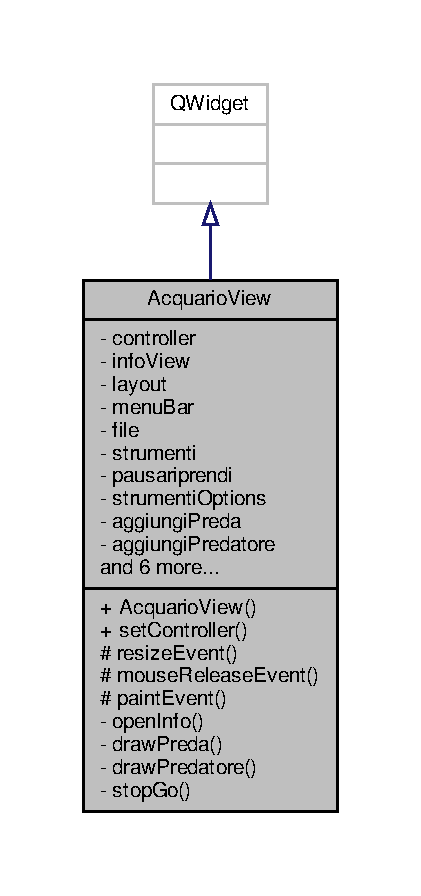
\includegraphics[width=202pt]{classAcquarioView__inherit__graph}
\end{center}
\end{figure}


Collaboration diagram for Acquario\+View\+:\nopagebreak
\begin{figure}[H]
\begin{center}
\leavevmode
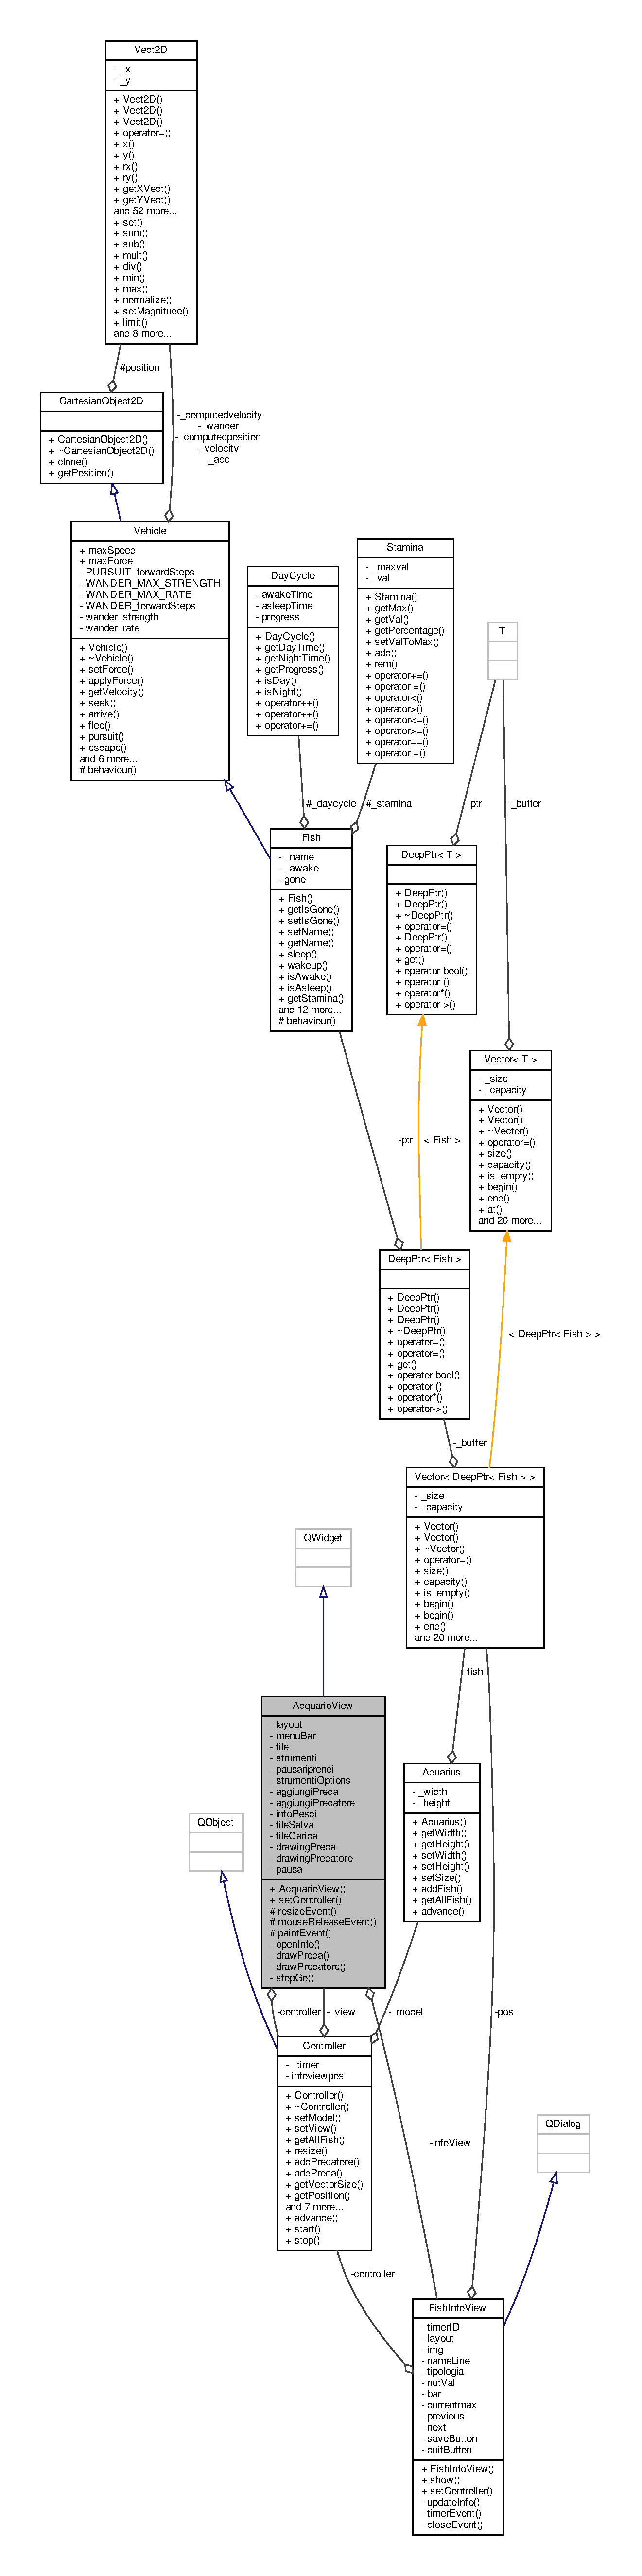
\includegraphics[height=550pt]{classAcquarioView__coll__graph}
\end{center}
\end{figure}
\subsection*{Public Member Functions}
\begin{DoxyCompactItemize}
\item 
\hyperlink{classAcquarioView_a5ac370a34350600cef09645040a3d6a0_a5ac370a34350600cef09645040a3d6a0}{Acquario\+View} (Q\+Widget $\ast$parent=nullptr)
\item 
void \hyperlink{classAcquarioView_a51cd9c97070c369e78cc8aa2c469f32f_a51cd9c97070c369e78cc8aa2c469f32f}{set\+Controller} (\hyperlink{classController}{Controller} $\ast$c)
\end{DoxyCompactItemize}
\subsection*{Protected Member Functions}
\begin{DoxyCompactItemize}
\item 
void \hyperlink{classAcquarioView_a0e079aa6c82990024c12b64933c3f1a9_a0e079aa6c82990024c12b64933c3f1a9}{resize\+Event} (Q\+Resize\+Event $\ast$) override
\item 
void \hyperlink{classAcquarioView_a147fcc39de40876b6fe694fff6f16616_a147fcc39de40876b6fe694fff6f16616}{mouse\+Release\+Event} (Q\+Mouse\+Event $\ast$) override
\item 
void \hyperlink{classAcquarioView_a1cc4e4cb7eee48bc6022523dc17f0c77_a1cc4e4cb7eee48bc6022523dc17f0c77}{paint\+Event} (Q\+Paint\+Event $\ast$) override
\end{DoxyCompactItemize}
\subsection*{Private Slots}
\begin{DoxyCompactItemize}
\item 
void \hyperlink{classAcquarioView_a30ae8edae52647aaf9b3386cf6991b72_a30ae8edae52647aaf9b3386cf6991b72}{open\+Info} ()
\item 
void \hyperlink{classAcquarioView_a39825ed2402d0cae4c9a7bbc050c21be_a39825ed2402d0cae4c9a7bbc050c21be}{draw\+Preda} ()
\item 
void \hyperlink{classAcquarioView_ac515fba6397d1fb32b92b6de5c08bc64_ac515fba6397d1fb32b92b6de5c08bc64}{draw\+Predatore} ()
\item 
void \hyperlink{classAcquarioView_a1387d7b13dd4969307de38b915b2b4d4_a1387d7b13dd4969307de38b915b2b4d4}{stop\+Go} ()
\end{DoxyCompactItemize}
\subsection*{Private Attributes}
\begin{DoxyCompactItemize}
\item 
\hyperlink{classController}{Controller} $\ast$ \hyperlink{classAcquarioView_a894c6c7ad89ce30db47c7c7ba37f6469_a894c6c7ad89ce30db47c7c7ba37f6469}{controller}
\item 
\hyperlink{classFishInfoView}{Fish\+Info\+View} $\ast$ \hyperlink{classAcquarioView_a7f0e96bf4bf69b1bb9c6bd6ef364145c_a7f0e96bf4bf69b1bb9c6bd6ef364145c}{info\+View}
\item 
Q\+V\+Box\+Layout $\ast$ \hyperlink{classAcquarioView_acbb6fc02e53b4b158643ee72fd1b1a43_acbb6fc02e53b4b158643ee72fd1b1a43}{layout}
\item 
Q\+Menu\+Bar $\ast$ \hyperlink{classAcquarioView_ac6a3b6a8febb40759c2bc3555995e46d_ac6a3b6a8febb40759c2bc3555995e46d}{menu\+Bar}
\item 
Q\+Menu $\ast$ \hyperlink{classAcquarioView_a794d97486873aa3cc187bed6aff3b1af_a794d97486873aa3cc187bed6aff3b1af}{file}
\item 
Q\+Menu $\ast$ \hyperlink{classAcquarioView_af3886eb0647eaaff7412fec6ba751d9c_af3886eb0647eaaff7412fec6ba751d9c}{strumenti}
\item 
Q\+Action $\ast$ \hyperlink{classAcquarioView_aa22b52c8af90c99a62fce96db94923dc_aa22b52c8af90c99a62fce96db94923dc}{pausariprendi}
\item 
Q\+Action\+Group $\ast$ \hyperlink{classAcquarioView_a254259de7a6667b127571170f362506f_a254259de7a6667b127571170f362506f}{strumenti\+Options}
\item 
Q\+Action $\ast$ \hyperlink{classAcquarioView_a0fc099b6a1ffefac21078ae1ff2c506c_a0fc099b6a1ffefac21078ae1ff2c506c}{aggiungi\+Preda}
\item 
Q\+Action $\ast$ \hyperlink{classAcquarioView_aaedc3e272850487836d7d3f2eca5f871_aaedc3e272850487836d7d3f2eca5f871}{aggiungi\+Predatore}
\item 
Q\+Action $\ast$ \hyperlink{classAcquarioView_a5e7f261dac213f74670d0e5345049045_a5e7f261dac213f74670d0e5345049045}{info\+Pesci}
\item 
Q\+Action $\ast$ \hyperlink{classAcquarioView_aa63343f4d1c27494bbe047211e315155_aa63343f4d1c27494bbe047211e315155}{file\+Salva}
\item 
Q\+Action $\ast$ \hyperlink{classAcquarioView_a91736ae2873ab1e8de4a792b832cef16_a91736ae2873ab1e8de4a792b832cef16}{file\+Carica}
\item 
bool \hyperlink{classAcquarioView_a24e948237068ccc38d460321e773664c_a24e948237068ccc38d460321e773664c}{drawing\+Preda}
\item 
bool \hyperlink{classAcquarioView_acf303ad47051a2c4ecc255c22b949807_acf303ad47051a2c4ecc255c22b949807}{drawing\+Predatore}
\item 
bool \hyperlink{classAcquarioView_a055ea31340de5ba6a555840010d7ffbc_a055ea31340de5ba6a555840010d7ffbc}{pausa}
\end{DoxyCompactItemize}


\subsection{Constructor \& Destructor Documentation}
\mbox{\Hypertarget{classAcquarioView_a5ac370a34350600cef09645040a3d6a0_a5ac370a34350600cef09645040a3d6a0}\label{classAcquarioView_a5ac370a34350600cef09645040a3d6a0_a5ac370a34350600cef09645040a3d6a0}} 
\index{Acquario\+View@{Acquario\+View}!Acquario\+View@{Acquario\+View}}
\index{Acquario\+View@{Acquario\+View}!Acquario\+View@{Acquario\+View}}
\subsubsection{\texorpdfstring{Acquario\+View()}{AcquarioView()}}
{\footnotesize\ttfamily Acquario\+View\+::\+Acquario\+View (\begin{DoxyParamCaption}\item[{Q\+Widget $\ast$}]{parent = {\ttfamily nullptr} }\end{DoxyParamCaption})\hspace{0.3cm}{\ttfamily [explicit]}}



\subsection{Member Function Documentation}
\mbox{\Hypertarget{classAcquarioView_a39825ed2402d0cae4c9a7bbc050c21be_a39825ed2402d0cae4c9a7bbc050c21be}\label{classAcquarioView_a39825ed2402d0cae4c9a7bbc050c21be_a39825ed2402d0cae4c9a7bbc050c21be}} 
\index{Acquario\+View@{Acquario\+View}!draw\+Preda@{draw\+Preda}}
\index{draw\+Preda@{draw\+Preda}!Acquario\+View@{Acquario\+View}}
\subsubsection{\texorpdfstring{draw\+Preda}{drawPreda}}
{\footnotesize\ttfamily void Acquario\+View\+::draw\+Preda (\begin{DoxyParamCaption}{ }\end{DoxyParamCaption})\hspace{0.3cm}{\ttfamily [private]}, {\ttfamily [slot]}}

\mbox{\Hypertarget{classAcquarioView_ac515fba6397d1fb32b92b6de5c08bc64_ac515fba6397d1fb32b92b6de5c08bc64}\label{classAcquarioView_ac515fba6397d1fb32b92b6de5c08bc64_ac515fba6397d1fb32b92b6de5c08bc64}} 
\index{Acquario\+View@{Acquario\+View}!draw\+Predatore@{draw\+Predatore}}
\index{draw\+Predatore@{draw\+Predatore}!Acquario\+View@{Acquario\+View}}
\subsubsection{\texorpdfstring{draw\+Predatore}{drawPredatore}}
{\footnotesize\ttfamily void Acquario\+View\+::draw\+Predatore (\begin{DoxyParamCaption}{ }\end{DoxyParamCaption})\hspace{0.3cm}{\ttfamily [private]}, {\ttfamily [slot]}}

\mbox{\Hypertarget{classAcquarioView_a147fcc39de40876b6fe694fff6f16616_a147fcc39de40876b6fe694fff6f16616}\label{classAcquarioView_a147fcc39de40876b6fe694fff6f16616_a147fcc39de40876b6fe694fff6f16616}} 
\index{Acquario\+View@{Acquario\+View}!mouse\+Release\+Event@{mouse\+Release\+Event}}
\index{mouse\+Release\+Event@{mouse\+Release\+Event}!Acquario\+View@{Acquario\+View}}
\subsubsection{\texorpdfstring{mouse\+Release\+Event()}{mouseReleaseEvent()}}
{\footnotesize\ttfamily void Acquario\+View\+::mouse\+Release\+Event (\begin{DoxyParamCaption}\item[{Q\+Mouse\+Event $\ast$}]{event }\end{DoxyParamCaption})\hspace{0.3cm}{\ttfamily [override]}, {\ttfamily [protected]}}

\mbox{\Hypertarget{classAcquarioView_a30ae8edae52647aaf9b3386cf6991b72_a30ae8edae52647aaf9b3386cf6991b72}\label{classAcquarioView_a30ae8edae52647aaf9b3386cf6991b72_a30ae8edae52647aaf9b3386cf6991b72}} 
\index{Acquario\+View@{Acquario\+View}!open\+Info@{open\+Info}}
\index{open\+Info@{open\+Info}!Acquario\+View@{Acquario\+View}}
\subsubsection{\texorpdfstring{open\+Info}{openInfo}}
{\footnotesize\ttfamily void Acquario\+View\+::open\+Info (\begin{DoxyParamCaption}{ }\end{DoxyParamCaption})\hspace{0.3cm}{\ttfamily [private]}, {\ttfamily [slot]}}

\mbox{\Hypertarget{classAcquarioView_a1cc4e4cb7eee48bc6022523dc17f0c77_a1cc4e4cb7eee48bc6022523dc17f0c77}\label{classAcquarioView_a1cc4e4cb7eee48bc6022523dc17f0c77_a1cc4e4cb7eee48bc6022523dc17f0c77}} 
\index{Acquario\+View@{Acquario\+View}!paint\+Event@{paint\+Event}}
\index{paint\+Event@{paint\+Event}!Acquario\+View@{Acquario\+View}}
\subsubsection{\texorpdfstring{paint\+Event()}{paintEvent()}}
{\footnotesize\ttfamily void Acquario\+View\+::paint\+Event (\begin{DoxyParamCaption}\item[{Q\+Paint\+Event $\ast$}]{ }\end{DoxyParamCaption})\hspace{0.3cm}{\ttfamily [override]}, {\ttfamily [protected]}}

\mbox{\Hypertarget{classAcquarioView_a0e079aa6c82990024c12b64933c3f1a9_a0e079aa6c82990024c12b64933c3f1a9}\label{classAcquarioView_a0e079aa6c82990024c12b64933c3f1a9_a0e079aa6c82990024c12b64933c3f1a9}} 
\index{Acquario\+View@{Acquario\+View}!resize\+Event@{resize\+Event}}
\index{resize\+Event@{resize\+Event}!Acquario\+View@{Acquario\+View}}
\subsubsection{\texorpdfstring{resize\+Event()}{resizeEvent()}}
{\footnotesize\ttfamily void Acquario\+View\+::resize\+Event (\begin{DoxyParamCaption}\item[{Q\+Resize\+Event $\ast$}]{event }\end{DoxyParamCaption})\hspace{0.3cm}{\ttfamily [override]}, {\ttfamily [protected]}}

\mbox{\Hypertarget{classAcquarioView_a51cd9c97070c369e78cc8aa2c469f32f_a51cd9c97070c369e78cc8aa2c469f32f}\label{classAcquarioView_a51cd9c97070c369e78cc8aa2c469f32f_a51cd9c97070c369e78cc8aa2c469f32f}} 
\index{Acquario\+View@{Acquario\+View}!set\+Controller@{set\+Controller}}
\index{set\+Controller@{set\+Controller}!Acquario\+View@{Acquario\+View}}
\subsubsection{\texorpdfstring{set\+Controller()}{setController()}}
{\footnotesize\ttfamily void Acquario\+View\+::set\+Controller (\begin{DoxyParamCaption}\item[{\hyperlink{classController}{Controller} $\ast$}]{c }\end{DoxyParamCaption})}

\mbox{\Hypertarget{classAcquarioView_a1387d7b13dd4969307de38b915b2b4d4_a1387d7b13dd4969307de38b915b2b4d4}\label{classAcquarioView_a1387d7b13dd4969307de38b915b2b4d4_a1387d7b13dd4969307de38b915b2b4d4}} 
\index{Acquario\+View@{Acquario\+View}!stop\+Go@{stop\+Go}}
\index{stop\+Go@{stop\+Go}!Acquario\+View@{Acquario\+View}}
\subsubsection{\texorpdfstring{stop\+Go}{stopGo}}
{\footnotesize\ttfamily void Acquario\+View\+::stop\+Go (\begin{DoxyParamCaption}{ }\end{DoxyParamCaption})\hspace{0.3cm}{\ttfamily [private]}, {\ttfamily [slot]}}



\subsection{Member Data Documentation}
\mbox{\Hypertarget{classAcquarioView_a0fc099b6a1ffefac21078ae1ff2c506c_a0fc099b6a1ffefac21078ae1ff2c506c}\label{classAcquarioView_a0fc099b6a1ffefac21078ae1ff2c506c_a0fc099b6a1ffefac21078ae1ff2c506c}} 
\index{Acquario\+View@{Acquario\+View}!aggiungi\+Preda@{aggiungi\+Preda}}
\index{aggiungi\+Preda@{aggiungi\+Preda}!Acquario\+View@{Acquario\+View}}
\subsubsection{\texorpdfstring{aggiungi\+Preda}{aggiungiPreda}}
{\footnotesize\ttfamily Q\+Action$\ast$ Acquario\+View\+::aggiungi\+Preda\hspace{0.3cm}{\ttfamily [private]}}

\mbox{\Hypertarget{classAcquarioView_aaedc3e272850487836d7d3f2eca5f871_aaedc3e272850487836d7d3f2eca5f871}\label{classAcquarioView_aaedc3e272850487836d7d3f2eca5f871_aaedc3e272850487836d7d3f2eca5f871}} 
\index{Acquario\+View@{Acquario\+View}!aggiungi\+Predatore@{aggiungi\+Predatore}}
\index{aggiungi\+Predatore@{aggiungi\+Predatore}!Acquario\+View@{Acquario\+View}}
\subsubsection{\texorpdfstring{aggiungi\+Predatore}{aggiungiPredatore}}
{\footnotesize\ttfamily Q\+Action$\ast$ Acquario\+View\+::aggiungi\+Predatore\hspace{0.3cm}{\ttfamily [private]}}

\mbox{\Hypertarget{classAcquarioView_a894c6c7ad89ce30db47c7c7ba37f6469_a894c6c7ad89ce30db47c7c7ba37f6469}\label{classAcquarioView_a894c6c7ad89ce30db47c7c7ba37f6469_a894c6c7ad89ce30db47c7c7ba37f6469}} 
\index{Acquario\+View@{Acquario\+View}!controller@{controller}}
\index{controller@{controller}!Acquario\+View@{Acquario\+View}}
\subsubsection{\texorpdfstring{controller}{controller}}
{\footnotesize\ttfamily \hyperlink{classController}{Controller}$\ast$ Acquario\+View\+::controller\hspace{0.3cm}{\ttfamily [private]}}

\mbox{\Hypertarget{classAcquarioView_a24e948237068ccc38d460321e773664c_a24e948237068ccc38d460321e773664c}\label{classAcquarioView_a24e948237068ccc38d460321e773664c_a24e948237068ccc38d460321e773664c}} 
\index{Acquario\+View@{Acquario\+View}!drawing\+Preda@{drawing\+Preda}}
\index{drawing\+Preda@{drawing\+Preda}!Acquario\+View@{Acquario\+View}}
\subsubsection{\texorpdfstring{drawing\+Preda}{drawingPreda}}
{\footnotesize\ttfamily bool Acquario\+View\+::drawing\+Preda\hspace{0.3cm}{\ttfamily [private]}}

\mbox{\Hypertarget{classAcquarioView_acf303ad47051a2c4ecc255c22b949807_acf303ad47051a2c4ecc255c22b949807}\label{classAcquarioView_acf303ad47051a2c4ecc255c22b949807_acf303ad47051a2c4ecc255c22b949807}} 
\index{Acquario\+View@{Acquario\+View}!drawing\+Predatore@{drawing\+Predatore}}
\index{drawing\+Predatore@{drawing\+Predatore}!Acquario\+View@{Acquario\+View}}
\subsubsection{\texorpdfstring{drawing\+Predatore}{drawingPredatore}}
{\footnotesize\ttfamily bool Acquario\+View\+::drawing\+Predatore\hspace{0.3cm}{\ttfamily [private]}}

\mbox{\Hypertarget{classAcquarioView_a794d97486873aa3cc187bed6aff3b1af_a794d97486873aa3cc187bed6aff3b1af}\label{classAcquarioView_a794d97486873aa3cc187bed6aff3b1af_a794d97486873aa3cc187bed6aff3b1af}} 
\index{Acquario\+View@{Acquario\+View}!file@{file}}
\index{file@{file}!Acquario\+View@{Acquario\+View}}
\subsubsection{\texorpdfstring{file}{file}}
{\footnotesize\ttfamily Q\+Menu$\ast$ Acquario\+View\+::file\hspace{0.3cm}{\ttfamily [private]}}

\mbox{\Hypertarget{classAcquarioView_a91736ae2873ab1e8de4a792b832cef16_a91736ae2873ab1e8de4a792b832cef16}\label{classAcquarioView_a91736ae2873ab1e8de4a792b832cef16_a91736ae2873ab1e8de4a792b832cef16}} 
\index{Acquario\+View@{Acquario\+View}!file\+Carica@{file\+Carica}}
\index{file\+Carica@{file\+Carica}!Acquario\+View@{Acquario\+View}}
\subsubsection{\texorpdfstring{file\+Carica}{fileCarica}}
{\footnotesize\ttfamily Q\+Action$\ast$ Acquario\+View\+::file\+Carica\hspace{0.3cm}{\ttfamily [private]}}

\mbox{\Hypertarget{classAcquarioView_aa63343f4d1c27494bbe047211e315155_aa63343f4d1c27494bbe047211e315155}\label{classAcquarioView_aa63343f4d1c27494bbe047211e315155_aa63343f4d1c27494bbe047211e315155}} 
\index{Acquario\+View@{Acquario\+View}!file\+Salva@{file\+Salva}}
\index{file\+Salva@{file\+Salva}!Acquario\+View@{Acquario\+View}}
\subsubsection{\texorpdfstring{file\+Salva}{fileSalva}}
{\footnotesize\ttfamily Q\+Action$\ast$ Acquario\+View\+::file\+Salva\hspace{0.3cm}{\ttfamily [private]}}

\mbox{\Hypertarget{classAcquarioView_a5e7f261dac213f74670d0e5345049045_a5e7f261dac213f74670d0e5345049045}\label{classAcquarioView_a5e7f261dac213f74670d0e5345049045_a5e7f261dac213f74670d0e5345049045}} 
\index{Acquario\+View@{Acquario\+View}!info\+Pesci@{info\+Pesci}}
\index{info\+Pesci@{info\+Pesci}!Acquario\+View@{Acquario\+View}}
\subsubsection{\texorpdfstring{info\+Pesci}{infoPesci}}
{\footnotesize\ttfamily Q\+Action$\ast$ Acquario\+View\+::info\+Pesci\hspace{0.3cm}{\ttfamily [private]}}

\mbox{\Hypertarget{classAcquarioView_a7f0e96bf4bf69b1bb9c6bd6ef364145c_a7f0e96bf4bf69b1bb9c6bd6ef364145c}\label{classAcquarioView_a7f0e96bf4bf69b1bb9c6bd6ef364145c_a7f0e96bf4bf69b1bb9c6bd6ef364145c}} 
\index{Acquario\+View@{Acquario\+View}!info\+View@{info\+View}}
\index{info\+View@{info\+View}!Acquario\+View@{Acquario\+View}}
\subsubsection{\texorpdfstring{info\+View}{infoView}}
{\footnotesize\ttfamily \hyperlink{classFishInfoView}{Fish\+Info\+View}$\ast$ Acquario\+View\+::info\+View\hspace{0.3cm}{\ttfamily [private]}}

\mbox{\Hypertarget{classAcquarioView_acbb6fc02e53b4b158643ee72fd1b1a43_acbb6fc02e53b4b158643ee72fd1b1a43}\label{classAcquarioView_acbb6fc02e53b4b158643ee72fd1b1a43_acbb6fc02e53b4b158643ee72fd1b1a43}} 
\index{Acquario\+View@{Acquario\+View}!layout@{layout}}
\index{layout@{layout}!Acquario\+View@{Acquario\+View}}
\subsubsection{\texorpdfstring{layout}{layout}}
{\footnotesize\ttfamily Q\+V\+Box\+Layout$\ast$ Acquario\+View\+::layout\hspace{0.3cm}{\ttfamily [private]}}

\mbox{\Hypertarget{classAcquarioView_ac6a3b6a8febb40759c2bc3555995e46d_ac6a3b6a8febb40759c2bc3555995e46d}\label{classAcquarioView_ac6a3b6a8febb40759c2bc3555995e46d_ac6a3b6a8febb40759c2bc3555995e46d}} 
\index{Acquario\+View@{Acquario\+View}!menu\+Bar@{menu\+Bar}}
\index{menu\+Bar@{menu\+Bar}!Acquario\+View@{Acquario\+View}}
\subsubsection{\texorpdfstring{menu\+Bar}{menuBar}}
{\footnotesize\ttfamily Q\+Menu\+Bar$\ast$ Acquario\+View\+::menu\+Bar\hspace{0.3cm}{\ttfamily [private]}}

\mbox{\Hypertarget{classAcquarioView_a055ea31340de5ba6a555840010d7ffbc_a055ea31340de5ba6a555840010d7ffbc}\label{classAcquarioView_a055ea31340de5ba6a555840010d7ffbc_a055ea31340de5ba6a555840010d7ffbc}} 
\index{Acquario\+View@{Acquario\+View}!pausa@{pausa}}
\index{pausa@{pausa}!Acquario\+View@{Acquario\+View}}
\subsubsection{\texorpdfstring{pausa}{pausa}}
{\footnotesize\ttfamily bool Acquario\+View\+::pausa\hspace{0.3cm}{\ttfamily [private]}}

\mbox{\Hypertarget{classAcquarioView_aa22b52c8af90c99a62fce96db94923dc_aa22b52c8af90c99a62fce96db94923dc}\label{classAcquarioView_aa22b52c8af90c99a62fce96db94923dc_aa22b52c8af90c99a62fce96db94923dc}} 
\index{Acquario\+View@{Acquario\+View}!pausariprendi@{pausariprendi}}
\index{pausariprendi@{pausariprendi}!Acquario\+View@{Acquario\+View}}
\subsubsection{\texorpdfstring{pausariprendi}{pausariprendi}}
{\footnotesize\ttfamily Q\+Action$\ast$ Acquario\+View\+::pausariprendi\hspace{0.3cm}{\ttfamily [private]}}

\mbox{\Hypertarget{classAcquarioView_af3886eb0647eaaff7412fec6ba751d9c_af3886eb0647eaaff7412fec6ba751d9c}\label{classAcquarioView_af3886eb0647eaaff7412fec6ba751d9c_af3886eb0647eaaff7412fec6ba751d9c}} 
\index{Acquario\+View@{Acquario\+View}!strumenti@{strumenti}}
\index{strumenti@{strumenti}!Acquario\+View@{Acquario\+View}}
\subsubsection{\texorpdfstring{strumenti}{strumenti}}
{\footnotesize\ttfamily Q\+Menu$\ast$ Acquario\+View\+::strumenti\hspace{0.3cm}{\ttfamily [private]}}

\mbox{\Hypertarget{classAcquarioView_a254259de7a6667b127571170f362506f_a254259de7a6667b127571170f362506f}\label{classAcquarioView_a254259de7a6667b127571170f362506f_a254259de7a6667b127571170f362506f}} 
\index{Acquario\+View@{Acquario\+View}!strumenti\+Options@{strumenti\+Options}}
\index{strumenti\+Options@{strumenti\+Options}!Acquario\+View@{Acquario\+View}}
\subsubsection{\texorpdfstring{strumenti\+Options}{strumentiOptions}}
{\footnotesize\ttfamily Q\+Action\+Group$\ast$ Acquario\+View\+::strumenti\+Options\hspace{0.3cm}{\ttfamily [private]}}



The documentation for this class was generated from the following files\+:\begin{DoxyCompactItemize}
\item 
include/\hyperlink{acquarioview_8hpp}{acquarioview.\+hpp}\item 
src/\hyperlink{acquarioview_8cpp}{acquarioview.\+cpp}\end{DoxyCompactItemize}

\hypertarget{classAquarius}{}\section{Aquarius Class Reference}
\label{classAquarius}\index{Aquarius@{Aquarius}}


{\ttfamily \#include $<$aquarius.\+hpp$>$}



Collaboration diagram for Aquarius\+:\nopagebreak
\begin{figure}[H]
\begin{center}
\leavevmode
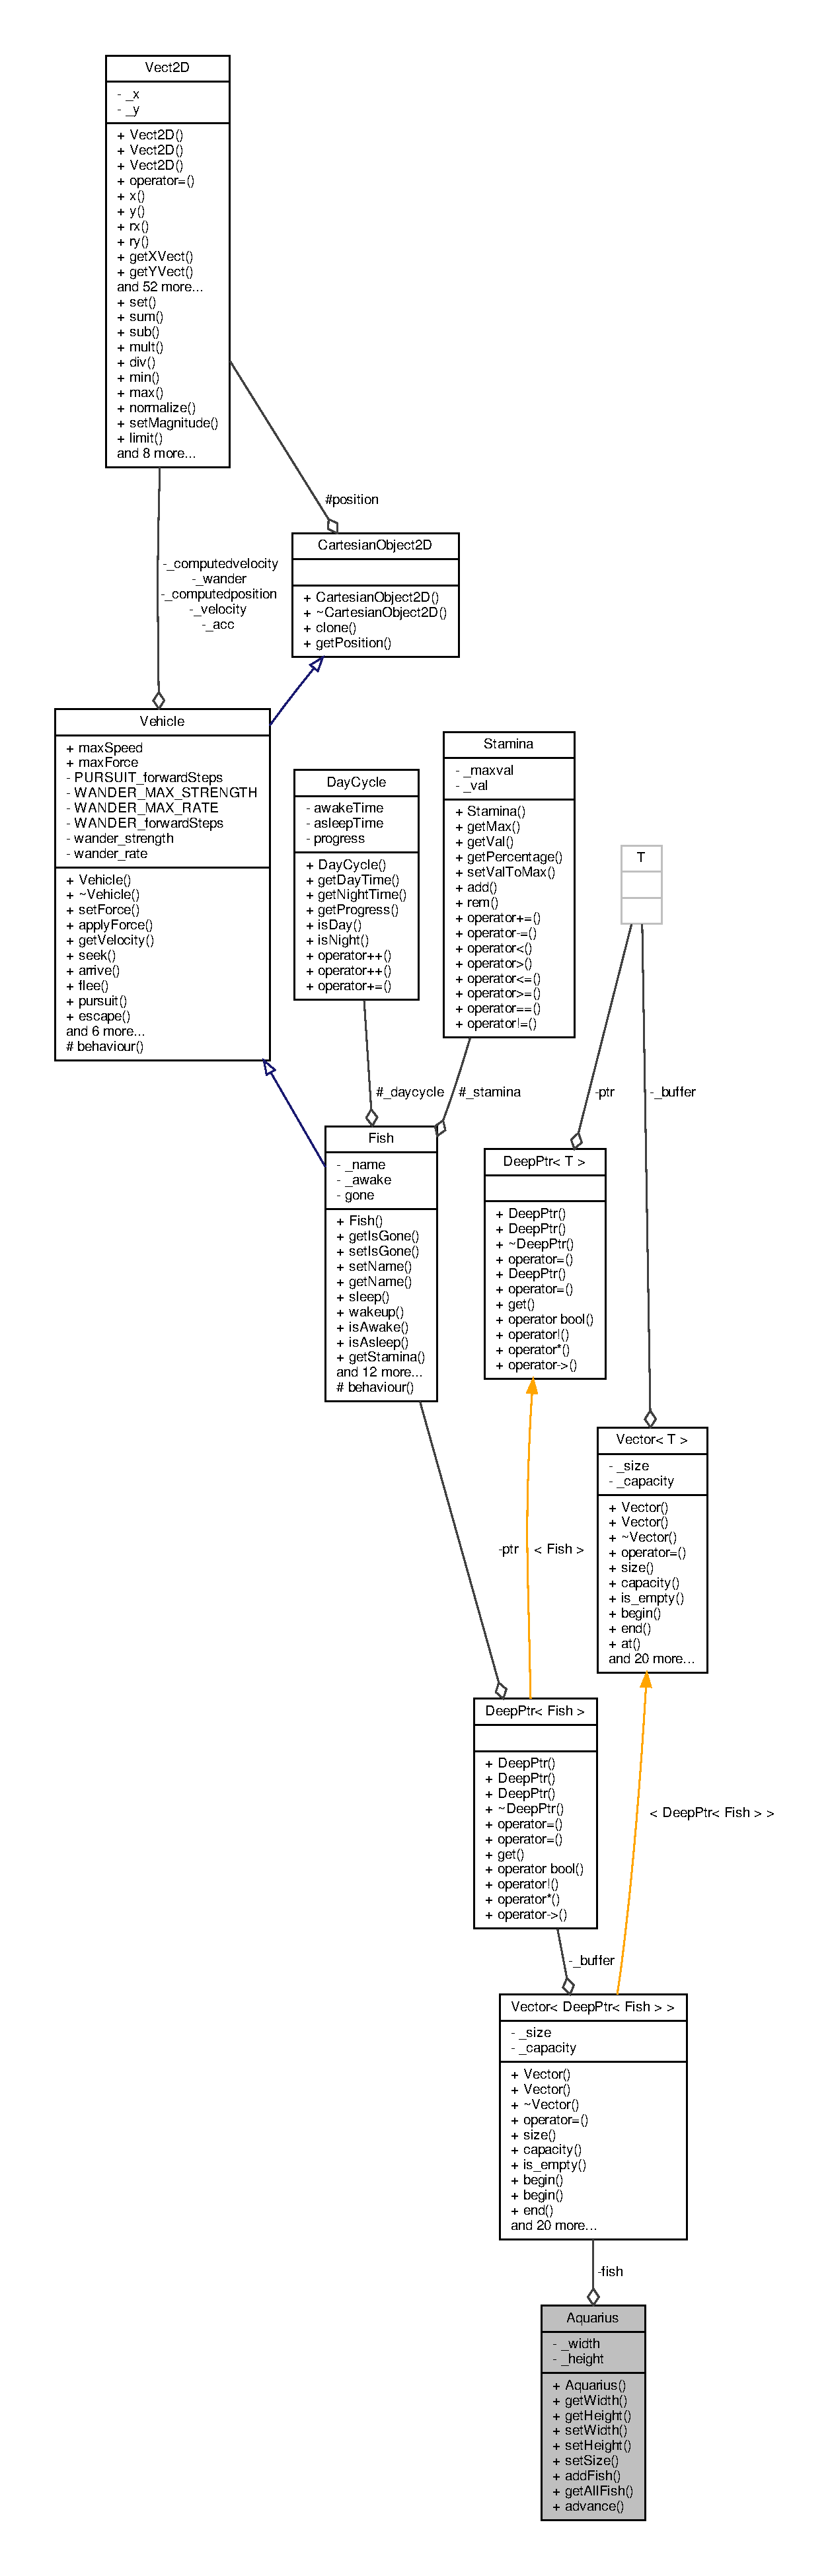
\includegraphics[height=550pt]{classAquarius__coll__graph}
\end{center}
\end{figure}
\subsection*{Public Member Functions}
\begin{DoxyCompactItemize}
\item 
\hyperlink{classAquarius_a7c8e40855d95468d8264ba0a1558d481_a7c8e40855d95468d8264ba0a1558d481}{Aquarius} (unsigned int=0, unsigned int=0)
\item 
unsigned int \hyperlink{classAquarius_a9cd1a0002fa16ca6f51ad4b00717c581_a9cd1a0002fa16ca6f51ad4b00717c581}{get\+Width} () const
\item 
unsigned int \hyperlink{classAquarius_a9f863c5458b9f5b21b6d0257b44ba433_a9f863c5458b9f5b21b6d0257b44ba433}{get\+Height} () const
\item 
void \hyperlink{classAquarius_a129d55d1a9e34354d1173f77f35f5ac8_a129d55d1a9e34354d1173f77f35f5ac8}{set\+Width} (unsigned int)
\item 
void \hyperlink{classAquarius_a64e999656f70edcfc6cedd4231638eb5_a64e999656f70edcfc6cedd4231638eb5}{set\+Height} (unsigned int)
\item 
void \hyperlink{classAquarius_ac357e8f719c2089527d2c493ca6aa1fc_ac357e8f719c2089527d2c493ca6aa1fc}{set\+Size} (unsigned int, unsigned int)
\item 
void \hyperlink{classAquarius_ab1d6d5d8f64be1cb8a0b9d0f0edea174_ab1d6d5d8f64be1cb8a0b9d0f0edea174}{add\+Fish} (\hyperlink{classFish}{Fish} $\ast$)
\item 
\hyperlink{classVector}{Vector}$<$ \hyperlink{classDeepPtr}{Deep\+Ptr}$<$ \hyperlink{classFish}{Fish} $>$ $>$ \& \hyperlink{classAquarius_a1bef6f16e9267d43d09d890783af1a09_a1bef6f16e9267d43d09d890783af1a09}{get\+All\+Fish} ()
\item 
void \hyperlink{classAquarius_a9fb56287ead8d2ac5b64098b95557bdd_a9fb56287ead8d2ac5b64098b95557bdd}{advance} ()
\end{DoxyCompactItemize}
\subsection*{Private Attributes}
\begin{DoxyCompactItemize}
\item 
unsigned int \hyperlink{classAquarius_a0ca48db776444e3513c0927127228dad_a0ca48db776444e3513c0927127228dad}{\+\_\+width}
\item 
unsigned int \hyperlink{classAquarius_a3b82543e9c69b03b53c76fbce4f945ea_a3b82543e9c69b03b53c76fbce4f945ea}{\+\_\+height}
\item 
\hyperlink{classVector}{Vector}$<$ \hyperlink{classDeepPtr}{Deep\+Ptr}$<$ \hyperlink{classFish}{Fish} $>$ $>$ \hyperlink{classAquarius_ad4c9e6cdbe69fbdc96cf8be68d1b9e82_ad4c9e6cdbe69fbdc96cf8be68d1b9e82}{fish}
\end{DoxyCompactItemize}


\subsection{Constructor \& Destructor Documentation}
\mbox{\Hypertarget{classAquarius_a7c8e40855d95468d8264ba0a1558d481_a7c8e40855d95468d8264ba0a1558d481}\label{classAquarius_a7c8e40855d95468d8264ba0a1558d481_a7c8e40855d95468d8264ba0a1558d481}} 
\index{Aquarius@{Aquarius}!Aquarius@{Aquarius}}
\index{Aquarius@{Aquarius}!Aquarius@{Aquarius}}
\subsubsection{\texorpdfstring{Aquarius()}{Aquarius()}}
{\footnotesize\ttfamily Aquarius\+::\+Aquarius (\begin{DoxyParamCaption}\item[{unsigned int}]{width = {\ttfamily 0},  }\item[{unsigned int}]{height = {\ttfamily 0} }\end{DoxyParamCaption})}



\subsection{Member Function Documentation}
\mbox{\Hypertarget{classAquarius_ab1d6d5d8f64be1cb8a0b9d0f0edea174_ab1d6d5d8f64be1cb8a0b9d0f0edea174}\label{classAquarius_ab1d6d5d8f64be1cb8a0b9d0f0edea174_ab1d6d5d8f64be1cb8a0b9d0f0edea174}} 
\index{Aquarius@{Aquarius}!add\+Fish@{add\+Fish}}
\index{add\+Fish@{add\+Fish}!Aquarius@{Aquarius}}
\subsubsection{\texorpdfstring{add\+Fish()}{addFish()}}
{\footnotesize\ttfamily void Aquarius\+::add\+Fish (\begin{DoxyParamCaption}\item[{\hyperlink{classFish}{Fish} $\ast$}]{v }\end{DoxyParamCaption})}

\mbox{\Hypertarget{classAquarius_a9fb56287ead8d2ac5b64098b95557bdd_a9fb56287ead8d2ac5b64098b95557bdd}\label{classAquarius_a9fb56287ead8d2ac5b64098b95557bdd_a9fb56287ead8d2ac5b64098b95557bdd}} 
\index{Aquarius@{Aquarius}!advance@{advance}}
\index{advance@{advance}!Aquarius@{Aquarius}}
\subsubsection{\texorpdfstring{advance()}{advance()}}
{\footnotesize\ttfamily void Aquarius\+::advance (\begin{DoxyParamCaption}{ }\end{DoxyParamCaption})}

\mbox{\Hypertarget{classAquarius_a1bef6f16e9267d43d09d890783af1a09_a1bef6f16e9267d43d09d890783af1a09}\label{classAquarius_a1bef6f16e9267d43d09d890783af1a09_a1bef6f16e9267d43d09d890783af1a09}} 
\index{Aquarius@{Aquarius}!get\+All\+Fish@{get\+All\+Fish}}
\index{get\+All\+Fish@{get\+All\+Fish}!Aquarius@{Aquarius}}
\subsubsection{\texorpdfstring{get\+All\+Fish()}{getAllFish()}}
{\footnotesize\ttfamily \hyperlink{classVector}{Vector}$<$ \hyperlink{classDeepPtr}{Deep\+Ptr}$<$ \hyperlink{classFish}{Fish} $>$ $>$ \& Aquarius\+::get\+All\+Fish (\begin{DoxyParamCaption}{ }\end{DoxyParamCaption})}

\mbox{\Hypertarget{classAquarius_a9f863c5458b9f5b21b6d0257b44ba433_a9f863c5458b9f5b21b6d0257b44ba433}\label{classAquarius_a9f863c5458b9f5b21b6d0257b44ba433_a9f863c5458b9f5b21b6d0257b44ba433}} 
\index{Aquarius@{Aquarius}!get\+Height@{get\+Height}}
\index{get\+Height@{get\+Height}!Aquarius@{Aquarius}}
\subsubsection{\texorpdfstring{get\+Height()}{getHeight()}}
{\footnotesize\ttfamily unsigned int Aquarius\+::get\+Height (\begin{DoxyParamCaption}{ }\end{DoxyParamCaption}) const}

\mbox{\Hypertarget{classAquarius_a9cd1a0002fa16ca6f51ad4b00717c581_a9cd1a0002fa16ca6f51ad4b00717c581}\label{classAquarius_a9cd1a0002fa16ca6f51ad4b00717c581_a9cd1a0002fa16ca6f51ad4b00717c581}} 
\index{Aquarius@{Aquarius}!get\+Width@{get\+Width}}
\index{get\+Width@{get\+Width}!Aquarius@{Aquarius}}
\subsubsection{\texorpdfstring{get\+Width()}{getWidth()}}
{\footnotesize\ttfamily unsigned int Aquarius\+::get\+Width (\begin{DoxyParamCaption}{ }\end{DoxyParamCaption}) const}

\mbox{\Hypertarget{classAquarius_a64e999656f70edcfc6cedd4231638eb5_a64e999656f70edcfc6cedd4231638eb5}\label{classAquarius_a64e999656f70edcfc6cedd4231638eb5_a64e999656f70edcfc6cedd4231638eb5}} 
\index{Aquarius@{Aquarius}!set\+Height@{set\+Height}}
\index{set\+Height@{set\+Height}!Aquarius@{Aquarius}}
\subsubsection{\texorpdfstring{set\+Height()}{setHeight()}}
{\footnotesize\ttfamily void Aquarius\+::set\+Height (\begin{DoxyParamCaption}\item[{unsigned int}]{height }\end{DoxyParamCaption})}

\mbox{\Hypertarget{classAquarius_ac357e8f719c2089527d2c493ca6aa1fc_ac357e8f719c2089527d2c493ca6aa1fc}\label{classAquarius_ac357e8f719c2089527d2c493ca6aa1fc_ac357e8f719c2089527d2c493ca6aa1fc}} 
\index{Aquarius@{Aquarius}!set\+Size@{set\+Size}}
\index{set\+Size@{set\+Size}!Aquarius@{Aquarius}}
\subsubsection{\texorpdfstring{set\+Size()}{setSize()}}
{\footnotesize\ttfamily void Aquarius\+::set\+Size (\begin{DoxyParamCaption}\item[{unsigned int}]{width,  }\item[{unsigned int}]{height }\end{DoxyParamCaption})}

\mbox{\Hypertarget{classAquarius_a129d55d1a9e34354d1173f77f35f5ac8_a129d55d1a9e34354d1173f77f35f5ac8}\label{classAquarius_a129d55d1a9e34354d1173f77f35f5ac8_a129d55d1a9e34354d1173f77f35f5ac8}} 
\index{Aquarius@{Aquarius}!set\+Width@{set\+Width}}
\index{set\+Width@{set\+Width}!Aquarius@{Aquarius}}
\subsubsection{\texorpdfstring{set\+Width()}{setWidth()}}
{\footnotesize\ttfamily void Aquarius\+::set\+Width (\begin{DoxyParamCaption}\item[{unsigned int}]{width }\end{DoxyParamCaption})}



\subsection{Member Data Documentation}
\mbox{\Hypertarget{classAquarius_a3b82543e9c69b03b53c76fbce4f945ea_a3b82543e9c69b03b53c76fbce4f945ea}\label{classAquarius_a3b82543e9c69b03b53c76fbce4f945ea_a3b82543e9c69b03b53c76fbce4f945ea}} 
\index{Aquarius@{Aquarius}!\+\_\+height@{\+\_\+height}}
\index{\+\_\+height@{\+\_\+height}!Aquarius@{Aquarius}}
\subsubsection{\texorpdfstring{\+\_\+height}{\_height}}
{\footnotesize\ttfamily unsigned int Aquarius\+::\+\_\+height\hspace{0.3cm}{\ttfamily [private]}}

\mbox{\Hypertarget{classAquarius_a0ca48db776444e3513c0927127228dad_a0ca48db776444e3513c0927127228dad}\label{classAquarius_a0ca48db776444e3513c0927127228dad_a0ca48db776444e3513c0927127228dad}} 
\index{Aquarius@{Aquarius}!\+\_\+width@{\+\_\+width}}
\index{\+\_\+width@{\+\_\+width}!Aquarius@{Aquarius}}
\subsubsection{\texorpdfstring{\+\_\+width}{\_width}}
{\footnotesize\ttfamily unsigned int Aquarius\+::\+\_\+width\hspace{0.3cm}{\ttfamily [private]}}

\mbox{\Hypertarget{classAquarius_ad4c9e6cdbe69fbdc96cf8be68d1b9e82_ad4c9e6cdbe69fbdc96cf8be68d1b9e82}\label{classAquarius_ad4c9e6cdbe69fbdc96cf8be68d1b9e82_ad4c9e6cdbe69fbdc96cf8be68d1b9e82}} 
\index{Aquarius@{Aquarius}!fish@{fish}}
\index{fish@{fish}!Aquarius@{Aquarius}}
\subsubsection{\texorpdfstring{fish}{fish}}
{\footnotesize\ttfamily \hyperlink{classVector}{Vector}$<$\hyperlink{classDeepPtr}{Deep\+Ptr}$<$\hyperlink{classFish}{Fish}$>$ $>$ Aquarius\+::fish\hspace{0.3cm}{\ttfamily [private]}}



The documentation for this class was generated from the following files\+:\begin{DoxyCompactItemize}
\item 
include/\hyperlink{aquarius_8hpp}{aquarius.\+hpp}\item 
src/\hyperlink{aquarius_8cpp}{aquarius.\+cpp}\end{DoxyCompactItemize}

\hypertarget{classBSPTree}{}\section{B\+S\+P\+Tree$<$ T $>$ Class Template Reference}
\label{classBSPTree}\index{B\+S\+P\+Tree$<$ T $>$@{B\+S\+P\+Tree$<$ T $>$}}


{\ttfamily \#include $<$bsptree.\+hpp$>$}



Collaboration diagram for B\+S\+P\+Tree$<$ T $>$\+:\nopagebreak
\begin{figure}[H]
\begin{center}
\leavevmode
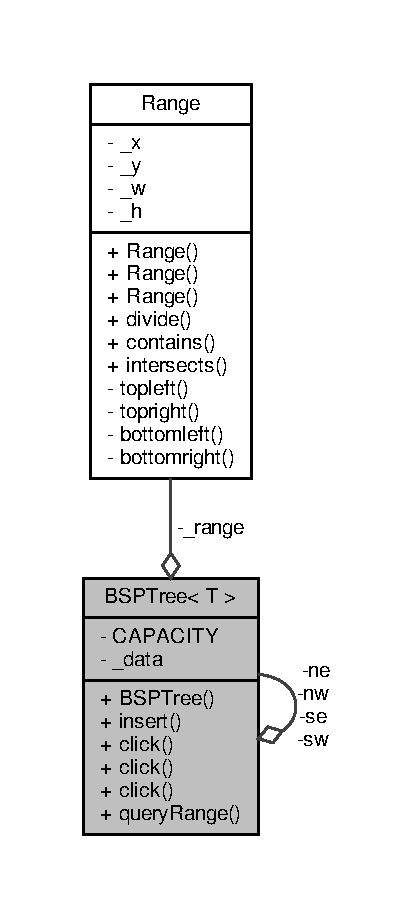
\includegraphics[width=199pt]{classBSPTree__coll__graph}
\end{center}
\end{figure}
\subsection*{Public Member Functions}
\begin{DoxyCompactItemize}
\item 
\hyperlink{classBSPTree_ac0d5688da625398b735b724afa22891c_ac0d5688da625398b735b724afa22891c}{B\+S\+P\+Tree} (const \hyperlink{classRange}{Range} \&range)
\item 
bool \hyperlink{classBSPTree_ac4d6edf03e621e59e96b27b4943d304c_ac4d6edf03e621e59e96b27b4943d304c}{insert} (const \hyperlink{classVect2D}{Vect2D} \&position, T $\ast$data)
\item 
T $\ast$ \hyperlink{classBSPTree_a3f713d6aeb66e8b1c1f35f06d49edcf1_a3f713d6aeb66e8b1c1f35f06d49edcf1}{click} (double x, double y, double halfsize)
\item 
T $\ast$ \hyperlink{classBSPTree_a442f2b98cf404a7467daea83fda59d9e_a442f2b98cf404a7467daea83fda59d9e}{click} (const \hyperlink{classVect2D}{Vect2D} \&position, double halfsize)
\item 
T $\ast$ \hyperlink{classBSPTree_a5dca4c571d2ad30c13b90710ad479df3_a5dca4c571d2ad30c13b90710ad479df3}{click} (const \hyperlink{classRange}{Range} \&r)
\item 
void \hyperlink{classBSPTree_a05d3d440bd02e164f450ef26fd94a2d9_a05d3d440bd02e164f450ef26fd94a2d9}{query\+Range} (const \hyperlink{classRange}{Range} \&r, std\+::vector$<$ T $\ast$$>$ \&v)
\end{DoxyCompactItemize}
\subsection*{Private Attributes}
\begin{DoxyCompactItemize}
\item 
\hyperlink{classRange}{Range} \hyperlink{classBSPTree_a9af2e4216eb728b7135b197b0e1c4dea_a9af2e4216eb728b7135b197b0e1c4dea}{\+\_\+range}
\item 
const unsigned int \hyperlink{classBSPTree_ac25b3f64ce4f4e49398978cab2382109_ac25b3f64ce4f4e49398978cab2382109}{C\+A\+P\+A\+C\+I\+TY} = 10
\item 
std\+::vector$<$ std\+::pair$<$ \hyperlink{classVect2D}{Vect2D}, T $\ast$ $>$ $>$ \hyperlink{classBSPTree_af60e625922e4eeb8647f5cd07d28dddd_af60e625922e4eeb8647f5cd07d28dddd}{\+\_\+data}
\item 
\hyperlink{classBSPTree}{B\+S\+P\+Tree} $\ast$ \hyperlink{classBSPTree_a1569e87d368a255fd0f9ba00ebae7949_a1569e87d368a255fd0f9ba00ebae7949}{nw}
\item 
\hyperlink{classBSPTree}{B\+S\+P\+Tree} $\ast$ \hyperlink{classBSPTree_aff1f52f86167389c6f35c03dcdda96b5_aff1f52f86167389c6f35c03dcdda96b5}{ne}
\item 
\hyperlink{classBSPTree}{B\+S\+P\+Tree} $\ast$ \hyperlink{classBSPTree_ae93464ee431a9bfdc211bb622b69342e_ae93464ee431a9bfdc211bb622b69342e}{sw}
\item 
\hyperlink{classBSPTree}{B\+S\+P\+Tree} $\ast$ \hyperlink{classBSPTree_a7f3b004aa986f92ab37af1069a7f1d0b_a7f3b004aa986f92ab37af1069a7f1d0b}{se}
\end{DoxyCompactItemize}


\subsection{Constructor \& Destructor Documentation}
\mbox{\Hypertarget{classBSPTree_ac0d5688da625398b735b724afa22891c_ac0d5688da625398b735b724afa22891c}\label{classBSPTree_ac0d5688da625398b735b724afa22891c_ac0d5688da625398b735b724afa22891c}} 
\index{B\+S\+P\+Tree@{B\+S\+P\+Tree}!B\+S\+P\+Tree@{B\+S\+P\+Tree}}
\index{B\+S\+P\+Tree@{B\+S\+P\+Tree}!B\+S\+P\+Tree@{B\+S\+P\+Tree}}
\subsubsection{\texorpdfstring{B\+S\+P\+Tree()}{BSPTree()}}
{\footnotesize\ttfamily template$<$class T $>$ \\
\hyperlink{classBSPTree}{B\+S\+P\+Tree}$<$ T $>$\+::\hyperlink{classBSPTree}{B\+S\+P\+Tree} (\begin{DoxyParamCaption}\item[{const \hyperlink{classRange}{Range} \&}]{range }\end{DoxyParamCaption})\hspace{0.3cm}{\ttfamily [inline]}}



\subsection{Member Function Documentation}
\mbox{\Hypertarget{classBSPTree_a3f713d6aeb66e8b1c1f35f06d49edcf1_a3f713d6aeb66e8b1c1f35f06d49edcf1}\label{classBSPTree_a3f713d6aeb66e8b1c1f35f06d49edcf1_a3f713d6aeb66e8b1c1f35f06d49edcf1}} 
\index{B\+S\+P\+Tree@{B\+S\+P\+Tree}!click@{click}}
\index{click@{click}!B\+S\+P\+Tree@{B\+S\+P\+Tree}}
\subsubsection{\texorpdfstring{click()}{click()}\hspace{0.1cm}{\footnotesize\ttfamily [1/3]}}
{\footnotesize\ttfamily template$<$class T $>$ \\
T$\ast$ \hyperlink{classBSPTree}{B\+S\+P\+Tree}$<$ T $>$\+::click (\begin{DoxyParamCaption}\item[{double}]{x,  }\item[{double}]{y,  }\item[{double}]{halfsize }\end{DoxyParamCaption})\hspace{0.3cm}{\ttfamily [inline]}}

\mbox{\Hypertarget{classBSPTree_a442f2b98cf404a7467daea83fda59d9e_a442f2b98cf404a7467daea83fda59d9e}\label{classBSPTree_a442f2b98cf404a7467daea83fda59d9e_a442f2b98cf404a7467daea83fda59d9e}} 
\index{B\+S\+P\+Tree@{B\+S\+P\+Tree}!click@{click}}
\index{click@{click}!B\+S\+P\+Tree@{B\+S\+P\+Tree}}
\subsubsection{\texorpdfstring{click()}{click()}\hspace{0.1cm}{\footnotesize\ttfamily [2/3]}}
{\footnotesize\ttfamily template$<$class T $>$ \\
T$\ast$ \hyperlink{classBSPTree}{B\+S\+P\+Tree}$<$ T $>$\+::click (\begin{DoxyParamCaption}\item[{const \hyperlink{classVect2D}{Vect2D} \&}]{position,  }\item[{double}]{halfsize }\end{DoxyParamCaption})\hspace{0.3cm}{\ttfamily [inline]}}

\mbox{\Hypertarget{classBSPTree_a5dca4c571d2ad30c13b90710ad479df3_a5dca4c571d2ad30c13b90710ad479df3}\label{classBSPTree_a5dca4c571d2ad30c13b90710ad479df3_a5dca4c571d2ad30c13b90710ad479df3}} 
\index{B\+S\+P\+Tree@{B\+S\+P\+Tree}!click@{click}}
\index{click@{click}!B\+S\+P\+Tree@{B\+S\+P\+Tree}}
\subsubsection{\texorpdfstring{click()}{click()}\hspace{0.1cm}{\footnotesize\ttfamily [3/3]}}
{\footnotesize\ttfamily template$<$class T $>$ \\
T$\ast$ \hyperlink{classBSPTree}{B\+S\+P\+Tree}$<$ T $>$\+::click (\begin{DoxyParamCaption}\item[{const \hyperlink{classRange}{Range} \&}]{r }\end{DoxyParamCaption})\hspace{0.3cm}{\ttfamily [inline]}}

\mbox{\Hypertarget{classBSPTree_ac4d6edf03e621e59e96b27b4943d304c_ac4d6edf03e621e59e96b27b4943d304c}\label{classBSPTree_ac4d6edf03e621e59e96b27b4943d304c_ac4d6edf03e621e59e96b27b4943d304c}} 
\index{B\+S\+P\+Tree@{B\+S\+P\+Tree}!insert@{insert}}
\index{insert@{insert}!B\+S\+P\+Tree@{B\+S\+P\+Tree}}
\subsubsection{\texorpdfstring{insert()}{insert()}}
{\footnotesize\ttfamily template$<$class T $>$ \\
bool \hyperlink{classBSPTree}{B\+S\+P\+Tree}$<$ T $>$\+::insert (\begin{DoxyParamCaption}\item[{const \hyperlink{classVect2D}{Vect2D} \&}]{position,  }\item[{T $\ast$}]{data }\end{DoxyParamCaption})\hspace{0.3cm}{\ttfamily [inline]}}

\mbox{\Hypertarget{classBSPTree_a05d3d440bd02e164f450ef26fd94a2d9_a05d3d440bd02e164f450ef26fd94a2d9}\label{classBSPTree_a05d3d440bd02e164f450ef26fd94a2d9_a05d3d440bd02e164f450ef26fd94a2d9}} 
\index{B\+S\+P\+Tree@{B\+S\+P\+Tree}!query\+Range@{query\+Range}}
\index{query\+Range@{query\+Range}!B\+S\+P\+Tree@{B\+S\+P\+Tree}}
\subsubsection{\texorpdfstring{query\+Range()}{queryRange()}}
{\footnotesize\ttfamily template$<$class T $>$ \\
void \hyperlink{classBSPTree}{B\+S\+P\+Tree}$<$ T $>$\+::query\+Range (\begin{DoxyParamCaption}\item[{const \hyperlink{classRange}{Range} \&}]{r,  }\item[{std\+::vector$<$ T $\ast$$>$ \&}]{v }\end{DoxyParamCaption})\hspace{0.3cm}{\ttfamily [inline]}}



\subsection{Member Data Documentation}
\mbox{\Hypertarget{classBSPTree_af60e625922e4eeb8647f5cd07d28dddd_af60e625922e4eeb8647f5cd07d28dddd}\label{classBSPTree_af60e625922e4eeb8647f5cd07d28dddd_af60e625922e4eeb8647f5cd07d28dddd}} 
\index{B\+S\+P\+Tree@{B\+S\+P\+Tree}!\+\_\+data@{\+\_\+data}}
\index{\+\_\+data@{\+\_\+data}!B\+S\+P\+Tree@{B\+S\+P\+Tree}}
\subsubsection{\texorpdfstring{\+\_\+data}{\_data}}
{\footnotesize\ttfamily template$<$class T $>$ \\
std\+::vector$<$std\+::pair$<$\hyperlink{classVect2D}{Vect2D}, T$\ast$$>$ $>$ \hyperlink{classBSPTree}{B\+S\+P\+Tree}$<$ T $>$\+::\+\_\+data\hspace{0.3cm}{\ttfamily [private]}}

\mbox{\Hypertarget{classBSPTree_a9af2e4216eb728b7135b197b0e1c4dea_a9af2e4216eb728b7135b197b0e1c4dea}\label{classBSPTree_a9af2e4216eb728b7135b197b0e1c4dea_a9af2e4216eb728b7135b197b0e1c4dea}} 
\index{B\+S\+P\+Tree@{B\+S\+P\+Tree}!\+\_\+range@{\+\_\+range}}
\index{\+\_\+range@{\+\_\+range}!B\+S\+P\+Tree@{B\+S\+P\+Tree}}
\subsubsection{\texorpdfstring{\+\_\+range}{\_range}}
{\footnotesize\ttfamily template$<$class T $>$ \\
\hyperlink{classRange}{Range} \hyperlink{classBSPTree}{B\+S\+P\+Tree}$<$ T $>$\+::\+\_\+range\hspace{0.3cm}{\ttfamily [private]}}

\mbox{\Hypertarget{classBSPTree_ac25b3f64ce4f4e49398978cab2382109_ac25b3f64ce4f4e49398978cab2382109}\label{classBSPTree_ac25b3f64ce4f4e49398978cab2382109_ac25b3f64ce4f4e49398978cab2382109}} 
\index{B\+S\+P\+Tree@{B\+S\+P\+Tree}!C\+A\+P\+A\+C\+I\+TY@{C\+A\+P\+A\+C\+I\+TY}}
\index{C\+A\+P\+A\+C\+I\+TY@{C\+A\+P\+A\+C\+I\+TY}!B\+S\+P\+Tree@{B\+S\+P\+Tree}}
\subsubsection{\texorpdfstring{C\+A\+P\+A\+C\+I\+TY}{CAPACITY}}
{\footnotesize\ttfamily template$<$class T $>$ \\
const unsigned int \hyperlink{classBSPTree}{B\+S\+P\+Tree}$<$ T $>$\+::C\+A\+P\+A\+C\+I\+TY = 10\hspace{0.3cm}{\ttfamily [private]}}

\mbox{\Hypertarget{classBSPTree_aff1f52f86167389c6f35c03dcdda96b5_aff1f52f86167389c6f35c03dcdda96b5}\label{classBSPTree_aff1f52f86167389c6f35c03dcdda96b5_aff1f52f86167389c6f35c03dcdda96b5}} 
\index{B\+S\+P\+Tree@{B\+S\+P\+Tree}!ne@{ne}}
\index{ne@{ne}!B\+S\+P\+Tree@{B\+S\+P\+Tree}}
\subsubsection{\texorpdfstring{ne}{ne}}
{\footnotesize\ttfamily template$<$class T $>$ \\
\hyperlink{classBSPTree}{B\+S\+P\+Tree}$\ast$ \hyperlink{classBSPTree}{B\+S\+P\+Tree}$<$ T $>$\+::ne\hspace{0.3cm}{\ttfamily [private]}}

\mbox{\Hypertarget{classBSPTree_a1569e87d368a255fd0f9ba00ebae7949_a1569e87d368a255fd0f9ba00ebae7949}\label{classBSPTree_a1569e87d368a255fd0f9ba00ebae7949_a1569e87d368a255fd0f9ba00ebae7949}} 
\index{B\+S\+P\+Tree@{B\+S\+P\+Tree}!nw@{nw}}
\index{nw@{nw}!B\+S\+P\+Tree@{B\+S\+P\+Tree}}
\subsubsection{\texorpdfstring{nw}{nw}}
{\footnotesize\ttfamily template$<$class T $>$ \\
\hyperlink{classBSPTree}{B\+S\+P\+Tree}$\ast$ \hyperlink{classBSPTree}{B\+S\+P\+Tree}$<$ T $>$\+::nw\hspace{0.3cm}{\ttfamily [private]}}

\mbox{\Hypertarget{classBSPTree_a7f3b004aa986f92ab37af1069a7f1d0b_a7f3b004aa986f92ab37af1069a7f1d0b}\label{classBSPTree_a7f3b004aa986f92ab37af1069a7f1d0b_a7f3b004aa986f92ab37af1069a7f1d0b}} 
\index{B\+S\+P\+Tree@{B\+S\+P\+Tree}!se@{se}}
\index{se@{se}!B\+S\+P\+Tree@{B\+S\+P\+Tree}}
\subsubsection{\texorpdfstring{se}{se}}
{\footnotesize\ttfamily template$<$class T $>$ \\
\hyperlink{classBSPTree}{B\+S\+P\+Tree}$\ast$ \hyperlink{classBSPTree}{B\+S\+P\+Tree}$<$ T $>$\+::se\hspace{0.3cm}{\ttfamily [private]}}

\mbox{\Hypertarget{classBSPTree_ae93464ee431a9bfdc211bb622b69342e_ae93464ee431a9bfdc211bb622b69342e}\label{classBSPTree_ae93464ee431a9bfdc211bb622b69342e_ae93464ee431a9bfdc211bb622b69342e}} 
\index{B\+S\+P\+Tree@{B\+S\+P\+Tree}!sw@{sw}}
\index{sw@{sw}!B\+S\+P\+Tree@{B\+S\+P\+Tree}}
\subsubsection{\texorpdfstring{sw}{sw}}
{\footnotesize\ttfamily template$<$class T $>$ \\
\hyperlink{classBSPTree}{B\+S\+P\+Tree}$\ast$ \hyperlink{classBSPTree}{B\+S\+P\+Tree}$<$ T $>$\+::sw\hspace{0.3cm}{\ttfamily [private]}}



The documentation for this class was generated from the following file\+:\begin{DoxyCompactItemize}
\item 
include/\hyperlink{bsptree_8hpp}{bsptree.\+hpp}\end{DoxyCompactItemize}

\hypertarget{classCartesianObject2D}{}\section{Cartesian\+Object2D Class Reference}
\label{classCartesianObject2D}\index{Cartesian\+Object2D@{Cartesian\+Object2D}}


{\ttfamily \#include $<$cartesianobject2d.\+hpp$>$}



Inheritance diagram for Cartesian\+Object2D\+:\nopagebreak
\begin{figure}[H]
\begin{center}
\leavevmode
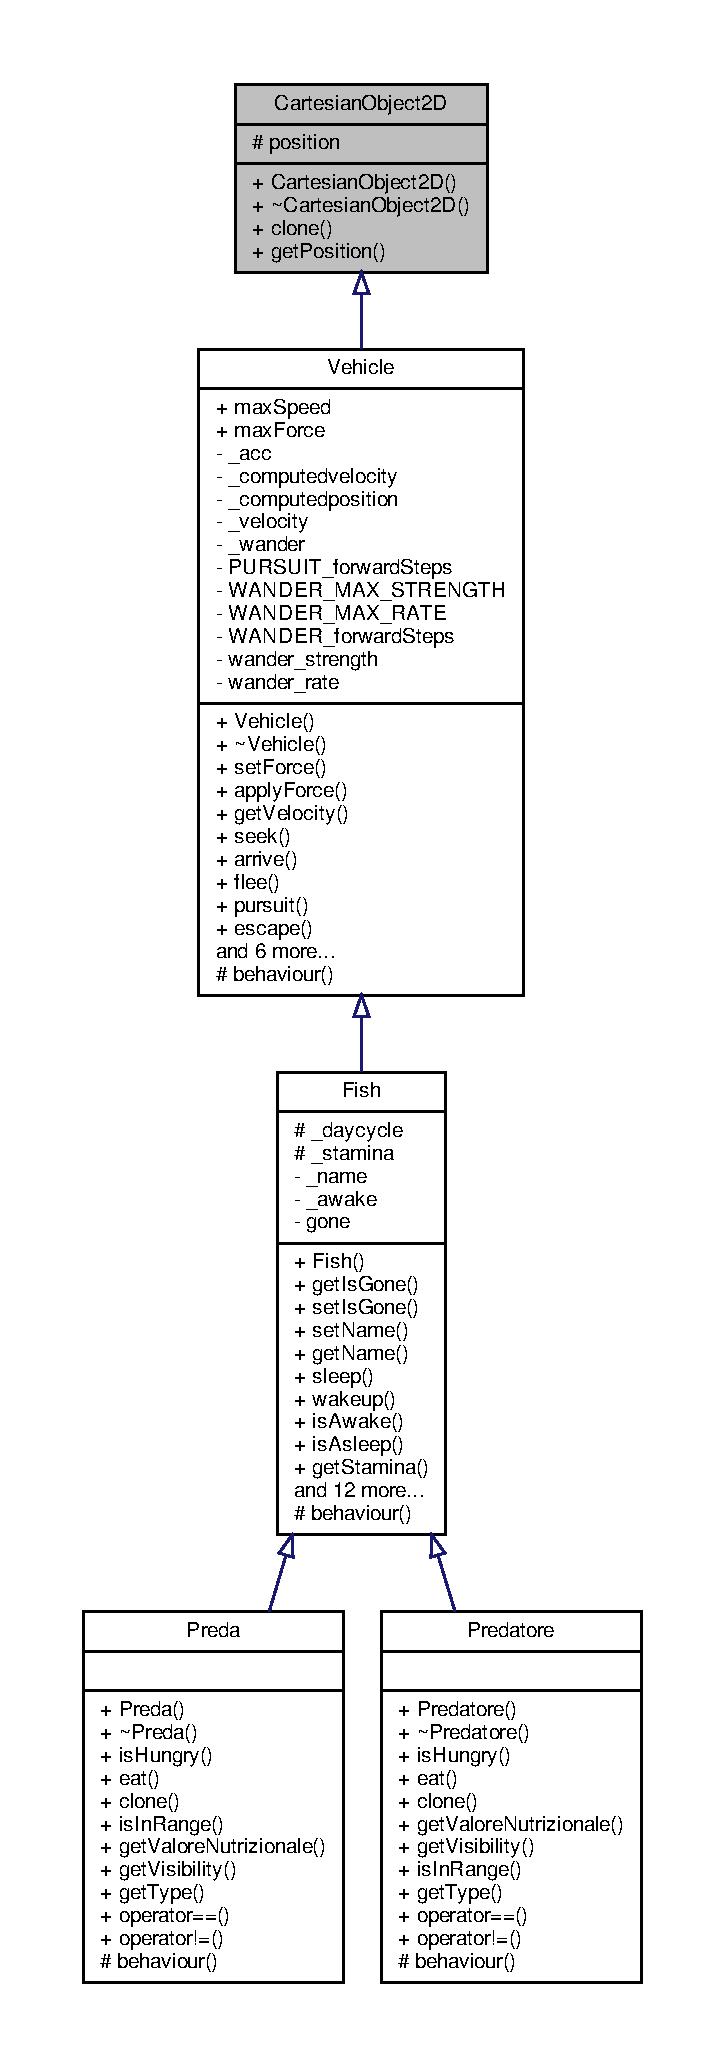
\includegraphics[height=550pt]{classCartesianObject2D__inherit__graph}
\end{center}
\end{figure}


Collaboration diagram for Cartesian\+Object2D\+:\nopagebreak
\begin{figure}[H]
\begin{center}
\leavevmode
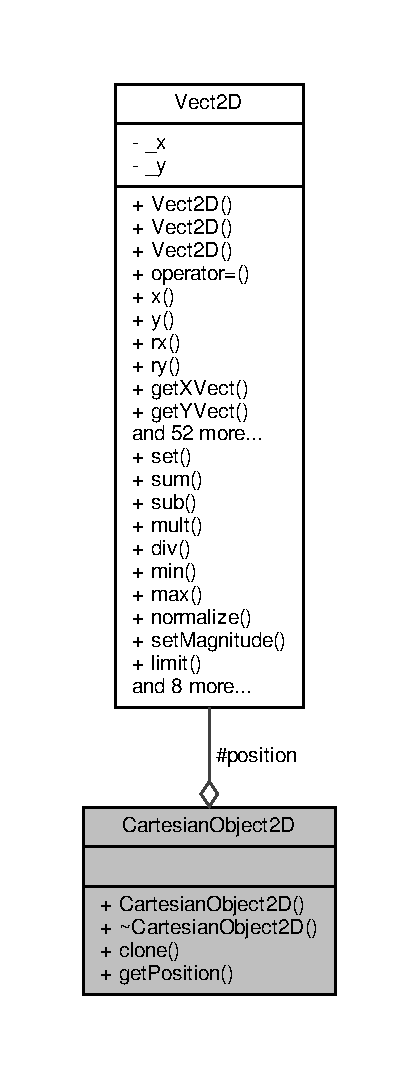
\includegraphics[width=201pt]{classCartesianObject2D__coll__graph}
\end{center}
\end{figure}
\subsection*{Public Member Functions}
\begin{DoxyCompactItemize}
\item 
\hyperlink{classCartesianObject2D_a4e32dae738f975ef1d323b2810fc0b72_a4e32dae738f975ef1d323b2810fc0b72}{Cartesian\+Object2D} (const \hyperlink{classVect2D}{Vect2D} \&p=\hyperlink{classVect2D}{Vect2D}(0, 0))
\item 
virtual \hyperlink{classCartesianObject2D_a16f2f813e178802ec316fcedae39f7af_a16f2f813e178802ec316fcedae39f7af}{$\sim$\+Cartesian\+Object2D} ()
\item 
virtual \hyperlink{classCartesianObject2D}{Cartesian\+Object2D} $\ast$ \hyperlink{classCartesianObject2D_afd883b92328b20defd9ed7af581206ab_afd883b92328b20defd9ed7af581206ab}{clone} () const =0
\item 
\hyperlink{classVect2D}{Vect2D} \hyperlink{classCartesianObject2D_aa3a6b63777852ab9eb9408ed2536abe2_aa3a6b63777852ab9eb9408ed2536abe2}{get\+Position} () const
\end{DoxyCompactItemize}
\subsection*{Protected Attributes}
\begin{DoxyCompactItemize}
\item 
\hyperlink{classVect2D}{Vect2D} \hyperlink{classCartesianObject2D_ae02ec6ed11f9bfc0c748da033d6a32f9_ae02ec6ed11f9bfc0c748da033d6a32f9}{position}
\end{DoxyCompactItemize}


\subsection{Constructor \& Destructor Documentation}
\mbox{\Hypertarget{classCartesianObject2D_a4e32dae738f975ef1d323b2810fc0b72_a4e32dae738f975ef1d323b2810fc0b72}\label{classCartesianObject2D_a4e32dae738f975ef1d323b2810fc0b72_a4e32dae738f975ef1d323b2810fc0b72}} 
\index{Cartesian\+Object2D@{Cartesian\+Object2D}!Cartesian\+Object2D@{Cartesian\+Object2D}}
\index{Cartesian\+Object2D@{Cartesian\+Object2D}!Cartesian\+Object2D@{Cartesian\+Object2D}}
\subsubsection{\texorpdfstring{Cartesian\+Object2\+D()}{CartesianObject2D()}}
{\footnotesize\ttfamily Cartesian\+Object2\+D\+::\+Cartesian\+Object2D (\begin{DoxyParamCaption}\item[{const \hyperlink{classVect2D}{Vect2D} \&}]{p = {\ttfamily \hyperlink{classVect2D}{Vect2D}(0,~0)} }\end{DoxyParamCaption})}

\mbox{\Hypertarget{classCartesianObject2D_a16f2f813e178802ec316fcedae39f7af_a16f2f813e178802ec316fcedae39f7af}\label{classCartesianObject2D_a16f2f813e178802ec316fcedae39f7af_a16f2f813e178802ec316fcedae39f7af}} 
\index{Cartesian\+Object2D@{Cartesian\+Object2D}!````~Cartesian\+Object2D@{$\sim$\+Cartesian\+Object2D}}
\index{````~Cartesian\+Object2D@{$\sim$\+Cartesian\+Object2D}!Cartesian\+Object2D@{Cartesian\+Object2D}}
\subsubsection{\texorpdfstring{$\sim$\+Cartesian\+Object2\+D()}{~CartesianObject2D()}}
{\footnotesize\ttfamily Cartesian\+Object2\+D\+::$\sim$\+Cartesian\+Object2D (\begin{DoxyParamCaption}{ }\end{DoxyParamCaption})\hspace{0.3cm}{\ttfamily [virtual]}}



\subsection{Member Function Documentation}
\mbox{\Hypertarget{classCartesianObject2D_afd883b92328b20defd9ed7af581206ab_afd883b92328b20defd9ed7af581206ab}\label{classCartesianObject2D_afd883b92328b20defd9ed7af581206ab_afd883b92328b20defd9ed7af581206ab}} 
\index{Cartesian\+Object2D@{Cartesian\+Object2D}!clone@{clone}}
\index{clone@{clone}!Cartesian\+Object2D@{Cartesian\+Object2D}}
\subsubsection{\texorpdfstring{clone()}{clone()}}
{\footnotesize\ttfamily virtual \hyperlink{classCartesianObject2D}{Cartesian\+Object2D}$\ast$ Cartesian\+Object2\+D\+::clone (\begin{DoxyParamCaption}{ }\end{DoxyParamCaption}) const\hspace{0.3cm}{\ttfamily [pure virtual]}}



Implemented in \hyperlink{classVehicle_a6c8513134608499d188a2e994accdb7c_a6c8513134608499d188a2e994accdb7c}{Vehicle}, \hyperlink{classFish_a6732945f7373a28b1723e55de8a65e13_a6732945f7373a28b1723e55de8a65e13}{Fish}, \hyperlink{classPredatore_a493b41e7df1542c10cdd646559514917_a493b41e7df1542c10cdd646559514917}{Predatore}, and \hyperlink{classPreda_a12baf94e52873bf3b9a9a9da84c357c5_a12baf94e52873bf3b9a9a9da84c357c5}{Preda}.

\mbox{\Hypertarget{classCartesianObject2D_aa3a6b63777852ab9eb9408ed2536abe2_aa3a6b63777852ab9eb9408ed2536abe2}\label{classCartesianObject2D_aa3a6b63777852ab9eb9408ed2536abe2_aa3a6b63777852ab9eb9408ed2536abe2}} 
\index{Cartesian\+Object2D@{Cartesian\+Object2D}!get\+Position@{get\+Position}}
\index{get\+Position@{get\+Position}!Cartesian\+Object2D@{Cartesian\+Object2D}}
\subsubsection{\texorpdfstring{get\+Position()}{getPosition()}}
{\footnotesize\ttfamily \hyperlink{classVect2D}{Vect2D} Cartesian\+Object2\+D\+::get\+Position (\begin{DoxyParamCaption}{ }\end{DoxyParamCaption}) const}



\subsection{Member Data Documentation}
\mbox{\Hypertarget{classCartesianObject2D_ae02ec6ed11f9bfc0c748da033d6a32f9_ae02ec6ed11f9bfc0c748da033d6a32f9}\label{classCartesianObject2D_ae02ec6ed11f9bfc0c748da033d6a32f9_ae02ec6ed11f9bfc0c748da033d6a32f9}} 
\index{Cartesian\+Object2D@{Cartesian\+Object2D}!position@{position}}
\index{position@{position}!Cartesian\+Object2D@{Cartesian\+Object2D}}
\subsubsection{\texorpdfstring{position}{position}}
{\footnotesize\ttfamily \hyperlink{classVect2D}{Vect2D} Cartesian\+Object2\+D\+::position\hspace{0.3cm}{\ttfamily [protected]}}



The documentation for this class was generated from the following files\+:\begin{DoxyCompactItemize}
\item 
include/\hyperlink{cartesianobject2d_8hpp}{cartesianobject2d.\+hpp}\item 
src/\hyperlink{cartesianobject2d_8cpp}{cartesianobject2d.\+cpp}\end{DoxyCompactItemize}

\hypertarget{classVector_1_1const__iterator}{}\section{Vector$<$ T $>$\+:\+:const\+\_\+iterator Class Reference}
\label{classVector_1_1const__iterator}\index{Vector$<$ T $>$\+::const\+\_\+iterator@{Vector$<$ T $>$\+::const\+\_\+iterator}}


{\ttfamily \#include $<$vector.\+hpp$>$}



Collaboration diagram for Vector$<$ T $>$\+:\+:const\+\_\+iterator\+:\nopagebreak
\begin{figure}[H]
\begin{center}
\leavevmode
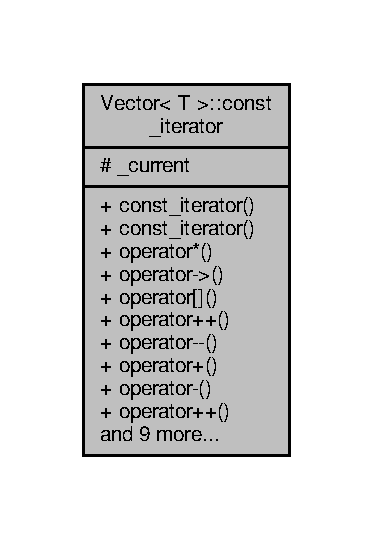
\includegraphics[width=179pt]{classVector_1_1const__iterator__coll__graph}
\end{center}
\end{figure}
\subsection*{Public Member Functions}
\begin{DoxyCompactItemize}
\item 
\hyperlink{classVector_1_1const__iterator_afa2f13d4f57db06cc18b08d1250108de_afa2f13d4f57db06cc18b08d1250108de}{const\+\_\+iterator} (T $\ast$i=nullptr)
\item 
\hyperlink{classVector_1_1const__iterator_ab513d0d4c5a9f0d66b8300bb39e762be_ab513d0d4c5a9f0d66b8300bb39e762be}{const\+\_\+iterator} (const \hyperlink{classVector_1_1const__iterator}{const\+\_\+iterator} \&i)
\item 
const T \& \hyperlink{classVector_1_1const__iterator_ad93bad8edb6d08eaf7685bd91aea15e5_ad93bad8edb6d08eaf7685bd91aea15e5}{operator$\ast$} () const
\item 
const T $\ast$ \hyperlink{classVector_1_1const__iterator_a627fd21e373252cc9f07620cef64b426_a627fd21e373252cc9f07620cef64b426}{operator-\/$>$} () const
\item 
const T \& \hyperlink{classVector_1_1const__iterator_a595b0bd316e5e6155a56391d41952f22_a595b0bd316e5e6155a56391d41952f22}{operator\mbox{[}$\,$\mbox{]}} (int n) const
\item 
\hyperlink{classVector_1_1const__iterator}{const\+\_\+iterator} \hyperlink{classVector_1_1const__iterator_a67456e47c6bd9b973893d4c367dc6a46_a67456e47c6bd9b973893d4c367dc6a46}{operator++} (int)
\item 
\hyperlink{classVector_1_1const__iterator}{const\+\_\+iterator} \hyperlink{classVector_1_1const__iterator_ab402f46148c6b50a3b967165403912c9_ab402f46148c6b50a3b967165403912c9}{operator-\/-\/} (int)
\item 
\hyperlink{classVector_1_1const__iterator}{const\+\_\+iterator} \hyperlink{classVector_1_1const__iterator_a6b3e3a9f4a0f6817446fc7e0bad4f59c_a6b3e3a9f4a0f6817446fc7e0bad4f59c}{operator+} (int n) const
\item 
\hyperlink{classVector_1_1const__iterator}{const\+\_\+iterator} \hyperlink{classVector_1_1const__iterator_aff6f8ecfef16090d21113ca1bbf77a3c_aff6f8ecfef16090d21113ca1bbf77a3c}{operator-\/} (int n) const
\item 
\hyperlink{classVector_1_1const__iterator}{const\+\_\+iterator} \& \hyperlink{classVector_1_1const__iterator_a2f031ab9801a4c42de40b95b855bacd6_a2f031ab9801a4c42de40b95b855bacd6}{operator++} ()
\item 
\hyperlink{classVector_1_1const__iterator}{const\+\_\+iterator} \& \hyperlink{classVector_1_1const__iterator_a1040c4e1ecb2780da4a94449eef6690f_a1040c4e1ecb2780da4a94449eef6690f}{operator-\/-\/} ()
\item 
\hyperlink{classVector_1_1const__iterator}{const\+\_\+iterator} \& \hyperlink{classVector_1_1const__iterator_a0adddda02db5aace233912940c8f8979_a0adddda02db5aace233912940c8f8979}{operator+=} (int n)
\item 
\hyperlink{classVector_1_1const__iterator}{const\+\_\+iterator} \& \hyperlink{classVector_1_1const__iterator_af223a63e9a0587781de597ef50f3b7db_af223a63e9a0587781de597ef50f3b7db}{operator-\/=} (int n)
\item 
bool \hyperlink{classVector_1_1const__iterator_a6bd4b35ce30423fa93de1109fac60efd_a6bd4b35ce30423fa93de1109fac60efd}{operator==} (const \hyperlink{classVector_1_1const__iterator}{const\+\_\+iterator} \&i) const
\item 
bool \hyperlink{classVector_1_1const__iterator_a18870100713906a04755d7269665a1ed_a18870100713906a04755d7269665a1ed}{operator!=} (const \hyperlink{classVector_1_1const__iterator}{const\+\_\+iterator} \&i) const
\item 
bool \hyperlink{classVector_1_1const__iterator_a88a32fe91bda0079a2f7da6f07171ca2_a88a32fe91bda0079a2f7da6f07171ca2}{operator$<$} (const \hyperlink{classVector_1_1const__iterator}{const\+\_\+iterator} \&i) const
\item 
bool \hyperlink{classVector_1_1const__iterator_af5064ab82341e26c1518b228acc0f824_af5064ab82341e26c1518b228acc0f824}{operator$>$} (const \hyperlink{classVector_1_1const__iterator}{const\+\_\+iterator} \&i) const
\item 
bool \hyperlink{classVector_1_1const__iterator_af0cd8adfd475f12608d743dc2ec6624f_af0cd8adfd475f12608d743dc2ec6624f}{operator$<$=} (const \hyperlink{classVector_1_1const__iterator}{const\+\_\+iterator} \&i) const
\item 
bool \hyperlink{classVector_1_1const__iterator_a353332912e5cdc2c95339bd9f2735ee7_a353332912e5cdc2c95339bd9f2735ee7}{operator$>$=} (const \hyperlink{classVector_1_1const__iterator}{const\+\_\+iterator} \&i) const
\end{DoxyCompactItemize}
\subsection*{Protected Attributes}
\begin{DoxyCompactItemize}
\item 
T $\ast$ \hyperlink{classVector_1_1const__iterator_aad73aad5797a6ff013553310ee35b7cd_aad73aad5797a6ff013553310ee35b7cd}{\+\_\+current}
\end{DoxyCompactItemize}


\subsection{Constructor \& Destructor Documentation}
\mbox{\Hypertarget{classVector_1_1const__iterator_afa2f13d4f57db06cc18b08d1250108de_afa2f13d4f57db06cc18b08d1250108de}\label{classVector_1_1const__iterator_afa2f13d4f57db06cc18b08d1250108de_afa2f13d4f57db06cc18b08d1250108de}} 
\index{Vector\+::const\+\_\+iterator@{Vector\+::const\+\_\+iterator}!const\+\_\+iterator@{const\+\_\+iterator}}
\index{const\+\_\+iterator@{const\+\_\+iterator}!Vector\+::const\+\_\+iterator@{Vector\+::const\+\_\+iterator}}
\subsubsection{\texorpdfstring{const\+\_\+iterator()}{const\_iterator()}\hspace{0.1cm}{\footnotesize\ttfamily [1/2]}}
{\footnotesize\ttfamily template$<$class T$>$ \\
\hyperlink{classVector}{Vector}$<$ T $>$\+::const\+\_\+iterator\+::const\+\_\+iterator (\begin{DoxyParamCaption}\item[{T $\ast$}]{i = {\ttfamily nullptr} }\end{DoxyParamCaption})\hspace{0.3cm}{\ttfamily [inline]}}

\mbox{\Hypertarget{classVector_1_1const__iterator_ab513d0d4c5a9f0d66b8300bb39e762be_ab513d0d4c5a9f0d66b8300bb39e762be}\label{classVector_1_1const__iterator_ab513d0d4c5a9f0d66b8300bb39e762be_ab513d0d4c5a9f0d66b8300bb39e762be}} 
\index{Vector\+::const\+\_\+iterator@{Vector\+::const\+\_\+iterator}!const\+\_\+iterator@{const\+\_\+iterator}}
\index{const\+\_\+iterator@{const\+\_\+iterator}!Vector\+::const\+\_\+iterator@{Vector\+::const\+\_\+iterator}}
\subsubsection{\texorpdfstring{const\+\_\+iterator()}{const\_iterator()}\hspace{0.1cm}{\footnotesize\ttfamily [2/2]}}
{\footnotesize\ttfamily template$<$class T$>$ \\
\hyperlink{classVector}{Vector}$<$ T $>$\+::const\+\_\+iterator\+::const\+\_\+iterator (\begin{DoxyParamCaption}\item[{const \hyperlink{classVector_1_1const__iterator}{const\+\_\+iterator} \&}]{i }\end{DoxyParamCaption})\hspace{0.3cm}{\ttfamily [inline]}}



\subsection{Member Function Documentation}
\mbox{\Hypertarget{classVector_1_1const__iterator_a18870100713906a04755d7269665a1ed_a18870100713906a04755d7269665a1ed}\label{classVector_1_1const__iterator_a18870100713906a04755d7269665a1ed_a18870100713906a04755d7269665a1ed}} 
\index{Vector\+::const\+\_\+iterator@{Vector\+::const\+\_\+iterator}!operator"!=@{operator"!=}}
\index{operator"!=@{operator"!=}!Vector\+::const\+\_\+iterator@{Vector\+::const\+\_\+iterator}}
\subsubsection{\texorpdfstring{operator"!=()}{operator!=()}}
{\footnotesize\ttfamily template$<$class T$>$ \\
bool \hyperlink{classVector}{Vector}$<$ T $>$\+::const\+\_\+iterator\+::operator!= (\begin{DoxyParamCaption}\item[{const \hyperlink{classVector_1_1const__iterator}{const\+\_\+iterator} \&}]{i }\end{DoxyParamCaption}) const\hspace{0.3cm}{\ttfamily [inline]}}

\mbox{\Hypertarget{classVector_1_1const__iterator_ad93bad8edb6d08eaf7685bd91aea15e5_ad93bad8edb6d08eaf7685bd91aea15e5}\label{classVector_1_1const__iterator_ad93bad8edb6d08eaf7685bd91aea15e5_ad93bad8edb6d08eaf7685bd91aea15e5}} 
\index{Vector\+::const\+\_\+iterator@{Vector\+::const\+\_\+iterator}!operator$\ast$@{operator$\ast$}}
\index{operator$\ast$@{operator$\ast$}!Vector\+::const\+\_\+iterator@{Vector\+::const\+\_\+iterator}}
\subsubsection{\texorpdfstring{operator$\ast$()}{operator*()}}
{\footnotesize\ttfamily template$<$class T$>$ \\
const T\& \hyperlink{classVector}{Vector}$<$ T $>$\+::const\+\_\+iterator\+::operator$\ast$ (\begin{DoxyParamCaption}{ }\end{DoxyParamCaption}) const\hspace{0.3cm}{\ttfamily [inline]}}

\mbox{\Hypertarget{classVector_1_1const__iterator_a6b3e3a9f4a0f6817446fc7e0bad4f59c_a6b3e3a9f4a0f6817446fc7e0bad4f59c}\label{classVector_1_1const__iterator_a6b3e3a9f4a0f6817446fc7e0bad4f59c_a6b3e3a9f4a0f6817446fc7e0bad4f59c}} 
\index{Vector\+::const\+\_\+iterator@{Vector\+::const\+\_\+iterator}!operator+@{operator+}}
\index{operator+@{operator+}!Vector\+::const\+\_\+iterator@{Vector\+::const\+\_\+iterator}}
\subsubsection{\texorpdfstring{operator+()}{operator+()}}
{\footnotesize\ttfamily template$<$class T$>$ \\
\hyperlink{classVector_1_1const__iterator}{const\+\_\+iterator} \hyperlink{classVector}{Vector}$<$ T $>$\+::const\+\_\+iterator\+::operator+ (\begin{DoxyParamCaption}\item[{int}]{n }\end{DoxyParamCaption}) const\hspace{0.3cm}{\ttfamily [inline]}}

\mbox{\Hypertarget{classVector_1_1const__iterator_a67456e47c6bd9b973893d4c367dc6a46_a67456e47c6bd9b973893d4c367dc6a46}\label{classVector_1_1const__iterator_a67456e47c6bd9b973893d4c367dc6a46_a67456e47c6bd9b973893d4c367dc6a46}} 
\index{Vector\+::const\+\_\+iterator@{Vector\+::const\+\_\+iterator}!operator++@{operator++}}
\index{operator++@{operator++}!Vector\+::const\+\_\+iterator@{Vector\+::const\+\_\+iterator}}
\subsubsection{\texorpdfstring{operator++()}{operator++()}\hspace{0.1cm}{\footnotesize\ttfamily [1/2]}}
{\footnotesize\ttfamily template$<$class T$>$ \\
\hyperlink{classVector_1_1const__iterator}{const\+\_\+iterator} \hyperlink{classVector}{Vector}$<$ T $>$\+::const\+\_\+iterator\+::operator++ (\begin{DoxyParamCaption}\item[{int}]{ }\end{DoxyParamCaption})\hspace{0.3cm}{\ttfamily [inline]}}

\mbox{\Hypertarget{classVector_1_1const__iterator_a2f031ab9801a4c42de40b95b855bacd6_a2f031ab9801a4c42de40b95b855bacd6}\label{classVector_1_1const__iterator_a2f031ab9801a4c42de40b95b855bacd6_a2f031ab9801a4c42de40b95b855bacd6}} 
\index{Vector\+::const\+\_\+iterator@{Vector\+::const\+\_\+iterator}!operator++@{operator++}}
\index{operator++@{operator++}!Vector\+::const\+\_\+iterator@{Vector\+::const\+\_\+iterator}}
\subsubsection{\texorpdfstring{operator++()}{operator++()}\hspace{0.1cm}{\footnotesize\ttfamily [2/2]}}
{\footnotesize\ttfamily template$<$class T$>$ \\
\hyperlink{classVector_1_1const__iterator}{const\+\_\+iterator}\& \hyperlink{classVector}{Vector}$<$ T $>$\+::const\+\_\+iterator\+::operator++ (\begin{DoxyParamCaption}{ }\end{DoxyParamCaption})\hspace{0.3cm}{\ttfamily [inline]}}

\mbox{\Hypertarget{classVector_1_1const__iterator_a0adddda02db5aace233912940c8f8979_a0adddda02db5aace233912940c8f8979}\label{classVector_1_1const__iterator_a0adddda02db5aace233912940c8f8979_a0adddda02db5aace233912940c8f8979}} 
\index{Vector\+::const\+\_\+iterator@{Vector\+::const\+\_\+iterator}!operator+=@{operator+=}}
\index{operator+=@{operator+=}!Vector\+::const\+\_\+iterator@{Vector\+::const\+\_\+iterator}}
\subsubsection{\texorpdfstring{operator+=()}{operator+=()}}
{\footnotesize\ttfamily template$<$class T$>$ \\
\hyperlink{classVector_1_1const__iterator}{const\+\_\+iterator}\& \hyperlink{classVector}{Vector}$<$ T $>$\+::const\+\_\+iterator\+::operator+= (\begin{DoxyParamCaption}\item[{int}]{n }\end{DoxyParamCaption})\hspace{0.3cm}{\ttfamily [inline]}}

\mbox{\Hypertarget{classVector_1_1const__iterator_aff6f8ecfef16090d21113ca1bbf77a3c_aff6f8ecfef16090d21113ca1bbf77a3c}\label{classVector_1_1const__iterator_aff6f8ecfef16090d21113ca1bbf77a3c_aff6f8ecfef16090d21113ca1bbf77a3c}} 
\index{Vector\+::const\+\_\+iterator@{Vector\+::const\+\_\+iterator}!operator-\/@{operator-\/}}
\index{operator-\/@{operator-\/}!Vector\+::const\+\_\+iterator@{Vector\+::const\+\_\+iterator}}
\subsubsection{\texorpdfstring{operator-\/()}{operator-()}}
{\footnotesize\ttfamily template$<$class T$>$ \\
\hyperlink{classVector_1_1const__iterator}{const\+\_\+iterator} \hyperlink{classVector}{Vector}$<$ T $>$\+::const\+\_\+iterator\+::operator-\/ (\begin{DoxyParamCaption}\item[{int}]{n }\end{DoxyParamCaption}) const\hspace{0.3cm}{\ttfamily [inline]}}

\mbox{\Hypertarget{classVector_1_1const__iterator_ab402f46148c6b50a3b967165403912c9_ab402f46148c6b50a3b967165403912c9}\label{classVector_1_1const__iterator_ab402f46148c6b50a3b967165403912c9_ab402f46148c6b50a3b967165403912c9}} 
\index{Vector\+::const\+\_\+iterator@{Vector\+::const\+\_\+iterator}!operator-\/-\/@{operator-\/-\/}}
\index{operator-\/-\/@{operator-\/-\/}!Vector\+::const\+\_\+iterator@{Vector\+::const\+\_\+iterator}}
\subsubsection{\texorpdfstring{operator-\/-\/()}{operator--()}\hspace{0.1cm}{\footnotesize\ttfamily [1/2]}}
{\footnotesize\ttfamily template$<$class T$>$ \\
\hyperlink{classVector_1_1const__iterator}{const\+\_\+iterator} \hyperlink{classVector}{Vector}$<$ T $>$\+::const\+\_\+iterator\+::operator-\/-\/ (\begin{DoxyParamCaption}\item[{int}]{ }\end{DoxyParamCaption})\hspace{0.3cm}{\ttfamily [inline]}}

\mbox{\Hypertarget{classVector_1_1const__iterator_a1040c4e1ecb2780da4a94449eef6690f_a1040c4e1ecb2780da4a94449eef6690f}\label{classVector_1_1const__iterator_a1040c4e1ecb2780da4a94449eef6690f_a1040c4e1ecb2780da4a94449eef6690f}} 
\index{Vector\+::const\+\_\+iterator@{Vector\+::const\+\_\+iterator}!operator-\/-\/@{operator-\/-\/}}
\index{operator-\/-\/@{operator-\/-\/}!Vector\+::const\+\_\+iterator@{Vector\+::const\+\_\+iterator}}
\subsubsection{\texorpdfstring{operator-\/-\/()}{operator--()}\hspace{0.1cm}{\footnotesize\ttfamily [2/2]}}
{\footnotesize\ttfamily template$<$class T$>$ \\
\hyperlink{classVector_1_1const__iterator}{const\+\_\+iterator}\& \hyperlink{classVector}{Vector}$<$ T $>$\+::const\+\_\+iterator\+::operator-\/-\/ (\begin{DoxyParamCaption}{ }\end{DoxyParamCaption})\hspace{0.3cm}{\ttfamily [inline]}}

\mbox{\Hypertarget{classVector_1_1const__iterator_af223a63e9a0587781de597ef50f3b7db_af223a63e9a0587781de597ef50f3b7db}\label{classVector_1_1const__iterator_af223a63e9a0587781de597ef50f3b7db_af223a63e9a0587781de597ef50f3b7db}} 
\index{Vector\+::const\+\_\+iterator@{Vector\+::const\+\_\+iterator}!operator-\/=@{operator-\/=}}
\index{operator-\/=@{operator-\/=}!Vector\+::const\+\_\+iterator@{Vector\+::const\+\_\+iterator}}
\subsubsection{\texorpdfstring{operator-\/=()}{operator-=()}}
{\footnotesize\ttfamily template$<$class T$>$ \\
\hyperlink{classVector_1_1const__iterator}{const\+\_\+iterator}\& \hyperlink{classVector}{Vector}$<$ T $>$\+::const\+\_\+iterator\+::operator-\/= (\begin{DoxyParamCaption}\item[{int}]{n }\end{DoxyParamCaption})\hspace{0.3cm}{\ttfamily [inline]}}

\mbox{\Hypertarget{classVector_1_1const__iterator_a627fd21e373252cc9f07620cef64b426_a627fd21e373252cc9f07620cef64b426}\label{classVector_1_1const__iterator_a627fd21e373252cc9f07620cef64b426_a627fd21e373252cc9f07620cef64b426}} 
\index{Vector\+::const\+\_\+iterator@{Vector\+::const\+\_\+iterator}!operator-\/$>$@{operator-\/$>$}}
\index{operator-\/$>$@{operator-\/$>$}!Vector\+::const\+\_\+iterator@{Vector\+::const\+\_\+iterator}}
\subsubsection{\texorpdfstring{operator-\/$>$()}{operator->()}}
{\footnotesize\ttfamily template$<$class T$>$ \\
const T$\ast$ \hyperlink{classVector}{Vector}$<$ T $>$\+::const\+\_\+iterator\+::operator-\/$>$ (\begin{DoxyParamCaption}{ }\end{DoxyParamCaption}) const\hspace{0.3cm}{\ttfamily [inline]}}

\mbox{\Hypertarget{classVector_1_1const__iterator_a88a32fe91bda0079a2f7da6f07171ca2_a88a32fe91bda0079a2f7da6f07171ca2}\label{classVector_1_1const__iterator_a88a32fe91bda0079a2f7da6f07171ca2_a88a32fe91bda0079a2f7da6f07171ca2}} 
\index{Vector\+::const\+\_\+iterator@{Vector\+::const\+\_\+iterator}!operator$<$@{operator$<$}}
\index{operator$<$@{operator$<$}!Vector\+::const\+\_\+iterator@{Vector\+::const\+\_\+iterator}}
\subsubsection{\texorpdfstring{operator$<$()}{operator<()}}
{\footnotesize\ttfamily template$<$class T$>$ \\
bool \hyperlink{classVector}{Vector}$<$ T $>$\+::const\+\_\+iterator\+::operator$<$ (\begin{DoxyParamCaption}\item[{const \hyperlink{classVector_1_1const__iterator}{const\+\_\+iterator} \&}]{i }\end{DoxyParamCaption}) const\hspace{0.3cm}{\ttfamily [inline]}}

\mbox{\Hypertarget{classVector_1_1const__iterator_af0cd8adfd475f12608d743dc2ec6624f_af0cd8adfd475f12608d743dc2ec6624f}\label{classVector_1_1const__iterator_af0cd8adfd475f12608d743dc2ec6624f_af0cd8adfd475f12608d743dc2ec6624f}} 
\index{Vector\+::const\+\_\+iterator@{Vector\+::const\+\_\+iterator}!operator$<$=@{operator$<$=}}
\index{operator$<$=@{operator$<$=}!Vector\+::const\+\_\+iterator@{Vector\+::const\+\_\+iterator}}
\subsubsection{\texorpdfstring{operator$<$=()}{operator<=()}}
{\footnotesize\ttfamily template$<$class T$>$ \\
bool \hyperlink{classVector}{Vector}$<$ T $>$\+::const\+\_\+iterator\+::operator$<$= (\begin{DoxyParamCaption}\item[{const \hyperlink{classVector_1_1const__iterator}{const\+\_\+iterator} \&}]{i }\end{DoxyParamCaption}) const\hspace{0.3cm}{\ttfamily [inline]}}

\mbox{\Hypertarget{classVector_1_1const__iterator_a6bd4b35ce30423fa93de1109fac60efd_a6bd4b35ce30423fa93de1109fac60efd}\label{classVector_1_1const__iterator_a6bd4b35ce30423fa93de1109fac60efd_a6bd4b35ce30423fa93de1109fac60efd}} 
\index{Vector\+::const\+\_\+iterator@{Vector\+::const\+\_\+iterator}!operator==@{operator==}}
\index{operator==@{operator==}!Vector\+::const\+\_\+iterator@{Vector\+::const\+\_\+iterator}}
\subsubsection{\texorpdfstring{operator==()}{operator==()}}
{\footnotesize\ttfamily template$<$class T$>$ \\
bool \hyperlink{classVector}{Vector}$<$ T $>$\+::const\+\_\+iterator\+::operator== (\begin{DoxyParamCaption}\item[{const \hyperlink{classVector_1_1const__iterator}{const\+\_\+iterator} \&}]{i }\end{DoxyParamCaption}) const\hspace{0.3cm}{\ttfamily [inline]}}

\mbox{\Hypertarget{classVector_1_1const__iterator_af5064ab82341e26c1518b228acc0f824_af5064ab82341e26c1518b228acc0f824}\label{classVector_1_1const__iterator_af5064ab82341e26c1518b228acc0f824_af5064ab82341e26c1518b228acc0f824}} 
\index{Vector\+::const\+\_\+iterator@{Vector\+::const\+\_\+iterator}!operator$>$@{operator$>$}}
\index{operator$>$@{operator$>$}!Vector\+::const\+\_\+iterator@{Vector\+::const\+\_\+iterator}}
\subsubsection{\texorpdfstring{operator$>$()}{operator>()}}
{\footnotesize\ttfamily template$<$class T$>$ \\
bool \hyperlink{classVector}{Vector}$<$ T $>$\+::const\+\_\+iterator\+::operator$>$ (\begin{DoxyParamCaption}\item[{const \hyperlink{classVector_1_1const__iterator}{const\+\_\+iterator} \&}]{i }\end{DoxyParamCaption}) const\hspace{0.3cm}{\ttfamily [inline]}}

\mbox{\Hypertarget{classVector_1_1const__iterator_a353332912e5cdc2c95339bd9f2735ee7_a353332912e5cdc2c95339bd9f2735ee7}\label{classVector_1_1const__iterator_a353332912e5cdc2c95339bd9f2735ee7_a353332912e5cdc2c95339bd9f2735ee7}} 
\index{Vector\+::const\+\_\+iterator@{Vector\+::const\+\_\+iterator}!operator$>$=@{operator$>$=}}
\index{operator$>$=@{operator$>$=}!Vector\+::const\+\_\+iterator@{Vector\+::const\+\_\+iterator}}
\subsubsection{\texorpdfstring{operator$>$=()}{operator>=()}}
{\footnotesize\ttfamily template$<$class T$>$ \\
bool \hyperlink{classVector}{Vector}$<$ T $>$\+::const\+\_\+iterator\+::operator$>$= (\begin{DoxyParamCaption}\item[{const \hyperlink{classVector_1_1const__iterator}{const\+\_\+iterator} \&}]{i }\end{DoxyParamCaption}) const\hspace{0.3cm}{\ttfamily [inline]}}

\mbox{\Hypertarget{classVector_1_1const__iterator_a595b0bd316e5e6155a56391d41952f22_a595b0bd316e5e6155a56391d41952f22}\label{classVector_1_1const__iterator_a595b0bd316e5e6155a56391d41952f22_a595b0bd316e5e6155a56391d41952f22}} 
\index{Vector\+::const\+\_\+iterator@{Vector\+::const\+\_\+iterator}!operator\mbox{[}\mbox{]}@{operator[]}}
\index{operator\mbox{[}\mbox{]}@{operator[]}!Vector\+::const\+\_\+iterator@{Vector\+::const\+\_\+iterator}}
\subsubsection{\texorpdfstring{operator[]()}{operator[]()}}
{\footnotesize\ttfamily template$<$class T$>$ \\
const T\& \hyperlink{classVector}{Vector}$<$ T $>$\+::const\+\_\+iterator\+::operator\mbox{[}$\,$\mbox{]} (\begin{DoxyParamCaption}\item[{int}]{n }\end{DoxyParamCaption}) const\hspace{0.3cm}{\ttfamily [inline]}}



\subsection{Member Data Documentation}
\mbox{\Hypertarget{classVector_1_1const__iterator_aad73aad5797a6ff013553310ee35b7cd_aad73aad5797a6ff013553310ee35b7cd}\label{classVector_1_1const__iterator_aad73aad5797a6ff013553310ee35b7cd_aad73aad5797a6ff013553310ee35b7cd}} 
\index{Vector\+::const\+\_\+iterator@{Vector\+::const\+\_\+iterator}!\+\_\+current@{\+\_\+current}}
\index{\+\_\+current@{\+\_\+current}!Vector\+::const\+\_\+iterator@{Vector\+::const\+\_\+iterator}}
\subsubsection{\texorpdfstring{\+\_\+current}{\_current}}
{\footnotesize\ttfamily template$<$class T$>$ \\
T$\ast$ \hyperlink{classVector}{Vector}$<$ T $>$\+::const\+\_\+iterator\+::\+\_\+current\hspace{0.3cm}{\ttfamily [protected]}}



The documentation for this class was generated from the following file\+:\begin{DoxyCompactItemize}
\item 
include/\hyperlink{vector_8hpp}{vector.\+hpp}\end{DoxyCompactItemize}

\hypertarget{classController}{}\section{Controller Class Reference}
\label{classController}\index{Controller@{Controller}}


{\ttfamily \#include $<$controller.\+hpp$>$}



Inheritance diagram for Controller\+:\nopagebreak
\begin{figure}[H]
\begin{center}
\leavevmode
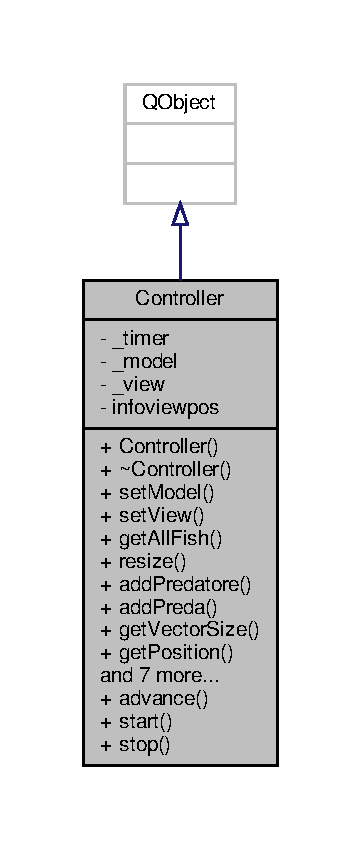
\includegraphics[width=173pt]{classController__inherit__graph}
\end{center}
\end{figure}


Collaboration diagram for Controller\+:\nopagebreak
\begin{figure}[H]
\begin{center}
\leavevmode
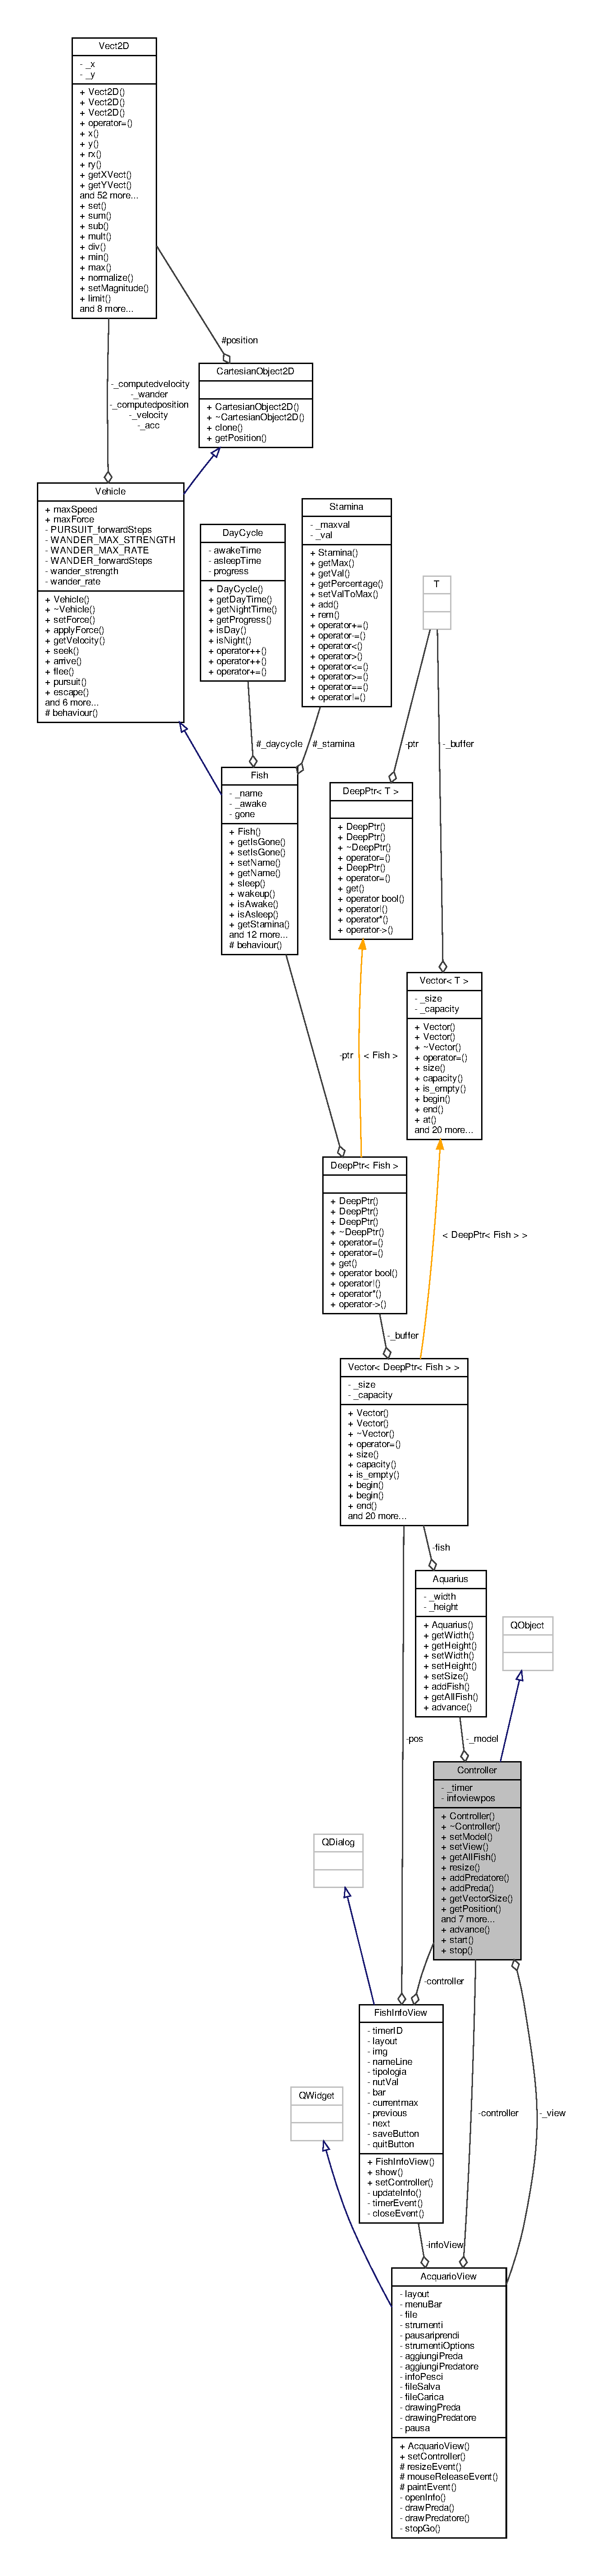
\includegraphics[height=550pt]{classController__coll__graph}
\end{center}
\end{figure}
\subsection*{Public Slots}
\begin{DoxyCompactItemize}
\item 
void \hyperlink{classController_a6d5730d65fa4c51130b9595ebf075437_a6d5730d65fa4c51130b9595ebf075437}{advance} ()
\item 
void \hyperlink{classController_ad535ad74055e645b7f44b7feeb4e82a8_ad535ad74055e645b7f44b7feeb4e82a8}{start} ()
\item 
void \hyperlink{classController_ad2abd6ee544cb1cb39705f31c6700f0c_ad2abd6ee544cb1cb39705f31c6700f0c}{stop} ()
\end{DoxyCompactItemize}
\subsection*{Public Member Functions}
\begin{DoxyCompactItemize}
\item 
\hyperlink{classController_af888a35f7a377692726d81332edf08ab_af888a35f7a377692726d81332edf08ab}{Controller} (Q\+Object $\ast$parent=nullptr)
\item 
\hyperlink{classController_a0ab87934c4f7a266cfdb86e0f36bc1b5_a0ab87934c4f7a266cfdb86e0f36bc1b5}{$\sim$\+Controller} ()
\item 
void \hyperlink{classController_a7506d17de939f6a84d3c057a55cf9272_a7506d17de939f6a84d3c057a55cf9272}{set\+Model} (\hyperlink{classAquarius}{Aquarius} $\ast$)
\item 
void \hyperlink{classController_a41aedc9fb5b715434c46097906aed910_a41aedc9fb5b715434c46097906aed910}{set\+View} (\hyperlink{classAcquarioView}{Acquario\+View} $\ast$)
\item 
\hyperlink{classVector}{Vector}$<$ \hyperlink{classDeepPtr}{Deep\+Ptr}$<$ \hyperlink{classFish}{Fish} $>$ $>$ \& \hyperlink{classController_aff25249a2b638e88e44d3c85c80f7ad6_aff25249a2b638e88e44d3c85c80f7ad6}{get\+All\+Fish} ()
\item 
void \hyperlink{classController_a9c71f8356f16cafffe3a878a58bd43e8_a9c71f8356f16cafffe3a878a58bd43e8}{resize} (int width, int height)
\item 
void \hyperlink{classController_a38346ab691e6d83dec69c3d60839d414_a38346ab691e6d83dec69c3d60839d414}{add\+Predatore} (const \hyperlink{classVect2D}{Vect2D} \&)
\item 
void \hyperlink{classController_ad1cbf75efaef06838c322c0d11deb473_ad1cbf75efaef06838c322c0d11deb473}{add\+Preda} (const \hyperlink{classVect2D}{Vect2D} \&)
\item 
unsigned int \hyperlink{classController_a3d9e63417c55b627ac7d79017f672617_a3d9e63417c55b627ac7d79017f672617}{get\+Vector\+Size} ()
\item 
unsigned int \hyperlink{classController_ade92370baade9b789d4b47e75c830076_ade92370baade9b789d4b47e75c830076}{get\+Position} ()
\item 
bool \hyperlink{classController_a2c4171f922bf604da9b1db2f9b2b4d15_a2c4171f922bf604da9b1db2f9b2b4d15}{has\+Next} ()
\item 
bool \hyperlink{classController_ab052ce96b259dc18a6b61506e678ca65_ab052ce96b259dc18a6b61506e678ca65}{has\+Prev} ()
\item 
void \hyperlink{classController_a2c820651428c830c576afdc9e322e61f_a2c820651428c830c576afdc9e322e61f}{next} ()
\item 
void \hyperlink{classController_a20b800af3abd4764264911ccf8eeb69e_a20b800af3abd4764264911ccf8eeb69e}{prev} ()
\item 
void \hyperlink{classController_ab5515748f1b0c82f015e039c817ee5f7_ab5515748f1b0c82f015e039c817ee5f7}{reset} ()
\item 
const \hyperlink{classFish}{Fish} $\ast$ \hyperlink{classController_a6689a578c69a6f2d08a59562e607a8c2_a6689a578c69a6f2d08a59562e607a8c2}{get\+Current} ()
\item 
void \hyperlink{classController_af3a40c18aa5bda6b842b361525391500_af3a40c18aa5bda6b842b361525391500}{update\+Name} (const std\+::string \&)
\end{DoxyCompactItemize}
\subsection*{Private Attributes}
\begin{DoxyCompactItemize}
\item 
Q\+Timer $\ast$ \hyperlink{classController_a17ee08bcd34becc157003361c5989400_a17ee08bcd34becc157003361c5989400}{\+\_\+timer}
\item 
\hyperlink{classAquarius}{Aquarius} $\ast$ \hyperlink{classController_a01f4c88c2a9b59ef6f9abf4f41351140_a01f4c88c2a9b59ef6f9abf4f41351140}{\+\_\+model}
\item 
\hyperlink{classAcquarioView}{Acquario\+View} $\ast$ \hyperlink{classController_a0b21753f4ca1740b9ff415a4e4606df3_a0b21753f4ca1740b9ff415a4e4606df3}{\+\_\+view}
\item 
unsigned int \hyperlink{classController_a956a159c2089d8ecda76278b7f57e859_a956a159c2089d8ecda76278b7f57e859}{infoviewpos}
\end{DoxyCompactItemize}


\subsection{Constructor \& Destructor Documentation}
\mbox{\Hypertarget{classController_af888a35f7a377692726d81332edf08ab_af888a35f7a377692726d81332edf08ab}\label{classController_af888a35f7a377692726d81332edf08ab_af888a35f7a377692726d81332edf08ab}} 
\index{Controller@{Controller}!Controller@{Controller}}
\index{Controller@{Controller}!Controller@{Controller}}
\subsubsection{\texorpdfstring{Controller()}{Controller()}}
{\footnotesize\ttfamily Controller\+::\+Controller (\begin{DoxyParamCaption}\item[{Q\+Object $\ast$}]{parent = {\ttfamily nullptr} }\end{DoxyParamCaption})\hspace{0.3cm}{\ttfamily [explicit]}}

\mbox{\Hypertarget{classController_a0ab87934c4f7a266cfdb86e0f36bc1b5_a0ab87934c4f7a266cfdb86e0f36bc1b5}\label{classController_a0ab87934c4f7a266cfdb86e0f36bc1b5_a0ab87934c4f7a266cfdb86e0f36bc1b5}} 
\index{Controller@{Controller}!````~Controller@{$\sim$\+Controller}}
\index{````~Controller@{$\sim$\+Controller}!Controller@{Controller}}
\subsubsection{\texorpdfstring{$\sim$\+Controller()}{~Controller()}}
{\footnotesize\ttfamily Controller\+::$\sim$\+Controller (\begin{DoxyParamCaption}{ }\end{DoxyParamCaption})}



\subsection{Member Function Documentation}
\mbox{\Hypertarget{classController_ad1cbf75efaef06838c322c0d11deb473_ad1cbf75efaef06838c322c0d11deb473}\label{classController_ad1cbf75efaef06838c322c0d11deb473_ad1cbf75efaef06838c322c0d11deb473}} 
\index{Controller@{Controller}!add\+Preda@{add\+Preda}}
\index{add\+Preda@{add\+Preda}!Controller@{Controller}}
\subsubsection{\texorpdfstring{add\+Preda()}{addPreda()}}
{\footnotesize\ttfamily void Controller\+::add\+Preda (\begin{DoxyParamCaption}\item[{const \hyperlink{classVect2D}{Vect2D} \&}]{position }\end{DoxyParamCaption})}

\mbox{\Hypertarget{classController_a38346ab691e6d83dec69c3d60839d414_a38346ab691e6d83dec69c3d60839d414}\label{classController_a38346ab691e6d83dec69c3d60839d414_a38346ab691e6d83dec69c3d60839d414}} 
\index{Controller@{Controller}!add\+Predatore@{add\+Predatore}}
\index{add\+Predatore@{add\+Predatore}!Controller@{Controller}}
\subsubsection{\texorpdfstring{add\+Predatore()}{addPredatore()}}
{\footnotesize\ttfamily void Controller\+::add\+Predatore (\begin{DoxyParamCaption}\item[{const \hyperlink{classVect2D}{Vect2D} \&}]{position }\end{DoxyParamCaption})}

\mbox{\Hypertarget{classController_a6d5730d65fa4c51130b9595ebf075437_a6d5730d65fa4c51130b9595ebf075437}\label{classController_a6d5730d65fa4c51130b9595ebf075437_a6d5730d65fa4c51130b9595ebf075437}} 
\index{Controller@{Controller}!advance@{advance}}
\index{advance@{advance}!Controller@{Controller}}
\subsubsection{\texorpdfstring{advance}{advance}}
{\footnotesize\ttfamily void Controller\+::advance (\begin{DoxyParamCaption}{ }\end{DoxyParamCaption})\hspace{0.3cm}{\ttfamily [slot]}}

\mbox{\Hypertarget{classController_aff25249a2b638e88e44d3c85c80f7ad6_aff25249a2b638e88e44d3c85c80f7ad6}\label{classController_aff25249a2b638e88e44d3c85c80f7ad6_aff25249a2b638e88e44d3c85c80f7ad6}} 
\index{Controller@{Controller}!get\+All\+Fish@{get\+All\+Fish}}
\index{get\+All\+Fish@{get\+All\+Fish}!Controller@{Controller}}
\subsubsection{\texorpdfstring{get\+All\+Fish()}{getAllFish()}}
{\footnotesize\ttfamily \hyperlink{classVector}{Vector}$<$ \hyperlink{classDeepPtr}{Deep\+Ptr}$<$ \hyperlink{classFish}{Fish} $>$ $>$ \& Controller\+::get\+All\+Fish (\begin{DoxyParamCaption}{ }\end{DoxyParamCaption})}

\mbox{\Hypertarget{classController_a6689a578c69a6f2d08a59562e607a8c2_a6689a578c69a6f2d08a59562e607a8c2}\label{classController_a6689a578c69a6f2d08a59562e607a8c2_a6689a578c69a6f2d08a59562e607a8c2}} 
\index{Controller@{Controller}!get\+Current@{get\+Current}}
\index{get\+Current@{get\+Current}!Controller@{Controller}}
\subsubsection{\texorpdfstring{get\+Current()}{getCurrent()}}
{\footnotesize\ttfamily const \hyperlink{classFish}{Fish} $\ast$ Controller\+::get\+Current (\begin{DoxyParamCaption}{ }\end{DoxyParamCaption})}

\mbox{\Hypertarget{classController_ade92370baade9b789d4b47e75c830076_ade92370baade9b789d4b47e75c830076}\label{classController_ade92370baade9b789d4b47e75c830076_ade92370baade9b789d4b47e75c830076}} 
\index{Controller@{Controller}!get\+Position@{get\+Position}}
\index{get\+Position@{get\+Position}!Controller@{Controller}}
\subsubsection{\texorpdfstring{get\+Position()}{getPosition()}}
{\footnotesize\ttfamily unsigned int Controller\+::get\+Position (\begin{DoxyParamCaption}{ }\end{DoxyParamCaption})}

\mbox{\Hypertarget{classController_a3d9e63417c55b627ac7d79017f672617_a3d9e63417c55b627ac7d79017f672617}\label{classController_a3d9e63417c55b627ac7d79017f672617_a3d9e63417c55b627ac7d79017f672617}} 
\index{Controller@{Controller}!get\+Vector\+Size@{get\+Vector\+Size}}
\index{get\+Vector\+Size@{get\+Vector\+Size}!Controller@{Controller}}
\subsubsection{\texorpdfstring{get\+Vector\+Size()}{getVectorSize()}}
{\footnotesize\ttfamily unsigned int Controller\+::get\+Vector\+Size (\begin{DoxyParamCaption}{ }\end{DoxyParamCaption})}

\mbox{\Hypertarget{classController_a2c4171f922bf604da9b1db2f9b2b4d15_a2c4171f922bf604da9b1db2f9b2b4d15}\label{classController_a2c4171f922bf604da9b1db2f9b2b4d15_a2c4171f922bf604da9b1db2f9b2b4d15}} 
\index{Controller@{Controller}!has\+Next@{has\+Next}}
\index{has\+Next@{has\+Next}!Controller@{Controller}}
\subsubsection{\texorpdfstring{has\+Next()}{hasNext()}}
{\footnotesize\ttfamily bool Controller\+::has\+Next (\begin{DoxyParamCaption}{ }\end{DoxyParamCaption})}

\mbox{\Hypertarget{classController_ab052ce96b259dc18a6b61506e678ca65_ab052ce96b259dc18a6b61506e678ca65}\label{classController_ab052ce96b259dc18a6b61506e678ca65_ab052ce96b259dc18a6b61506e678ca65}} 
\index{Controller@{Controller}!has\+Prev@{has\+Prev}}
\index{has\+Prev@{has\+Prev}!Controller@{Controller}}
\subsubsection{\texorpdfstring{has\+Prev()}{hasPrev()}}
{\footnotesize\ttfamily bool Controller\+::has\+Prev (\begin{DoxyParamCaption}{ }\end{DoxyParamCaption})}

\mbox{\Hypertarget{classController_a2c820651428c830c576afdc9e322e61f_a2c820651428c830c576afdc9e322e61f}\label{classController_a2c820651428c830c576afdc9e322e61f_a2c820651428c830c576afdc9e322e61f}} 
\index{Controller@{Controller}!next@{next}}
\index{next@{next}!Controller@{Controller}}
\subsubsection{\texorpdfstring{next()}{next()}}
{\footnotesize\ttfamily void Controller\+::next (\begin{DoxyParamCaption}{ }\end{DoxyParamCaption})}

\mbox{\Hypertarget{classController_a20b800af3abd4764264911ccf8eeb69e_a20b800af3abd4764264911ccf8eeb69e}\label{classController_a20b800af3abd4764264911ccf8eeb69e_a20b800af3abd4764264911ccf8eeb69e}} 
\index{Controller@{Controller}!prev@{prev}}
\index{prev@{prev}!Controller@{Controller}}
\subsubsection{\texorpdfstring{prev()}{prev()}}
{\footnotesize\ttfamily void Controller\+::prev (\begin{DoxyParamCaption}{ }\end{DoxyParamCaption})}

\mbox{\Hypertarget{classController_ab5515748f1b0c82f015e039c817ee5f7_ab5515748f1b0c82f015e039c817ee5f7}\label{classController_ab5515748f1b0c82f015e039c817ee5f7_ab5515748f1b0c82f015e039c817ee5f7}} 
\index{Controller@{Controller}!reset@{reset}}
\index{reset@{reset}!Controller@{Controller}}
\subsubsection{\texorpdfstring{reset()}{reset()}}
{\footnotesize\ttfamily void Controller\+::reset (\begin{DoxyParamCaption}{ }\end{DoxyParamCaption})}

\mbox{\Hypertarget{classController_a9c71f8356f16cafffe3a878a58bd43e8_a9c71f8356f16cafffe3a878a58bd43e8}\label{classController_a9c71f8356f16cafffe3a878a58bd43e8_a9c71f8356f16cafffe3a878a58bd43e8}} 
\index{Controller@{Controller}!resize@{resize}}
\index{resize@{resize}!Controller@{Controller}}
\subsubsection{\texorpdfstring{resize()}{resize()}}
{\footnotesize\ttfamily void Controller\+::resize (\begin{DoxyParamCaption}\item[{int}]{width,  }\item[{int}]{height }\end{DoxyParamCaption})}

\mbox{\Hypertarget{classController_a7506d17de939f6a84d3c057a55cf9272_a7506d17de939f6a84d3c057a55cf9272}\label{classController_a7506d17de939f6a84d3c057a55cf9272_a7506d17de939f6a84d3c057a55cf9272}} 
\index{Controller@{Controller}!set\+Model@{set\+Model}}
\index{set\+Model@{set\+Model}!Controller@{Controller}}
\subsubsection{\texorpdfstring{set\+Model()}{setModel()}}
{\footnotesize\ttfamily void Controller\+::set\+Model (\begin{DoxyParamCaption}\item[{\hyperlink{classAquarius}{Aquarius} $\ast$}]{model }\end{DoxyParamCaption})}

\mbox{\Hypertarget{classController_a41aedc9fb5b715434c46097906aed910_a41aedc9fb5b715434c46097906aed910}\label{classController_a41aedc9fb5b715434c46097906aed910_a41aedc9fb5b715434c46097906aed910}} 
\index{Controller@{Controller}!set\+View@{set\+View}}
\index{set\+View@{set\+View}!Controller@{Controller}}
\subsubsection{\texorpdfstring{set\+View()}{setView()}}
{\footnotesize\ttfamily void Controller\+::set\+View (\begin{DoxyParamCaption}\item[{\hyperlink{classAcquarioView}{Acquario\+View} $\ast$}]{view }\end{DoxyParamCaption})}

\mbox{\Hypertarget{classController_ad535ad74055e645b7f44b7feeb4e82a8_ad535ad74055e645b7f44b7feeb4e82a8}\label{classController_ad535ad74055e645b7f44b7feeb4e82a8_ad535ad74055e645b7f44b7feeb4e82a8}} 
\index{Controller@{Controller}!start@{start}}
\index{start@{start}!Controller@{Controller}}
\subsubsection{\texorpdfstring{start}{start}}
{\footnotesize\ttfamily void Controller\+::start (\begin{DoxyParamCaption}{ }\end{DoxyParamCaption})\hspace{0.3cm}{\ttfamily [slot]}}

\mbox{\Hypertarget{classController_ad2abd6ee544cb1cb39705f31c6700f0c_ad2abd6ee544cb1cb39705f31c6700f0c}\label{classController_ad2abd6ee544cb1cb39705f31c6700f0c_ad2abd6ee544cb1cb39705f31c6700f0c}} 
\index{Controller@{Controller}!stop@{stop}}
\index{stop@{stop}!Controller@{Controller}}
\subsubsection{\texorpdfstring{stop}{stop}}
{\footnotesize\ttfamily void Controller\+::stop (\begin{DoxyParamCaption}{ }\end{DoxyParamCaption})\hspace{0.3cm}{\ttfamily [slot]}}

\mbox{\Hypertarget{classController_af3a40c18aa5bda6b842b361525391500_af3a40c18aa5bda6b842b361525391500}\label{classController_af3a40c18aa5bda6b842b361525391500_af3a40c18aa5bda6b842b361525391500}} 
\index{Controller@{Controller}!update\+Name@{update\+Name}}
\index{update\+Name@{update\+Name}!Controller@{Controller}}
\subsubsection{\texorpdfstring{update\+Name()}{updateName()}}
{\footnotesize\ttfamily void Controller\+::update\+Name (\begin{DoxyParamCaption}\item[{const std\+::string \&}]{name }\end{DoxyParamCaption})}



\subsection{Member Data Documentation}
\mbox{\Hypertarget{classController_a01f4c88c2a9b59ef6f9abf4f41351140_a01f4c88c2a9b59ef6f9abf4f41351140}\label{classController_a01f4c88c2a9b59ef6f9abf4f41351140_a01f4c88c2a9b59ef6f9abf4f41351140}} 
\index{Controller@{Controller}!\+\_\+model@{\+\_\+model}}
\index{\+\_\+model@{\+\_\+model}!Controller@{Controller}}
\subsubsection{\texorpdfstring{\+\_\+model}{\_model}}
{\footnotesize\ttfamily \hyperlink{classAquarius}{Aquarius}$\ast$ Controller\+::\+\_\+model\hspace{0.3cm}{\ttfamily [private]}}

\mbox{\Hypertarget{classController_a17ee08bcd34becc157003361c5989400_a17ee08bcd34becc157003361c5989400}\label{classController_a17ee08bcd34becc157003361c5989400_a17ee08bcd34becc157003361c5989400}} 
\index{Controller@{Controller}!\+\_\+timer@{\+\_\+timer}}
\index{\+\_\+timer@{\+\_\+timer}!Controller@{Controller}}
\subsubsection{\texorpdfstring{\+\_\+timer}{\_timer}}
{\footnotesize\ttfamily Q\+Timer$\ast$ Controller\+::\+\_\+timer\hspace{0.3cm}{\ttfamily [private]}}

\mbox{\Hypertarget{classController_a0b21753f4ca1740b9ff415a4e4606df3_a0b21753f4ca1740b9ff415a4e4606df3}\label{classController_a0b21753f4ca1740b9ff415a4e4606df3_a0b21753f4ca1740b9ff415a4e4606df3}} 
\index{Controller@{Controller}!\+\_\+view@{\+\_\+view}}
\index{\+\_\+view@{\+\_\+view}!Controller@{Controller}}
\subsubsection{\texorpdfstring{\+\_\+view}{\_view}}
{\footnotesize\ttfamily \hyperlink{classAcquarioView}{Acquario\+View}$\ast$ Controller\+::\+\_\+view\hspace{0.3cm}{\ttfamily [private]}}

\mbox{\Hypertarget{classController_a956a159c2089d8ecda76278b7f57e859_a956a159c2089d8ecda76278b7f57e859}\label{classController_a956a159c2089d8ecda76278b7f57e859_a956a159c2089d8ecda76278b7f57e859}} 
\index{Controller@{Controller}!infoviewpos@{infoviewpos}}
\index{infoviewpos@{infoviewpos}!Controller@{Controller}}
\subsubsection{\texorpdfstring{infoviewpos}{infoviewpos}}
{\footnotesize\ttfamily unsigned int Controller\+::infoviewpos\hspace{0.3cm}{\ttfamily [private]}}



The documentation for this class was generated from the following files\+:\begin{DoxyCompactItemize}
\item 
include/\hyperlink{controller_8hpp}{controller.\+hpp}\item 
src/\hyperlink{controller_8cpp}{controller.\+cpp}\end{DoxyCompactItemize}

\hypertarget{classDayCycle}{}\section{Day\+Cycle Class Reference}
\label{classDayCycle}\index{Day\+Cycle@{Day\+Cycle}}


{\ttfamily \#include $<$daycycle.\+hpp$>$}



Collaboration diagram for Day\+Cycle\+:\nopagebreak
\begin{figure}[H]
\begin{center}
\leavevmode
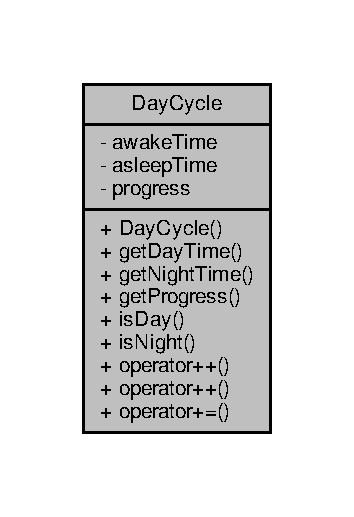
\includegraphics[width=170pt]{classDayCycle__coll__graph}
\end{center}
\end{figure}
\subsection*{Public Member Functions}
\begin{DoxyCompactItemize}
\item 
\hyperlink{classDayCycle_a9a2d185823b938e0ff6a74d21b5225a5_a9a2d185823b938e0ff6a74d21b5225a5}{Day\+Cycle} (unsigned int=0, unsigned int=0)
\item 
int \hyperlink{classDayCycle_a9bd40be57103509887314494419c7f1b_a9bd40be57103509887314494419c7f1b}{get\+Day\+Time} () const
\item 
int \hyperlink{classDayCycle_aeeb7012fe96467e4a179a195e8851d82_aeeb7012fe96467e4a179a195e8851d82}{get\+Night\+Time} () const
\item 
int \hyperlink{classDayCycle_aab4c411cdcb1b80daa5219a6aa339ebe_aab4c411cdcb1b80daa5219a6aa339ebe}{get\+Progress} () const
\item 
bool \hyperlink{classDayCycle_a143c56cd6f6bd7ff5a3b73e385ec771e_a143c56cd6f6bd7ff5a3b73e385ec771e}{is\+Day} () const
\item 
bool \hyperlink{classDayCycle_aac8bd32b0e81f5b30d2853abb5925d3e_aac8bd32b0e81f5b30d2853abb5925d3e}{is\+Night} () const
\item 
\hyperlink{classDayCycle}{Day\+Cycle} \& \hyperlink{classDayCycle_a44a7b511e82ac36f4937867a6ff0de99_a44a7b511e82ac36f4937867a6ff0de99}{operator++} ()
\item 
\hyperlink{classDayCycle}{Day\+Cycle} \hyperlink{classDayCycle_a50cc0f4f794586eeaf44dba56beb6880_a50cc0f4f794586eeaf44dba56beb6880}{operator++} (int)
\item 
\hyperlink{classDayCycle}{Day\+Cycle} \& \hyperlink{classDayCycle_ad4603ee10b8a03540cefaa39070a3c98_ad4603ee10b8a03540cefaa39070a3c98}{operator+=} (int)
\end{DoxyCompactItemize}
\subsection*{Private Attributes}
\begin{DoxyCompactItemize}
\item 
unsigned int \hyperlink{classDayCycle_ac53e82e6492f02405b3336bf9ac3c606_ac53e82e6492f02405b3336bf9ac3c606}{awake\+Time}
\item 
unsigned int \hyperlink{classDayCycle_af544568ce6c2e04a2f04a76331a9ce05_af544568ce6c2e04a2f04a76331a9ce05}{asleep\+Time}
\item 
unsigned int \hyperlink{classDayCycle_ac1a08b3deca37cf2f182406d956876f3_ac1a08b3deca37cf2f182406d956876f3}{progress}
\end{DoxyCompactItemize}


\subsection{Constructor \& Destructor Documentation}
\mbox{\Hypertarget{classDayCycle_a9a2d185823b938e0ff6a74d21b5225a5_a9a2d185823b938e0ff6a74d21b5225a5}\label{classDayCycle_a9a2d185823b938e0ff6a74d21b5225a5_a9a2d185823b938e0ff6a74d21b5225a5}} 
\index{Day\+Cycle@{Day\+Cycle}!Day\+Cycle@{Day\+Cycle}}
\index{Day\+Cycle@{Day\+Cycle}!Day\+Cycle@{Day\+Cycle}}
\subsubsection{\texorpdfstring{Day\+Cycle()}{DayCycle()}}
{\footnotesize\ttfamily Day\+Cycle\+::\+Day\+Cycle (\begin{DoxyParamCaption}\item[{unsigned int}]{day = {\ttfamily 0},  }\item[{unsigned int}]{night = {\ttfamily 0} }\end{DoxyParamCaption})}



\subsection{Member Function Documentation}
\mbox{\Hypertarget{classDayCycle_a9bd40be57103509887314494419c7f1b_a9bd40be57103509887314494419c7f1b}\label{classDayCycle_a9bd40be57103509887314494419c7f1b_a9bd40be57103509887314494419c7f1b}} 
\index{Day\+Cycle@{Day\+Cycle}!get\+Day\+Time@{get\+Day\+Time}}
\index{get\+Day\+Time@{get\+Day\+Time}!Day\+Cycle@{Day\+Cycle}}
\subsubsection{\texorpdfstring{get\+Day\+Time()}{getDayTime()}}
{\footnotesize\ttfamily int Day\+Cycle\+::get\+Day\+Time (\begin{DoxyParamCaption}{ }\end{DoxyParamCaption}) const}

\mbox{\Hypertarget{classDayCycle_aeeb7012fe96467e4a179a195e8851d82_aeeb7012fe96467e4a179a195e8851d82}\label{classDayCycle_aeeb7012fe96467e4a179a195e8851d82_aeeb7012fe96467e4a179a195e8851d82}} 
\index{Day\+Cycle@{Day\+Cycle}!get\+Night\+Time@{get\+Night\+Time}}
\index{get\+Night\+Time@{get\+Night\+Time}!Day\+Cycle@{Day\+Cycle}}
\subsubsection{\texorpdfstring{get\+Night\+Time()}{getNightTime()}}
{\footnotesize\ttfamily int Day\+Cycle\+::get\+Night\+Time (\begin{DoxyParamCaption}{ }\end{DoxyParamCaption}) const}

\mbox{\Hypertarget{classDayCycle_aab4c411cdcb1b80daa5219a6aa339ebe_aab4c411cdcb1b80daa5219a6aa339ebe}\label{classDayCycle_aab4c411cdcb1b80daa5219a6aa339ebe_aab4c411cdcb1b80daa5219a6aa339ebe}} 
\index{Day\+Cycle@{Day\+Cycle}!get\+Progress@{get\+Progress}}
\index{get\+Progress@{get\+Progress}!Day\+Cycle@{Day\+Cycle}}
\subsubsection{\texorpdfstring{get\+Progress()}{getProgress()}}
{\footnotesize\ttfamily int Day\+Cycle\+::get\+Progress (\begin{DoxyParamCaption}{ }\end{DoxyParamCaption}) const}

\mbox{\Hypertarget{classDayCycle_a143c56cd6f6bd7ff5a3b73e385ec771e_a143c56cd6f6bd7ff5a3b73e385ec771e}\label{classDayCycle_a143c56cd6f6bd7ff5a3b73e385ec771e_a143c56cd6f6bd7ff5a3b73e385ec771e}} 
\index{Day\+Cycle@{Day\+Cycle}!is\+Day@{is\+Day}}
\index{is\+Day@{is\+Day}!Day\+Cycle@{Day\+Cycle}}
\subsubsection{\texorpdfstring{is\+Day()}{isDay()}}
{\footnotesize\ttfamily bool Day\+Cycle\+::is\+Day (\begin{DoxyParamCaption}{ }\end{DoxyParamCaption}) const}

\mbox{\Hypertarget{classDayCycle_aac8bd32b0e81f5b30d2853abb5925d3e_aac8bd32b0e81f5b30d2853abb5925d3e}\label{classDayCycle_aac8bd32b0e81f5b30d2853abb5925d3e_aac8bd32b0e81f5b30d2853abb5925d3e}} 
\index{Day\+Cycle@{Day\+Cycle}!is\+Night@{is\+Night}}
\index{is\+Night@{is\+Night}!Day\+Cycle@{Day\+Cycle}}
\subsubsection{\texorpdfstring{is\+Night()}{isNight()}}
{\footnotesize\ttfamily bool Day\+Cycle\+::is\+Night (\begin{DoxyParamCaption}{ }\end{DoxyParamCaption}) const}

\mbox{\Hypertarget{classDayCycle_a44a7b511e82ac36f4937867a6ff0de99_a44a7b511e82ac36f4937867a6ff0de99}\label{classDayCycle_a44a7b511e82ac36f4937867a6ff0de99_a44a7b511e82ac36f4937867a6ff0de99}} 
\index{Day\+Cycle@{Day\+Cycle}!operator++@{operator++}}
\index{operator++@{operator++}!Day\+Cycle@{Day\+Cycle}}
\subsubsection{\texorpdfstring{operator++()}{operator++()}\hspace{0.1cm}{\footnotesize\ttfamily [1/2]}}
{\footnotesize\ttfamily \hyperlink{classDayCycle}{Day\+Cycle} \& Day\+Cycle\+::operator++ (\begin{DoxyParamCaption}{ }\end{DoxyParamCaption})}

\mbox{\Hypertarget{classDayCycle_a50cc0f4f794586eeaf44dba56beb6880_a50cc0f4f794586eeaf44dba56beb6880}\label{classDayCycle_a50cc0f4f794586eeaf44dba56beb6880_a50cc0f4f794586eeaf44dba56beb6880}} 
\index{Day\+Cycle@{Day\+Cycle}!operator++@{operator++}}
\index{operator++@{operator++}!Day\+Cycle@{Day\+Cycle}}
\subsubsection{\texorpdfstring{operator++()}{operator++()}\hspace{0.1cm}{\footnotesize\ttfamily [2/2]}}
{\footnotesize\ttfamily \hyperlink{classDayCycle}{Day\+Cycle} Day\+Cycle\+::operator++ (\begin{DoxyParamCaption}\item[{int}]{ }\end{DoxyParamCaption})}

\mbox{\Hypertarget{classDayCycle_ad4603ee10b8a03540cefaa39070a3c98_ad4603ee10b8a03540cefaa39070a3c98}\label{classDayCycle_ad4603ee10b8a03540cefaa39070a3c98_ad4603ee10b8a03540cefaa39070a3c98}} 
\index{Day\+Cycle@{Day\+Cycle}!operator+=@{operator+=}}
\index{operator+=@{operator+=}!Day\+Cycle@{Day\+Cycle}}
\subsubsection{\texorpdfstring{operator+=()}{operator+=()}}
{\footnotesize\ttfamily \hyperlink{classDayCycle}{Day\+Cycle} \& Day\+Cycle\+::operator+= (\begin{DoxyParamCaption}\item[{int}]{increment }\end{DoxyParamCaption})}



\subsection{Member Data Documentation}
\mbox{\Hypertarget{classDayCycle_af544568ce6c2e04a2f04a76331a9ce05_af544568ce6c2e04a2f04a76331a9ce05}\label{classDayCycle_af544568ce6c2e04a2f04a76331a9ce05_af544568ce6c2e04a2f04a76331a9ce05}} 
\index{Day\+Cycle@{Day\+Cycle}!asleep\+Time@{asleep\+Time}}
\index{asleep\+Time@{asleep\+Time}!Day\+Cycle@{Day\+Cycle}}
\subsubsection{\texorpdfstring{asleep\+Time}{asleepTime}}
{\footnotesize\ttfamily unsigned int Day\+Cycle\+::asleep\+Time\hspace{0.3cm}{\ttfamily [private]}}

\mbox{\Hypertarget{classDayCycle_ac53e82e6492f02405b3336bf9ac3c606_ac53e82e6492f02405b3336bf9ac3c606}\label{classDayCycle_ac53e82e6492f02405b3336bf9ac3c606_ac53e82e6492f02405b3336bf9ac3c606}} 
\index{Day\+Cycle@{Day\+Cycle}!awake\+Time@{awake\+Time}}
\index{awake\+Time@{awake\+Time}!Day\+Cycle@{Day\+Cycle}}
\subsubsection{\texorpdfstring{awake\+Time}{awakeTime}}
{\footnotesize\ttfamily unsigned int Day\+Cycle\+::awake\+Time\hspace{0.3cm}{\ttfamily [private]}}

\mbox{\Hypertarget{classDayCycle_ac1a08b3deca37cf2f182406d956876f3_ac1a08b3deca37cf2f182406d956876f3}\label{classDayCycle_ac1a08b3deca37cf2f182406d956876f3_ac1a08b3deca37cf2f182406d956876f3}} 
\index{Day\+Cycle@{Day\+Cycle}!progress@{progress}}
\index{progress@{progress}!Day\+Cycle@{Day\+Cycle}}
\subsubsection{\texorpdfstring{progress}{progress}}
{\footnotesize\ttfamily unsigned int Day\+Cycle\+::progress\hspace{0.3cm}{\ttfamily [private]}}



The documentation for this class was generated from the following files\+:\begin{DoxyCompactItemize}
\item 
include/\hyperlink{daycycle_8hpp}{daycycle.\+hpp}\item 
src/\hyperlink{daycycle_8cpp}{daycycle.\+cpp}\end{DoxyCompactItemize}

\hypertarget{classDeepPtr}{}\section{Deep\+Ptr$<$ T $>$ Class Template Reference}
\label{classDeepPtr}\index{Deep\+Ptr$<$ T $>$@{Deep\+Ptr$<$ T $>$}}


{\ttfamily \#include $<$deepptr.\+hpp$>$}



Inheritance diagram for Deep\+Ptr$<$ T $>$\+:\nopagebreak
\begin{figure}[H]
\begin{center}
\leavevmode
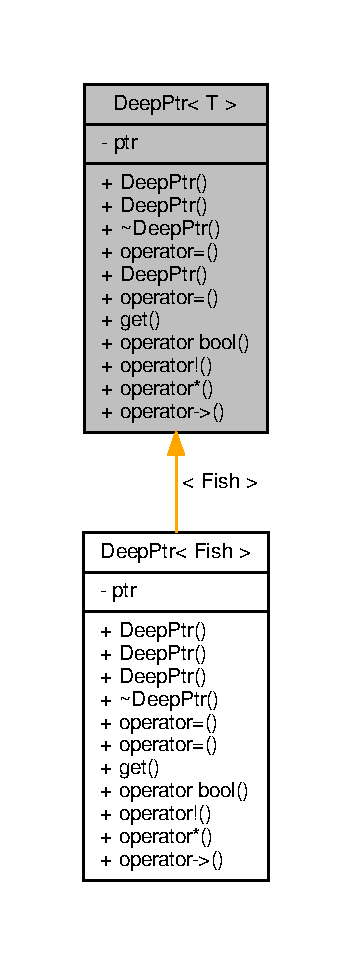
\includegraphics[width=169pt]{classDeepPtr__inherit__graph}
\end{center}
\end{figure}


Collaboration diagram for Deep\+Ptr$<$ T $>$\+:\nopagebreak
\begin{figure}[H]
\begin{center}
\leavevmode
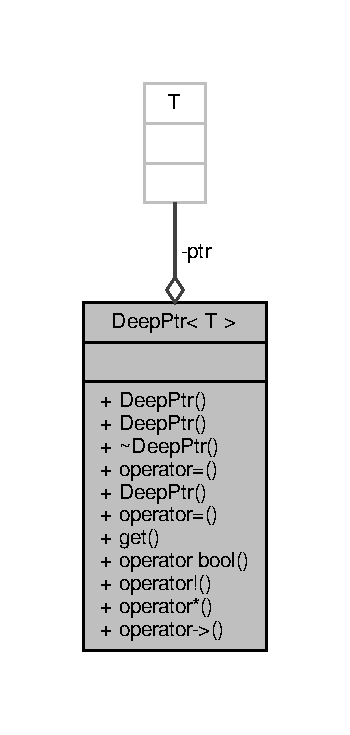
\includegraphics[width=168pt]{classDeepPtr__coll__graph}
\end{center}
\end{figure}
\subsection*{Public Member Functions}
\begin{DoxyCompactItemize}
\item 
\hyperlink{classDeepPtr_a85b1300bf23784588d48939280fad384_a85b1300bf23784588d48939280fad384}{Deep\+Ptr} (T $\ast$=nullptr)
\item 
\hyperlink{classDeepPtr_adfa6604344126aad1293c5d8d1132dad_adfa6604344126aad1293c5d8d1132dad}{Deep\+Ptr} (const \hyperlink{classDeepPtr}{Deep\+Ptr} \&d)
\item 
\hyperlink{classDeepPtr_ae9e23e5eb0c9d6f4a3621d2a2d9ed1c9_ae9e23e5eb0c9d6f4a3621d2a2d9ed1c9}{$\sim$\+Deep\+Ptr} ()
\item 
\hyperlink{classDeepPtr}{Deep\+Ptr} \& \hyperlink{classDeepPtr_a52350f0618e9385f3a3d3fd97ec5ea0b_a52350f0618e9385f3a3d3fd97ec5ea0b}{operator=} (const \hyperlink{classDeepPtr}{Deep\+Ptr} \&d)
\item 
\hyperlink{classDeepPtr_ae620731998d59ab7e60be48b081845c8_ae620731998d59ab7e60be48b081845c8}{Deep\+Ptr} (\hyperlink{classDeepPtr}{Deep\+Ptr} \&\&d)
\item 
\hyperlink{classDeepPtr}{Deep\+Ptr} \& \hyperlink{classDeepPtr_a00ff7a47f4cab7fa20de5fd5b6546756_a00ff7a47f4cab7fa20de5fd5b6546756}{operator=} (\hyperlink{classDeepPtr}{Deep\+Ptr} \&\&d)
\item 
T $\ast$ \hyperlink{classDeepPtr_a516165073b1c5f26e25af5cc479e55e9_a516165073b1c5f26e25af5cc479e55e9}{get} () const
\item 
\hyperlink{classDeepPtr_a2a14ae8e401d478df8217d4ced9d68e5_a2a14ae8e401d478df8217d4ced9d68e5}{operator bool} () const
\item 
bool \hyperlink{classDeepPtr_ab56cff47e67dd4b60b7680ec47f63cfc_ab56cff47e67dd4b60b7680ec47f63cfc}{operator!} () const
\item 
T \& \hyperlink{classDeepPtr_a3e338b1c727ea5e291ebe65588c37ec3_a3e338b1c727ea5e291ebe65588c37ec3}{operator$\ast$} () const
\item 
T $\ast$ \hyperlink{classDeepPtr_ac9c2935e0a0ec88bf52a6695ace6d7bb_ac9c2935e0a0ec88bf52a6695ace6d7bb}{operator-\/$>$} () const
\end{DoxyCompactItemize}
\subsection*{Private Attributes}
\begin{DoxyCompactItemize}
\item 
T $\ast$ \hyperlink{classDeepPtr_aa738303c3bb2c634b6edfee93bdf2a07_aa738303c3bb2c634b6edfee93bdf2a07}{ptr}
\end{DoxyCompactItemize}


\subsection{Constructor \& Destructor Documentation}
\mbox{\Hypertarget{classDeepPtr_a85b1300bf23784588d48939280fad384_a85b1300bf23784588d48939280fad384}\label{classDeepPtr_a85b1300bf23784588d48939280fad384_a85b1300bf23784588d48939280fad384}} 
\index{Deep\+Ptr@{Deep\+Ptr}!Deep\+Ptr@{Deep\+Ptr}}
\index{Deep\+Ptr@{Deep\+Ptr}!Deep\+Ptr@{Deep\+Ptr}}
\subsubsection{\texorpdfstring{Deep\+Ptr()}{DeepPtr()}\hspace{0.1cm}{\footnotesize\ttfamily [1/3]}}
{\footnotesize\ttfamily template$<$class T$>$ \\
\hyperlink{classDeepPtr}{Deep\+Ptr}$<$ T $>$\+::\hyperlink{classDeepPtr}{Deep\+Ptr} (\begin{DoxyParamCaption}\item[{T $\ast$}]{p = {\ttfamily nullptr} }\end{DoxyParamCaption})}

\mbox{\Hypertarget{classDeepPtr_adfa6604344126aad1293c5d8d1132dad_adfa6604344126aad1293c5d8d1132dad}\label{classDeepPtr_adfa6604344126aad1293c5d8d1132dad_adfa6604344126aad1293c5d8d1132dad}} 
\index{Deep\+Ptr@{Deep\+Ptr}!Deep\+Ptr@{Deep\+Ptr}}
\index{Deep\+Ptr@{Deep\+Ptr}!Deep\+Ptr@{Deep\+Ptr}}
\subsubsection{\texorpdfstring{Deep\+Ptr()}{DeepPtr()}\hspace{0.1cm}{\footnotesize\ttfamily [2/3]}}
{\footnotesize\ttfamily template$<$class T$>$ \\
\hyperlink{classDeepPtr}{Deep\+Ptr}$<$ T $>$\+::\hyperlink{classDeepPtr}{Deep\+Ptr} (\begin{DoxyParamCaption}\item[{const \hyperlink{classDeepPtr}{Deep\+Ptr}$<$ T $>$ \&}]{d }\end{DoxyParamCaption})}

\mbox{\Hypertarget{classDeepPtr_ae9e23e5eb0c9d6f4a3621d2a2d9ed1c9_ae9e23e5eb0c9d6f4a3621d2a2d9ed1c9}\label{classDeepPtr_ae9e23e5eb0c9d6f4a3621d2a2d9ed1c9_ae9e23e5eb0c9d6f4a3621d2a2d9ed1c9}} 
\index{Deep\+Ptr@{Deep\+Ptr}!````~Deep\+Ptr@{$\sim$\+Deep\+Ptr}}
\index{````~Deep\+Ptr@{$\sim$\+Deep\+Ptr}!Deep\+Ptr@{Deep\+Ptr}}
\subsubsection{\texorpdfstring{$\sim$\+Deep\+Ptr()}{~DeepPtr()}}
{\footnotesize\ttfamily template$<$class T $>$ \\
\hyperlink{classDeepPtr}{Deep\+Ptr}$<$ T $>$\+::$\sim$\hyperlink{classDeepPtr}{Deep\+Ptr} (\begin{DoxyParamCaption}{ }\end{DoxyParamCaption})}

\mbox{\Hypertarget{classDeepPtr_ae620731998d59ab7e60be48b081845c8_ae620731998d59ab7e60be48b081845c8}\label{classDeepPtr_ae620731998d59ab7e60be48b081845c8_ae620731998d59ab7e60be48b081845c8}} 
\index{Deep\+Ptr@{Deep\+Ptr}!Deep\+Ptr@{Deep\+Ptr}}
\index{Deep\+Ptr@{Deep\+Ptr}!Deep\+Ptr@{Deep\+Ptr}}
\subsubsection{\texorpdfstring{Deep\+Ptr()}{DeepPtr()}\hspace{0.1cm}{\footnotesize\ttfamily [3/3]}}
{\footnotesize\ttfamily template$<$class T$>$ \\
\hyperlink{classDeepPtr}{Deep\+Ptr}$<$ T $>$\+::\hyperlink{classDeepPtr}{Deep\+Ptr} (\begin{DoxyParamCaption}\item[{\hyperlink{classDeepPtr}{Deep\+Ptr}$<$ T $>$ \&\&}]{d }\end{DoxyParamCaption})}



\subsection{Member Function Documentation}
\mbox{\Hypertarget{classDeepPtr_a516165073b1c5f26e25af5cc479e55e9_a516165073b1c5f26e25af5cc479e55e9}\label{classDeepPtr_a516165073b1c5f26e25af5cc479e55e9_a516165073b1c5f26e25af5cc479e55e9}} 
\index{Deep\+Ptr@{Deep\+Ptr}!get@{get}}
\index{get@{get}!Deep\+Ptr@{Deep\+Ptr}}
\subsubsection{\texorpdfstring{get()}{get()}}
{\footnotesize\ttfamily template$<$class T $>$ \\
T $\ast$ \hyperlink{classDeepPtr}{Deep\+Ptr}$<$ T $>$\+::get (\begin{DoxyParamCaption}{ }\end{DoxyParamCaption}) const}

\mbox{\Hypertarget{classDeepPtr_a2a14ae8e401d478df8217d4ced9d68e5_a2a14ae8e401d478df8217d4ced9d68e5}\label{classDeepPtr_a2a14ae8e401d478df8217d4ced9d68e5_a2a14ae8e401d478df8217d4ced9d68e5}} 
\index{Deep\+Ptr@{Deep\+Ptr}!operator bool@{operator bool}}
\index{operator bool@{operator bool}!Deep\+Ptr@{Deep\+Ptr}}
\subsubsection{\texorpdfstring{operator bool()}{operator bool()}}
{\footnotesize\ttfamily template$<$class T $>$ \\
\hyperlink{classDeepPtr}{Deep\+Ptr}$<$ T $>$\+::operator bool (\begin{DoxyParamCaption}{ }\end{DoxyParamCaption}) const}

\mbox{\Hypertarget{classDeepPtr_ab56cff47e67dd4b60b7680ec47f63cfc_ab56cff47e67dd4b60b7680ec47f63cfc}\label{classDeepPtr_ab56cff47e67dd4b60b7680ec47f63cfc_ab56cff47e67dd4b60b7680ec47f63cfc}} 
\index{Deep\+Ptr@{Deep\+Ptr}!operator"!@{operator"!}}
\index{operator"!@{operator"!}!Deep\+Ptr@{Deep\+Ptr}}
\subsubsection{\texorpdfstring{operator"!()}{operator!()}}
{\footnotesize\ttfamily template$<$class T $>$ \\
bool \hyperlink{classDeepPtr}{Deep\+Ptr}$<$ T $>$\+::operator! (\begin{DoxyParamCaption}{ }\end{DoxyParamCaption}) const}

\mbox{\Hypertarget{classDeepPtr_a3e338b1c727ea5e291ebe65588c37ec3_a3e338b1c727ea5e291ebe65588c37ec3}\label{classDeepPtr_a3e338b1c727ea5e291ebe65588c37ec3_a3e338b1c727ea5e291ebe65588c37ec3}} 
\index{Deep\+Ptr@{Deep\+Ptr}!operator$\ast$@{operator$\ast$}}
\index{operator$\ast$@{operator$\ast$}!Deep\+Ptr@{Deep\+Ptr}}
\subsubsection{\texorpdfstring{operator$\ast$()}{operator*()}}
{\footnotesize\ttfamily template$<$class T $>$ \\
T \& \hyperlink{classDeepPtr}{Deep\+Ptr}$<$ T $>$\+::operator$\ast$ (\begin{DoxyParamCaption}{ }\end{DoxyParamCaption}) const}

\mbox{\Hypertarget{classDeepPtr_ac9c2935e0a0ec88bf52a6695ace6d7bb_ac9c2935e0a0ec88bf52a6695ace6d7bb}\label{classDeepPtr_ac9c2935e0a0ec88bf52a6695ace6d7bb_ac9c2935e0a0ec88bf52a6695ace6d7bb}} 
\index{Deep\+Ptr@{Deep\+Ptr}!operator-\/$>$@{operator-\/$>$}}
\index{operator-\/$>$@{operator-\/$>$}!Deep\+Ptr@{Deep\+Ptr}}
\subsubsection{\texorpdfstring{operator-\/$>$()}{operator->()}}
{\footnotesize\ttfamily template$<$class T $>$ \\
T $\ast$ \hyperlink{classDeepPtr}{Deep\+Ptr}$<$ T $>$\+::operator-\/$>$ (\begin{DoxyParamCaption}{ }\end{DoxyParamCaption}) const}

\mbox{\Hypertarget{classDeepPtr_a52350f0618e9385f3a3d3fd97ec5ea0b_a52350f0618e9385f3a3d3fd97ec5ea0b}\label{classDeepPtr_a52350f0618e9385f3a3d3fd97ec5ea0b_a52350f0618e9385f3a3d3fd97ec5ea0b}} 
\index{Deep\+Ptr@{Deep\+Ptr}!operator=@{operator=}}
\index{operator=@{operator=}!Deep\+Ptr@{Deep\+Ptr}}
\subsubsection{\texorpdfstring{operator=()}{operator=()}\hspace{0.1cm}{\footnotesize\ttfamily [1/2]}}
{\footnotesize\ttfamily template$<$class T $>$ \\
\hyperlink{classDeepPtr}{Deep\+Ptr}$<$ T $>$ \& \hyperlink{classDeepPtr}{Deep\+Ptr}$<$ T $>$\+::operator= (\begin{DoxyParamCaption}\item[{const \hyperlink{classDeepPtr}{Deep\+Ptr}$<$ T $>$ \&}]{d }\end{DoxyParamCaption})}

\mbox{\Hypertarget{classDeepPtr_a00ff7a47f4cab7fa20de5fd5b6546756_a00ff7a47f4cab7fa20de5fd5b6546756}\label{classDeepPtr_a00ff7a47f4cab7fa20de5fd5b6546756_a00ff7a47f4cab7fa20de5fd5b6546756}} 
\index{Deep\+Ptr@{Deep\+Ptr}!operator=@{operator=}}
\index{operator=@{operator=}!Deep\+Ptr@{Deep\+Ptr}}
\subsubsection{\texorpdfstring{operator=()}{operator=()}\hspace{0.1cm}{\footnotesize\ttfamily [2/2]}}
{\footnotesize\ttfamily template$<$class T $>$ \\
\hyperlink{classDeepPtr}{Deep\+Ptr}$<$ T $>$ \& \hyperlink{classDeepPtr}{Deep\+Ptr}$<$ T $>$\+::operator= (\begin{DoxyParamCaption}\item[{\hyperlink{classDeepPtr}{Deep\+Ptr}$<$ T $>$ \&\&}]{d }\end{DoxyParamCaption})}



\subsection{Member Data Documentation}
\mbox{\Hypertarget{classDeepPtr_aa738303c3bb2c634b6edfee93bdf2a07_aa738303c3bb2c634b6edfee93bdf2a07}\label{classDeepPtr_aa738303c3bb2c634b6edfee93bdf2a07_aa738303c3bb2c634b6edfee93bdf2a07}} 
\index{Deep\+Ptr@{Deep\+Ptr}!ptr@{ptr}}
\index{ptr@{ptr}!Deep\+Ptr@{Deep\+Ptr}}
\subsubsection{\texorpdfstring{ptr}{ptr}}
{\footnotesize\ttfamily template$<$class T$>$ \\
T$\ast$ \hyperlink{classDeepPtr}{Deep\+Ptr}$<$ T $>$\+::ptr\hspace{0.3cm}{\ttfamily [private]}}



The documentation for this class was generated from the following file\+:\begin{DoxyCompactItemize}
\item 
include/\hyperlink{deepptr_8hpp}{deepptr.\+hpp}\end{DoxyCompactItemize}

\hypertarget{classFish}{}\section{Fish Class Reference}
\label{classFish}\index{Fish@{Fish}}


{\ttfamily \#include $<$fish.\+hpp$>$}



Inheritance diagram for Fish\+:\nopagebreak
\begin{figure}[H]
\begin{center}
\leavevmode
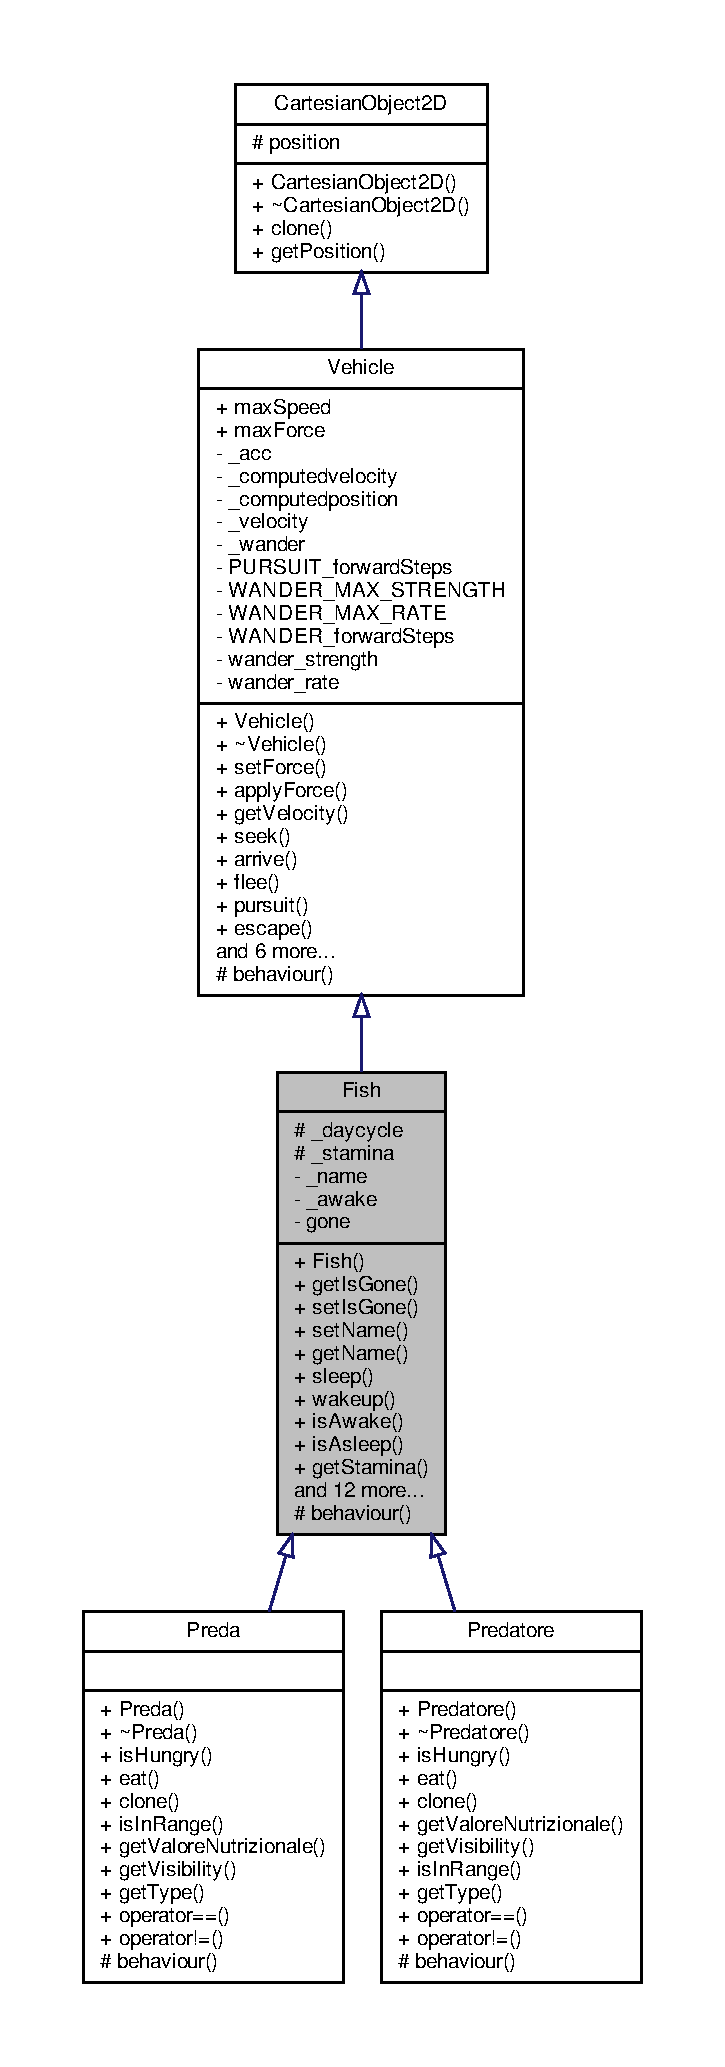
\includegraphics[height=550pt]{classFish__inherit__graph}
\end{center}
\end{figure}


Collaboration diagram for Fish\+:\nopagebreak
\begin{figure}[H]
\begin{center}
\leavevmode
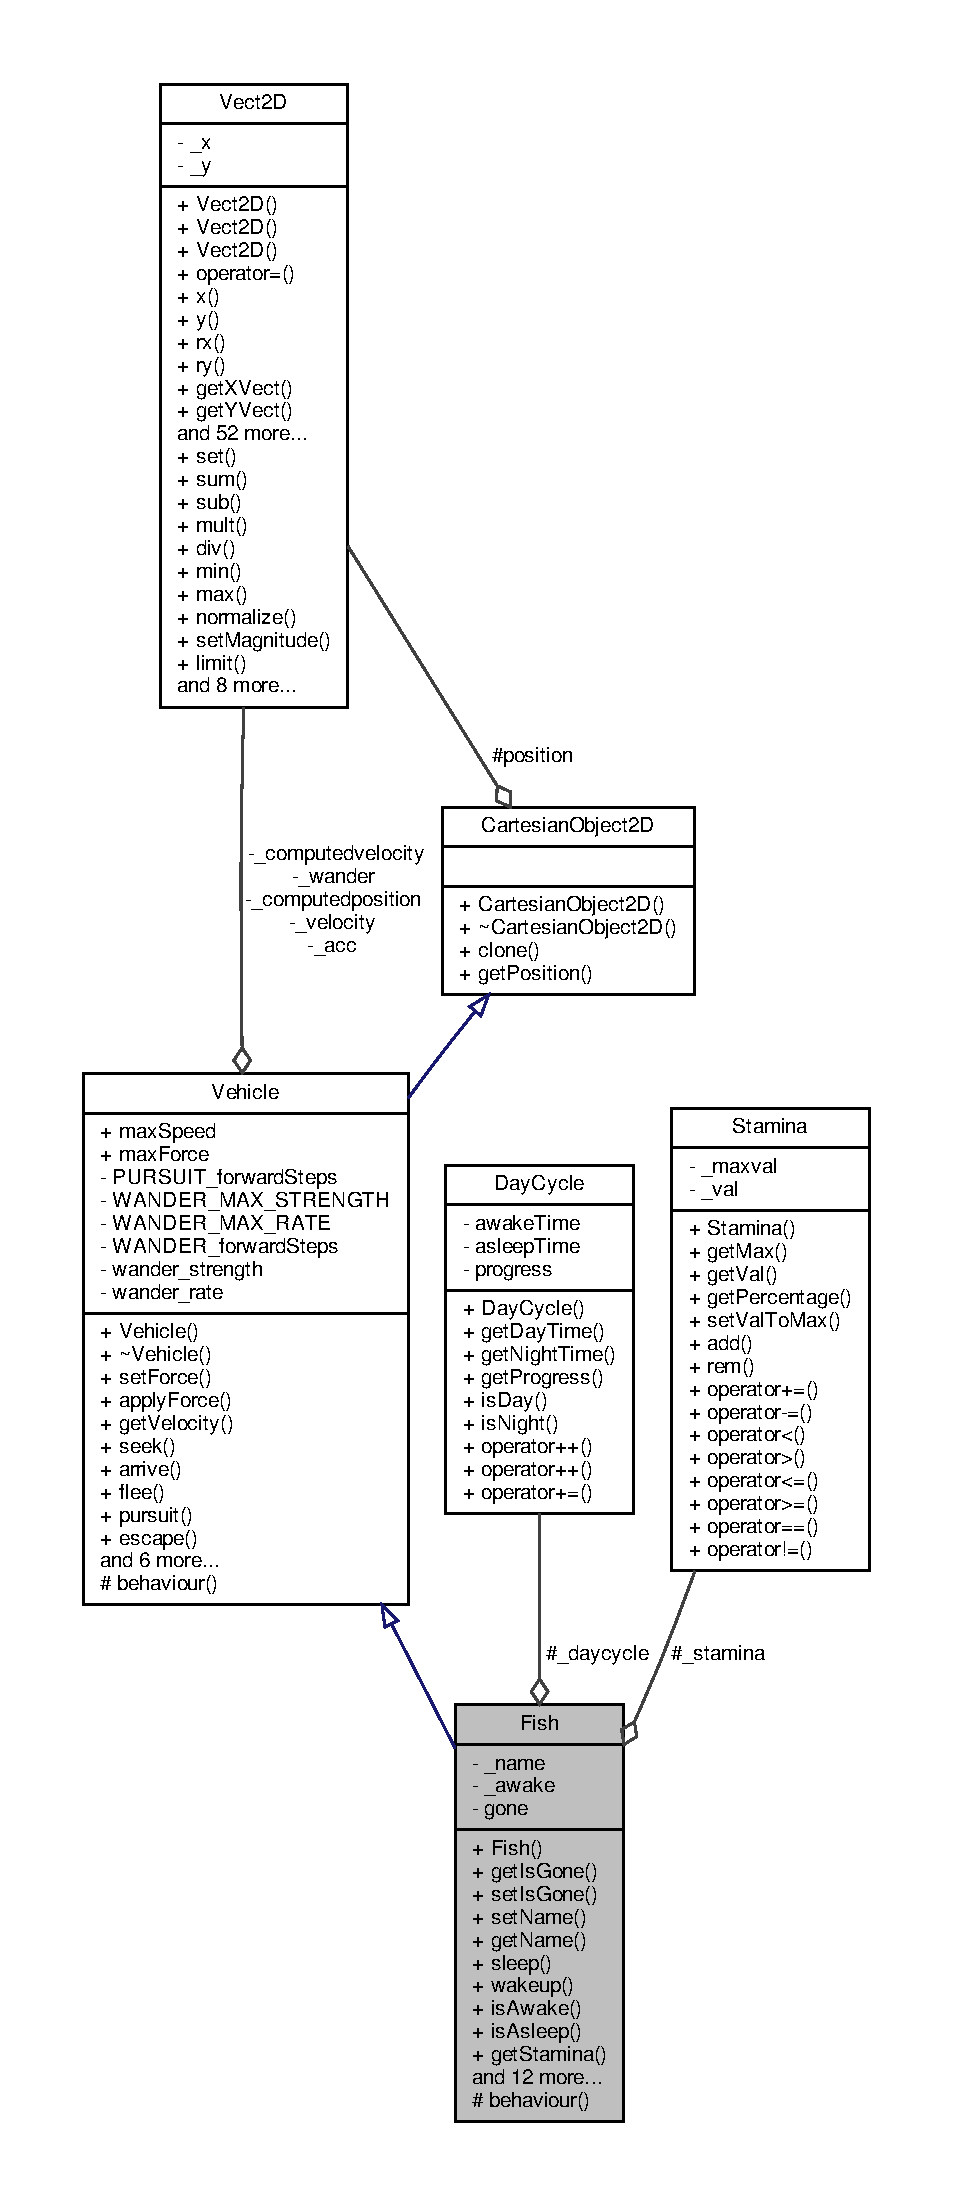
\includegraphics[height=550pt]{classFish__coll__graph}
\end{center}
\end{figure}
\subsection*{Public Member Functions}
\begin{DoxyCompactItemize}
\item 
\hyperlink{classFish_a7f97c2f2fea7930e5c82b8e7edd382ac_a7f97c2f2fea7930e5c82b8e7edd382ac}{Fish} (const std\+::string \&, unsigned int, unsigned int, double)
\item 
bool \hyperlink{classFish_a64e050916c0094ac377b8ec0d86a000b_a64e050916c0094ac377b8ec0d86a000b}{get\+Is\+Gone} () const
\item 
void \hyperlink{classFish_ad7d3a39831fa4a170a63dde98474b728_ad7d3a39831fa4a170a63dde98474b728}{set\+Is\+Gone} ()
\item 
void \hyperlink{classFish_a27a489adca6d1dc91b011ee97f36ae75_a27a489adca6d1dc91b011ee97f36ae75}{set\+Name} (const std\+::string \&)
\item 
const std\+::string \& \hyperlink{classFish_a96583314997aab0826f1c595f7d58938_a96583314997aab0826f1c595f7d58938}{get\+Name} () const
\item 
void \hyperlink{classFish_acac2f4f6c31adfb0c8f4eb78853445bb_acac2f4f6c31adfb0c8f4eb78853445bb}{sleep} ()
\item 
void \hyperlink{classFish_a8160593a43c6ce5263c6280e0cf0a7be_a8160593a43c6ce5263c6280e0cf0a7be}{wakeup} ()
\item 
bool \hyperlink{classFish_aea2a66c3cd46d3a672c82ca9e537b9ec_aea2a66c3cd46d3a672c82ca9e537b9ec}{is\+Awake} () const
\item 
bool \hyperlink{classFish_a4772391eb9a92dca61b810b40705709b_a4772391eb9a92dca61b810b40705709b}{is\+Asleep} () const
\item 
const \hyperlink{classStamina}{Stamina} \& \hyperlink{classFish_a8637a567ecb17376bed45783d5ddb53d_a8637a567ecb17376bed45783d5ddb53d}{get\+Stamina} () const
\item 
virtual \hyperlink{classFish_a23885c7956e22f0181360098cfe16659_a23885c7956e22f0181360098cfe16659}{$\sim$\+Fish} ()
\item 
virtual bool \hyperlink{classFish_a5fa8678bf28b723cfd2e225c217bb523_a5fa8678bf28b723cfd2e225c217bb523}{is\+Hungry} () const =0
\item 
virtual bool \hyperlink{classFish_a9a94edb09498e8d0d2381c2cc3e2e9dc_a9a94edb09498e8d0d2381c2cc3e2e9dc}{can\+Sleep} () const
\item 
virtual bool \hyperlink{classFish_a033298bf0dc885b82dbd195fc4997643_a033298bf0dc885b82dbd195fc4997643}{can\+Wakeup} () const
\item 
virtual void \hyperlink{classFish_ae551e094ddda73e896de484dcb460412_ae551e094ddda73e896de484dcb460412}{eat} (\hyperlink{classFish}{Fish} \&)=0
\item 
virtual std\+::string \hyperlink{classFish_adb00fb6bac2fad27660107c12d1a7fa2_adb00fb6bac2fad27660107c12d1a7fa2}{get\+Type} () const =0
\item 
virtual int \hyperlink{classFish_a97dd71f31af1e36a630944c5c5b8ff33_a97dd71f31af1e36a630944c5c5b8ff33}{get\+Valore\+Nutrizionale} () const =0
\item 
virtual double \hyperlink{classFish_a6c20ea483d1f6237ebf01aee3f2b6e88_a6c20ea483d1f6237ebf01aee3f2b6e88}{get\+Visibility} () const =0
\item 
virtual bool \hyperlink{classFish_a3abf96fe9cda276a4b3827464e2b0519_a3abf96fe9cda276a4b3827464e2b0519}{operator==} (const \hyperlink{classFish}{Fish} \&) const =0
\item 
virtual bool \hyperlink{classFish_aa739aa5c06ff6054b051047bccd3bf6f_aa739aa5c06ff6054b051047bccd3bf6f}{operator!=} (const \hyperlink{classFish}{Fish} \&) const =0
\item 
virtual \hyperlink{classFish}{Fish} $\ast$ \hyperlink{classFish_a6732945f7373a28b1723e55de8a65e13_a6732945f7373a28b1723e55de8a65e13}{clone} () const override=0
\item 
virtual bool \hyperlink{classFish_a65e3b0bf5b211be6c4048aa5939331e1_a65e3b0bf5b211be6c4048aa5939331e1}{is\+In\+Range} (const \hyperlink{classVect2D}{Vect2D} \&) const =0
\item 
void \hyperlink{classVehicle_a03e22c522e6f526f95428c81d0762833_a03e22c522e6f526f95428c81d0762833}{set\+Force} (const \hyperlink{classVect2D}{Vect2D} \&)
\item 
void \hyperlink{classVehicle_a82fbbd5aafc1ba89c3daa4da09989bbe_a82fbbd5aafc1ba89c3daa4da09989bbe}{apply\+Force} (const \hyperlink{classVect2D}{Vect2D} \&, const double \&=1)
\item 
const \hyperlink{classVect2D}{Vect2D} \& \hyperlink{classVehicle_a87b8266cb3495e8444233a0724e1bf07_a87b8266cb3495e8444233a0724e1bf07}{get\+Velocity} () const
\item 
\hyperlink{classVect2D}{Vect2D} \hyperlink{classVehicle_a86c0b5ddcf64443bc090657cd29832bf_a86c0b5ddcf64443bc090657cd29832bf}{seek} (const \hyperlink{classVect2D}{Vect2D} \&) const
\item 
\hyperlink{classVect2D}{Vect2D} \hyperlink{classVehicle_a55f8bb6cfbdd97219c2cea6cf3ad3826_a55f8bb6cfbdd97219c2cea6cf3ad3826}{arrive} (const \hyperlink{classVect2D}{Vect2D} \&) const
\item 
\hyperlink{classVect2D}{Vect2D} \hyperlink{classVehicle_ac7dbbb2942b8d642b2ab071def1c2fdb_ac7dbbb2942b8d642b2ab071def1c2fdb}{flee} (const \hyperlink{classVect2D}{Vect2D} \&) const
\item 
\hyperlink{classVect2D}{Vect2D} \hyperlink{classVehicle_a9dd4f4a06b4abd3324d317c27bb867d2_a9dd4f4a06b4abd3324d317c27bb867d2}{pursuit} (const \hyperlink{classVehicle}{Vehicle} \&) const
\item 
\hyperlink{classVect2D}{Vect2D} \hyperlink{classVehicle_ae5fbf395cbebf51498cbe8b2baaddc16_ae5fbf395cbebf51498cbe8b2baaddc16}{escape} (const \hyperlink{classVehicle}{Vehicle} \&) const
\item 
\hyperlink{classVect2D}{Vect2D} \hyperlink{classVehicle_af9da94116706c94e5f26df42c258dc6e_af9da94116706c94e5f26df42c258dc6e}{wander} ()
\item 
\hyperlink{classVect2D}{Vect2D} \hyperlink{classVehicle_a9a1cb1e5dab4a474fbe0c1c49482d0ee_a9a1cb1e5dab4a474fbe0c1c49482d0ee}{stop} () const
\item 
\hyperlink{classVect2D}{Vect2D} \hyperlink{classVehicle_a6149abf3e3f67df45d950562034d0fae_a6149abf3e3f67df45d950562034d0fae}{stay\+Within\+Borders} (const \hyperlink{classVect2D}{Vect2D} \&, const unsigned int distance) const
\item 
virtual void \hyperlink{classVehicle_aa4ffd7e5fd11297950347de4e8b5ec93_aa4ffd7e5fd11297950347de4e8b5ec93}{advance} (\hyperlink{classAquarius}{Aquarius} $\ast$a, int phase) final
\item 
\hyperlink{classVect2D}{Vect2D} \hyperlink{classCartesianObject2D_aa3a6b63777852ab9eb9408ed2536abe2_aa3a6b63777852ab9eb9408ed2536abe2}{get\+Position} () const
\end{DoxyCompactItemize}
\subsection*{Static Public Attributes}
\begin{DoxyCompactItemize}
\item 
static const double \hyperlink{classVehicle_aab47c62e89baa5b7e52c2292451fbcb6_aab47c62e89baa5b7e52c2292451fbcb6}{max\+Speed} = 5
\item 
static const double \hyperlink{classVehicle_a95c56790e3dc52ab0fa54c279920be54_a95c56790e3dc52ab0fa54c279920be54}{max\+Force} = .\+15
\end{DoxyCompactItemize}
\subsection*{Protected Member Functions}
\begin{DoxyCompactItemize}
\item 
virtual void \hyperlink{classFish_abffd423bc7a7730aafa80ec9c0cec9a0_abffd423bc7a7730aafa80ec9c0cec9a0}{behaviour} (\hyperlink{classAquarius}{Aquarius} $\ast$) override
\end{DoxyCompactItemize}
\subsection*{Protected Attributes}
\begin{DoxyCompactItemize}
\item 
\hyperlink{classDayCycle}{Day\+Cycle} \hyperlink{classFish_a4b8a32e2a5165ddd1f8af27f4346b3eb_a4b8a32e2a5165ddd1f8af27f4346b3eb}{\+\_\+daycycle}
\item 
\hyperlink{classStamina}{Stamina} \hyperlink{classFish_a4948331d0f556344bda8314828eec8dd_a4948331d0f556344bda8314828eec8dd}{\+\_\+stamina}
\item 
\hyperlink{classVect2D}{Vect2D} \hyperlink{classCartesianObject2D_ae02ec6ed11f9bfc0c748da033d6a32f9_ae02ec6ed11f9bfc0c748da033d6a32f9}{position}
\end{DoxyCompactItemize}
\subsection*{Private Attributes}
\begin{DoxyCompactItemize}
\item 
std\+::string \hyperlink{classFish_a0fff903c775250b77cb079ec291863a4_a0fff903c775250b77cb079ec291863a4}{\+\_\+name}
\item 
bool \hyperlink{classFish_a9298b505c56bb0c5480a3eff0cb8542b_a9298b505c56bb0c5480a3eff0cb8542b}{\+\_\+awake}
\item 
bool \hyperlink{classFish_a7daccde048dc63b7f8c9e6be0af56fa5_a7daccde048dc63b7f8c9e6be0af56fa5}{gone}
\end{DoxyCompactItemize}


\subsection{Constructor \& Destructor Documentation}
\mbox{\Hypertarget{classFish_a7f97c2f2fea7930e5c82b8e7edd382ac_a7f97c2f2fea7930e5c82b8e7edd382ac}\label{classFish_a7f97c2f2fea7930e5c82b8e7edd382ac_a7f97c2f2fea7930e5c82b8e7edd382ac}} 
\index{Fish@{Fish}!Fish@{Fish}}
\index{Fish@{Fish}!Fish@{Fish}}
\subsubsection{\texorpdfstring{Fish()}{Fish()}}
{\footnotesize\ttfamily Fish\+::\+Fish (\begin{DoxyParamCaption}\item[{const std\+::string \&}]{name,  }\item[{unsigned int}]{a,  }\item[{unsigned int}]{s,  }\item[{double}]{stam }\end{DoxyParamCaption})}

\mbox{\Hypertarget{classFish_a23885c7956e22f0181360098cfe16659_a23885c7956e22f0181360098cfe16659}\label{classFish_a23885c7956e22f0181360098cfe16659_a23885c7956e22f0181360098cfe16659}} 
\index{Fish@{Fish}!````~Fish@{$\sim$\+Fish}}
\index{````~Fish@{$\sim$\+Fish}!Fish@{Fish}}
\subsubsection{\texorpdfstring{$\sim$\+Fish()}{~Fish()}}
{\footnotesize\ttfamily Fish\+::$\sim$\+Fish (\begin{DoxyParamCaption}{ }\end{DoxyParamCaption})\hspace{0.3cm}{\ttfamily [virtual]}}



\subsection{Member Function Documentation}
\mbox{\Hypertarget{classVehicle_aa4ffd7e5fd11297950347de4e8b5ec93_aa4ffd7e5fd11297950347de4e8b5ec93}\label{classVehicle_aa4ffd7e5fd11297950347de4e8b5ec93_aa4ffd7e5fd11297950347de4e8b5ec93}} 
\index{Fish@{Fish}!advance@{advance}}
\index{advance@{advance}!Fish@{Fish}}
\subsubsection{\texorpdfstring{advance()}{advance()}}
{\footnotesize\ttfamily void Vehicle\+::advance (\begin{DoxyParamCaption}\item[{\hyperlink{classAquarius}{Aquarius} $\ast$}]{a,  }\item[{int}]{phase }\end{DoxyParamCaption})\hspace{0.3cm}{\ttfamily [final]}, {\ttfamily [virtual]}, {\ttfamily [inherited]}}

\mbox{\Hypertarget{classVehicle_a82fbbd5aafc1ba89c3daa4da09989bbe_a82fbbd5aafc1ba89c3daa4da09989bbe}\label{classVehicle_a82fbbd5aafc1ba89c3daa4da09989bbe_a82fbbd5aafc1ba89c3daa4da09989bbe}} 
\index{Fish@{Fish}!apply\+Force@{apply\+Force}}
\index{apply\+Force@{apply\+Force}!Fish@{Fish}}
\subsubsection{\texorpdfstring{apply\+Force()}{applyForce()}}
{\footnotesize\ttfamily void Vehicle\+::apply\+Force (\begin{DoxyParamCaption}\item[{const \hyperlink{classVect2D}{Vect2D} \&}]{acc,  }\item[{const double \&}]{weight = {\ttfamily 1} }\end{DoxyParamCaption})\hspace{0.3cm}{\ttfamily [inherited]}}

Add the force of acceleration, to the already calculated one 
\begin{DoxyParams}{Parameters}
{\em acc} & \\
\hline
{\em weight} & \\
\hline
\end{DoxyParams}
\mbox{\Hypertarget{classVehicle_a55f8bb6cfbdd97219c2cea6cf3ad3826_a55f8bb6cfbdd97219c2cea6cf3ad3826}\label{classVehicle_a55f8bb6cfbdd97219c2cea6cf3ad3826_a55f8bb6cfbdd97219c2cea6cf3ad3826}} 
\index{Fish@{Fish}!arrive@{arrive}}
\index{arrive@{arrive}!Fish@{Fish}}
\subsubsection{\texorpdfstring{arrive()}{arrive()}}
{\footnotesize\ttfamily \hyperlink{classVect2D}{Vect2D} Vehicle\+::arrive (\begin{DoxyParamCaption}\item[{const \hyperlink{classVect2D}{Vect2D} \&}]{target }\end{DoxyParamCaption}) const\hspace{0.3cm}{\ttfamily [inherited]}}

\mbox{\Hypertarget{classFish_abffd423bc7a7730aafa80ec9c0cec9a0_abffd423bc7a7730aafa80ec9c0cec9a0}\label{classFish_abffd423bc7a7730aafa80ec9c0cec9a0_abffd423bc7a7730aafa80ec9c0cec9a0}} 
\index{Fish@{Fish}!behaviour@{behaviour}}
\index{behaviour@{behaviour}!Fish@{Fish}}
\subsubsection{\texorpdfstring{behaviour()}{behaviour()}}
{\footnotesize\ttfamily void Fish\+::behaviour (\begin{DoxyParamCaption}\item[{\hyperlink{classAquarius}{Aquarius} $\ast$}]{ }\end{DoxyParamCaption})\hspace{0.3cm}{\ttfamily [override]}, {\ttfamily [protected]}, {\ttfamily [virtual]}}

Calculates the behaviour of the vehicle 
\begin{DoxyParams}{Parameters}
{\em Aquarius$\ast$} & aquarius pointer \\
\hline
\end{DoxyParams}
\begin{DoxyReturn}{Returns}
\hyperlink{classVect2D}{Vect2D} the acceleration 
\end{DoxyReturn}


Implements \hyperlink{classVehicle_a7b8b7578202a306a4dc08d587dc70f17_a7b8b7578202a306a4dc08d587dc70f17}{Vehicle}.



Reimplemented in \hyperlink{classPredatore_adc1dc0f0cdd41923d87dc23b4fc550a7_adc1dc0f0cdd41923d87dc23b4fc550a7}{Predatore}, and \hyperlink{classPreda_a5c0724c3854a2fff92f3c2308514c89e_a5c0724c3854a2fff92f3c2308514c89e}{Preda}.

\mbox{\Hypertarget{classFish_a9a94edb09498e8d0d2381c2cc3e2e9dc_a9a94edb09498e8d0d2381c2cc3e2e9dc}\label{classFish_a9a94edb09498e8d0d2381c2cc3e2e9dc_a9a94edb09498e8d0d2381c2cc3e2e9dc}} 
\index{Fish@{Fish}!can\+Sleep@{can\+Sleep}}
\index{can\+Sleep@{can\+Sleep}!Fish@{Fish}}
\subsubsection{\texorpdfstring{can\+Sleep()}{canSleep()}}
{\footnotesize\ttfamily bool Fish\+::can\+Sleep (\begin{DoxyParamCaption}{ }\end{DoxyParamCaption}) const\hspace{0.3cm}{\ttfamily [virtual]}}

\mbox{\Hypertarget{classFish_a033298bf0dc885b82dbd195fc4997643_a033298bf0dc885b82dbd195fc4997643}\label{classFish_a033298bf0dc885b82dbd195fc4997643_a033298bf0dc885b82dbd195fc4997643}} 
\index{Fish@{Fish}!can\+Wakeup@{can\+Wakeup}}
\index{can\+Wakeup@{can\+Wakeup}!Fish@{Fish}}
\subsubsection{\texorpdfstring{can\+Wakeup()}{canWakeup()}}
{\footnotesize\ttfamily bool Fish\+::can\+Wakeup (\begin{DoxyParamCaption}{ }\end{DoxyParamCaption}) const\hspace{0.3cm}{\ttfamily [virtual]}}

\mbox{\Hypertarget{classFish_a6732945f7373a28b1723e55de8a65e13_a6732945f7373a28b1723e55de8a65e13}\label{classFish_a6732945f7373a28b1723e55de8a65e13_a6732945f7373a28b1723e55de8a65e13}} 
\index{Fish@{Fish}!clone@{clone}}
\index{clone@{clone}!Fish@{Fish}}
\subsubsection{\texorpdfstring{clone()}{clone()}}
{\footnotesize\ttfamily virtual \hyperlink{classFish}{Fish}$\ast$ Fish\+::clone (\begin{DoxyParamCaption}{ }\end{DoxyParamCaption}) const\hspace{0.3cm}{\ttfamily [override]}, {\ttfamily [pure virtual]}}



Implements \hyperlink{classVehicle_a6c8513134608499d188a2e994accdb7c_a6c8513134608499d188a2e994accdb7c}{Vehicle}.



Implemented in \hyperlink{classPredatore_a493b41e7df1542c10cdd646559514917_a493b41e7df1542c10cdd646559514917}{Predatore}, and \hyperlink{classPreda_a12baf94e52873bf3b9a9a9da84c357c5_a12baf94e52873bf3b9a9a9da84c357c5}{Preda}.

\mbox{\Hypertarget{classFish_ae551e094ddda73e896de484dcb460412_ae551e094ddda73e896de484dcb460412}\label{classFish_ae551e094ddda73e896de484dcb460412_ae551e094ddda73e896de484dcb460412}} 
\index{Fish@{Fish}!eat@{eat}}
\index{eat@{eat}!Fish@{Fish}}
\subsubsection{\texorpdfstring{eat()}{eat()}}
{\footnotesize\ttfamily virtual void Fish\+::eat (\begin{DoxyParamCaption}\item[{\hyperlink{classFish}{Fish} \&}]{ }\end{DoxyParamCaption})\hspace{0.3cm}{\ttfamily [pure virtual]}}



Implemented in \hyperlink{classPredatore_a67da3e1eb33a3e27014acc9195d72d08_a67da3e1eb33a3e27014acc9195d72d08}{Predatore}, and \hyperlink{classPreda_ac7d83956cf08c9300d331a5505ab3118_ac7d83956cf08c9300d331a5505ab3118}{Preda}.

\mbox{\Hypertarget{classVehicle_ae5fbf395cbebf51498cbe8b2baaddc16_ae5fbf395cbebf51498cbe8b2baaddc16}\label{classVehicle_ae5fbf395cbebf51498cbe8b2baaddc16_ae5fbf395cbebf51498cbe8b2baaddc16}} 
\index{Fish@{Fish}!escape@{escape}}
\index{escape@{escape}!Fish@{Fish}}
\subsubsection{\texorpdfstring{escape()}{escape()}}
{\footnotesize\ttfamily \hyperlink{classVect2D}{Vect2D} Vehicle\+::escape (\begin{DoxyParamCaption}\item[{const \hyperlink{classVehicle}{Vehicle} \&}]{v }\end{DoxyParamCaption}) const\hspace{0.3cm}{\ttfamily [inherited]}}

\mbox{\Hypertarget{classVehicle_ac7dbbb2942b8d642b2ab071def1c2fdb_ac7dbbb2942b8d642b2ab071def1c2fdb}\label{classVehicle_ac7dbbb2942b8d642b2ab071def1c2fdb_ac7dbbb2942b8d642b2ab071def1c2fdb}} 
\index{Fish@{Fish}!flee@{flee}}
\index{flee@{flee}!Fish@{Fish}}
\subsubsection{\texorpdfstring{flee()}{flee()}}
{\footnotesize\ttfamily \hyperlink{classVect2D}{Vect2D} Vehicle\+::flee (\begin{DoxyParamCaption}\item[{const \hyperlink{classVect2D}{Vect2D} \&}]{target }\end{DoxyParamCaption}) const\hspace{0.3cm}{\ttfamily [inherited]}}

\mbox{\Hypertarget{classFish_a64e050916c0094ac377b8ec0d86a000b_a64e050916c0094ac377b8ec0d86a000b}\label{classFish_a64e050916c0094ac377b8ec0d86a000b_a64e050916c0094ac377b8ec0d86a000b}} 
\index{Fish@{Fish}!get\+Is\+Gone@{get\+Is\+Gone}}
\index{get\+Is\+Gone@{get\+Is\+Gone}!Fish@{Fish}}
\subsubsection{\texorpdfstring{get\+Is\+Gone()}{getIsGone()}}
{\footnotesize\ttfamily bool Fish\+::get\+Is\+Gone (\begin{DoxyParamCaption}{ }\end{DoxyParamCaption}) const}

\mbox{\Hypertarget{classFish_a96583314997aab0826f1c595f7d58938_a96583314997aab0826f1c595f7d58938}\label{classFish_a96583314997aab0826f1c595f7d58938_a96583314997aab0826f1c595f7d58938}} 
\index{Fish@{Fish}!get\+Name@{get\+Name}}
\index{get\+Name@{get\+Name}!Fish@{Fish}}
\subsubsection{\texorpdfstring{get\+Name()}{getName()}}
{\footnotesize\ttfamily const std\+::string \& Fish\+::get\+Name (\begin{DoxyParamCaption}{ }\end{DoxyParamCaption}) const}

\mbox{\Hypertarget{classCartesianObject2D_aa3a6b63777852ab9eb9408ed2536abe2_aa3a6b63777852ab9eb9408ed2536abe2}\label{classCartesianObject2D_aa3a6b63777852ab9eb9408ed2536abe2_aa3a6b63777852ab9eb9408ed2536abe2}} 
\index{Fish@{Fish}!get\+Position@{get\+Position}}
\index{get\+Position@{get\+Position}!Fish@{Fish}}
\subsubsection{\texorpdfstring{get\+Position()}{getPosition()}}
{\footnotesize\ttfamily \hyperlink{classVect2D}{Vect2D} Cartesian\+Object2\+D\+::get\+Position (\begin{DoxyParamCaption}{ }\end{DoxyParamCaption}) const\hspace{0.3cm}{\ttfamily [inherited]}}

\mbox{\Hypertarget{classFish_a8637a567ecb17376bed45783d5ddb53d_a8637a567ecb17376bed45783d5ddb53d}\label{classFish_a8637a567ecb17376bed45783d5ddb53d_a8637a567ecb17376bed45783d5ddb53d}} 
\index{Fish@{Fish}!get\+Stamina@{get\+Stamina}}
\index{get\+Stamina@{get\+Stamina}!Fish@{Fish}}
\subsubsection{\texorpdfstring{get\+Stamina()}{getStamina()}}
{\footnotesize\ttfamily const \hyperlink{classStamina}{Stamina} \& Fish\+::get\+Stamina (\begin{DoxyParamCaption}{ }\end{DoxyParamCaption}) const}

\mbox{\Hypertarget{classFish_adb00fb6bac2fad27660107c12d1a7fa2_adb00fb6bac2fad27660107c12d1a7fa2}\label{classFish_adb00fb6bac2fad27660107c12d1a7fa2_adb00fb6bac2fad27660107c12d1a7fa2}} 
\index{Fish@{Fish}!get\+Type@{get\+Type}}
\index{get\+Type@{get\+Type}!Fish@{Fish}}
\subsubsection{\texorpdfstring{get\+Type()}{getType()}}
{\footnotesize\ttfamily virtual std\+::string Fish\+::get\+Type (\begin{DoxyParamCaption}{ }\end{DoxyParamCaption}) const\hspace{0.3cm}{\ttfamily [pure virtual]}}



Implemented in \hyperlink{classPredatore_ae88add4104d54d5973b87d76f796a97c_ae88add4104d54d5973b87d76f796a97c}{Predatore}, and \hyperlink{classPreda_a0acc2147813c125f3fdd7b0743d62b81_a0acc2147813c125f3fdd7b0743d62b81}{Preda}.

\mbox{\Hypertarget{classFish_a97dd71f31af1e36a630944c5c5b8ff33_a97dd71f31af1e36a630944c5c5b8ff33}\label{classFish_a97dd71f31af1e36a630944c5c5b8ff33_a97dd71f31af1e36a630944c5c5b8ff33}} 
\index{Fish@{Fish}!get\+Valore\+Nutrizionale@{get\+Valore\+Nutrizionale}}
\index{get\+Valore\+Nutrizionale@{get\+Valore\+Nutrizionale}!Fish@{Fish}}
\subsubsection{\texorpdfstring{get\+Valore\+Nutrizionale()}{getValoreNutrizionale()}}
{\footnotesize\ttfamily virtual int Fish\+::get\+Valore\+Nutrizionale (\begin{DoxyParamCaption}{ }\end{DoxyParamCaption}) const\hspace{0.3cm}{\ttfamily [pure virtual]}}



Implemented in \hyperlink{classPredatore_a9317be30d28ab61d3f7472f2b1183ba3_a9317be30d28ab61d3f7472f2b1183ba3}{Predatore}, and \hyperlink{classPreda_a9f0e2e1f347466a5084f887dab6c218f_a9f0e2e1f347466a5084f887dab6c218f}{Preda}.

\mbox{\Hypertarget{classVehicle_a87b8266cb3495e8444233a0724e1bf07_a87b8266cb3495e8444233a0724e1bf07}\label{classVehicle_a87b8266cb3495e8444233a0724e1bf07_a87b8266cb3495e8444233a0724e1bf07}} 
\index{Fish@{Fish}!get\+Velocity@{get\+Velocity}}
\index{get\+Velocity@{get\+Velocity}!Fish@{Fish}}
\subsubsection{\texorpdfstring{get\+Velocity()}{getVelocity()}}
{\footnotesize\ttfamily const \hyperlink{classVect2D}{Vect2D} \& Vehicle\+::get\+Velocity (\begin{DoxyParamCaption}{ }\end{DoxyParamCaption}) const\hspace{0.3cm}{\ttfamily [inherited]}}

\mbox{\Hypertarget{classFish_a6c20ea483d1f6237ebf01aee3f2b6e88_a6c20ea483d1f6237ebf01aee3f2b6e88}\label{classFish_a6c20ea483d1f6237ebf01aee3f2b6e88_a6c20ea483d1f6237ebf01aee3f2b6e88}} 
\index{Fish@{Fish}!get\+Visibility@{get\+Visibility}}
\index{get\+Visibility@{get\+Visibility}!Fish@{Fish}}
\subsubsection{\texorpdfstring{get\+Visibility()}{getVisibility()}}
{\footnotesize\ttfamily virtual double Fish\+::get\+Visibility (\begin{DoxyParamCaption}{ }\end{DoxyParamCaption}) const\hspace{0.3cm}{\ttfamily [pure virtual]}}



Implemented in \hyperlink{classPredatore_a1df89e4272f6cae88ffb445d12112a09_a1df89e4272f6cae88ffb445d12112a09}{Predatore}, and \hyperlink{classPreda_a0541a146d9779d0391c0cff244964dd4_a0541a146d9779d0391c0cff244964dd4}{Preda}.

\mbox{\Hypertarget{classFish_a4772391eb9a92dca61b810b40705709b_a4772391eb9a92dca61b810b40705709b}\label{classFish_a4772391eb9a92dca61b810b40705709b_a4772391eb9a92dca61b810b40705709b}} 
\index{Fish@{Fish}!is\+Asleep@{is\+Asleep}}
\index{is\+Asleep@{is\+Asleep}!Fish@{Fish}}
\subsubsection{\texorpdfstring{is\+Asleep()}{isAsleep()}}
{\footnotesize\ttfamily bool Fish\+::is\+Asleep (\begin{DoxyParamCaption}{ }\end{DoxyParamCaption}) const}

\mbox{\Hypertarget{classFish_aea2a66c3cd46d3a672c82ca9e537b9ec_aea2a66c3cd46d3a672c82ca9e537b9ec}\label{classFish_aea2a66c3cd46d3a672c82ca9e537b9ec_aea2a66c3cd46d3a672c82ca9e537b9ec}} 
\index{Fish@{Fish}!is\+Awake@{is\+Awake}}
\index{is\+Awake@{is\+Awake}!Fish@{Fish}}
\subsubsection{\texorpdfstring{is\+Awake()}{isAwake()}}
{\footnotesize\ttfamily bool Fish\+::is\+Awake (\begin{DoxyParamCaption}{ }\end{DoxyParamCaption}) const}

\mbox{\Hypertarget{classFish_a5fa8678bf28b723cfd2e225c217bb523_a5fa8678bf28b723cfd2e225c217bb523}\label{classFish_a5fa8678bf28b723cfd2e225c217bb523_a5fa8678bf28b723cfd2e225c217bb523}} 
\index{Fish@{Fish}!is\+Hungry@{is\+Hungry}}
\index{is\+Hungry@{is\+Hungry}!Fish@{Fish}}
\subsubsection{\texorpdfstring{is\+Hungry()}{isHungry()}}
{\footnotesize\ttfamily virtual bool Fish\+::is\+Hungry (\begin{DoxyParamCaption}{ }\end{DoxyParamCaption}) const\hspace{0.3cm}{\ttfamily [pure virtual]}}



Implemented in \hyperlink{classPredatore_a5fee9e39cc20b5f9fe79aee870af852c_a5fee9e39cc20b5f9fe79aee870af852c}{Predatore}, and \hyperlink{classPreda_ae63bc07a928fe4b6685fcdd06c22a506_ae63bc07a928fe4b6685fcdd06c22a506}{Preda}.

\mbox{\Hypertarget{classFish_a65e3b0bf5b211be6c4048aa5939331e1_a65e3b0bf5b211be6c4048aa5939331e1}\label{classFish_a65e3b0bf5b211be6c4048aa5939331e1_a65e3b0bf5b211be6c4048aa5939331e1}} 
\index{Fish@{Fish}!is\+In\+Range@{is\+In\+Range}}
\index{is\+In\+Range@{is\+In\+Range}!Fish@{Fish}}
\subsubsection{\texorpdfstring{is\+In\+Range()}{isInRange()}}
{\footnotesize\ttfamily virtual bool Fish\+::is\+In\+Range (\begin{DoxyParamCaption}\item[{const \hyperlink{classVect2D}{Vect2D} \&}]{ }\end{DoxyParamCaption}) const\hspace{0.3cm}{\ttfamily [pure virtual]}}



Implements \hyperlink{classVehicle_a49a29a7ce993a33f78b96e7b368c60fd_a49a29a7ce993a33f78b96e7b368c60fd}{Vehicle}.



Implemented in \hyperlink{classPredatore_ab7cd03e843432d25ba88348a9733a186_ab7cd03e843432d25ba88348a9733a186}{Predatore}, and \hyperlink{classPreda_a4014c320e53abbfc7cbfb30f18791db2_a4014c320e53abbfc7cbfb30f18791db2}{Preda}.

\mbox{\Hypertarget{classFish_aa739aa5c06ff6054b051047bccd3bf6f_aa739aa5c06ff6054b051047bccd3bf6f}\label{classFish_aa739aa5c06ff6054b051047bccd3bf6f_aa739aa5c06ff6054b051047bccd3bf6f}} 
\index{Fish@{Fish}!operator"!=@{operator"!=}}
\index{operator"!=@{operator"!=}!Fish@{Fish}}
\subsubsection{\texorpdfstring{operator"!=()}{operator!=()}}
{\footnotesize\ttfamily virtual bool Fish\+::operator!= (\begin{DoxyParamCaption}\item[{const \hyperlink{classFish}{Fish} \&}]{ }\end{DoxyParamCaption}) const\hspace{0.3cm}{\ttfamily [pure virtual]}}



Implemented in \hyperlink{classPredatore_a26117f146fc2892877355788c5e5368e_a26117f146fc2892877355788c5e5368e}{Predatore}, and \hyperlink{classPreda_a69a59a55918bddb47457275763b2b352_a69a59a55918bddb47457275763b2b352}{Preda}.

\mbox{\Hypertarget{classFish_a3abf96fe9cda276a4b3827464e2b0519_a3abf96fe9cda276a4b3827464e2b0519}\label{classFish_a3abf96fe9cda276a4b3827464e2b0519_a3abf96fe9cda276a4b3827464e2b0519}} 
\index{Fish@{Fish}!operator==@{operator==}}
\index{operator==@{operator==}!Fish@{Fish}}
\subsubsection{\texorpdfstring{operator==()}{operator==()}}
{\footnotesize\ttfamily virtual bool Fish\+::operator== (\begin{DoxyParamCaption}\item[{const \hyperlink{classFish}{Fish} \&}]{ }\end{DoxyParamCaption}) const\hspace{0.3cm}{\ttfamily [pure virtual]}}



Implemented in \hyperlink{classPredatore_a5633b0cdab96d56d7d0aca7f7b046ac6_a5633b0cdab96d56d7d0aca7f7b046ac6}{Predatore}, and \hyperlink{classPreda_a38ba49e7ab329e8ebbf23f242d3dd084_a38ba49e7ab329e8ebbf23f242d3dd084}{Preda}.

\mbox{\Hypertarget{classVehicle_a9dd4f4a06b4abd3324d317c27bb867d2_a9dd4f4a06b4abd3324d317c27bb867d2}\label{classVehicle_a9dd4f4a06b4abd3324d317c27bb867d2_a9dd4f4a06b4abd3324d317c27bb867d2}} 
\index{Fish@{Fish}!pursuit@{pursuit}}
\index{pursuit@{pursuit}!Fish@{Fish}}
\subsubsection{\texorpdfstring{pursuit()}{pursuit()}}
{\footnotesize\ttfamily \hyperlink{classVect2D}{Vect2D} Vehicle\+::pursuit (\begin{DoxyParamCaption}\item[{const \hyperlink{classVehicle}{Vehicle} \&}]{v }\end{DoxyParamCaption}) const\hspace{0.3cm}{\ttfamily [inherited]}}

\mbox{\Hypertarget{classVehicle_a86c0b5ddcf64443bc090657cd29832bf_a86c0b5ddcf64443bc090657cd29832bf}\label{classVehicle_a86c0b5ddcf64443bc090657cd29832bf_a86c0b5ddcf64443bc090657cd29832bf}} 
\index{Fish@{Fish}!seek@{seek}}
\index{seek@{seek}!Fish@{Fish}}
\subsubsection{\texorpdfstring{seek()}{seek()}}
{\footnotesize\ttfamily \hyperlink{classVect2D}{Vect2D} Vehicle\+::seek (\begin{DoxyParamCaption}\item[{const \hyperlink{classVect2D}{Vect2D} \&}]{target }\end{DoxyParamCaption}) const\hspace{0.3cm}{\ttfamily [inherited]}}

\mbox{\Hypertarget{classVehicle_a03e22c522e6f526f95428c81d0762833_a03e22c522e6f526f95428c81d0762833}\label{classVehicle_a03e22c522e6f526f95428c81d0762833_a03e22c522e6f526f95428c81d0762833}} 
\index{Fish@{Fish}!set\+Force@{set\+Force}}
\index{set\+Force@{set\+Force}!Fish@{Fish}}
\subsubsection{\texorpdfstring{set\+Force()}{setForce()}}
{\footnotesize\ttfamily void Vehicle\+::set\+Force (\begin{DoxyParamCaption}\item[{const \hyperlink{classVect2D}{Vect2D} \&}]{acc }\end{DoxyParamCaption})\hspace{0.3cm}{\ttfamily [inherited]}}

Set the force of acceleration 
\begin{DoxyParams}{Parameters}
{\em acc} & \\
\hline
\end{DoxyParams}
\mbox{\Hypertarget{classFish_ad7d3a39831fa4a170a63dde98474b728_ad7d3a39831fa4a170a63dde98474b728}\label{classFish_ad7d3a39831fa4a170a63dde98474b728_ad7d3a39831fa4a170a63dde98474b728}} 
\index{Fish@{Fish}!set\+Is\+Gone@{set\+Is\+Gone}}
\index{set\+Is\+Gone@{set\+Is\+Gone}!Fish@{Fish}}
\subsubsection{\texorpdfstring{set\+Is\+Gone()}{setIsGone()}}
{\footnotesize\ttfamily void Fish\+::set\+Is\+Gone (\begin{DoxyParamCaption}{ }\end{DoxyParamCaption})}

\mbox{\Hypertarget{classFish_a27a489adca6d1dc91b011ee97f36ae75_a27a489adca6d1dc91b011ee97f36ae75}\label{classFish_a27a489adca6d1dc91b011ee97f36ae75_a27a489adca6d1dc91b011ee97f36ae75}} 
\index{Fish@{Fish}!set\+Name@{set\+Name}}
\index{set\+Name@{set\+Name}!Fish@{Fish}}
\subsubsection{\texorpdfstring{set\+Name()}{setName()}}
{\footnotesize\ttfamily void Fish\+::set\+Name (\begin{DoxyParamCaption}\item[{const std\+::string \&}]{name }\end{DoxyParamCaption})}

\mbox{\Hypertarget{classFish_acac2f4f6c31adfb0c8f4eb78853445bb_acac2f4f6c31adfb0c8f4eb78853445bb}\label{classFish_acac2f4f6c31adfb0c8f4eb78853445bb_acac2f4f6c31adfb0c8f4eb78853445bb}} 
\index{Fish@{Fish}!sleep@{sleep}}
\index{sleep@{sleep}!Fish@{Fish}}
\subsubsection{\texorpdfstring{sleep()}{sleep()}}
{\footnotesize\ttfamily void Fish\+::sleep (\begin{DoxyParamCaption}{ }\end{DoxyParamCaption})}

\mbox{\Hypertarget{classVehicle_a6149abf3e3f67df45d950562034d0fae_a6149abf3e3f67df45d950562034d0fae}\label{classVehicle_a6149abf3e3f67df45d950562034d0fae_a6149abf3e3f67df45d950562034d0fae}} 
\index{Fish@{Fish}!stay\+Within\+Borders@{stay\+Within\+Borders}}
\index{stay\+Within\+Borders@{stay\+Within\+Borders}!Fish@{Fish}}
\subsubsection{\texorpdfstring{stay\+Within\+Borders()}{stayWithinBorders()}}
{\footnotesize\ttfamily \hyperlink{classVect2D}{Vect2D} Vehicle\+::stay\+Within\+Borders (\begin{DoxyParamCaption}\item[{const \hyperlink{classVect2D}{Vect2D} \&}]{size,  }\item[{const unsigned int}]{distance }\end{DoxyParamCaption}) const\hspace{0.3cm}{\ttfamily [inherited]}}

\mbox{\Hypertarget{classVehicle_a9a1cb1e5dab4a474fbe0c1c49482d0ee_a9a1cb1e5dab4a474fbe0c1c49482d0ee}\label{classVehicle_a9a1cb1e5dab4a474fbe0c1c49482d0ee_a9a1cb1e5dab4a474fbe0c1c49482d0ee}} 
\index{Fish@{Fish}!stop@{stop}}
\index{stop@{stop}!Fish@{Fish}}
\subsubsection{\texorpdfstring{stop()}{stop()}}
{\footnotesize\ttfamily \hyperlink{classVect2D}{Vect2D} Vehicle\+::stop (\begin{DoxyParamCaption}{ }\end{DoxyParamCaption}) const\hspace{0.3cm}{\ttfamily [inherited]}}

\mbox{\Hypertarget{classFish_a8160593a43c6ce5263c6280e0cf0a7be_a8160593a43c6ce5263c6280e0cf0a7be}\label{classFish_a8160593a43c6ce5263c6280e0cf0a7be_a8160593a43c6ce5263c6280e0cf0a7be}} 
\index{Fish@{Fish}!wakeup@{wakeup}}
\index{wakeup@{wakeup}!Fish@{Fish}}
\subsubsection{\texorpdfstring{wakeup()}{wakeup()}}
{\footnotesize\ttfamily void Fish\+::wakeup (\begin{DoxyParamCaption}{ }\end{DoxyParamCaption})}

\mbox{\Hypertarget{classVehicle_af9da94116706c94e5f26df42c258dc6e_af9da94116706c94e5f26df42c258dc6e}\label{classVehicle_af9da94116706c94e5f26df42c258dc6e_af9da94116706c94e5f26df42c258dc6e}} 
\index{Fish@{Fish}!wander@{wander}}
\index{wander@{wander}!Fish@{Fish}}
\subsubsection{\texorpdfstring{wander()}{wander()}}
{\footnotesize\ttfamily \hyperlink{classVect2D}{Vect2D} Vehicle\+::wander (\begin{DoxyParamCaption}{ }\end{DoxyParamCaption})\hspace{0.3cm}{\ttfamily [inherited]}}



\subsection{Member Data Documentation}
\mbox{\Hypertarget{classFish_a9298b505c56bb0c5480a3eff0cb8542b_a9298b505c56bb0c5480a3eff0cb8542b}\label{classFish_a9298b505c56bb0c5480a3eff0cb8542b_a9298b505c56bb0c5480a3eff0cb8542b}} 
\index{Fish@{Fish}!\+\_\+awake@{\+\_\+awake}}
\index{\+\_\+awake@{\+\_\+awake}!Fish@{Fish}}
\subsubsection{\texorpdfstring{\+\_\+awake}{\_awake}}
{\footnotesize\ttfamily bool Fish\+::\+\_\+awake\hspace{0.3cm}{\ttfamily [private]}}

\mbox{\Hypertarget{classFish_a4b8a32e2a5165ddd1f8af27f4346b3eb_a4b8a32e2a5165ddd1f8af27f4346b3eb}\label{classFish_a4b8a32e2a5165ddd1f8af27f4346b3eb_a4b8a32e2a5165ddd1f8af27f4346b3eb}} 
\index{Fish@{Fish}!\+\_\+daycycle@{\+\_\+daycycle}}
\index{\+\_\+daycycle@{\+\_\+daycycle}!Fish@{Fish}}
\subsubsection{\texorpdfstring{\+\_\+daycycle}{\_daycycle}}
{\footnotesize\ttfamily \hyperlink{classDayCycle}{Day\+Cycle} Fish\+::\+\_\+daycycle\hspace{0.3cm}{\ttfamily [protected]}}

\mbox{\Hypertarget{classFish_a0fff903c775250b77cb079ec291863a4_a0fff903c775250b77cb079ec291863a4}\label{classFish_a0fff903c775250b77cb079ec291863a4_a0fff903c775250b77cb079ec291863a4}} 
\index{Fish@{Fish}!\+\_\+name@{\+\_\+name}}
\index{\+\_\+name@{\+\_\+name}!Fish@{Fish}}
\subsubsection{\texorpdfstring{\+\_\+name}{\_name}}
{\footnotesize\ttfamily std\+::string Fish\+::\+\_\+name\hspace{0.3cm}{\ttfamily [private]}}

\mbox{\Hypertarget{classFish_a4948331d0f556344bda8314828eec8dd_a4948331d0f556344bda8314828eec8dd}\label{classFish_a4948331d0f556344bda8314828eec8dd_a4948331d0f556344bda8314828eec8dd}} 
\index{Fish@{Fish}!\+\_\+stamina@{\+\_\+stamina}}
\index{\+\_\+stamina@{\+\_\+stamina}!Fish@{Fish}}
\subsubsection{\texorpdfstring{\+\_\+stamina}{\_stamina}}
{\footnotesize\ttfamily \hyperlink{classStamina}{Stamina} Fish\+::\+\_\+stamina\hspace{0.3cm}{\ttfamily [protected]}}

\mbox{\Hypertarget{classFish_a7daccde048dc63b7f8c9e6be0af56fa5_a7daccde048dc63b7f8c9e6be0af56fa5}\label{classFish_a7daccde048dc63b7f8c9e6be0af56fa5_a7daccde048dc63b7f8c9e6be0af56fa5}} 
\index{Fish@{Fish}!gone@{gone}}
\index{gone@{gone}!Fish@{Fish}}
\subsubsection{\texorpdfstring{gone}{gone}}
{\footnotesize\ttfamily bool Fish\+::gone\hspace{0.3cm}{\ttfamily [private]}}

\mbox{\Hypertarget{classVehicle_a95c56790e3dc52ab0fa54c279920be54_a95c56790e3dc52ab0fa54c279920be54}\label{classVehicle_a95c56790e3dc52ab0fa54c279920be54_a95c56790e3dc52ab0fa54c279920be54}} 
\index{Fish@{Fish}!max\+Force@{max\+Force}}
\index{max\+Force@{max\+Force}!Fish@{Fish}}
\subsubsection{\texorpdfstring{max\+Force}{maxForce}}
{\footnotesize\ttfamily const double Vehicle\+::max\+Force = .\+15\hspace{0.3cm}{\ttfamily [static]}, {\ttfamily [inherited]}}

\mbox{\Hypertarget{classVehicle_aab47c62e89baa5b7e52c2292451fbcb6_aab47c62e89baa5b7e52c2292451fbcb6}\label{classVehicle_aab47c62e89baa5b7e52c2292451fbcb6_aab47c62e89baa5b7e52c2292451fbcb6}} 
\index{Fish@{Fish}!max\+Speed@{max\+Speed}}
\index{max\+Speed@{max\+Speed}!Fish@{Fish}}
\subsubsection{\texorpdfstring{max\+Speed}{maxSpeed}}
{\footnotesize\ttfamily const double Vehicle\+::max\+Speed = 5\hspace{0.3cm}{\ttfamily [static]}, {\ttfamily [inherited]}}

\mbox{\Hypertarget{classCartesianObject2D_ae02ec6ed11f9bfc0c748da033d6a32f9_ae02ec6ed11f9bfc0c748da033d6a32f9}\label{classCartesianObject2D_ae02ec6ed11f9bfc0c748da033d6a32f9_ae02ec6ed11f9bfc0c748da033d6a32f9}} 
\index{Fish@{Fish}!position@{position}}
\index{position@{position}!Fish@{Fish}}
\subsubsection{\texorpdfstring{position}{position}}
{\footnotesize\ttfamily \hyperlink{classVect2D}{Vect2D} Cartesian\+Object2\+D\+::position\hspace{0.3cm}{\ttfamily [protected]}, {\ttfamily [inherited]}}



The documentation for this class was generated from the following files\+:\begin{DoxyCompactItemize}
\item 
include/\hyperlink{fish_8hpp}{fish.\+hpp}\item 
src/\hyperlink{fish_8cpp}{fish.\+cpp}\end{DoxyCompactItemize}

\hypertarget{classFishInfoView}{}\section{Fish\+Info\+View Class Reference}
\label{classFishInfoView}\index{Fish\+Info\+View@{Fish\+Info\+View}}


{\ttfamily \#include $<$fishinfoview.\+hpp$>$}



Inheritance diagram for Fish\+Info\+View\+:\nopagebreak
\begin{figure}[H]
\begin{center}
\leavevmode
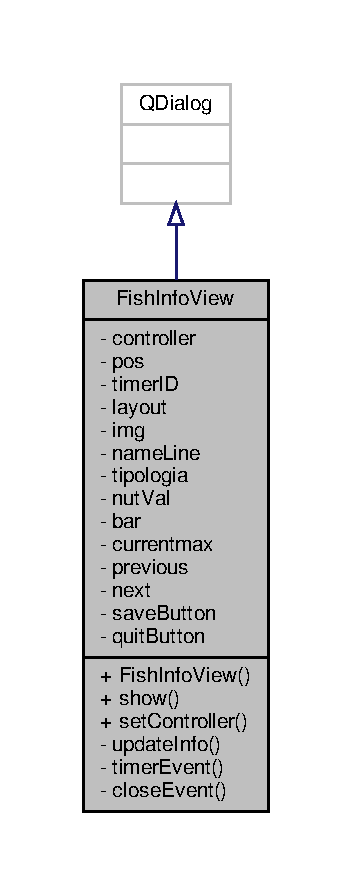
\includegraphics[width=169pt]{classFishInfoView__inherit__graph}
\end{center}
\end{figure}


Collaboration diagram for Fish\+Info\+View\+:\nopagebreak
\begin{figure}[H]
\begin{center}
\leavevmode
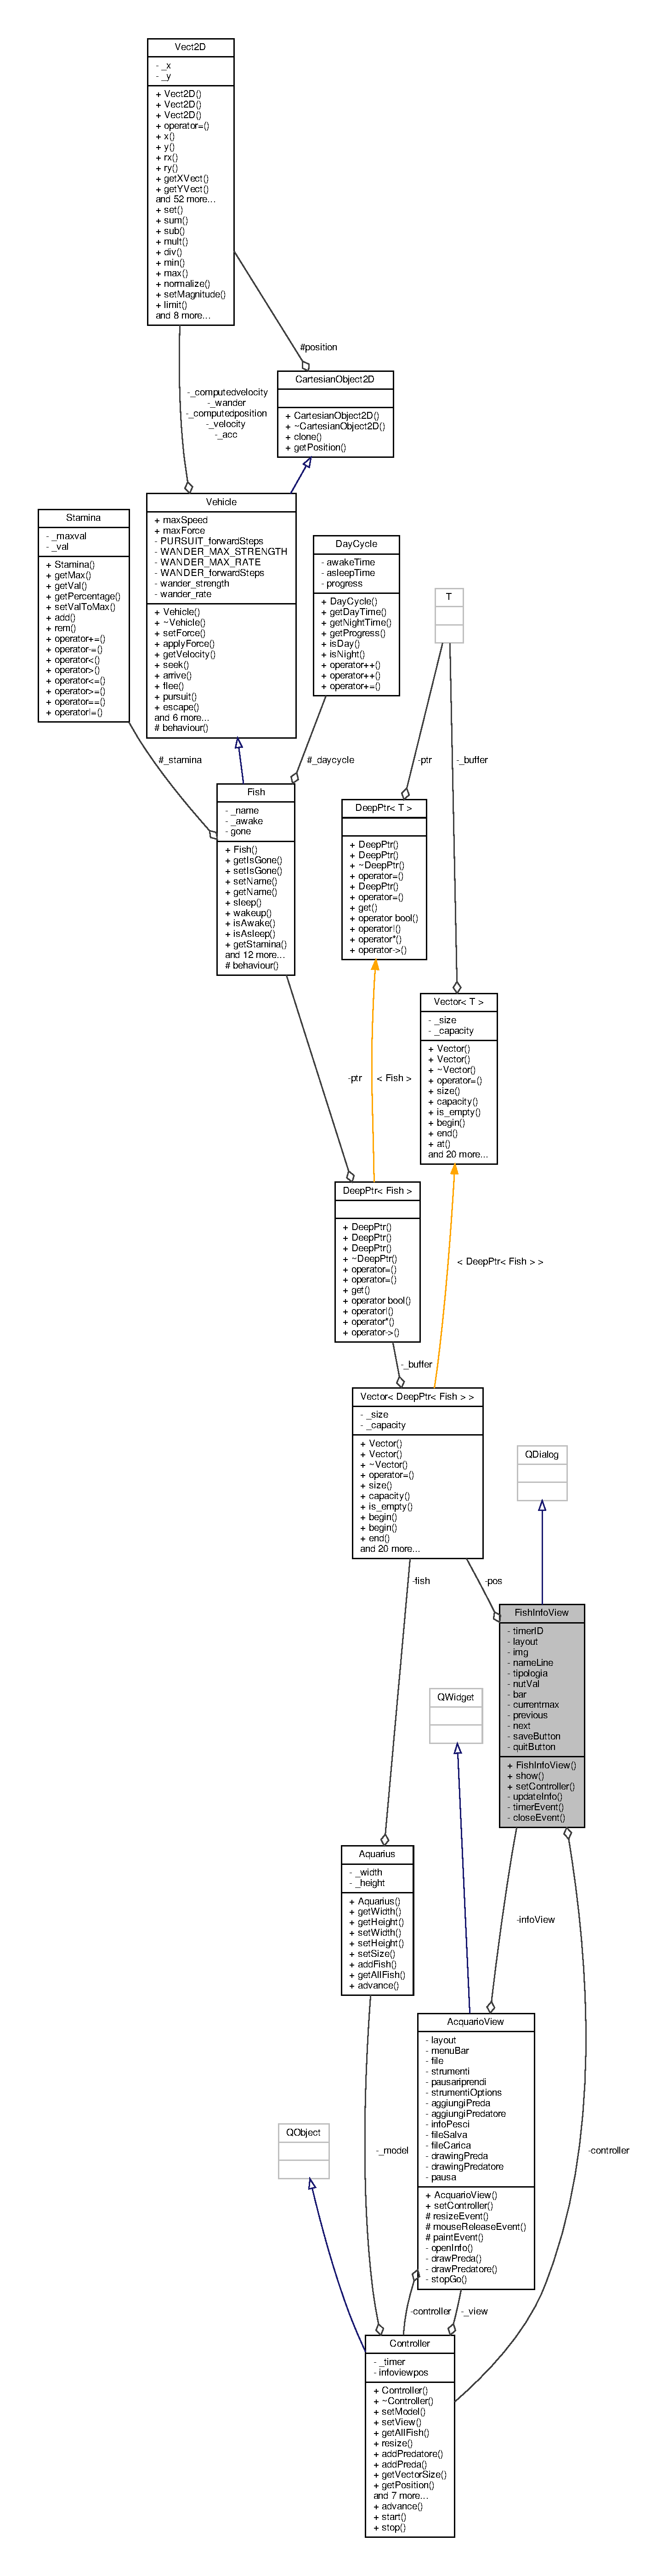
\includegraphics[height=550pt]{classFishInfoView__coll__graph}
\end{center}
\end{figure}
\subsection*{Public Member Functions}
\begin{DoxyCompactItemize}
\item 
\hyperlink{classFishInfoView_aa1baa9e5f073be8bde338beebc4ac209_aa1baa9e5f073be8bde338beebc4ac209}{Fish\+Info\+View} (Q\+Widget $\ast$parent=nullptr)
\item 
void \hyperlink{classFishInfoView_aa4bf1bcf24807044f11a6b22b26431d5_aa4bf1bcf24807044f11a6b22b26431d5}{show} ()
\item 
void \hyperlink{classFishInfoView_ab7dbcbf32286d7f3699cdad3664e7830_ab7dbcbf32286d7f3699cdad3664e7830}{set\+Controller} (\hyperlink{classController}{Controller} $\ast$)
\end{DoxyCompactItemize}
\subsection*{Private Member Functions}
\begin{DoxyCompactItemize}
\item 
void \hyperlink{classFishInfoView_ae789978f20407aed46458af8f3c07aae_ae789978f20407aed46458af8f3c07aae}{update\+Info} ()
\item 
void \hyperlink{classFishInfoView_a5125ab4e284469e0e13438967a6ddfd8_a5125ab4e284469e0e13438967a6ddfd8}{timer\+Event} (Q\+Timer\+Event $\ast$)
\item 
void \hyperlink{classFishInfoView_a0c243d1c712f98879dd6a7f547f30ad0_a0c243d1c712f98879dd6a7f547f30ad0}{close\+Event} (Q\+Close\+Event $\ast$)
\end{DoxyCompactItemize}
\subsection*{Private Attributes}
\begin{DoxyCompactItemize}
\item 
\hyperlink{classController}{Controller} $\ast$ \hyperlink{classFishInfoView_a55d7f45ff776d535d8e9f19f3ab222fb_a55d7f45ff776d535d8e9f19f3ab222fb}{controller}
\item 
\hyperlink{classVector}{Vector}$<$ \hyperlink{classDeepPtr}{Deep\+Ptr}$<$ \hyperlink{classFish}{Fish} $>$ $>$\+::iterator \hyperlink{classFishInfoView_aef313e02efb19ca493e38a670d00031d_aef313e02efb19ca493e38a670d00031d}{pos}
\item 
int \hyperlink{classFishInfoView_a9f28deb4966d0920e59731b01d413379_a9f28deb4966d0920e59731b01d413379}{timer\+ID}
\item 
Q\+Grid\+Layout $\ast$ \hyperlink{classFishInfoView_a5e6524166611597c5cf026cce623e0b5_a5e6524166611597c5cf026cce623e0b5}{layout}
\item 
Q\+Label $\ast$ \hyperlink{classFishInfoView_a042e425491ce018a58ce8eb57f52b19e_a042e425491ce018a58ce8eb57f52b19e}{img}
\item 
Q\+Line\+Edit $\ast$ \hyperlink{classFishInfoView_ade293fb24ac7424ce5bde859f0358c70_ade293fb24ac7424ce5bde859f0358c70}{name\+Line}
\item 
Q\+Label $\ast$ \hyperlink{classFishInfoView_a11aef88bcc65dde952faf47608712738_a11aef88bcc65dde952faf47608712738}{tipologia}
\item 
Q\+Label $\ast$ \hyperlink{classFishInfoView_adaa7f10c903bbe239d619bd86b1b98f5_adaa7f10c903bbe239d619bd86b1b98f5}{nut\+Val}
\item 
Q\+Progress\+Bar $\ast$ \hyperlink{classFishInfoView_a8aad7d3739b1163cacd402ae4cdf47f3_a8aad7d3739b1163cacd402ae4cdf47f3}{bar}
\item 
Q\+Label $\ast$ \hyperlink{classFishInfoView_a9642ead7f4c184cc45556ec8c7346360_a9642ead7f4c184cc45556ec8c7346360}{currentmax}
\item 
Q\+Push\+Button $\ast$ \hyperlink{classFishInfoView_ad22f1d85269cb0dcd7e93eee334bcfc4_ad22f1d85269cb0dcd7e93eee334bcfc4}{previous}
\item 
Q\+Push\+Button $\ast$ \hyperlink{classFishInfoView_aab50a28d3c4ff2e4879f2f4b539aafa5_aab50a28d3c4ff2e4879f2f4b539aafa5}{next}
\item 
Q\+Push\+Button $\ast$ \hyperlink{classFishInfoView_ab28f33062ed6675b3fbb6a79f4d5caa3_ab28f33062ed6675b3fbb6a79f4d5caa3}{save\+Button}
\item 
Q\+Push\+Button $\ast$ \hyperlink{classFishInfoView_a3e7e3f83d45132ee69dcaf3f7e73de93_a3e7e3f83d45132ee69dcaf3f7e73de93}{quit\+Button}
\end{DoxyCompactItemize}


\subsection{Constructor \& Destructor Documentation}
\mbox{\Hypertarget{classFishInfoView_aa1baa9e5f073be8bde338beebc4ac209_aa1baa9e5f073be8bde338beebc4ac209}\label{classFishInfoView_aa1baa9e5f073be8bde338beebc4ac209_aa1baa9e5f073be8bde338beebc4ac209}} 
\index{Fish\+Info\+View@{Fish\+Info\+View}!Fish\+Info\+View@{Fish\+Info\+View}}
\index{Fish\+Info\+View@{Fish\+Info\+View}!Fish\+Info\+View@{Fish\+Info\+View}}
\subsubsection{\texorpdfstring{Fish\+Info\+View()}{FishInfoView()}}
{\footnotesize\ttfamily Fish\+Info\+View\+::\+Fish\+Info\+View (\begin{DoxyParamCaption}\item[{Q\+Widget $\ast$}]{parent = {\ttfamily nullptr} }\end{DoxyParamCaption})}



\subsection{Member Function Documentation}
\mbox{\Hypertarget{classFishInfoView_a0c243d1c712f98879dd6a7f547f30ad0_a0c243d1c712f98879dd6a7f547f30ad0}\label{classFishInfoView_a0c243d1c712f98879dd6a7f547f30ad0_a0c243d1c712f98879dd6a7f547f30ad0}} 
\index{Fish\+Info\+View@{Fish\+Info\+View}!close\+Event@{close\+Event}}
\index{close\+Event@{close\+Event}!Fish\+Info\+View@{Fish\+Info\+View}}
\subsubsection{\texorpdfstring{close\+Event()}{closeEvent()}}
{\footnotesize\ttfamily void Fish\+Info\+View\+::close\+Event (\begin{DoxyParamCaption}\item[{Q\+Close\+Event $\ast$}]{ }\end{DoxyParamCaption})\hspace{0.3cm}{\ttfamily [private]}}

\mbox{\Hypertarget{classFishInfoView_ab7dbcbf32286d7f3699cdad3664e7830_ab7dbcbf32286d7f3699cdad3664e7830}\label{classFishInfoView_ab7dbcbf32286d7f3699cdad3664e7830_ab7dbcbf32286d7f3699cdad3664e7830}} 
\index{Fish\+Info\+View@{Fish\+Info\+View}!set\+Controller@{set\+Controller}}
\index{set\+Controller@{set\+Controller}!Fish\+Info\+View@{Fish\+Info\+View}}
\subsubsection{\texorpdfstring{set\+Controller()}{setController()}}
{\footnotesize\ttfamily void Fish\+Info\+View\+::set\+Controller (\begin{DoxyParamCaption}\item[{\hyperlink{classController}{Controller} $\ast$}]{c }\end{DoxyParamCaption})}

\mbox{\Hypertarget{classFishInfoView_aa4bf1bcf24807044f11a6b22b26431d5_aa4bf1bcf24807044f11a6b22b26431d5}\label{classFishInfoView_aa4bf1bcf24807044f11a6b22b26431d5_aa4bf1bcf24807044f11a6b22b26431d5}} 
\index{Fish\+Info\+View@{Fish\+Info\+View}!show@{show}}
\index{show@{show}!Fish\+Info\+View@{Fish\+Info\+View}}
\subsubsection{\texorpdfstring{show()}{show()}}
{\footnotesize\ttfamily void Fish\+Info\+View\+::show (\begin{DoxyParamCaption}{ }\end{DoxyParamCaption})}

\mbox{\Hypertarget{classFishInfoView_a5125ab4e284469e0e13438967a6ddfd8_a5125ab4e284469e0e13438967a6ddfd8}\label{classFishInfoView_a5125ab4e284469e0e13438967a6ddfd8_a5125ab4e284469e0e13438967a6ddfd8}} 
\index{Fish\+Info\+View@{Fish\+Info\+View}!timer\+Event@{timer\+Event}}
\index{timer\+Event@{timer\+Event}!Fish\+Info\+View@{Fish\+Info\+View}}
\subsubsection{\texorpdfstring{timer\+Event()}{timerEvent()}}
{\footnotesize\ttfamily void Fish\+Info\+View\+::timer\+Event (\begin{DoxyParamCaption}\item[{Q\+Timer\+Event $\ast$}]{ }\end{DoxyParamCaption})\hspace{0.3cm}{\ttfamily [private]}}

\mbox{\Hypertarget{classFishInfoView_ae789978f20407aed46458af8f3c07aae_ae789978f20407aed46458af8f3c07aae}\label{classFishInfoView_ae789978f20407aed46458af8f3c07aae_ae789978f20407aed46458af8f3c07aae}} 
\index{Fish\+Info\+View@{Fish\+Info\+View}!update\+Info@{update\+Info}}
\index{update\+Info@{update\+Info}!Fish\+Info\+View@{Fish\+Info\+View}}
\subsubsection{\texorpdfstring{update\+Info()}{updateInfo()}}
{\footnotesize\ttfamily void Fish\+Info\+View\+::update\+Info (\begin{DoxyParamCaption}{ }\end{DoxyParamCaption})\hspace{0.3cm}{\ttfamily [private]}}



\subsection{Member Data Documentation}
\mbox{\Hypertarget{classFishInfoView_a8aad7d3739b1163cacd402ae4cdf47f3_a8aad7d3739b1163cacd402ae4cdf47f3}\label{classFishInfoView_a8aad7d3739b1163cacd402ae4cdf47f3_a8aad7d3739b1163cacd402ae4cdf47f3}} 
\index{Fish\+Info\+View@{Fish\+Info\+View}!bar@{bar}}
\index{bar@{bar}!Fish\+Info\+View@{Fish\+Info\+View}}
\subsubsection{\texorpdfstring{bar}{bar}}
{\footnotesize\ttfamily Q\+Progress\+Bar$\ast$ Fish\+Info\+View\+::bar\hspace{0.3cm}{\ttfamily [private]}}

\mbox{\Hypertarget{classFishInfoView_a55d7f45ff776d535d8e9f19f3ab222fb_a55d7f45ff776d535d8e9f19f3ab222fb}\label{classFishInfoView_a55d7f45ff776d535d8e9f19f3ab222fb_a55d7f45ff776d535d8e9f19f3ab222fb}} 
\index{Fish\+Info\+View@{Fish\+Info\+View}!controller@{controller}}
\index{controller@{controller}!Fish\+Info\+View@{Fish\+Info\+View}}
\subsubsection{\texorpdfstring{controller}{controller}}
{\footnotesize\ttfamily \hyperlink{classController}{Controller}$\ast$ Fish\+Info\+View\+::controller\hspace{0.3cm}{\ttfamily [private]}}

\mbox{\Hypertarget{classFishInfoView_a9642ead7f4c184cc45556ec8c7346360_a9642ead7f4c184cc45556ec8c7346360}\label{classFishInfoView_a9642ead7f4c184cc45556ec8c7346360_a9642ead7f4c184cc45556ec8c7346360}} 
\index{Fish\+Info\+View@{Fish\+Info\+View}!currentmax@{currentmax}}
\index{currentmax@{currentmax}!Fish\+Info\+View@{Fish\+Info\+View}}
\subsubsection{\texorpdfstring{currentmax}{currentmax}}
{\footnotesize\ttfamily Q\+Label$\ast$ Fish\+Info\+View\+::currentmax\hspace{0.3cm}{\ttfamily [private]}}

\mbox{\Hypertarget{classFishInfoView_a042e425491ce018a58ce8eb57f52b19e_a042e425491ce018a58ce8eb57f52b19e}\label{classFishInfoView_a042e425491ce018a58ce8eb57f52b19e_a042e425491ce018a58ce8eb57f52b19e}} 
\index{Fish\+Info\+View@{Fish\+Info\+View}!img@{img}}
\index{img@{img}!Fish\+Info\+View@{Fish\+Info\+View}}
\subsubsection{\texorpdfstring{img}{img}}
{\footnotesize\ttfamily Q\+Label$\ast$ Fish\+Info\+View\+::img\hspace{0.3cm}{\ttfamily [private]}}

\mbox{\Hypertarget{classFishInfoView_a5e6524166611597c5cf026cce623e0b5_a5e6524166611597c5cf026cce623e0b5}\label{classFishInfoView_a5e6524166611597c5cf026cce623e0b5_a5e6524166611597c5cf026cce623e0b5}} 
\index{Fish\+Info\+View@{Fish\+Info\+View}!layout@{layout}}
\index{layout@{layout}!Fish\+Info\+View@{Fish\+Info\+View}}
\subsubsection{\texorpdfstring{layout}{layout}}
{\footnotesize\ttfamily Q\+Grid\+Layout$\ast$ Fish\+Info\+View\+::layout\hspace{0.3cm}{\ttfamily [private]}}

\mbox{\Hypertarget{classFishInfoView_ade293fb24ac7424ce5bde859f0358c70_ade293fb24ac7424ce5bde859f0358c70}\label{classFishInfoView_ade293fb24ac7424ce5bde859f0358c70_ade293fb24ac7424ce5bde859f0358c70}} 
\index{Fish\+Info\+View@{Fish\+Info\+View}!name\+Line@{name\+Line}}
\index{name\+Line@{name\+Line}!Fish\+Info\+View@{Fish\+Info\+View}}
\subsubsection{\texorpdfstring{name\+Line}{nameLine}}
{\footnotesize\ttfamily Q\+Line\+Edit$\ast$ Fish\+Info\+View\+::name\+Line\hspace{0.3cm}{\ttfamily [private]}}

\mbox{\Hypertarget{classFishInfoView_aab50a28d3c4ff2e4879f2f4b539aafa5_aab50a28d3c4ff2e4879f2f4b539aafa5}\label{classFishInfoView_aab50a28d3c4ff2e4879f2f4b539aafa5_aab50a28d3c4ff2e4879f2f4b539aafa5}} 
\index{Fish\+Info\+View@{Fish\+Info\+View}!next@{next}}
\index{next@{next}!Fish\+Info\+View@{Fish\+Info\+View}}
\subsubsection{\texorpdfstring{next}{next}}
{\footnotesize\ttfamily Q\+Push\+Button$\ast$ Fish\+Info\+View\+::next\hspace{0.3cm}{\ttfamily [private]}}

\mbox{\Hypertarget{classFishInfoView_adaa7f10c903bbe239d619bd86b1b98f5_adaa7f10c903bbe239d619bd86b1b98f5}\label{classFishInfoView_adaa7f10c903bbe239d619bd86b1b98f5_adaa7f10c903bbe239d619bd86b1b98f5}} 
\index{Fish\+Info\+View@{Fish\+Info\+View}!nut\+Val@{nut\+Val}}
\index{nut\+Val@{nut\+Val}!Fish\+Info\+View@{Fish\+Info\+View}}
\subsubsection{\texorpdfstring{nut\+Val}{nutVal}}
{\footnotesize\ttfamily Q\+Label$\ast$ Fish\+Info\+View\+::nut\+Val\hspace{0.3cm}{\ttfamily [private]}}

\mbox{\Hypertarget{classFishInfoView_aef313e02efb19ca493e38a670d00031d_aef313e02efb19ca493e38a670d00031d}\label{classFishInfoView_aef313e02efb19ca493e38a670d00031d_aef313e02efb19ca493e38a670d00031d}} 
\index{Fish\+Info\+View@{Fish\+Info\+View}!pos@{pos}}
\index{pos@{pos}!Fish\+Info\+View@{Fish\+Info\+View}}
\subsubsection{\texorpdfstring{pos}{pos}}
{\footnotesize\ttfamily \hyperlink{classVector}{Vector}$<$\hyperlink{classDeepPtr}{Deep\+Ptr}$<$\hyperlink{classFish}{Fish}$>$ $>$\+::iterator Fish\+Info\+View\+::pos\hspace{0.3cm}{\ttfamily [private]}}

\mbox{\Hypertarget{classFishInfoView_ad22f1d85269cb0dcd7e93eee334bcfc4_ad22f1d85269cb0dcd7e93eee334bcfc4}\label{classFishInfoView_ad22f1d85269cb0dcd7e93eee334bcfc4_ad22f1d85269cb0dcd7e93eee334bcfc4}} 
\index{Fish\+Info\+View@{Fish\+Info\+View}!previous@{previous}}
\index{previous@{previous}!Fish\+Info\+View@{Fish\+Info\+View}}
\subsubsection{\texorpdfstring{previous}{previous}}
{\footnotesize\ttfamily Q\+Push\+Button$\ast$ Fish\+Info\+View\+::previous\hspace{0.3cm}{\ttfamily [private]}}

\mbox{\Hypertarget{classFishInfoView_a3e7e3f83d45132ee69dcaf3f7e73de93_a3e7e3f83d45132ee69dcaf3f7e73de93}\label{classFishInfoView_a3e7e3f83d45132ee69dcaf3f7e73de93_a3e7e3f83d45132ee69dcaf3f7e73de93}} 
\index{Fish\+Info\+View@{Fish\+Info\+View}!quit\+Button@{quit\+Button}}
\index{quit\+Button@{quit\+Button}!Fish\+Info\+View@{Fish\+Info\+View}}
\subsubsection{\texorpdfstring{quit\+Button}{quitButton}}
{\footnotesize\ttfamily Q\+Push\+Button$\ast$ Fish\+Info\+View\+::quit\+Button\hspace{0.3cm}{\ttfamily [private]}}

\mbox{\Hypertarget{classFishInfoView_ab28f33062ed6675b3fbb6a79f4d5caa3_ab28f33062ed6675b3fbb6a79f4d5caa3}\label{classFishInfoView_ab28f33062ed6675b3fbb6a79f4d5caa3_ab28f33062ed6675b3fbb6a79f4d5caa3}} 
\index{Fish\+Info\+View@{Fish\+Info\+View}!save\+Button@{save\+Button}}
\index{save\+Button@{save\+Button}!Fish\+Info\+View@{Fish\+Info\+View}}
\subsubsection{\texorpdfstring{save\+Button}{saveButton}}
{\footnotesize\ttfamily Q\+Push\+Button$\ast$ Fish\+Info\+View\+::save\+Button\hspace{0.3cm}{\ttfamily [private]}}

\mbox{\Hypertarget{classFishInfoView_a9f28deb4966d0920e59731b01d413379_a9f28deb4966d0920e59731b01d413379}\label{classFishInfoView_a9f28deb4966d0920e59731b01d413379_a9f28deb4966d0920e59731b01d413379}} 
\index{Fish\+Info\+View@{Fish\+Info\+View}!timer\+ID@{timer\+ID}}
\index{timer\+ID@{timer\+ID}!Fish\+Info\+View@{Fish\+Info\+View}}
\subsubsection{\texorpdfstring{timer\+ID}{timerID}}
{\footnotesize\ttfamily int Fish\+Info\+View\+::timer\+ID\hspace{0.3cm}{\ttfamily [private]}}

\mbox{\Hypertarget{classFishInfoView_a11aef88bcc65dde952faf47608712738_a11aef88bcc65dde952faf47608712738}\label{classFishInfoView_a11aef88bcc65dde952faf47608712738_a11aef88bcc65dde952faf47608712738}} 
\index{Fish\+Info\+View@{Fish\+Info\+View}!tipologia@{tipologia}}
\index{tipologia@{tipologia}!Fish\+Info\+View@{Fish\+Info\+View}}
\subsubsection{\texorpdfstring{tipologia}{tipologia}}
{\footnotesize\ttfamily Q\+Label$\ast$ Fish\+Info\+View\+::tipologia\hspace{0.3cm}{\ttfamily [private]}}



The documentation for this class was generated from the following files\+:\begin{DoxyCompactItemize}
\item 
include/\hyperlink{fishinfoview_8hpp}{fishinfoview.\+hpp}\item 
src/\hyperlink{fishinfoview_8cpp}{fishinfoview.\+cpp}\end{DoxyCompactItemize}

\hypertarget{classVector_1_1iterator}{}\section{Vector$<$ T $>$\+:\+:iterator Class Reference}
\label{classVector_1_1iterator}\index{Vector$<$ T $>$\+::iterator@{Vector$<$ T $>$\+::iterator}}


{\ttfamily \#include $<$vector.\+hpp$>$}



Collaboration diagram for Vector$<$ T $>$\+:\+:iterator\+:\nopagebreak
\begin{figure}[H]
\begin{center}
\leavevmode
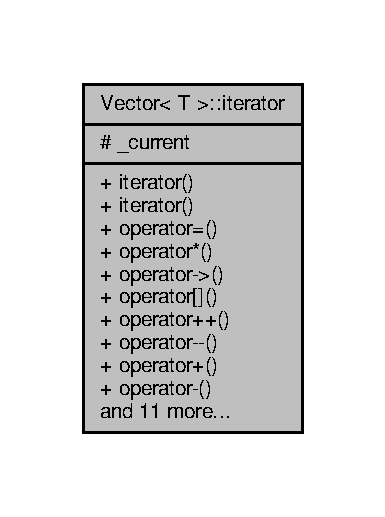
\includegraphics[width=185pt]{classVector_1_1iterator__coll__graph}
\end{center}
\end{figure}
\subsection*{Public Member Functions}
\begin{DoxyCompactItemize}
\item 
\hyperlink{classVector_1_1iterator_ac19ddeac03f06dfa9409375a389dc6b6_ac19ddeac03f06dfa9409375a389dc6b6}{iterator} (T $\ast$i=nullptr)
\item 
\hyperlink{classVector_1_1iterator_a824de93327bac2821ce81d67aa097436_a824de93327bac2821ce81d67aa097436}{iterator} (const \hyperlink{classVector_1_1iterator}{iterator} \&i)
\item 
\hyperlink{classVector_1_1iterator}{iterator} \& \hyperlink{classVector_1_1iterator_a872f28a0c1c29c65ff093a11723fb1a0_a872f28a0c1c29c65ff093a11723fb1a0}{operator=} (const \hyperlink{classVector_1_1iterator}{iterator} \&i)
\item 
T \& \hyperlink{classVector_1_1iterator_a55aa58a9c5917f66b6c2d57617e67036_a55aa58a9c5917f66b6c2d57617e67036}{operator$\ast$} () const
\item 
T $\ast$ \hyperlink{classVector_1_1iterator_a9ead9fe946e057e6d423d9c07b9439c4_a9ead9fe946e057e6d423d9c07b9439c4}{operator-\/$>$} () const
\item 
T \& \hyperlink{classVector_1_1iterator_ab317050a91c9bbc9cb3395824891c36c_ab317050a91c9bbc9cb3395824891c36c}{operator\mbox{[}$\,$\mbox{]}} (int n) const
\item 
\hyperlink{classVector_1_1iterator}{iterator} \hyperlink{classVector_1_1iterator_ac67c9225a0971d334d02246291922539_ac67c9225a0971d334d02246291922539}{operator++} (int)
\item 
\hyperlink{classVector_1_1iterator}{iterator} \hyperlink{classVector_1_1iterator_a4bbb51eb646080bf397665d903ad94d7_a4bbb51eb646080bf397665d903ad94d7}{operator-\/-\/} (int)
\item 
\hyperlink{classVector_1_1iterator}{iterator} \hyperlink{classVector_1_1iterator_ae04a470594c8475c04e229cd8711b585_ae04a470594c8475c04e229cd8711b585}{operator+} (int n) const
\item 
\hyperlink{classVector_1_1iterator}{iterator} \hyperlink{classVector_1_1iterator_a47db88e770bfa09969c5942b09c24c46_a47db88e770bfa09969c5942b09c24c46}{operator-\/} (int n) const
\item 
\hyperlink{classVector_1_1iterator}{iterator} \& \hyperlink{classVector_1_1iterator_a5016f39ffd22095b6fa9de87a5dac20e_a5016f39ffd22095b6fa9de87a5dac20e}{operator++} ()
\item 
\hyperlink{classVector_1_1iterator}{iterator} \& \hyperlink{classVector_1_1iterator_ac2a3f19d49c56b74100ac758cc5fc2aa_ac2a3f19d49c56b74100ac758cc5fc2aa}{operator-\/-\/} ()
\item 
\hyperlink{classVector_1_1iterator}{iterator} \& \hyperlink{classVector_1_1iterator_a5bf29b945b7717ff57ac278f7de6c158_a5bf29b945b7717ff57ac278f7de6c158}{operator+=} (int n)
\item 
\hyperlink{classVector_1_1iterator}{iterator} \& \hyperlink{classVector_1_1iterator_a51446f7c5ebf3c37db5f2855217836b6_a51446f7c5ebf3c37db5f2855217836b6}{operator-\/=} (int n)
\item 
\hyperlink{classVector_1_1iterator_a19a200b30d6acf43210a44620462e5e8_a19a200b30d6acf43210a44620462e5e8}{operator const\+\_\+iterator} ()
\item 
bool \hyperlink{classVector_1_1iterator_a105d376582ed6fdbf2e645f95a3b26df_a105d376582ed6fdbf2e645f95a3b26df}{operator==} (const \hyperlink{classVector_1_1iterator}{iterator} \&i) const
\item 
bool \hyperlink{classVector_1_1iterator_a755741485c5a92ed32484b350abfd041_a755741485c5a92ed32484b350abfd041}{operator!=} (const \hyperlink{classVector_1_1iterator}{iterator} \&i) const
\item 
bool \hyperlink{classVector_1_1iterator_a2168ad507f6877bd555bb00094eae2a7_a2168ad507f6877bd555bb00094eae2a7}{operator$<$} (const \hyperlink{classVector_1_1iterator}{iterator} \&i) const
\item 
bool \hyperlink{classVector_1_1iterator_a1136d388a7615e1b924ae5e30db1e420_a1136d388a7615e1b924ae5e30db1e420}{operator$>$} (const \hyperlink{classVector_1_1iterator}{iterator} \&i) const
\item 
bool \hyperlink{classVector_1_1iterator_af74c57313919fde4c919027969233977_af74c57313919fde4c919027969233977}{operator$<$=} (const \hyperlink{classVector_1_1iterator}{iterator} \&i) const
\item 
bool \hyperlink{classVector_1_1iterator_ae7d6040f2120fcb90582dafe924e837b_ae7d6040f2120fcb90582dafe924e837b}{operator$>$=} (const \hyperlink{classVector_1_1iterator}{iterator} \&i) const
\end{DoxyCompactItemize}
\subsection*{Protected Attributes}
\begin{DoxyCompactItemize}
\item 
T $\ast$ \hyperlink{classVector_1_1iterator_a4631750ea2c5b6a421b0d0eedbe4627c_a4631750ea2c5b6a421b0d0eedbe4627c}{\+\_\+current}
\end{DoxyCompactItemize}


\subsection{Constructor \& Destructor Documentation}
\mbox{\Hypertarget{classVector_1_1iterator_ac19ddeac03f06dfa9409375a389dc6b6_ac19ddeac03f06dfa9409375a389dc6b6}\label{classVector_1_1iterator_ac19ddeac03f06dfa9409375a389dc6b6_ac19ddeac03f06dfa9409375a389dc6b6}} 
\index{Vector\+::iterator@{Vector\+::iterator}!iterator@{iterator}}
\index{iterator@{iterator}!Vector\+::iterator@{Vector\+::iterator}}
\subsubsection{\texorpdfstring{iterator()}{iterator()}\hspace{0.1cm}{\footnotesize\ttfamily [1/2]}}
{\footnotesize\ttfamily template$<$class T$>$ \\
\hyperlink{classVector}{Vector}$<$ T $>$\+::iterator\+::iterator (\begin{DoxyParamCaption}\item[{T $\ast$}]{i = {\ttfamily nullptr} }\end{DoxyParamCaption})\hspace{0.3cm}{\ttfamily [inline]}}

\mbox{\Hypertarget{classVector_1_1iterator_a824de93327bac2821ce81d67aa097436_a824de93327bac2821ce81d67aa097436}\label{classVector_1_1iterator_a824de93327bac2821ce81d67aa097436_a824de93327bac2821ce81d67aa097436}} 
\index{Vector\+::iterator@{Vector\+::iterator}!iterator@{iterator}}
\index{iterator@{iterator}!Vector\+::iterator@{Vector\+::iterator}}
\subsubsection{\texorpdfstring{iterator()}{iterator()}\hspace{0.1cm}{\footnotesize\ttfamily [2/2]}}
{\footnotesize\ttfamily template$<$class T$>$ \\
\hyperlink{classVector}{Vector}$<$ T $>$\+::iterator\+::iterator (\begin{DoxyParamCaption}\item[{const \hyperlink{classVector_1_1iterator}{iterator} \&}]{i }\end{DoxyParamCaption})\hspace{0.3cm}{\ttfamily [inline]}}



\subsection{Member Function Documentation}
\mbox{\Hypertarget{classVector_1_1iterator_a19a200b30d6acf43210a44620462e5e8_a19a200b30d6acf43210a44620462e5e8}\label{classVector_1_1iterator_a19a200b30d6acf43210a44620462e5e8_a19a200b30d6acf43210a44620462e5e8}} 
\index{Vector\+::iterator@{Vector\+::iterator}!operator const\+\_\+iterator@{operator const\+\_\+iterator}}
\index{operator const\+\_\+iterator@{operator const\+\_\+iterator}!Vector\+::iterator@{Vector\+::iterator}}
\subsubsection{\texorpdfstring{operator const\+\_\+iterator()}{operator const\_iterator()}}
{\footnotesize\ttfamily template$<$class T$>$ \\
\hyperlink{classVector}{Vector}$<$ T $>$\+::iterator\+::operator \hyperlink{classVector_1_1const__iterator}{const\+\_\+iterator} (\begin{DoxyParamCaption}{ }\end{DoxyParamCaption})\hspace{0.3cm}{\ttfamily [inline]}}

\mbox{\Hypertarget{classVector_1_1iterator_a755741485c5a92ed32484b350abfd041_a755741485c5a92ed32484b350abfd041}\label{classVector_1_1iterator_a755741485c5a92ed32484b350abfd041_a755741485c5a92ed32484b350abfd041}} 
\index{Vector\+::iterator@{Vector\+::iterator}!operator"!=@{operator"!=}}
\index{operator"!=@{operator"!=}!Vector\+::iterator@{Vector\+::iterator}}
\subsubsection{\texorpdfstring{operator"!=()}{operator!=()}}
{\footnotesize\ttfamily template$<$class T$>$ \\
bool \hyperlink{classVector}{Vector}$<$ T $>$\+::iterator\+::operator!= (\begin{DoxyParamCaption}\item[{const \hyperlink{classVector_1_1iterator}{iterator} \&}]{i }\end{DoxyParamCaption}) const\hspace{0.3cm}{\ttfamily [inline]}}

\mbox{\Hypertarget{classVector_1_1iterator_a55aa58a9c5917f66b6c2d57617e67036_a55aa58a9c5917f66b6c2d57617e67036}\label{classVector_1_1iterator_a55aa58a9c5917f66b6c2d57617e67036_a55aa58a9c5917f66b6c2d57617e67036}} 
\index{Vector\+::iterator@{Vector\+::iterator}!operator$\ast$@{operator$\ast$}}
\index{operator$\ast$@{operator$\ast$}!Vector\+::iterator@{Vector\+::iterator}}
\subsubsection{\texorpdfstring{operator$\ast$()}{operator*()}}
{\footnotesize\ttfamily template$<$class T$>$ \\
T\& \hyperlink{classVector}{Vector}$<$ T $>$\+::iterator\+::operator$\ast$ (\begin{DoxyParamCaption}{ }\end{DoxyParamCaption}) const\hspace{0.3cm}{\ttfamily [inline]}}

\mbox{\Hypertarget{classVector_1_1iterator_ae04a470594c8475c04e229cd8711b585_ae04a470594c8475c04e229cd8711b585}\label{classVector_1_1iterator_ae04a470594c8475c04e229cd8711b585_ae04a470594c8475c04e229cd8711b585}} 
\index{Vector\+::iterator@{Vector\+::iterator}!operator+@{operator+}}
\index{operator+@{operator+}!Vector\+::iterator@{Vector\+::iterator}}
\subsubsection{\texorpdfstring{operator+()}{operator+()}}
{\footnotesize\ttfamily template$<$class T$>$ \\
\hyperlink{classVector_1_1iterator}{iterator} \hyperlink{classVector}{Vector}$<$ T $>$\+::iterator\+::operator+ (\begin{DoxyParamCaption}\item[{int}]{n }\end{DoxyParamCaption}) const\hspace{0.3cm}{\ttfamily [inline]}}

\mbox{\Hypertarget{classVector_1_1iterator_ac67c9225a0971d334d02246291922539_ac67c9225a0971d334d02246291922539}\label{classVector_1_1iterator_ac67c9225a0971d334d02246291922539_ac67c9225a0971d334d02246291922539}} 
\index{Vector\+::iterator@{Vector\+::iterator}!operator++@{operator++}}
\index{operator++@{operator++}!Vector\+::iterator@{Vector\+::iterator}}
\subsubsection{\texorpdfstring{operator++()}{operator++()}\hspace{0.1cm}{\footnotesize\ttfamily [1/2]}}
{\footnotesize\ttfamily template$<$class T$>$ \\
\hyperlink{classVector_1_1iterator}{iterator} \hyperlink{classVector}{Vector}$<$ T $>$\+::iterator\+::operator++ (\begin{DoxyParamCaption}\item[{int}]{ }\end{DoxyParamCaption})\hspace{0.3cm}{\ttfamily [inline]}}

\mbox{\Hypertarget{classVector_1_1iterator_a5016f39ffd22095b6fa9de87a5dac20e_a5016f39ffd22095b6fa9de87a5dac20e}\label{classVector_1_1iterator_a5016f39ffd22095b6fa9de87a5dac20e_a5016f39ffd22095b6fa9de87a5dac20e}} 
\index{Vector\+::iterator@{Vector\+::iterator}!operator++@{operator++}}
\index{operator++@{operator++}!Vector\+::iterator@{Vector\+::iterator}}
\subsubsection{\texorpdfstring{operator++()}{operator++()}\hspace{0.1cm}{\footnotesize\ttfamily [2/2]}}
{\footnotesize\ttfamily template$<$class T$>$ \\
\hyperlink{classVector_1_1iterator}{iterator}\& \hyperlink{classVector}{Vector}$<$ T $>$\+::iterator\+::operator++ (\begin{DoxyParamCaption}{ }\end{DoxyParamCaption})\hspace{0.3cm}{\ttfamily [inline]}}

\mbox{\Hypertarget{classVector_1_1iterator_a5bf29b945b7717ff57ac278f7de6c158_a5bf29b945b7717ff57ac278f7de6c158}\label{classVector_1_1iterator_a5bf29b945b7717ff57ac278f7de6c158_a5bf29b945b7717ff57ac278f7de6c158}} 
\index{Vector\+::iterator@{Vector\+::iterator}!operator+=@{operator+=}}
\index{operator+=@{operator+=}!Vector\+::iterator@{Vector\+::iterator}}
\subsubsection{\texorpdfstring{operator+=()}{operator+=()}}
{\footnotesize\ttfamily template$<$class T$>$ \\
\hyperlink{classVector_1_1iterator}{iterator}\& \hyperlink{classVector}{Vector}$<$ T $>$\+::iterator\+::operator+= (\begin{DoxyParamCaption}\item[{int}]{n }\end{DoxyParamCaption})\hspace{0.3cm}{\ttfamily [inline]}}

\mbox{\Hypertarget{classVector_1_1iterator_a47db88e770bfa09969c5942b09c24c46_a47db88e770bfa09969c5942b09c24c46}\label{classVector_1_1iterator_a47db88e770bfa09969c5942b09c24c46_a47db88e770bfa09969c5942b09c24c46}} 
\index{Vector\+::iterator@{Vector\+::iterator}!operator-\/@{operator-\/}}
\index{operator-\/@{operator-\/}!Vector\+::iterator@{Vector\+::iterator}}
\subsubsection{\texorpdfstring{operator-\/()}{operator-()}}
{\footnotesize\ttfamily template$<$class T$>$ \\
\hyperlink{classVector_1_1iterator}{iterator} \hyperlink{classVector}{Vector}$<$ T $>$\+::iterator\+::operator-\/ (\begin{DoxyParamCaption}\item[{int}]{n }\end{DoxyParamCaption}) const\hspace{0.3cm}{\ttfamily [inline]}}

\mbox{\Hypertarget{classVector_1_1iterator_a4bbb51eb646080bf397665d903ad94d7_a4bbb51eb646080bf397665d903ad94d7}\label{classVector_1_1iterator_a4bbb51eb646080bf397665d903ad94d7_a4bbb51eb646080bf397665d903ad94d7}} 
\index{Vector\+::iterator@{Vector\+::iterator}!operator-\/-\/@{operator-\/-\/}}
\index{operator-\/-\/@{operator-\/-\/}!Vector\+::iterator@{Vector\+::iterator}}
\subsubsection{\texorpdfstring{operator-\/-\/()}{operator--()}\hspace{0.1cm}{\footnotesize\ttfamily [1/2]}}
{\footnotesize\ttfamily template$<$class T$>$ \\
\hyperlink{classVector_1_1iterator}{iterator} \hyperlink{classVector}{Vector}$<$ T $>$\+::iterator\+::operator-\/-\/ (\begin{DoxyParamCaption}\item[{int}]{ }\end{DoxyParamCaption})\hspace{0.3cm}{\ttfamily [inline]}}

\mbox{\Hypertarget{classVector_1_1iterator_ac2a3f19d49c56b74100ac758cc5fc2aa_ac2a3f19d49c56b74100ac758cc5fc2aa}\label{classVector_1_1iterator_ac2a3f19d49c56b74100ac758cc5fc2aa_ac2a3f19d49c56b74100ac758cc5fc2aa}} 
\index{Vector\+::iterator@{Vector\+::iterator}!operator-\/-\/@{operator-\/-\/}}
\index{operator-\/-\/@{operator-\/-\/}!Vector\+::iterator@{Vector\+::iterator}}
\subsubsection{\texorpdfstring{operator-\/-\/()}{operator--()}\hspace{0.1cm}{\footnotesize\ttfamily [2/2]}}
{\footnotesize\ttfamily template$<$class T$>$ \\
\hyperlink{classVector_1_1iterator}{iterator}\& \hyperlink{classVector}{Vector}$<$ T $>$\+::iterator\+::operator-\/-\/ (\begin{DoxyParamCaption}{ }\end{DoxyParamCaption})\hspace{0.3cm}{\ttfamily [inline]}}

\mbox{\Hypertarget{classVector_1_1iterator_a51446f7c5ebf3c37db5f2855217836b6_a51446f7c5ebf3c37db5f2855217836b6}\label{classVector_1_1iterator_a51446f7c5ebf3c37db5f2855217836b6_a51446f7c5ebf3c37db5f2855217836b6}} 
\index{Vector\+::iterator@{Vector\+::iterator}!operator-\/=@{operator-\/=}}
\index{operator-\/=@{operator-\/=}!Vector\+::iterator@{Vector\+::iterator}}
\subsubsection{\texorpdfstring{operator-\/=()}{operator-=()}}
{\footnotesize\ttfamily template$<$class T$>$ \\
\hyperlink{classVector_1_1iterator}{iterator}\& \hyperlink{classVector}{Vector}$<$ T $>$\+::iterator\+::operator-\/= (\begin{DoxyParamCaption}\item[{int}]{n }\end{DoxyParamCaption})\hspace{0.3cm}{\ttfamily [inline]}}

\mbox{\Hypertarget{classVector_1_1iterator_a9ead9fe946e057e6d423d9c07b9439c4_a9ead9fe946e057e6d423d9c07b9439c4}\label{classVector_1_1iterator_a9ead9fe946e057e6d423d9c07b9439c4_a9ead9fe946e057e6d423d9c07b9439c4}} 
\index{Vector\+::iterator@{Vector\+::iterator}!operator-\/$>$@{operator-\/$>$}}
\index{operator-\/$>$@{operator-\/$>$}!Vector\+::iterator@{Vector\+::iterator}}
\subsubsection{\texorpdfstring{operator-\/$>$()}{operator->()}}
{\footnotesize\ttfamily template$<$class T$>$ \\
T$\ast$ \hyperlink{classVector}{Vector}$<$ T $>$\+::iterator\+::operator-\/$>$ (\begin{DoxyParamCaption}{ }\end{DoxyParamCaption}) const\hspace{0.3cm}{\ttfamily [inline]}}

\mbox{\Hypertarget{classVector_1_1iterator_a2168ad507f6877bd555bb00094eae2a7_a2168ad507f6877bd555bb00094eae2a7}\label{classVector_1_1iterator_a2168ad507f6877bd555bb00094eae2a7_a2168ad507f6877bd555bb00094eae2a7}} 
\index{Vector\+::iterator@{Vector\+::iterator}!operator$<$@{operator$<$}}
\index{operator$<$@{operator$<$}!Vector\+::iterator@{Vector\+::iterator}}
\subsubsection{\texorpdfstring{operator$<$()}{operator<()}}
{\footnotesize\ttfamily template$<$class T$>$ \\
bool \hyperlink{classVector}{Vector}$<$ T $>$\+::iterator\+::operator$<$ (\begin{DoxyParamCaption}\item[{const \hyperlink{classVector_1_1iterator}{iterator} \&}]{i }\end{DoxyParamCaption}) const\hspace{0.3cm}{\ttfamily [inline]}}

\mbox{\Hypertarget{classVector_1_1iterator_af74c57313919fde4c919027969233977_af74c57313919fde4c919027969233977}\label{classVector_1_1iterator_af74c57313919fde4c919027969233977_af74c57313919fde4c919027969233977}} 
\index{Vector\+::iterator@{Vector\+::iterator}!operator$<$=@{operator$<$=}}
\index{operator$<$=@{operator$<$=}!Vector\+::iterator@{Vector\+::iterator}}
\subsubsection{\texorpdfstring{operator$<$=()}{operator<=()}}
{\footnotesize\ttfamily template$<$class T$>$ \\
bool \hyperlink{classVector}{Vector}$<$ T $>$\+::iterator\+::operator$<$= (\begin{DoxyParamCaption}\item[{const \hyperlink{classVector_1_1iterator}{iterator} \&}]{i }\end{DoxyParamCaption}) const\hspace{0.3cm}{\ttfamily [inline]}}

\mbox{\Hypertarget{classVector_1_1iterator_a872f28a0c1c29c65ff093a11723fb1a0_a872f28a0c1c29c65ff093a11723fb1a0}\label{classVector_1_1iterator_a872f28a0c1c29c65ff093a11723fb1a0_a872f28a0c1c29c65ff093a11723fb1a0}} 
\index{Vector\+::iterator@{Vector\+::iterator}!operator=@{operator=}}
\index{operator=@{operator=}!Vector\+::iterator@{Vector\+::iterator}}
\subsubsection{\texorpdfstring{operator=()}{operator=()}}
{\footnotesize\ttfamily template$<$class T$>$ \\
\hyperlink{classVector_1_1iterator}{iterator}\& \hyperlink{classVector}{Vector}$<$ T $>$\+::iterator\+::operator= (\begin{DoxyParamCaption}\item[{const \hyperlink{classVector_1_1iterator}{iterator} \&}]{i }\end{DoxyParamCaption})\hspace{0.3cm}{\ttfamily [inline]}}

\mbox{\Hypertarget{classVector_1_1iterator_a105d376582ed6fdbf2e645f95a3b26df_a105d376582ed6fdbf2e645f95a3b26df}\label{classVector_1_1iterator_a105d376582ed6fdbf2e645f95a3b26df_a105d376582ed6fdbf2e645f95a3b26df}} 
\index{Vector\+::iterator@{Vector\+::iterator}!operator==@{operator==}}
\index{operator==@{operator==}!Vector\+::iterator@{Vector\+::iterator}}
\subsubsection{\texorpdfstring{operator==()}{operator==()}}
{\footnotesize\ttfamily template$<$class T$>$ \\
bool \hyperlink{classVector}{Vector}$<$ T $>$\+::iterator\+::operator== (\begin{DoxyParamCaption}\item[{const \hyperlink{classVector_1_1iterator}{iterator} \&}]{i }\end{DoxyParamCaption}) const\hspace{0.3cm}{\ttfamily [inline]}}

\mbox{\Hypertarget{classVector_1_1iterator_a1136d388a7615e1b924ae5e30db1e420_a1136d388a7615e1b924ae5e30db1e420}\label{classVector_1_1iterator_a1136d388a7615e1b924ae5e30db1e420_a1136d388a7615e1b924ae5e30db1e420}} 
\index{Vector\+::iterator@{Vector\+::iterator}!operator$>$@{operator$>$}}
\index{operator$>$@{operator$>$}!Vector\+::iterator@{Vector\+::iterator}}
\subsubsection{\texorpdfstring{operator$>$()}{operator>()}}
{\footnotesize\ttfamily template$<$class T$>$ \\
bool \hyperlink{classVector}{Vector}$<$ T $>$\+::iterator\+::operator$>$ (\begin{DoxyParamCaption}\item[{const \hyperlink{classVector_1_1iterator}{iterator} \&}]{i }\end{DoxyParamCaption}) const\hspace{0.3cm}{\ttfamily [inline]}}

\mbox{\Hypertarget{classVector_1_1iterator_ae7d6040f2120fcb90582dafe924e837b_ae7d6040f2120fcb90582dafe924e837b}\label{classVector_1_1iterator_ae7d6040f2120fcb90582dafe924e837b_ae7d6040f2120fcb90582dafe924e837b}} 
\index{Vector\+::iterator@{Vector\+::iterator}!operator$>$=@{operator$>$=}}
\index{operator$>$=@{operator$>$=}!Vector\+::iterator@{Vector\+::iterator}}
\subsubsection{\texorpdfstring{operator$>$=()}{operator>=()}}
{\footnotesize\ttfamily template$<$class T$>$ \\
bool \hyperlink{classVector}{Vector}$<$ T $>$\+::iterator\+::operator$>$= (\begin{DoxyParamCaption}\item[{const \hyperlink{classVector_1_1iterator}{iterator} \&}]{i }\end{DoxyParamCaption}) const\hspace{0.3cm}{\ttfamily [inline]}}

\mbox{\Hypertarget{classVector_1_1iterator_ab317050a91c9bbc9cb3395824891c36c_ab317050a91c9bbc9cb3395824891c36c}\label{classVector_1_1iterator_ab317050a91c9bbc9cb3395824891c36c_ab317050a91c9bbc9cb3395824891c36c}} 
\index{Vector\+::iterator@{Vector\+::iterator}!operator\mbox{[}\mbox{]}@{operator[]}}
\index{operator\mbox{[}\mbox{]}@{operator[]}!Vector\+::iterator@{Vector\+::iterator}}
\subsubsection{\texorpdfstring{operator[]()}{operator[]()}}
{\footnotesize\ttfamily template$<$class T$>$ \\
T\& \hyperlink{classVector}{Vector}$<$ T $>$\+::iterator\+::operator\mbox{[}$\,$\mbox{]} (\begin{DoxyParamCaption}\item[{int}]{n }\end{DoxyParamCaption}) const\hspace{0.3cm}{\ttfamily [inline]}}



\subsection{Member Data Documentation}
\mbox{\Hypertarget{classVector_1_1iterator_a4631750ea2c5b6a421b0d0eedbe4627c_a4631750ea2c5b6a421b0d0eedbe4627c}\label{classVector_1_1iterator_a4631750ea2c5b6a421b0d0eedbe4627c_a4631750ea2c5b6a421b0d0eedbe4627c}} 
\index{Vector\+::iterator@{Vector\+::iterator}!\+\_\+current@{\+\_\+current}}
\index{\+\_\+current@{\+\_\+current}!Vector\+::iterator@{Vector\+::iterator}}
\subsubsection{\texorpdfstring{\+\_\+current}{\_current}}
{\footnotesize\ttfamily template$<$class T$>$ \\
T$\ast$ \hyperlink{classVector}{Vector}$<$ T $>$\+::iterator\+::\+\_\+current\hspace{0.3cm}{\ttfamily [protected]}}



The documentation for this class was generated from the following file\+:\begin{DoxyCompactItemize}
\item 
include/\hyperlink{vector_8hpp}{vector.\+hpp}\end{DoxyCompactItemize}

\hypertarget{classPreda}{}\section{Preda Class Reference}
\label{classPreda}\index{Preda@{Preda}}


{\ttfamily \#include $<$preda.\+hpp$>$}



Inheritance diagram for Preda\+:\nopagebreak
\begin{figure}[H]
\begin{center}
\leavevmode
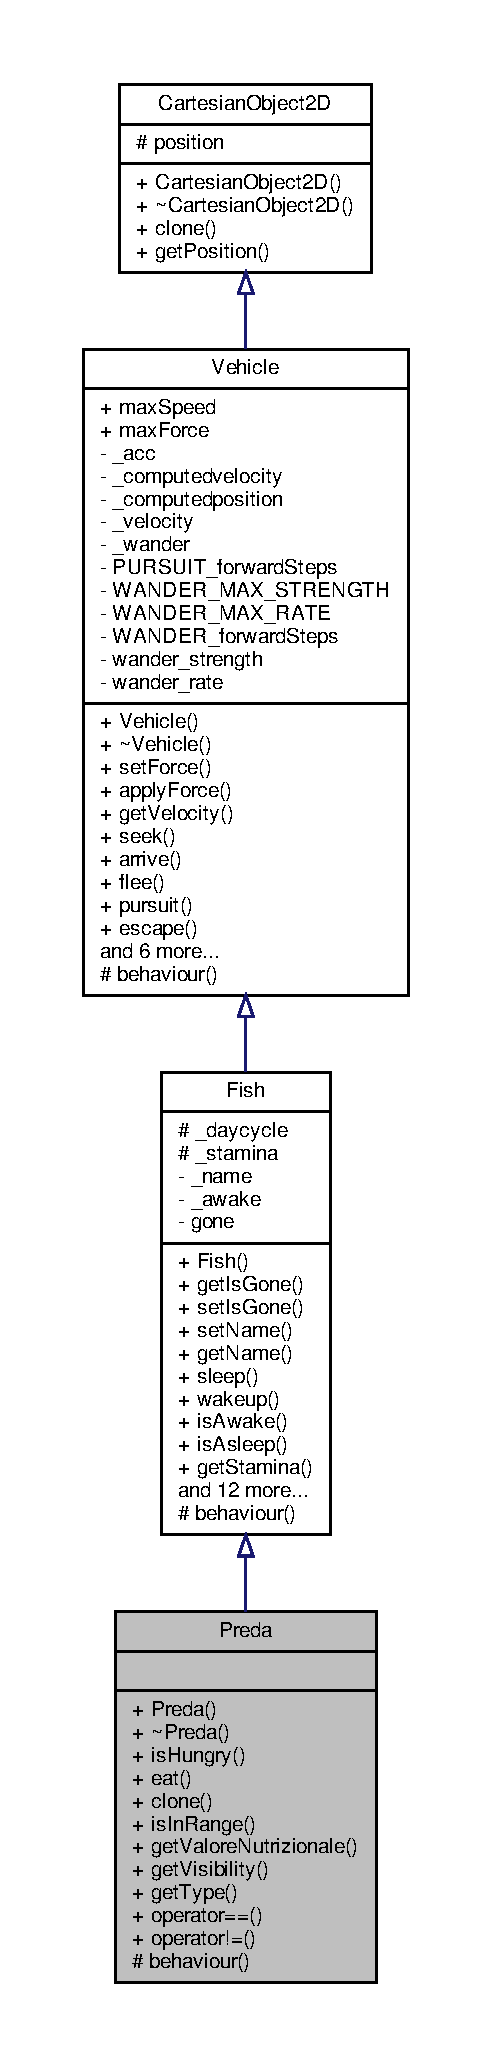
\includegraphics[height=550pt]{classPreda__inherit__graph}
\end{center}
\end{figure}


Collaboration diagram for Preda\+:\nopagebreak
\begin{figure}[H]
\begin{center}
\leavevmode
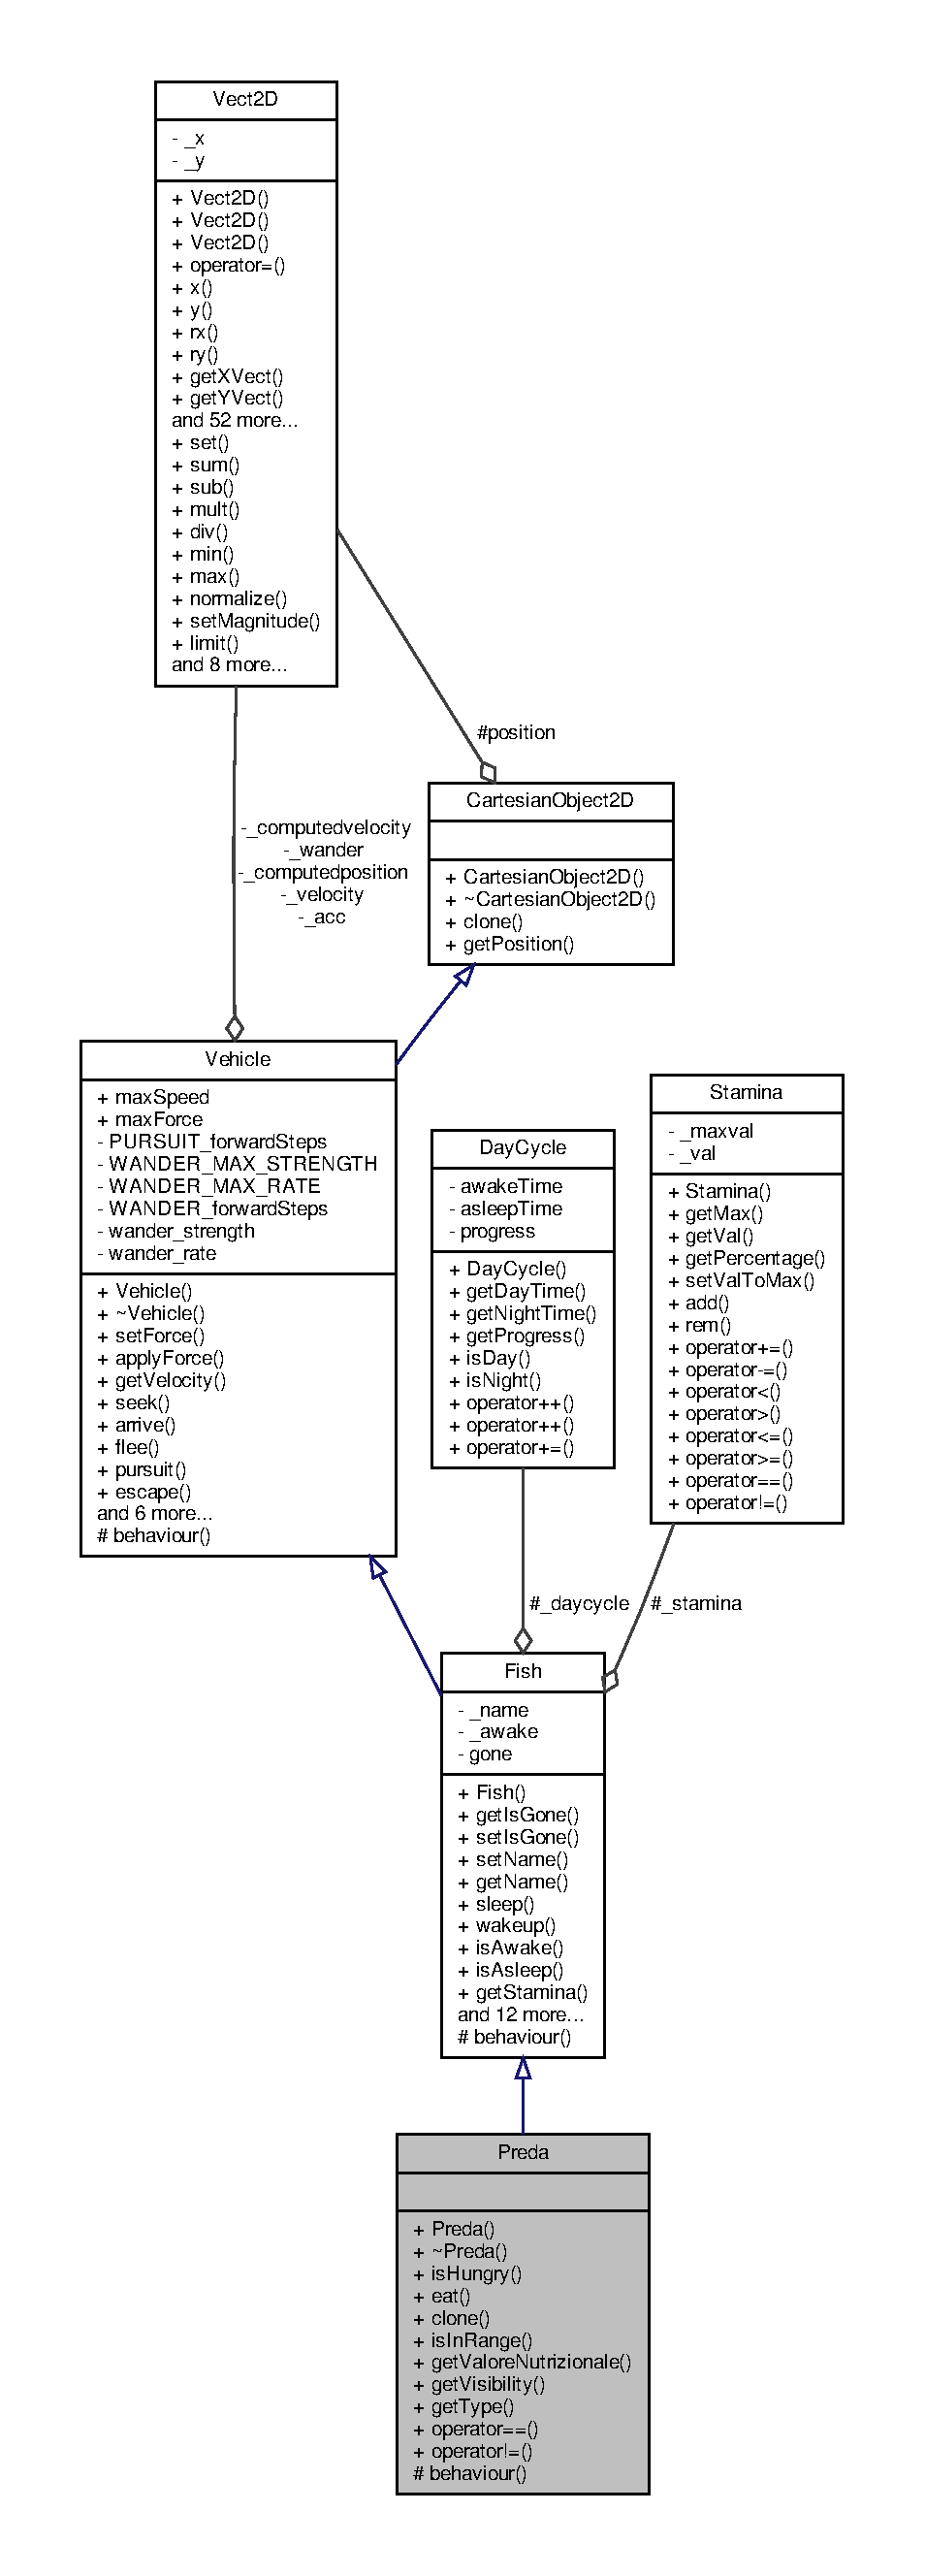
\includegraphics[height=550pt]{classPreda__coll__graph}
\end{center}
\end{figure}
\subsection*{Public Member Functions}
\begin{DoxyCompactItemize}
\item 
\hyperlink{classPreda_aeddef5ec6e57cc15875046523d8ed119_aeddef5ec6e57cc15875046523d8ed119}{Preda} (const \hyperlink{classVect2D}{Vect2D} \&, const std\+::string \&)
\item 
virtual \hyperlink{classPreda_ab33b836828f2273af29692406d985a8b_ab33b836828f2273af29692406d985a8b}{$\sim$\+Preda} ()
\item 
virtual bool \hyperlink{classPreda_ae63bc07a928fe4b6685fcdd06c22a506_ae63bc07a928fe4b6685fcdd06c22a506}{is\+Hungry} () const override
\item 
virtual void \hyperlink{classPreda_ac7d83956cf08c9300d331a5505ab3118_ac7d83956cf08c9300d331a5505ab3118}{eat} (\hyperlink{classFish}{Fish} \&) override
\item 
virtual \hyperlink{classPreda}{Preda} $\ast$ \hyperlink{classPreda_a12baf94e52873bf3b9a9a9da84c357c5_a12baf94e52873bf3b9a9a9da84c357c5}{clone} () const override
\item 
virtual bool \hyperlink{classPreda_a4014c320e53abbfc7cbfb30f18791db2_a4014c320e53abbfc7cbfb30f18791db2}{is\+In\+Range} (const \hyperlink{classVect2D}{Vect2D} \&) const override
\item 
virtual int \hyperlink{classPreda_a9f0e2e1f347466a5084f887dab6c218f_a9f0e2e1f347466a5084f887dab6c218f}{get\+Valore\+Nutrizionale} () const override
\item 
virtual double \hyperlink{classPreda_a0541a146d9779d0391c0cff244964dd4_a0541a146d9779d0391c0cff244964dd4}{get\+Visibility} () const override
\item 
virtual std\+::string \hyperlink{classPreda_a0acc2147813c125f3fdd7b0743d62b81_a0acc2147813c125f3fdd7b0743d62b81}{get\+Type} () const override
\item 
virtual bool \hyperlink{classPreda_a38ba49e7ab329e8ebbf23f242d3dd084_a38ba49e7ab329e8ebbf23f242d3dd084}{operator==} (const \hyperlink{classFish}{Fish} \&) const override
\item 
virtual bool \hyperlink{classPreda_a69a59a55918bddb47457275763b2b352_a69a59a55918bddb47457275763b2b352}{operator!=} (const \hyperlink{classFish}{Fish} \&) const override
\item 
bool \hyperlink{classFish_a64e050916c0094ac377b8ec0d86a000b_a64e050916c0094ac377b8ec0d86a000b}{get\+Is\+Gone} () const
\item 
void \hyperlink{classFish_ad7d3a39831fa4a170a63dde98474b728_ad7d3a39831fa4a170a63dde98474b728}{set\+Is\+Gone} ()
\item 
void \hyperlink{classFish_a27a489adca6d1dc91b011ee97f36ae75_a27a489adca6d1dc91b011ee97f36ae75}{set\+Name} (const std\+::string \&)
\item 
const std\+::string \& \hyperlink{classFish_a96583314997aab0826f1c595f7d58938_a96583314997aab0826f1c595f7d58938}{get\+Name} () const
\item 
void \hyperlink{classFish_acac2f4f6c31adfb0c8f4eb78853445bb_acac2f4f6c31adfb0c8f4eb78853445bb}{sleep} ()
\item 
void \hyperlink{classFish_a8160593a43c6ce5263c6280e0cf0a7be_a8160593a43c6ce5263c6280e0cf0a7be}{wakeup} ()
\item 
bool \hyperlink{classFish_aea2a66c3cd46d3a672c82ca9e537b9ec_aea2a66c3cd46d3a672c82ca9e537b9ec}{is\+Awake} () const
\item 
bool \hyperlink{classFish_a4772391eb9a92dca61b810b40705709b_a4772391eb9a92dca61b810b40705709b}{is\+Asleep} () const
\item 
const \hyperlink{classStamina}{Stamina} \& \hyperlink{classFish_a8637a567ecb17376bed45783d5ddb53d_a8637a567ecb17376bed45783d5ddb53d}{get\+Stamina} () const
\item 
virtual bool \hyperlink{classFish_a9a94edb09498e8d0d2381c2cc3e2e9dc_a9a94edb09498e8d0d2381c2cc3e2e9dc}{can\+Sleep} () const
\item 
virtual bool \hyperlink{classFish_a033298bf0dc885b82dbd195fc4997643_a033298bf0dc885b82dbd195fc4997643}{can\+Wakeup} () const
\item 
void \hyperlink{classVehicle_a03e22c522e6f526f95428c81d0762833_a03e22c522e6f526f95428c81d0762833}{set\+Force} (const \hyperlink{classVect2D}{Vect2D} \&)
\item 
void \hyperlink{classVehicle_a82fbbd5aafc1ba89c3daa4da09989bbe_a82fbbd5aafc1ba89c3daa4da09989bbe}{apply\+Force} (const \hyperlink{classVect2D}{Vect2D} \&, const double \&=1)
\item 
const \hyperlink{classVect2D}{Vect2D} \& \hyperlink{classVehicle_a87b8266cb3495e8444233a0724e1bf07_a87b8266cb3495e8444233a0724e1bf07}{get\+Velocity} () const
\item 
\hyperlink{classVect2D}{Vect2D} \hyperlink{classVehicle_a86c0b5ddcf64443bc090657cd29832bf_a86c0b5ddcf64443bc090657cd29832bf}{seek} (const \hyperlink{classVect2D}{Vect2D} \&) const
\item 
\hyperlink{classVect2D}{Vect2D} \hyperlink{classVehicle_a55f8bb6cfbdd97219c2cea6cf3ad3826_a55f8bb6cfbdd97219c2cea6cf3ad3826}{arrive} (const \hyperlink{classVect2D}{Vect2D} \&) const
\item 
\hyperlink{classVect2D}{Vect2D} \hyperlink{classVehicle_ac7dbbb2942b8d642b2ab071def1c2fdb_ac7dbbb2942b8d642b2ab071def1c2fdb}{flee} (const \hyperlink{classVect2D}{Vect2D} \&) const
\item 
\hyperlink{classVect2D}{Vect2D} \hyperlink{classVehicle_a9dd4f4a06b4abd3324d317c27bb867d2_a9dd4f4a06b4abd3324d317c27bb867d2}{pursuit} (const \hyperlink{classVehicle}{Vehicle} \&) const
\item 
\hyperlink{classVect2D}{Vect2D} \hyperlink{classVehicle_ae5fbf395cbebf51498cbe8b2baaddc16_ae5fbf395cbebf51498cbe8b2baaddc16}{escape} (const \hyperlink{classVehicle}{Vehicle} \&) const
\item 
\hyperlink{classVect2D}{Vect2D} \hyperlink{classVehicle_af9da94116706c94e5f26df42c258dc6e_af9da94116706c94e5f26df42c258dc6e}{wander} ()
\item 
\hyperlink{classVect2D}{Vect2D} \hyperlink{classVehicle_a9a1cb1e5dab4a474fbe0c1c49482d0ee_a9a1cb1e5dab4a474fbe0c1c49482d0ee}{stop} () const
\item 
\hyperlink{classVect2D}{Vect2D} \hyperlink{classVehicle_a6149abf3e3f67df45d950562034d0fae_a6149abf3e3f67df45d950562034d0fae}{stay\+Within\+Borders} (const \hyperlink{classVect2D}{Vect2D} \&, const unsigned int distance) const
\item 
virtual void \hyperlink{classVehicle_aa4ffd7e5fd11297950347de4e8b5ec93_aa4ffd7e5fd11297950347de4e8b5ec93}{advance} (\hyperlink{classAquarius}{Aquarius} $\ast$a, int phase) final
\item 
\hyperlink{classVect2D}{Vect2D} \hyperlink{classCartesianObject2D_aa3a6b63777852ab9eb9408ed2536abe2_aa3a6b63777852ab9eb9408ed2536abe2}{get\+Position} () const
\end{DoxyCompactItemize}
\subsection*{Static Public Attributes}
\begin{DoxyCompactItemize}
\item 
static const double \hyperlink{classVehicle_aab47c62e89baa5b7e52c2292451fbcb6_aab47c62e89baa5b7e52c2292451fbcb6}{max\+Speed} = 5
\item 
static const double \hyperlink{classVehicle_a95c56790e3dc52ab0fa54c279920be54_a95c56790e3dc52ab0fa54c279920be54}{max\+Force} = .\+15
\end{DoxyCompactItemize}
\subsection*{Protected Member Functions}
\begin{DoxyCompactItemize}
\item 
virtual void \hyperlink{classPreda_a5c0724c3854a2fff92f3c2308514c89e_a5c0724c3854a2fff92f3c2308514c89e}{behaviour} (\hyperlink{classAquarius}{Aquarius} $\ast$) override
\end{DoxyCompactItemize}
\subsection*{Protected Attributes}
\begin{DoxyCompactItemize}
\item 
\hyperlink{classDayCycle}{Day\+Cycle} \hyperlink{classFish_a4b8a32e2a5165ddd1f8af27f4346b3eb_a4b8a32e2a5165ddd1f8af27f4346b3eb}{\+\_\+daycycle}
\item 
\hyperlink{classStamina}{Stamina} \hyperlink{classFish_a4948331d0f556344bda8314828eec8dd_a4948331d0f556344bda8314828eec8dd}{\+\_\+stamina}
\item 
\hyperlink{classVect2D}{Vect2D} \hyperlink{classCartesianObject2D_ae02ec6ed11f9bfc0c748da033d6a32f9_ae02ec6ed11f9bfc0c748da033d6a32f9}{position}
\end{DoxyCompactItemize}


\subsection{Constructor \& Destructor Documentation}
\mbox{\Hypertarget{classPreda_aeddef5ec6e57cc15875046523d8ed119_aeddef5ec6e57cc15875046523d8ed119}\label{classPreda_aeddef5ec6e57cc15875046523d8ed119_aeddef5ec6e57cc15875046523d8ed119}} 
\index{Preda@{Preda}!Preda@{Preda}}
\index{Preda@{Preda}!Preda@{Preda}}
\subsubsection{\texorpdfstring{Preda()}{Preda()}}
{\footnotesize\ttfamily Preda\+::\+Preda (\begin{DoxyParamCaption}\item[{const \hyperlink{classVect2D}{Vect2D} \&}]{position,  }\item[{const std\+::string \&}]{name }\end{DoxyParamCaption})}

\mbox{\Hypertarget{classPreda_ab33b836828f2273af29692406d985a8b_ab33b836828f2273af29692406d985a8b}\label{classPreda_ab33b836828f2273af29692406d985a8b_ab33b836828f2273af29692406d985a8b}} 
\index{Preda@{Preda}!````~Preda@{$\sim$\+Preda}}
\index{````~Preda@{$\sim$\+Preda}!Preda@{Preda}}
\subsubsection{\texorpdfstring{$\sim$\+Preda()}{~Preda()}}
{\footnotesize\ttfamily Preda\+::$\sim$\+Preda (\begin{DoxyParamCaption}{ }\end{DoxyParamCaption})\hspace{0.3cm}{\ttfamily [virtual]}}



\subsection{Member Function Documentation}
\mbox{\Hypertarget{classVehicle_aa4ffd7e5fd11297950347de4e8b5ec93_aa4ffd7e5fd11297950347de4e8b5ec93}\label{classVehicle_aa4ffd7e5fd11297950347de4e8b5ec93_aa4ffd7e5fd11297950347de4e8b5ec93}} 
\index{Preda@{Preda}!advance@{advance}}
\index{advance@{advance}!Preda@{Preda}}
\subsubsection{\texorpdfstring{advance()}{advance()}}
{\footnotesize\ttfamily void Vehicle\+::advance (\begin{DoxyParamCaption}\item[{\hyperlink{classAquarius}{Aquarius} $\ast$}]{a,  }\item[{int}]{phase }\end{DoxyParamCaption})\hspace{0.3cm}{\ttfamily [final]}, {\ttfamily [virtual]}, {\ttfamily [inherited]}}

\mbox{\Hypertarget{classVehicle_a82fbbd5aafc1ba89c3daa4da09989bbe_a82fbbd5aafc1ba89c3daa4da09989bbe}\label{classVehicle_a82fbbd5aafc1ba89c3daa4da09989bbe_a82fbbd5aafc1ba89c3daa4da09989bbe}} 
\index{Preda@{Preda}!apply\+Force@{apply\+Force}}
\index{apply\+Force@{apply\+Force}!Preda@{Preda}}
\subsubsection{\texorpdfstring{apply\+Force()}{applyForce()}}
{\footnotesize\ttfamily void Vehicle\+::apply\+Force (\begin{DoxyParamCaption}\item[{const \hyperlink{classVect2D}{Vect2D} \&}]{acc,  }\item[{const double \&}]{weight = {\ttfamily 1} }\end{DoxyParamCaption})\hspace{0.3cm}{\ttfamily [inherited]}}

Add the force of acceleration, to the already calculated one 
\begin{DoxyParams}{Parameters}
{\em acc} & \\
\hline
{\em weight} & \\
\hline
\end{DoxyParams}
\mbox{\Hypertarget{classVehicle_a55f8bb6cfbdd97219c2cea6cf3ad3826_a55f8bb6cfbdd97219c2cea6cf3ad3826}\label{classVehicle_a55f8bb6cfbdd97219c2cea6cf3ad3826_a55f8bb6cfbdd97219c2cea6cf3ad3826}} 
\index{Preda@{Preda}!arrive@{arrive}}
\index{arrive@{arrive}!Preda@{Preda}}
\subsubsection{\texorpdfstring{arrive()}{arrive()}}
{\footnotesize\ttfamily \hyperlink{classVect2D}{Vect2D} Vehicle\+::arrive (\begin{DoxyParamCaption}\item[{const \hyperlink{classVect2D}{Vect2D} \&}]{target }\end{DoxyParamCaption}) const\hspace{0.3cm}{\ttfamily [inherited]}}

\mbox{\Hypertarget{classPreda_a5c0724c3854a2fff92f3c2308514c89e_a5c0724c3854a2fff92f3c2308514c89e}\label{classPreda_a5c0724c3854a2fff92f3c2308514c89e_a5c0724c3854a2fff92f3c2308514c89e}} 
\index{Preda@{Preda}!behaviour@{behaviour}}
\index{behaviour@{behaviour}!Preda@{Preda}}
\subsubsection{\texorpdfstring{behaviour()}{behaviour()}}
{\footnotesize\ttfamily void Preda\+::behaviour (\begin{DoxyParamCaption}\item[{\hyperlink{classAquarius}{Aquarius} $\ast$}]{ }\end{DoxyParamCaption})\hspace{0.3cm}{\ttfamily [override]}, {\ttfamily [protected]}, {\ttfamily [virtual]}}

Calculates the behaviour of the vehicle 
\begin{DoxyParams}{Parameters}
{\em Aquarius$\ast$} & aquarius pointer \\
\hline
\end{DoxyParams}
\begin{DoxyReturn}{Returns}
\hyperlink{classVect2D}{Vect2D} the acceleration 
\end{DoxyReturn}


Reimplemented from \hyperlink{classFish_abffd423bc7a7730aafa80ec9c0cec9a0_abffd423bc7a7730aafa80ec9c0cec9a0}{Fish}.

\mbox{\Hypertarget{classFish_a9a94edb09498e8d0d2381c2cc3e2e9dc_a9a94edb09498e8d0d2381c2cc3e2e9dc}\label{classFish_a9a94edb09498e8d0d2381c2cc3e2e9dc_a9a94edb09498e8d0d2381c2cc3e2e9dc}} 
\index{Preda@{Preda}!can\+Sleep@{can\+Sleep}}
\index{can\+Sleep@{can\+Sleep}!Preda@{Preda}}
\subsubsection{\texorpdfstring{can\+Sleep()}{canSleep()}}
{\footnotesize\ttfamily bool Fish\+::can\+Sleep (\begin{DoxyParamCaption}{ }\end{DoxyParamCaption}) const\hspace{0.3cm}{\ttfamily [virtual]}, {\ttfamily [inherited]}}

\mbox{\Hypertarget{classFish_a033298bf0dc885b82dbd195fc4997643_a033298bf0dc885b82dbd195fc4997643}\label{classFish_a033298bf0dc885b82dbd195fc4997643_a033298bf0dc885b82dbd195fc4997643}} 
\index{Preda@{Preda}!can\+Wakeup@{can\+Wakeup}}
\index{can\+Wakeup@{can\+Wakeup}!Preda@{Preda}}
\subsubsection{\texorpdfstring{can\+Wakeup()}{canWakeup()}}
{\footnotesize\ttfamily bool Fish\+::can\+Wakeup (\begin{DoxyParamCaption}{ }\end{DoxyParamCaption}) const\hspace{0.3cm}{\ttfamily [virtual]}, {\ttfamily [inherited]}}

\mbox{\Hypertarget{classPreda_a12baf94e52873bf3b9a9a9da84c357c5_a12baf94e52873bf3b9a9a9da84c357c5}\label{classPreda_a12baf94e52873bf3b9a9a9da84c357c5_a12baf94e52873bf3b9a9a9da84c357c5}} 
\index{Preda@{Preda}!clone@{clone}}
\index{clone@{clone}!Preda@{Preda}}
\subsubsection{\texorpdfstring{clone()}{clone()}}
{\footnotesize\ttfamily \hyperlink{classPreda}{Preda} $\ast$ Preda\+::clone (\begin{DoxyParamCaption}{ }\end{DoxyParamCaption}) const\hspace{0.3cm}{\ttfamily [override]}, {\ttfamily [virtual]}}



Implements \hyperlink{classFish_a6732945f7373a28b1723e55de8a65e13_a6732945f7373a28b1723e55de8a65e13}{Fish}.

\mbox{\Hypertarget{classPreda_ac7d83956cf08c9300d331a5505ab3118_ac7d83956cf08c9300d331a5505ab3118}\label{classPreda_ac7d83956cf08c9300d331a5505ab3118_ac7d83956cf08c9300d331a5505ab3118}} 
\index{Preda@{Preda}!eat@{eat}}
\index{eat@{eat}!Preda@{Preda}}
\subsubsection{\texorpdfstring{eat()}{eat()}}
{\footnotesize\ttfamily void Preda\+::eat (\begin{DoxyParamCaption}\item[{\hyperlink{classFish}{Fish} \&}]{ }\end{DoxyParamCaption})\hspace{0.3cm}{\ttfamily [override]}, {\ttfamily [virtual]}}



Implements \hyperlink{classFish_ae551e094ddda73e896de484dcb460412_ae551e094ddda73e896de484dcb460412}{Fish}.

\mbox{\Hypertarget{classVehicle_ae5fbf395cbebf51498cbe8b2baaddc16_ae5fbf395cbebf51498cbe8b2baaddc16}\label{classVehicle_ae5fbf395cbebf51498cbe8b2baaddc16_ae5fbf395cbebf51498cbe8b2baaddc16}} 
\index{Preda@{Preda}!escape@{escape}}
\index{escape@{escape}!Preda@{Preda}}
\subsubsection{\texorpdfstring{escape()}{escape()}}
{\footnotesize\ttfamily \hyperlink{classVect2D}{Vect2D} Vehicle\+::escape (\begin{DoxyParamCaption}\item[{const \hyperlink{classVehicle}{Vehicle} \&}]{v }\end{DoxyParamCaption}) const\hspace{0.3cm}{\ttfamily [inherited]}}

\mbox{\Hypertarget{classVehicle_ac7dbbb2942b8d642b2ab071def1c2fdb_ac7dbbb2942b8d642b2ab071def1c2fdb}\label{classVehicle_ac7dbbb2942b8d642b2ab071def1c2fdb_ac7dbbb2942b8d642b2ab071def1c2fdb}} 
\index{Preda@{Preda}!flee@{flee}}
\index{flee@{flee}!Preda@{Preda}}
\subsubsection{\texorpdfstring{flee()}{flee()}}
{\footnotesize\ttfamily \hyperlink{classVect2D}{Vect2D} Vehicle\+::flee (\begin{DoxyParamCaption}\item[{const \hyperlink{classVect2D}{Vect2D} \&}]{target }\end{DoxyParamCaption}) const\hspace{0.3cm}{\ttfamily [inherited]}}

\mbox{\Hypertarget{classFish_a64e050916c0094ac377b8ec0d86a000b_a64e050916c0094ac377b8ec0d86a000b}\label{classFish_a64e050916c0094ac377b8ec0d86a000b_a64e050916c0094ac377b8ec0d86a000b}} 
\index{Preda@{Preda}!get\+Is\+Gone@{get\+Is\+Gone}}
\index{get\+Is\+Gone@{get\+Is\+Gone}!Preda@{Preda}}
\subsubsection{\texorpdfstring{get\+Is\+Gone()}{getIsGone()}}
{\footnotesize\ttfamily bool Fish\+::get\+Is\+Gone (\begin{DoxyParamCaption}{ }\end{DoxyParamCaption}) const\hspace{0.3cm}{\ttfamily [inherited]}}

\mbox{\Hypertarget{classFish_a96583314997aab0826f1c595f7d58938_a96583314997aab0826f1c595f7d58938}\label{classFish_a96583314997aab0826f1c595f7d58938_a96583314997aab0826f1c595f7d58938}} 
\index{Preda@{Preda}!get\+Name@{get\+Name}}
\index{get\+Name@{get\+Name}!Preda@{Preda}}
\subsubsection{\texorpdfstring{get\+Name()}{getName()}}
{\footnotesize\ttfamily const std\+::string \& Fish\+::get\+Name (\begin{DoxyParamCaption}{ }\end{DoxyParamCaption}) const\hspace{0.3cm}{\ttfamily [inherited]}}

\mbox{\Hypertarget{classCartesianObject2D_aa3a6b63777852ab9eb9408ed2536abe2_aa3a6b63777852ab9eb9408ed2536abe2}\label{classCartesianObject2D_aa3a6b63777852ab9eb9408ed2536abe2_aa3a6b63777852ab9eb9408ed2536abe2}} 
\index{Preda@{Preda}!get\+Position@{get\+Position}}
\index{get\+Position@{get\+Position}!Preda@{Preda}}
\subsubsection{\texorpdfstring{get\+Position()}{getPosition()}}
{\footnotesize\ttfamily \hyperlink{classVect2D}{Vect2D} Cartesian\+Object2\+D\+::get\+Position (\begin{DoxyParamCaption}{ }\end{DoxyParamCaption}) const\hspace{0.3cm}{\ttfamily [inherited]}}

\mbox{\Hypertarget{classFish_a8637a567ecb17376bed45783d5ddb53d_a8637a567ecb17376bed45783d5ddb53d}\label{classFish_a8637a567ecb17376bed45783d5ddb53d_a8637a567ecb17376bed45783d5ddb53d}} 
\index{Preda@{Preda}!get\+Stamina@{get\+Stamina}}
\index{get\+Stamina@{get\+Stamina}!Preda@{Preda}}
\subsubsection{\texorpdfstring{get\+Stamina()}{getStamina()}}
{\footnotesize\ttfamily const \hyperlink{classStamina}{Stamina} \& Fish\+::get\+Stamina (\begin{DoxyParamCaption}{ }\end{DoxyParamCaption}) const\hspace{0.3cm}{\ttfamily [inherited]}}

\mbox{\Hypertarget{classPreda_a0acc2147813c125f3fdd7b0743d62b81_a0acc2147813c125f3fdd7b0743d62b81}\label{classPreda_a0acc2147813c125f3fdd7b0743d62b81_a0acc2147813c125f3fdd7b0743d62b81}} 
\index{Preda@{Preda}!get\+Type@{get\+Type}}
\index{get\+Type@{get\+Type}!Preda@{Preda}}
\subsubsection{\texorpdfstring{get\+Type()}{getType()}}
{\footnotesize\ttfamily std\+::string Preda\+::get\+Type (\begin{DoxyParamCaption}{ }\end{DoxyParamCaption}) const\hspace{0.3cm}{\ttfamily [override]}, {\ttfamily [virtual]}}



Implements \hyperlink{classFish_adb00fb6bac2fad27660107c12d1a7fa2_adb00fb6bac2fad27660107c12d1a7fa2}{Fish}.

\mbox{\Hypertarget{classPreda_a9f0e2e1f347466a5084f887dab6c218f_a9f0e2e1f347466a5084f887dab6c218f}\label{classPreda_a9f0e2e1f347466a5084f887dab6c218f_a9f0e2e1f347466a5084f887dab6c218f}} 
\index{Preda@{Preda}!get\+Valore\+Nutrizionale@{get\+Valore\+Nutrizionale}}
\index{get\+Valore\+Nutrizionale@{get\+Valore\+Nutrizionale}!Preda@{Preda}}
\subsubsection{\texorpdfstring{get\+Valore\+Nutrizionale()}{getValoreNutrizionale()}}
{\footnotesize\ttfamily int Preda\+::get\+Valore\+Nutrizionale (\begin{DoxyParamCaption}{ }\end{DoxyParamCaption}) const\hspace{0.3cm}{\ttfamily [override]}, {\ttfamily [virtual]}}



Implements \hyperlink{classFish_a97dd71f31af1e36a630944c5c5b8ff33_a97dd71f31af1e36a630944c5c5b8ff33}{Fish}.

\mbox{\Hypertarget{classVehicle_a87b8266cb3495e8444233a0724e1bf07_a87b8266cb3495e8444233a0724e1bf07}\label{classVehicle_a87b8266cb3495e8444233a0724e1bf07_a87b8266cb3495e8444233a0724e1bf07}} 
\index{Preda@{Preda}!get\+Velocity@{get\+Velocity}}
\index{get\+Velocity@{get\+Velocity}!Preda@{Preda}}
\subsubsection{\texorpdfstring{get\+Velocity()}{getVelocity()}}
{\footnotesize\ttfamily const \hyperlink{classVect2D}{Vect2D} \& Vehicle\+::get\+Velocity (\begin{DoxyParamCaption}{ }\end{DoxyParamCaption}) const\hspace{0.3cm}{\ttfamily [inherited]}}

\mbox{\Hypertarget{classPreda_a0541a146d9779d0391c0cff244964dd4_a0541a146d9779d0391c0cff244964dd4}\label{classPreda_a0541a146d9779d0391c0cff244964dd4_a0541a146d9779d0391c0cff244964dd4}} 
\index{Preda@{Preda}!get\+Visibility@{get\+Visibility}}
\index{get\+Visibility@{get\+Visibility}!Preda@{Preda}}
\subsubsection{\texorpdfstring{get\+Visibility()}{getVisibility()}}
{\footnotesize\ttfamily double Preda\+::get\+Visibility (\begin{DoxyParamCaption}{ }\end{DoxyParamCaption}) const\hspace{0.3cm}{\ttfamily [override]}, {\ttfamily [virtual]}}



Implements \hyperlink{classFish_a6c20ea483d1f6237ebf01aee3f2b6e88_a6c20ea483d1f6237ebf01aee3f2b6e88}{Fish}.

\mbox{\Hypertarget{classFish_a4772391eb9a92dca61b810b40705709b_a4772391eb9a92dca61b810b40705709b}\label{classFish_a4772391eb9a92dca61b810b40705709b_a4772391eb9a92dca61b810b40705709b}} 
\index{Preda@{Preda}!is\+Asleep@{is\+Asleep}}
\index{is\+Asleep@{is\+Asleep}!Preda@{Preda}}
\subsubsection{\texorpdfstring{is\+Asleep()}{isAsleep()}}
{\footnotesize\ttfamily bool Fish\+::is\+Asleep (\begin{DoxyParamCaption}{ }\end{DoxyParamCaption}) const\hspace{0.3cm}{\ttfamily [inherited]}}

\mbox{\Hypertarget{classFish_aea2a66c3cd46d3a672c82ca9e537b9ec_aea2a66c3cd46d3a672c82ca9e537b9ec}\label{classFish_aea2a66c3cd46d3a672c82ca9e537b9ec_aea2a66c3cd46d3a672c82ca9e537b9ec}} 
\index{Preda@{Preda}!is\+Awake@{is\+Awake}}
\index{is\+Awake@{is\+Awake}!Preda@{Preda}}
\subsubsection{\texorpdfstring{is\+Awake()}{isAwake()}}
{\footnotesize\ttfamily bool Fish\+::is\+Awake (\begin{DoxyParamCaption}{ }\end{DoxyParamCaption}) const\hspace{0.3cm}{\ttfamily [inherited]}}

\mbox{\Hypertarget{classPreda_ae63bc07a928fe4b6685fcdd06c22a506_ae63bc07a928fe4b6685fcdd06c22a506}\label{classPreda_ae63bc07a928fe4b6685fcdd06c22a506_ae63bc07a928fe4b6685fcdd06c22a506}} 
\index{Preda@{Preda}!is\+Hungry@{is\+Hungry}}
\index{is\+Hungry@{is\+Hungry}!Preda@{Preda}}
\subsubsection{\texorpdfstring{is\+Hungry()}{isHungry()}}
{\footnotesize\ttfamily bool Preda\+::is\+Hungry (\begin{DoxyParamCaption}{ }\end{DoxyParamCaption}) const\hspace{0.3cm}{\ttfamily [override]}, {\ttfamily [virtual]}}



Implements \hyperlink{classFish_a5fa8678bf28b723cfd2e225c217bb523_a5fa8678bf28b723cfd2e225c217bb523}{Fish}.

\mbox{\Hypertarget{classPreda_a4014c320e53abbfc7cbfb30f18791db2_a4014c320e53abbfc7cbfb30f18791db2}\label{classPreda_a4014c320e53abbfc7cbfb30f18791db2_a4014c320e53abbfc7cbfb30f18791db2}} 
\index{Preda@{Preda}!is\+In\+Range@{is\+In\+Range}}
\index{is\+In\+Range@{is\+In\+Range}!Preda@{Preda}}
\subsubsection{\texorpdfstring{is\+In\+Range()}{isInRange()}}
{\footnotesize\ttfamily bool Preda\+::is\+In\+Range (\begin{DoxyParamCaption}\item[{const \hyperlink{classVect2D}{Vect2D} \&}]{p }\end{DoxyParamCaption}) const\hspace{0.3cm}{\ttfamily [override]}, {\ttfamily [virtual]}}



Implements \hyperlink{classFish_a65e3b0bf5b211be6c4048aa5939331e1_a65e3b0bf5b211be6c4048aa5939331e1}{Fish}.

\mbox{\Hypertarget{classPreda_a69a59a55918bddb47457275763b2b352_a69a59a55918bddb47457275763b2b352}\label{classPreda_a69a59a55918bddb47457275763b2b352_a69a59a55918bddb47457275763b2b352}} 
\index{Preda@{Preda}!operator"!=@{operator"!=}}
\index{operator"!=@{operator"!=}!Preda@{Preda}}
\subsubsection{\texorpdfstring{operator"!=()}{operator!=()}}
{\footnotesize\ttfamily bool Preda\+::operator!= (\begin{DoxyParamCaption}\item[{const \hyperlink{classFish}{Fish} \&}]{f }\end{DoxyParamCaption}) const\hspace{0.3cm}{\ttfamily [override]}, {\ttfamily [virtual]}}



Implements \hyperlink{classFish_aa739aa5c06ff6054b051047bccd3bf6f_aa739aa5c06ff6054b051047bccd3bf6f}{Fish}.

\mbox{\Hypertarget{classPreda_a38ba49e7ab329e8ebbf23f242d3dd084_a38ba49e7ab329e8ebbf23f242d3dd084}\label{classPreda_a38ba49e7ab329e8ebbf23f242d3dd084_a38ba49e7ab329e8ebbf23f242d3dd084}} 
\index{Preda@{Preda}!operator==@{operator==}}
\index{operator==@{operator==}!Preda@{Preda}}
\subsubsection{\texorpdfstring{operator==()}{operator==()}}
{\footnotesize\ttfamily bool Preda\+::operator== (\begin{DoxyParamCaption}\item[{const \hyperlink{classFish}{Fish} \&}]{f }\end{DoxyParamCaption}) const\hspace{0.3cm}{\ttfamily [override]}, {\ttfamily [virtual]}}



Implements \hyperlink{classFish_a3abf96fe9cda276a4b3827464e2b0519_a3abf96fe9cda276a4b3827464e2b0519}{Fish}.

\mbox{\Hypertarget{classVehicle_a9dd4f4a06b4abd3324d317c27bb867d2_a9dd4f4a06b4abd3324d317c27bb867d2}\label{classVehicle_a9dd4f4a06b4abd3324d317c27bb867d2_a9dd4f4a06b4abd3324d317c27bb867d2}} 
\index{Preda@{Preda}!pursuit@{pursuit}}
\index{pursuit@{pursuit}!Preda@{Preda}}
\subsubsection{\texorpdfstring{pursuit()}{pursuit()}}
{\footnotesize\ttfamily \hyperlink{classVect2D}{Vect2D} Vehicle\+::pursuit (\begin{DoxyParamCaption}\item[{const \hyperlink{classVehicle}{Vehicle} \&}]{v }\end{DoxyParamCaption}) const\hspace{0.3cm}{\ttfamily [inherited]}}

\mbox{\Hypertarget{classVehicle_a86c0b5ddcf64443bc090657cd29832bf_a86c0b5ddcf64443bc090657cd29832bf}\label{classVehicle_a86c0b5ddcf64443bc090657cd29832bf_a86c0b5ddcf64443bc090657cd29832bf}} 
\index{Preda@{Preda}!seek@{seek}}
\index{seek@{seek}!Preda@{Preda}}
\subsubsection{\texorpdfstring{seek()}{seek()}}
{\footnotesize\ttfamily \hyperlink{classVect2D}{Vect2D} Vehicle\+::seek (\begin{DoxyParamCaption}\item[{const \hyperlink{classVect2D}{Vect2D} \&}]{target }\end{DoxyParamCaption}) const\hspace{0.3cm}{\ttfamily [inherited]}}

\mbox{\Hypertarget{classVehicle_a03e22c522e6f526f95428c81d0762833_a03e22c522e6f526f95428c81d0762833}\label{classVehicle_a03e22c522e6f526f95428c81d0762833_a03e22c522e6f526f95428c81d0762833}} 
\index{Preda@{Preda}!set\+Force@{set\+Force}}
\index{set\+Force@{set\+Force}!Preda@{Preda}}
\subsubsection{\texorpdfstring{set\+Force()}{setForce()}}
{\footnotesize\ttfamily void Vehicle\+::set\+Force (\begin{DoxyParamCaption}\item[{const \hyperlink{classVect2D}{Vect2D} \&}]{acc }\end{DoxyParamCaption})\hspace{0.3cm}{\ttfamily [inherited]}}

Set the force of acceleration 
\begin{DoxyParams}{Parameters}
{\em acc} & \\
\hline
\end{DoxyParams}
\mbox{\Hypertarget{classFish_ad7d3a39831fa4a170a63dde98474b728_ad7d3a39831fa4a170a63dde98474b728}\label{classFish_ad7d3a39831fa4a170a63dde98474b728_ad7d3a39831fa4a170a63dde98474b728}} 
\index{Preda@{Preda}!set\+Is\+Gone@{set\+Is\+Gone}}
\index{set\+Is\+Gone@{set\+Is\+Gone}!Preda@{Preda}}
\subsubsection{\texorpdfstring{set\+Is\+Gone()}{setIsGone()}}
{\footnotesize\ttfamily void Fish\+::set\+Is\+Gone (\begin{DoxyParamCaption}{ }\end{DoxyParamCaption})\hspace{0.3cm}{\ttfamily [inherited]}}

\mbox{\Hypertarget{classFish_a27a489adca6d1dc91b011ee97f36ae75_a27a489adca6d1dc91b011ee97f36ae75}\label{classFish_a27a489adca6d1dc91b011ee97f36ae75_a27a489adca6d1dc91b011ee97f36ae75}} 
\index{Preda@{Preda}!set\+Name@{set\+Name}}
\index{set\+Name@{set\+Name}!Preda@{Preda}}
\subsubsection{\texorpdfstring{set\+Name()}{setName()}}
{\footnotesize\ttfamily void Fish\+::set\+Name (\begin{DoxyParamCaption}\item[{const std\+::string \&}]{name }\end{DoxyParamCaption})\hspace{0.3cm}{\ttfamily [inherited]}}

\mbox{\Hypertarget{classFish_acac2f4f6c31adfb0c8f4eb78853445bb_acac2f4f6c31adfb0c8f4eb78853445bb}\label{classFish_acac2f4f6c31adfb0c8f4eb78853445bb_acac2f4f6c31adfb0c8f4eb78853445bb}} 
\index{Preda@{Preda}!sleep@{sleep}}
\index{sleep@{sleep}!Preda@{Preda}}
\subsubsection{\texorpdfstring{sleep()}{sleep()}}
{\footnotesize\ttfamily void Fish\+::sleep (\begin{DoxyParamCaption}{ }\end{DoxyParamCaption})\hspace{0.3cm}{\ttfamily [inherited]}}

\mbox{\Hypertarget{classVehicle_a6149abf3e3f67df45d950562034d0fae_a6149abf3e3f67df45d950562034d0fae}\label{classVehicle_a6149abf3e3f67df45d950562034d0fae_a6149abf3e3f67df45d950562034d0fae}} 
\index{Preda@{Preda}!stay\+Within\+Borders@{stay\+Within\+Borders}}
\index{stay\+Within\+Borders@{stay\+Within\+Borders}!Preda@{Preda}}
\subsubsection{\texorpdfstring{stay\+Within\+Borders()}{stayWithinBorders()}}
{\footnotesize\ttfamily \hyperlink{classVect2D}{Vect2D} Vehicle\+::stay\+Within\+Borders (\begin{DoxyParamCaption}\item[{const \hyperlink{classVect2D}{Vect2D} \&}]{size,  }\item[{const unsigned int}]{distance }\end{DoxyParamCaption}) const\hspace{0.3cm}{\ttfamily [inherited]}}

\mbox{\Hypertarget{classVehicle_a9a1cb1e5dab4a474fbe0c1c49482d0ee_a9a1cb1e5dab4a474fbe0c1c49482d0ee}\label{classVehicle_a9a1cb1e5dab4a474fbe0c1c49482d0ee_a9a1cb1e5dab4a474fbe0c1c49482d0ee}} 
\index{Preda@{Preda}!stop@{stop}}
\index{stop@{stop}!Preda@{Preda}}
\subsubsection{\texorpdfstring{stop()}{stop()}}
{\footnotesize\ttfamily \hyperlink{classVect2D}{Vect2D} Vehicle\+::stop (\begin{DoxyParamCaption}{ }\end{DoxyParamCaption}) const\hspace{0.3cm}{\ttfamily [inherited]}}

\mbox{\Hypertarget{classFish_a8160593a43c6ce5263c6280e0cf0a7be_a8160593a43c6ce5263c6280e0cf0a7be}\label{classFish_a8160593a43c6ce5263c6280e0cf0a7be_a8160593a43c6ce5263c6280e0cf0a7be}} 
\index{Preda@{Preda}!wakeup@{wakeup}}
\index{wakeup@{wakeup}!Preda@{Preda}}
\subsubsection{\texorpdfstring{wakeup()}{wakeup()}}
{\footnotesize\ttfamily void Fish\+::wakeup (\begin{DoxyParamCaption}{ }\end{DoxyParamCaption})\hspace{0.3cm}{\ttfamily [inherited]}}

\mbox{\Hypertarget{classVehicle_af9da94116706c94e5f26df42c258dc6e_af9da94116706c94e5f26df42c258dc6e}\label{classVehicle_af9da94116706c94e5f26df42c258dc6e_af9da94116706c94e5f26df42c258dc6e}} 
\index{Preda@{Preda}!wander@{wander}}
\index{wander@{wander}!Preda@{Preda}}
\subsubsection{\texorpdfstring{wander()}{wander()}}
{\footnotesize\ttfamily \hyperlink{classVect2D}{Vect2D} Vehicle\+::wander (\begin{DoxyParamCaption}{ }\end{DoxyParamCaption})\hspace{0.3cm}{\ttfamily [inherited]}}



\subsection{Member Data Documentation}
\mbox{\Hypertarget{classFish_a4b8a32e2a5165ddd1f8af27f4346b3eb_a4b8a32e2a5165ddd1f8af27f4346b3eb}\label{classFish_a4b8a32e2a5165ddd1f8af27f4346b3eb_a4b8a32e2a5165ddd1f8af27f4346b3eb}} 
\index{Preda@{Preda}!\+\_\+daycycle@{\+\_\+daycycle}}
\index{\+\_\+daycycle@{\+\_\+daycycle}!Preda@{Preda}}
\subsubsection{\texorpdfstring{\+\_\+daycycle}{\_daycycle}}
{\footnotesize\ttfamily \hyperlink{classDayCycle}{Day\+Cycle} Fish\+::\+\_\+daycycle\hspace{0.3cm}{\ttfamily [protected]}, {\ttfamily [inherited]}}

\mbox{\Hypertarget{classFish_a4948331d0f556344bda8314828eec8dd_a4948331d0f556344bda8314828eec8dd}\label{classFish_a4948331d0f556344bda8314828eec8dd_a4948331d0f556344bda8314828eec8dd}} 
\index{Preda@{Preda}!\+\_\+stamina@{\+\_\+stamina}}
\index{\+\_\+stamina@{\+\_\+stamina}!Preda@{Preda}}
\subsubsection{\texorpdfstring{\+\_\+stamina}{\_stamina}}
{\footnotesize\ttfamily \hyperlink{classStamina}{Stamina} Fish\+::\+\_\+stamina\hspace{0.3cm}{\ttfamily [protected]}, {\ttfamily [inherited]}}

\mbox{\Hypertarget{classVehicle_a95c56790e3dc52ab0fa54c279920be54_a95c56790e3dc52ab0fa54c279920be54}\label{classVehicle_a95c56790e3dc52ab0fa54c279920be54_a95c56790e3dc52ab0fa54c279920be54}} 
\index{Preda@{Preda}!max\+Force@{max\+Force}}
\index{max\+Force@{max\+Force}!Preda@{Preda}}
\subsubsection{\texorpdfstring{max\+Force}{maxForce}}
{\footnotesize\ttfamily const double Vehicle\+::max\+Force = .\+15\hspace{0.3cm}{\ttfamily [static]}, {\ttfamily [inherited]}}

\mbox{\Hypertarget{classVehicle_aab47c62e89baa5b7e52c2292451fbcb6_aab47c62e89baa5b7e52c2292451fbcb6}\label{classVehicle_aab47c62e89baa5b7e52c2292451fbcb6_aab47c62e89baa5b7e52c2292451fbcb6}} 
\index{Preda@{Preda}!max\+Speed@{max\+Speed}}
\index{max\+Speed@{max\+Speed}!Preda@{Preda}}
\subsubsection{\texorpdfstring{max\+Speed}{maxSpeed}}
{\footnotesize\ttfamily const double Vehicle\+::max\+Speed = 5\hspace{0.3cm}{\ttfamily [static]}, {\ttfamily [inherited]}}

\mbox{\Hypertarget{classCartesianObject2D_ae02ec6ed11f9bfc0c748da033d6a32f9_ae02ec6ed11f9bfc0c748da033d6a32f9}\label{classCartesianObject2D_ae02ec6ed11f9bfc0c748da033d6a32f9_ae02ec6ed11f9bfc0c748da033d6a32f9}} 
\index{Preda@{Preda}!position@{position}}
\index{position@{position}!Preda@{Preda}}
\subsubsection{\texorpdfstring{position}{position}}
{\footnotesize\ttfamily \hyperlink{classVect2D}{Vect2D} Cartesian\+Object2\+D\+::position\hspace{0.3cm}{\ttfamily [protected]}, {\ttfamily [inherited]}}



The documentation for this class was generated from the following files\+:\begin{DoxyCompactItemize}
\item 
include/\hyperlink{preda_8hpp}{preda.\+hpp}\item 
src/\hyperlink{preda_8cpp}{preda.\+cpp}\end{DoxyCompactItemize}

\hypertarget{classPredatore}{}\section{Predatore Class Reference}
\label{classPredatore}\index{Predatore@{Predatore}}


{\ttfamily \#include $<$predatore.\+hpp$>$}



Inheritance diagram for Predatore\+:\nopagebreak
\begin{figure}[H]
\begin{center}
\leavevmode
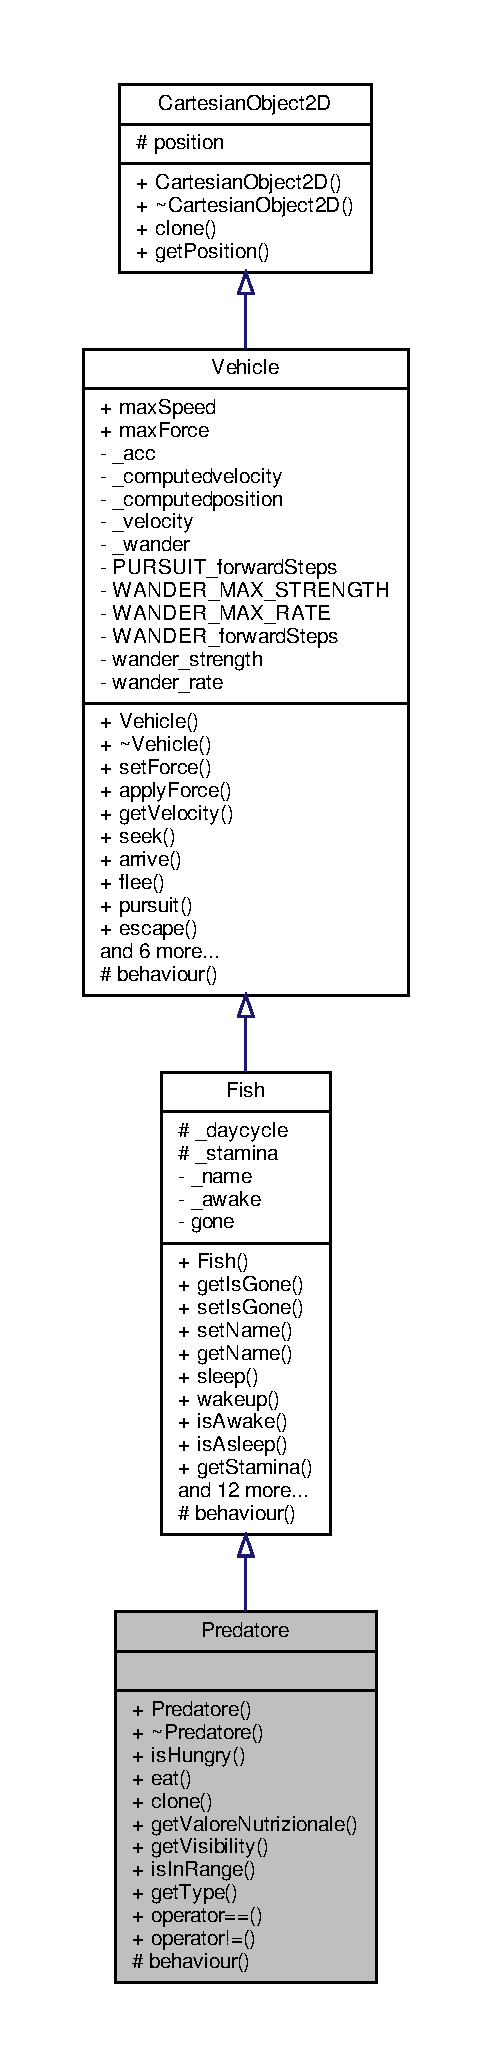
\includegraphics[height=550pt]{classPredatore__inherit__graph}
\end{center}
\end{figure}


Collaboration diagram for Predatore\+:\nopagebreak
\begin{figure}[H]
\begin{center}
\leavevmode
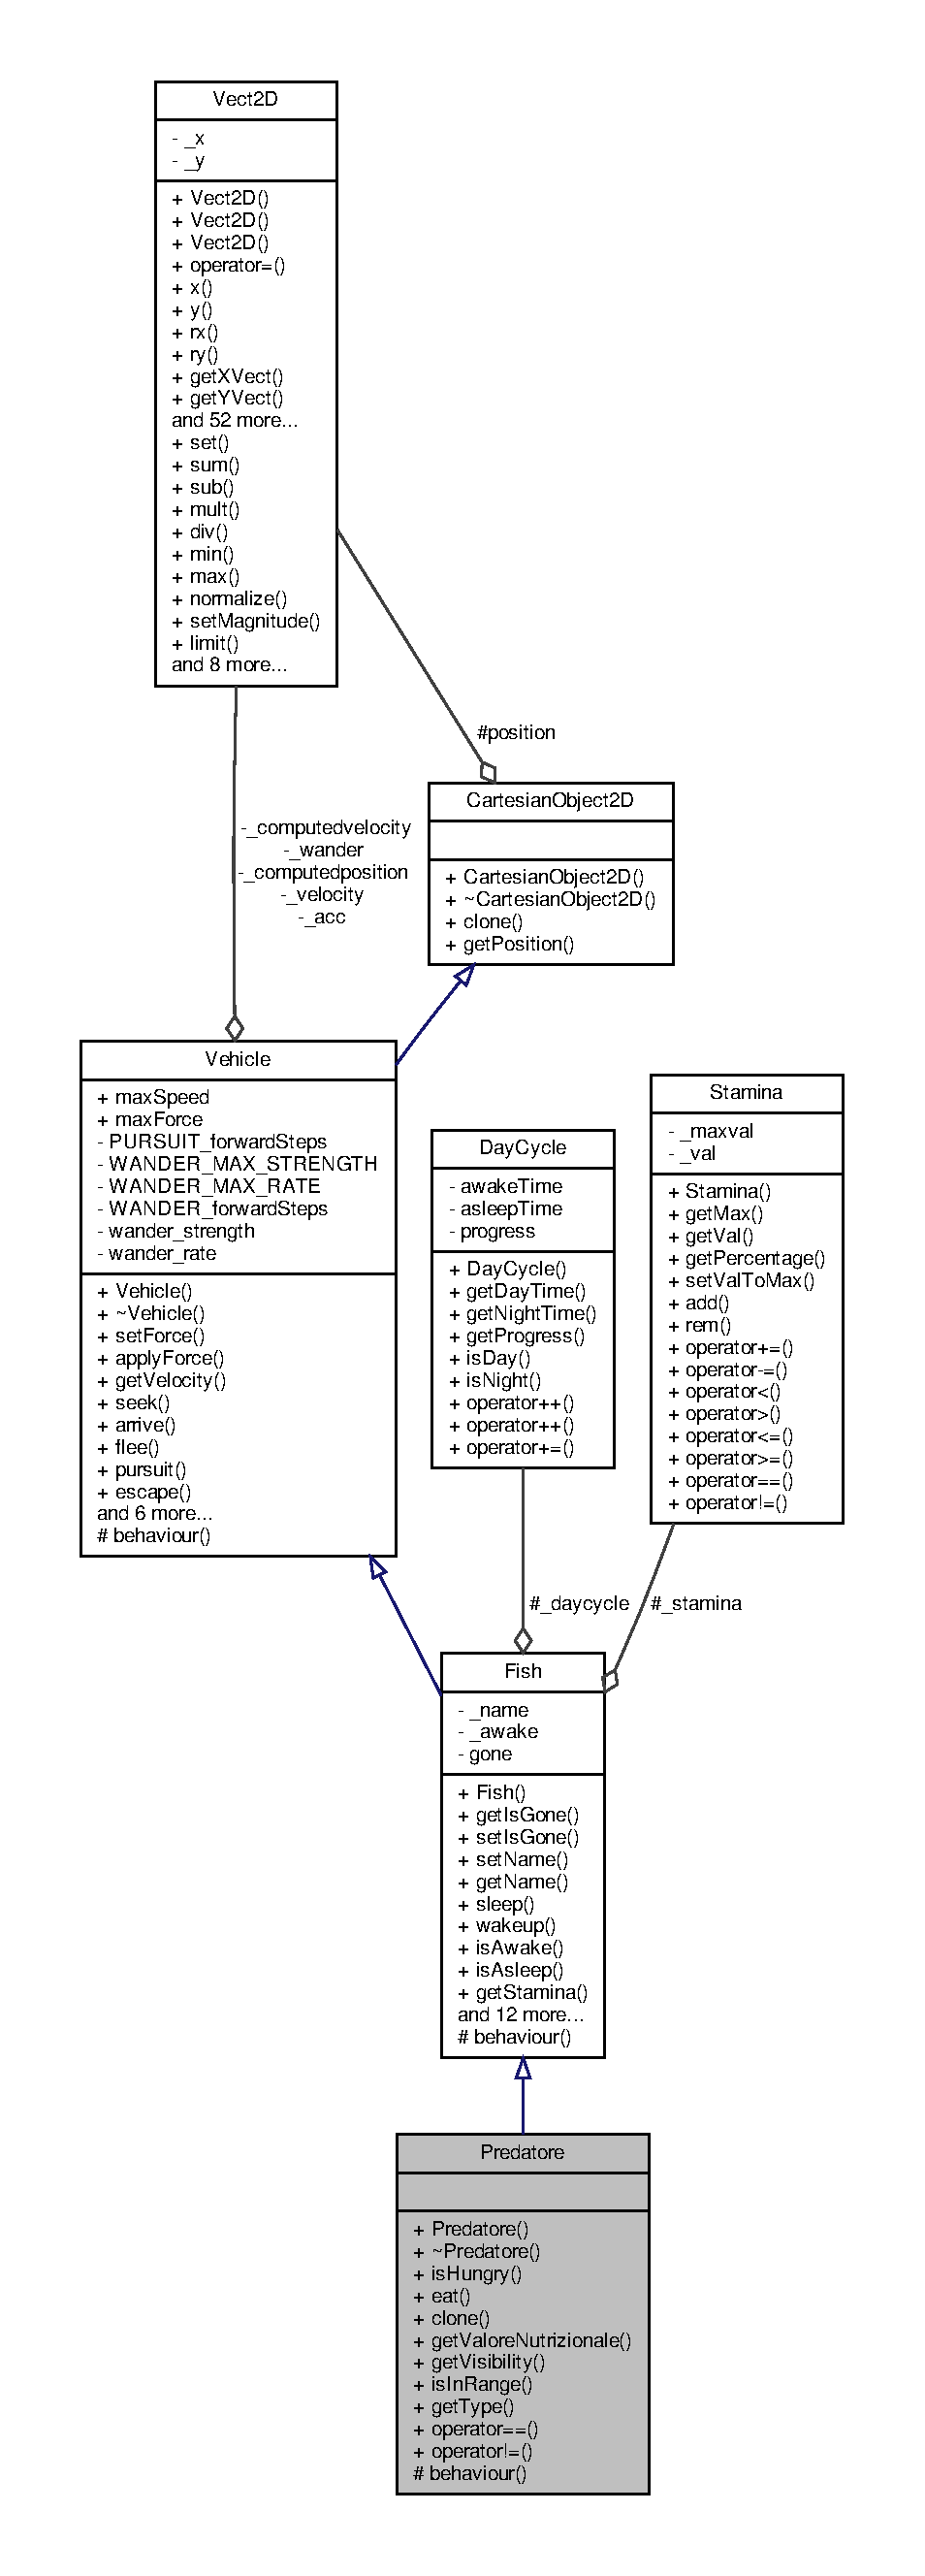
\includegraphics[height=550pt]{classPredatore__coll__graph}
\end{center}
\end{figure}
\subsection*{Public Member Functions}
\begin{DoxyCompactItemize}
\item 
\hyperlink{classPredatore_a8aa157df9ce0145ebd9211e867d27258_a8aa157df9ce0145ebd9211e867d27258}{Predatore} (const \hyperlink{classVect2D}{Vect2D} \&, const std\+::string \&=\char`\"{}no name\char`\"{})
\item 
virtual \hyperlink{classPredatore_a72b2c3e53a30cd50693cfeb7c4e838ca_a72b2c3e53a30cd50693cfeb7c4e838ca}{$\sim$\+Predatore} ()
\item 
virtual bool \hyperlink{classPredatore_a5fee9e39cc20b5f9fe79aee870af852c_a5fee9e39cc20b5f9fe79aee870af852c}{is\+Hungry} () const override
\item 
virtual void \hyperlink{classPredatore_a67da3e1eb33a3e27014acc9195d72d08_a67da3e1eb33a3e27014acc9195d72d08}{eat} (\hyperlink{classFish}{Fish} \&) override
\item 
virtual \hyperlink{classPredatore}{Predatore} $\ast$ \hyperlink{classPredatore_a493b41e7df1542c10cdd646559514917_a493b41e7df1542c10cdd646559514917}{clone} () const override
\item 
virtual int \hyperlink{classPredatore_a9317be30d28ab61d3f7472f2b1183ba3_a9317be30d28ab61d3f7472f2b1183ba3}{get\+Valore\+Nutrizionale} () const override
\item 
virtual double \hyperlink{classPredatore_a1df89e4272f6cae88ffb445d12112a09_a1df89e4272f6cae88ffb445d12112a09}{get\+Visibility} () const override
\item 
virtual bool \hyperlink{classPredatore_ab7cd03e843432d25ba88348a9733a186_ab7cd03e843432d25ba88348a9733a186}{is\+In\+Range} (const \hyperlink{classVect2D}{Vect2D} \&) const override
\item 
virtual std\+::string \hyperlink{classPredatore_ae88add4104d54d5973b87d76f796a97c_ae88add4104d54d5973b87d76f796a97c}{get\+Type} () const override
\item 
virtual bool \hyperlink{classPredatore_a5633b0cdab96d56d7d0aca7f7b046ac6_a5633b0cdab96d56d7d0aca7f7b046ac6}{operator==} (const \hyperlink{classFish}{Fish} \&) const override
\item 
virtual bool \hyperlink{classPredatore_a26117f146fc2892877355788c5e5368e_a26117f146fc2892877355788c5e5368e}{operator!=} (const \hyperlink{classFish}{Fish} \&) const override
\item 
bool \hyperlink{classFish_a64e050916c0094ac377b8ec0d86a000b_a64e050916c0094ac377b8ec0d86a000b}{get\+Is\+Gone} () const
\item 
void \hyperlink{classFish_ad7d3a39831fa4a170a63dde98474b728_ad7d3a39831fa4a170a63dde98474b728}{set\+Is\+Gone} ()
\item 
void \hyperlink{classFish_a27a489adca6d1dc91b011ee97f36ae75_a27a489adca6d1dc91b011ee97f36ae75}{set\+Name} (const std\+::string \&)
\item 
const std\+::string \& \hyperlink{classFish_a96583314997aab0826f1c595f7d58938_a96583314997aab0826f1c595f7d58938}{get\+Name} () const
\item 
void \hyperlink{classFish_acac2f4f6c31adfb0c8f4eb78853445bb_acac2f4f6c31adfb0c8f4eb78853445bb}{sleep} ()
\item 
void \hyperlink{classFish_a8160593a43c6ce5263c6280e0cf0a7be_a8160593a43c6ce5263c6280e0cf0a7be}{wakeup} ()
\item 
bool \hyperlink{classFish_aea2a66c3cd46d3a672c82ca9e537b9ec_aea2a66c3cd46d3a672c82ca9e537b9ec}{is\+Awake} () const
\item 
bool \hyperlink{classFish_a4772391eb9a92dca61b810b40705709b_a4772391eb9a92dca61b810b40705709b}{is\+Asleep} () const
\item 
const \hyperlink{classStamina}{Stamina} \& \hyperlink{classFish_a8637a567ecb17376bed45783d5ddb53d_a8637a567ecb17376bed45783d5ddb53d}{get\+Stamina} () const
\item 
virtual bool \hyperlink{classFish_a9a94edb09498e8d0d2381c2cc3e2e9dc_a9a94edb09498e8d0d2381c2cc3e2e9dc}{can\+Sleep} () const
\item 
virtual bool \hyperlink{classFish_a033298bf0dc885b82dbd195fc4997643_a033298bf0dc885b82dbd195fc4997643}{can\+Wakeup} () const
\item 
void \hyperlink{classVehicle_a03e22c522e6f526f95428c81d0762833_a03e22c522e6f526f95428c81d0762833}{set\+Force} (const \hyperlink{classVect2D}{Vect2D} \&)
\item 
void \hyperlink{classVehicle_a82fbbd5aafc1ba89c3daa4da09989bbe_a82fbbd5aafc1ba89c3daa4da09989bbe}{apply\+Force} (const \hyperlink{classVect2D}{Vect2D} \&, const double \&=1)
\item 
const \hyperlink{classVect2D}{Vect2D} \& \hyperlink{classVehicle_a87b8266cb3495e8444233a0724e1bf07_a87b8266cb3495e8444233a0724e1bf07}{get\+Velocity} () const
\item 
\hyperlink{classVect2D}{Vect2D} \hyperlink{classVehicle_a86c0b5ddcf64443bc090657cd29832bf_a86c0b5ddcf64443bc090657cd29832bf}{seek} (const \hyperlink{classVect2D}{Vect2D} \&) const
\item 
\hyperlink{classVect2D}{Vect2D} \hyperlink{classVehicle_a55f8bb6cfbdd97219c2cea6cf3ad3826_a55f8bb6cfbdd97219c2cea6cf3ad3826}{arrive} (const \hyperlink{classVect2D}{Vect2D} \&) const
\item 
\hyperlink{classVect2D}{Vect2D} \hyperlink{classVehicle_ac7dbbb2942b8d642b2ab071def1c2fdb_ac7dbbb2942b8d642b2ab071def1c2fdb}{flee} (const \hyperlink{classVect2D}{Vect2D} \&) const
\item 
\hyperlink{classVect2D}{Vect2D} \hyperlink{classVehicle_a9dd4f4a06b4abd3324d317c27bb867d2_a9dd4f4a06b4abd3324d317c27bb867d2}{pursuit} (const \hyperlink{classVehicle}{Vehicle} \&) const
\item 
\hyperlink{classVect2D}{Vect2D} \hyperlink{classVehicle_ae5fbf395cbebf51498cbe8b2baaddc16_ae5fbf395cbebf51498cbe8b2baaddc16}{escape} (const \hyperlink{classVehicle}{Vehicle} \&) const
\item 
\hyperlink{classVect2D}{Vect2D} \hyperlink{classVehicle_af9da94116706c94e5f26df42c258dc6e_af9da94116706c94e5f26df42c258dc6e}{wander} ()
\item 
\hyperlink{classVect2D}{Vect2D} \hyperlink{classVehicle_a9a1cb1e5dab4a474fbe0c1c49482d0ee_a9a1cb1e5dab4a474fbe0c1c49482d0ee}{stop} () const
\item 
\hyperlink{classVect2D}{Vect2D} \hyperlink{classVehicle_a6149abf3e3f67df45d950562034d0fae_a6149abf3e3f67df45d950562034d0fae}{stay\+Within\+Borders} (const \hyperlink{classVect2D}{Vect2D} \&, const unsigned int distance) const
\item 
virtual void \hyperlink{classVehicle_aa4ffd7e5fd11297950347de4e8b5ec93_aa4ffd7e5fd11297950347de4e8b5ec93}{advance} (\hyperlink{classAquarius}{Aquarius} $\ast$a, int phase) final
\item 
\hyperlink{classVect2D}{Vect2D} \hyperlink{classCartesianObject2D_aa3a6b63777852ab9eb9408ed2536abe2_aa3a6b63777852ab9eb9408ed2536abe2}{get\+Position} () const
\end{DoxyCompactItemize}
\subsection*{Static Public Attributes}
\begin{DoxyCompactItemize}
\item 
static const double \hyperlink{classVehicle_aab47c62e89baa5b7e52c2292451fbcb6_aab47c62e89baa5b7e52c2292451fbcb6}{max\+Speed} = 5
\item 
static const double \hyperlink{classVehicle_a95c56790e3dc52ab0fa54c279920be54_a95c56790e3dc52ab0fa54c279920be54}{max\+Force} = .\+15
\end{DoxyCompactItemize}
\subsection*{Protected Member Functions}
\begin{DoxyCompactItemize}
\item 
virtual void \hyperlink{classPredatore_adc1dc0f0cdd41923d87dc23b4fc550a7_adc1dc0f0cdd41923d87dc23b4fc550a7}{behaviour} (\hyperlink{classAquarius}{Aquarius} $\ast$) override
\end{DoxyCompactItemize}
\subsection*{Protected Attributes}
\begin{DoxyCompactItemize}
\item 
\hyperlink{classDayCycle}{Day\+Cycle} \hyperlink{classFish_a4b8a32e2a5165ddd1f8af27f4346b3eb_a4b8a32e2a5165ddd1f8af27f4346b3eb}{\+\_\+daycycle}
\item 
\hyperlink{classStamina}{Stamina} \hyperlink{classFish_a4948331d0f556344bda8314828eec8dd_a4948331d0f556344bda8314828eec8dd}{\+\_\+stamina}
\item 
\hyperlink{classVect2D}{Vect2D} \hyperlink{classCartesianObject2D_ae02ec6ed11f9bfc0c748da033d6a32f9_ae02ec6ed11f9bfc0c748da033d6a32f9}{position}
\end{DoxyCompactItemize}


\subsection{Constructor \& Destructor Documentation}
\mbox{\Hypertarget{classPredatore_a8aa157df9ce0145ebd9211e867d27258_a8aa157df9ce0145ebd9211e867d27258}\label{classPredatore_a8aa157df9ce0145ebd9211e867d27258_a8aa157df9ce0145ebd9211e867d27258}} 
\index{Predatore@{Predatore}!Predatore@{Predatore}}
\index{Predatore@{Predatore}!Predatore@{Predatore}}
\subsubsection{\texorpdfstring{Predatore()}{Predatore()}}
{\footnotesize\ttfamily Predatore\+::\+Predatore (\begin{DoxyParamCaption}\item[{const \hyperlink{classVect2D}{Vect2D} \&}]{position,  }\item[{const std\+::string \&}]{name = {\ttfamily \char`\"{}no~name\char`\"{}} }\end{DoxyParamCaption})}

\mbox{\Hypertarget{classPredatore_a72b2c3e53a30cd50693cfeb7c4e838ca_a72b2c3e53a30cd50693cfeb7c4e838ca}\label{classPredatore_a72b2c3e53a30cd50693cfeb7c4e838ca_a72b2c3e53a30cd50693cfeb7c4e838ca}} 
\index{Predatore@{Predatore}!````~Predatore@{$\sim$\+Predatore}}
\index{````~Predatore@{$\sim$\+Predatore}!Predatore@{Predatore}}
\subsubsection{\texorpdfstring{$\sim$\+Predatore()}{~Predatore()}}
{\footnotesize\ttfamily Predatore\+::$\sim$\+Predatore (\begin{DoxyParamCaption}{ }\end{DoxyParamCaption})\hspace{0.3cm}{\ttfamily [virtual]}, {\ttfamily [default]}}



\subsection{Member Function Documentation}
\mbox{\Hypertarget{classVehicle_aa4ffd7e5fd11297950347de4e8b5ec93_aa4ffd7e5fd11297950347de4e8b5ec93}\label{classVehicle_aa4ffd7e5fd11297950347de4e8b5ec93_aa4ffd7e5fd11297950347de4e8b5ec93}} 
\index{Predatore@{Predatore}!advance@{advance}}
\index{advance@{advance}!Predatore@{Predatore}}
\subsubsection{\texorpdfstring{advance()}{advance()}}
{\footnotesize\ttfamily void Vehicle\+::advance (\begin{DoxyParamCaption}\item[{\hyperlink{classAquarius}{Aquarius} $\ast$}]{a,  }\item[{int}]{phase }\end{DoxyParamCaption})\hspace{0.3cm}{\ttfamily [final]}, {\ttfamily [virtual]}, {\ttfamily [inherited]}}

\mbox{\Hypertarget{classVehicle_a82fbbd5aafc1ba89c3daa4da09989bbe_a82fbbd5aafc1ba89c3daa4da09989bbe}\label{classVehicle_a82fbbd5aafc1ba89c3daa4da09989bbe_a82fbbd5aafc1ba89c3daa4da09989bbe}} 
\index{Predatore@{Predatore}!apply\+Force@{apply\+Force}}
\index{apply\+Force@{apply\+Force}!Predatore@{Predatore}}
\subsubsection{\texorpdfstring{apply\+Force()}{applyForce()}}
{\footnotesize\ttfamily void Vehicle\+::apply\+Force (\begin{DoxyParamCaption}\item[{const \hyperlink{classVect2D}{Vect2D} \&}]{acc,  }\item[{const double \&}]{weight = {\ttfamily 1} }\end{DoxyParamCaption})\hspace{0.3cm}{\ttfamily [inherited]}}

Add the force of acceleration, to the already calculated one 
\begin{DoxyParams}{Parameters}
{\em acc} & \\
\hline
{\em weight} & \\
\hline
\end{DoxyParams}
\mbox{\Hypertarget{classVehicle_a55f8bb6cfbdd97219c2cea6cf3ad3826_a55f8bb6cfbdd97219c2cea6cf3ad3826}\label{classVehicle_a55f8bb6cfbdd97219c2cea6cf3ad3826_a55f8bb6cfbdd97219c2cea6cf3ad3826}} 
\index{Predatore@{Predatore}!arrive@{arrive}}
\index{arrive@{arrive}!Predatore@{Predatore}}
\subsubsection{\texorpdfstring{arrive()}{arrive()}}
{\footnotesize\ttfamily \hyperlink{classVect2D}{Vect2D} Vehicle\+::arrive (\begin{DoxyParamCaption}\item[{const \hyperlink{classVect2D}{Vect2D} \&}]{target }\end{DoxyParamCaption}) const\hspace{0.3cm}{\ttfamily [inherited]}}

\mbox{\Hypertarget{classPredatore_adc1dc0f0cdd41923d87dc23b4fc550a7_adc1dc0f0cdd41923d87dc23b4fc550a7}\label{classPredatore_adc1dc0f0cdd41923d87dc23b4fc550a7_adc1dc0f0cdd41923d87dc23b4fc550a7}} 
\index{Predatore@{Predatore}!behaviour@{behaviour}}
\index{behaviour@{behaviour}!Predatore@{Predatore}}
\subsubsection{\texorpdfstring{behaviour()}{behaviour()}}
{\footnotesize\ttfamily void Predatore\+::behaviour (\begin{DoxyParamCaption}\item[{\hyperlink{classAquarius}{Aquarius} $\ast$}]{ }\end{DoxyParamCaption})\hspace{0.3cm}{\ttfamily [override]}, {\ttfamily [protected]}, {\ttfamily [virtual]}}

Calculates the behaviour of the vehicle 
\begin{DoxyParams}{Parameters}
{\em Aquarius$\ast$} & aquarius pointer \\
\hline
\end{DoxyParams}
\begin{DoxyReturn}{Returns}
\hyperlink{classVect2D}{Vect2D} the acceleration 
\end{DoxyReturn}


Reimplemented from \hyperlink{classFish_abffd423bc7a7730aafa80ec9c0cec9a0_abffd423bc7a7730aafa80ec9c0cec9a0}{Fish}.

\mbox{\Hypertarget{classFish_a9a94edb09498e8d0d2381c2cc3e2e9dc_a9a94edb09498e8d0d2381c2cc3e2e9dc}\label{classFish_a9a94edb09498e8d0d2381c2cc3e2e9dc_a9a94edb09498e8d0d2381c2cc3e2e9dc}} 
\index{Predatore@{Predatore}!can\+Sleep@{can\+Sleep}}
\index{can\+Sleep@{can\+Sleep}!Predatore@{Predatore}}
\subsubsection{\texorpdfstring{can\+Sleep()}{canSleep()}}
{\footnotesize\ttfamily bool Fish\+::can\+Sleep (\begin{DoxyParamCaption}{ }\end{DoxyParamCaption}) const\hspace{0.3cm}{\ttfamily [virtual]}, {\ttfamily [inherited]}}

\mbox{\Hypertarget{classFish_a033298bf0dc885b82dbd195fc4997643_a033298bf0dc885b82dbd195fc4997643}\label{classFish_a033298bf0dc885b82dbd195fc4997643_a033298bf0dc885b82dbd195fc4997643}} 
\index{Predatore@{Predatore}!can\+Wakeup@{can\+Wakeup}}
\index{can\+Wakeup@{can\+Wakeup}!Predatore@{Predatore}}
\subsubsection{\texorpdfstring{can\+Wakeup()}{canWakeup()}}
{\footnotesize\ttfamily bool Fish\+::can\+Wakeup (\begin{DoxyParamCaption}{ }\end{DoxyParamCaption}) const\hspace{0.3cm}{\ttfamily [virtual]}, {\ttfamily [inherited]}}

\mbox{\Hypertarget{classPredatore_a493b41e7df1542c10cdd646559514917_a493b41e7df1542c10cdd646559514917}\label{classPredatore_a493b41e7df1542c10cdd646559514917_a493b41e7df1542c10cdd646559514917}} 
\index{Predatore@{Predatore}!clone@{clone}}
\index{clone@{clone}!Predatore@{Predatore}}
\subsubsection{\texorpdfstring{clone()}{clone()}}
{\footnotesize\ttfamily \hyperlink{classPredatore}{Predatore} $\ast$ Predatore\+::clone (\begin{DoxyParamCaption}{ }\end{DoxyParamCaption}) const\hspace{0.3cm}{\ttfamily [override]}, {\ttfamily [virtual]}}



Implements \hyperlink{classFish_a6732945f7373a28b1723e55de8a65e13_a6732945f7373a28b1723e55de8a65e13}{Fish}.

\mbox{\Hypertarget{classPredatore_a67da3e1eb33a3e27014acc9195d72d08_a67da3e1eb33a3e27014acc9195d72d08}\label{classPredatore_a67da3e1eb33a3e27014acc9195d72d08_a67da3e1eb33a3e27014acc9195d72d08}} 
\index{Predatore@{Predatore}!eat@{eat}}
\index{eat@{eat}!Predatore@{Predatore}}
\subsubsection{\texorpdfstring{eat()}{eat()}}
{\footnotesize\ttfamily void Predatore\+::eat (\begin{DoxyParamCaption}\item[{\hyperlink{classFish}{Fish} \&}]{f }\end{DoxyParamCaption})\hspace{0.3cm}{\ttfamily [override]}, {\ttfamily [virtual]}}



Implements \hyperlink{classFish_ae551e094ddda73e896de484dcb460412_ae551e094ddda73e896de484dcb460412}{Fish}.

\mbox{\Hypertarget{classVehicle_ae5fbf395cbebf51498cbe8b2baaddc16_ae5fbf395cbebf51498cbe8b2baaddc16}\label{classVehicle_ae5fbf395cbebf51498cbe8b2baaddc16_ae5fbf395cbebf51498cbe8b2baaddc16}} 
\index{Predatore@{Predatore}!escape@{escape}}
\index{escape@{escape}!Predatore@{Predatore}}
\subsubsection{\texorpdfstring{escape()}{escape()}}
{\footnotesize\ttfamily \hyperlink{classVect2D}{Vect2D} Vehicle\+::escape (\begin{DoxyParamCaption}\item[{const \hyperlink{classVehicle}{Vehicle} \&}]{v }\end{DoxyParamCaption}) const\hspace{0.3cm}{\ttfamily [inherited]}}

\mbox{\Hypertarget{classVehicle_ac7dbbb2942b8d642b2ab071def1c2fdb_ac7dbbb2942b8d642b2ab071def1c2fdb}\label{classVehicle_ac7dbbb2942b8d642b2ab071def1c2fdb_ac7dbbb2942b8d642b2ab071def1c2fdb}} 
\index{Predatore@{Predatore}!flee@{flee}}
\index{flee@{flee}!Predatore@{Predatore}}
\subsubsection{\texorpdfstring{flee()}{flee()}}
{\footnotesize\ttfamily \hyperlink{classVect2D}{Vect2D} Vehicle\+::flee (\begin{DoxyParamCaption}\item[{const \hyperlink{classVect2D}{Vect2D} \&}]{target }\end{DoxyParamCaption}) const\hspace{0.3cm}{\ttfamily [inherited]}}

\mbox{\Hypertarget{classFish_a64e050916c0094ac377b8ec0d86a000b_a64e050916c0094ac377b8ec0d86a000b}\label{classFish_a64e050916c0094ac377b8ec0d86a000b_a64e050916c0094ac377b8ec0d86a000b}} 
\index{Predatore@{Predatore}!get\+Is\+Gone@{get\+Is\+Gone}}
\index{get\+Is\+Gone@{get\+Is\+Gone}!Predatore@{Predatore}}
\subsubsection{\texorpdfstring{get\+Is\+Gone()}{getIsGone()}}
{\footnotesize\ttfamily bool Fish\+::get\+Is\+Gone (\begin{DoxyParamCaption}{ }\end{DoxyParamCaption}) const\hspace{0.3cm}{\ttfamily [inherited]}}

\mbox{\Hypertarget{classFish_a96583314997aab0826f1c595f7d58938_a96583314997aab0826f1c595f7d58938}\label{classFish_a96583314997aab0826f1c595f7d58938_a96583314997aab0826f1c595f7d58938}} 
\index{Predatore@{Predatore}!get\+Name@{get\+Name}}
\index{get\+Name@{get\+Name}!Predatore@{Predatore}}
\subsubsection{\texorpdfstring{get\+Name()}{getName()}}
{\footnotesize\ttfamily const std\+::string \& Fish\+::get\+Name (\begin{DoxyParamCaption}{ }\end{DoxyParamCaption}) const\hspace{0.3cm}{\ttfamily [inherited]}}

\mbox{\Hypertarget{classCartesianObject2D_aa3a6b63777852ab9eb9408ed2536abe2_aa3a6b63777852ab9eb9408ed2536abe2}\label{classCartesianObject2D_aa3a6b63777852ab9eb9408ed2536abe2_aa3a6b63777852ab9eb9408ed2536abe2}} 
\index{Predatore@{Predatore}!get\+Position@{get\+Position}}
\index{get\+Position@{get\+Position}!Predatore@{Predatore}}
\subsubsection{\texorpdfstring{get\+Position()}{getPosition()}}
{\footnotesize\ttfamily \hyperlink{classVect2D}{Vect2D} Cartesian\+Object2\+D\+::get\+Position (\begin{DoxyParamCaption}{ }\end{DoxyParamCaption}) const\hspace{0.3cm}{\ttfamily [inherited]}}

\mbox{\Hypertarget{classFish_a8637a567ecb17376bed45783d5ddb53d_a8637a567ecb17376bed45783d5ddb53d}\label{classFish_a8637a567ecb17376bed45783d5ddb53d_a8637a567ecb17376bed45783d5ddb53d}} 
\index{Predatore@{Predatore}!get\+Stamina@{get\+Stamina}}
\index{get\+Stamina@{get\+Stamina}!Predatore@{Predatore}}
\subsubsection{\texorpdfstring{get\+Stamina()}{getStamina()}}
{\footnotesize\ttfamily const \hyperlink{classStamina}{Stamina} \& Fish\+::get\+Stamina (\begin{DoxyParamCaption}{ }\end{DoxyParamCaption}) const\hspace{0.3cm}{\ttfamily [inherited]}}

\mbox{\Hypertarget{classPredatore_ae88add4104d54d5973b87d76f796a97c_ae88add4104d54d5973b87d76f796a97c}\label{classPredatore_ae88add4104d54d5973b87d76f796a97c_ae88add4104d54d5973b87d76f796a97c}} 
\index{Predatore@{Predatore}!get\+Type@{get\+Type}}
\index{get\+Type@{get\+Type}!Predatore@{Predatore}}
\subsubsection{\texorpdfstring{get\+Type()}{getType()}}
{\footnotesize\ttfamily std\+::string Predatore\+::get\+Type (\begin{DoxyParamCaption}{ }\end{DoxyParamCaption}) const\hspace{0.3cm}{\ttfamily [override]}, {\ttfamily [virtual]}}



Implements \hyperlink{classFish_adb00fb6bac2fad27660107c12d1a7fa2_adb00fb6bac2fad27660107c12d1a7fa2}{Fish}.

\mbox{\Hypertarget{classPredatore_a9317be30d28ab61d3f7472f2b1183ba3_a9317be30d28ab61d3f7472f2b1183ba3}\label{classPredatore_a9317be30d28ab61d3f7472f2b1183ba3_a9317be30d28ab61d3f7472f2b1183ba3}} 
\index{Predatore@{Predatore}!get\+Valore\+Nutrizionale@{get\+Valore\+Nutrizionale}}
\index{get\+Valore\+Nutrizionale@{get\+Valore\+Nutrizionale}!Predatore@{Predatore}}
\subsubsection{\texorpdfstring{get\+Valore\+Nutrizionale()}{getValoreNutrizionale()}}
{\footnotesize\ttfamily int Predatore\+::get\+Valore\+Nutrizionale (\begin{DoxyParamCaption}{ }\end{DoxyParamCaption}) const\hspace{0.3cm}{\ttfamily [override]}, {\ttfamily [virtual]}}



Implements \hyperlink{classFish_a97dd71f31af1e36a630944c5c5b8ff33_a97dd71f31af1e36a630944c5c5b8ff33}{Fish}.

\mbox{\Hypertarget{classVehicle_a87b8266cb3495e8444233a0724e1bf07_a87b8266cb3495e8444233a0724e1bf07}\label{classVehicle_a87b8266cb3495e8444233a0724e1bf07_a87b8266cb3495e8444233a0724e1bf07}} 
\index{Predatore@{Predatore}!get\+Velocity@{get\+Velocity}}
\index{get\+Velocity@{get\+Velocity}!Predatore@{Predatore}}
\subsubsection{\texorpdfstring{get\+Velocity()}{getVelocity()}}
{\footnotesize\ttfamily const \hyperlink{classVect2D}{Vect2D} \& Vehicle\+::get\+Velocity (\begin{DoxyParamCaption}{ }\end{DoxyParamCaption}) const\hspace{0.3cm}{\ttfamily [inherited]}}

\mbox{\Hypertarget{classPredatore_a1df89e4272f6cae88ffb445d12112a09_a1df89e4272f6cae88ffb445d12112a09}\label{classPredatore_a1df89e4272f6cae88ffb445d12112a09_a1df89e4272f6cae88ffb445d12112a09}} 
\index{Predatore@{Predatore}!get\+Visibility@{get\+Visibility}}
\index{get\+Visibility@{get\+Visibility}!Predatore@{Predatore}}
\subsubsection{\texorpdfstring{get\+Visibility()}{getVisibility()}}
{\footnotesize\ttfamily double Predatore\+::get\+Visibility (\begin{DoxyParamCaption}{ }\end{DoxyParamCaption}) const\hspace{0.3cm}{\ttfamily [override]}, {\ttfamily [virtual]}}



Implements \hyperlink{classFish_a6c20ea483d1f6237ebf01aee3f2b6e88_a6c20ea483d1f6237ebf01aee3f2b6e88}{Fish}.

\mbox{\Hypertarget{classFish_a4772391eb9a92dca61b810b40705709b_a4772391eb9a92dca61b810b40705709b}\label{classFish_a4772391eb9a92dca61b810b40705709b_a4772391eb9a92dca61b810b40705709b}} 
\index{Predatore@{Predatore}!is\+Asleep@{is\+Asleep}}
\index{is\+Asleep@{is\+Asleep}!Predatore@{Predatore}}
\subsubsection{\texorpdfstring{is\+Asleep()}{isAsleep()}}
{\footnotesize\ttfamily bool Fish\+::is\+Asleep (\begin{DoxyParamCaption}{ }\end{DoxyParamCaption}) const\hspace{0.3cm}{\ttfamily [inherited]}}

\mbox{\Hypertarget{classFish_aea2a66c3cd46d3a672c82ca9e537b9ec_aea2a66c3cd46d3a672c82ca9e537b9ec}\label{classFish_aea2a66c3cd46d3a672c82ca9e537b9ec_aea2a66c3cd46d3a672c82ca9e537b9ec}} 
\index{Predatore@{Predatore}!is\+Awake@{is\+Awake}}
\index{is\+Awake@{is\+Awake}!Predatore@{Predatore}}
\subsubsection{\texorpdfstring{is\+Awake()}{isAwake()}}
{\footnotesize\ttfamily bool Fish\+::is\+Awake (\begin{DoxyParamCaption}{ }\end{DoxyParamCaption}) const\hspace{0.3cm}{\ttfamily [inherited]}}

\mbox{\Hypertarget{classPredatore_a5fee9e39cc20b5f9fe79aee870af852c_a5fee9e39cc20b5f9fe79aee870af852c}\label{classPredatore_a5fee9e39cc20b5f9fe79aee870af852c_a5fee9e39cc20b5f9fe79aee870af852c}} 
\index{Predatore@{Predatore}!is\+Hungry@{is\+Hungry}}
\index{is\+Hungry@{is\+Hungry}!Predatore@{Predatore}}
\subsubsection{\texorpdfstring{is\+Hungry()}{isHungry()}}
{\footnotesize\ttfamily bool Predatore\+::is\+Hungry (\begin{DoxyParamCaption}{ }\end{DoxyParamCaption}) const\hspace{0.3cm}{\ttfamily [override]}, {\ttfamily [virtual]}}



Implements \hyperlink{classFish_a5fa8678bf28b723cfd2e225c217bb523_a5fa8678bf28b723cfd2e225c217bb523}{Fish}.

\mbox{\Hypertarget{classPredatore_ab7cd03e843432d25ba88348a9733a186_ab7cd03e843432d25ba88348a9733a186}\label{classPredatore_ab7cd03e843432d25ba88348a9733a186_ab7cd03e843432d25ba88348a9733a186}} 
\index{Predatore@{Predatore}!is\+In\+Range@{is\+In\+Range}}
\index{is\+In\+Range@{is\+In\+Range}!Predatore@{Predatore}}
\subsubsection{\texorpdfstring{is\+In\+Range()}{isInRange()}}
{\footnotesize\ttfamily bool Predatore\+::is\+In\+Range (\begin{DoxyParamCaption}\item[{const \hyperlink{classVect2D}{Vect2D} \&}]{p }\end{DoxyParamCaption}) const\hspace{0.3cm}{\ttfamily [override]}, {\ttfamily [virtual]}}



Implements \hyperlink{classFish_a65e3b0bf5b211be6c4048aa5939331e1_a65e3b0bf5b211be6c4048aa5939331e1}{Fish}.

\mbox{\Hypertarget{classPredatore_a26117f146fc2892877355788c5e5368e_a26117f146fc2892877355788c5e5368e}\label{classPredatore_a26117f146fc2892877355788c5e5368e_a26117f146fc2892877355788c5e5368e}} 
\index{Predatore@{Predatore}!operator"!=@{operator"!=}}
\index{operator"!=@{operator"!=}!Predatore@{Predatore}}
\subsubsection{\texorpdfstring{operator"!=()}{operator!=()}}
{\footnotesize\ttfamily bool Predatore\+::operator!= (\begin{DoxyParamCaption}\item[{const \hyperlink{classFish}{Fish} \&}]{f }\end{DoxyParamCaption}) const\hspace{0.3cm}{\ttfamily [override]}, {\ttfamily [virtual]}}



Implements \hyperlink{classFish_aa739aa5c06ff6054b051047bccd3bf6f_aa739aa5c06ff6054b051047bccd3bf6f}{Fish}.

\mbox{\Hypertarget{classPredatore_a5633b0cdab96d56d7d0aca7f7b046ac6_a5633b0cdab96d56d7d0aca7f7b046ac6}\label{classPredatore_a5633b0cdab96d56d7d0aca7f7b046ac6_a5633b0cdab96d56d7d0aca7f7b046ac6}} 
\index{Predatore@{Predatore}!operator==@{operator==}}
\index{operator==@{operator==}!Predatore@{Predatore}}
\subsubsection{\texorpdfstring{operator==()}{operator==()}}
{\footnotesize\ttfamily bool Predatore\+::operator== (\begin{DoxyParamCaption}\item[{const \hyperlink{classFish}{Fish} \&}]{f }\end{DoxyParamCaption}) const\hspace{0.3cm}{\ttfamily [override]}, {\ttfamily [virtual]}}



Implements \hyperlink{classFish_a3abf96fe9cda276a4b3827464e2b0519_a3abf96fe9cda276a4b3827464e2b0519}{Fish}.

\mbox{\Hypertarget{classVehicle_a9dd4f4a06b4abd3324d317c27bb867d2_a9dd4f4a06b4abd3324d317c27bb867d2}\label{classVehicle_a9dd4f4a06b4abd3324d317c27bb867d2_a9dd4f4a06b4abd3324d317c27bb867d2}} 
\index{Predatore@{Predatore}!pursuit@{pursuit}}
\index{pursuit@{pursuit}!Predatore@{Predatore}}
\subsubsection{\texorpdfstring{pursuit()}{pursuit()}}
{\footnotesize\ttfamily \hyperlink{classVect2D}{Vect2D} Vehicle\+::pursuit (\begin{DoxyParamCaption}\item[{const \hyperlink{classVehicle}{Vehicle} \&}]{v }\end{DoxyParamCaption}) const\hspace{0.3cm}{\ttfamily [inherited]}}

\mbox{\Hypertarget{classVehicle_a86c0b5ddcf64443bc090657cd29832bf_a86c0b5ddcf64443bc090657cd29832bf}\label{classVehicle_a86c0b5ddcf64443bc090657cd29832bf_a86c0b5ddcf64443bc090657cd29832bf}} 
\index{Predatore@{Predatore}!seek@{seek}}
\index{seek@{seek}!Predatore@{Predatore}}
\subsubsection{\texorpdfstring{seek()}{seek()}}
{\footnotesize\ttfamily \hyperlink{classVect2D}{Vect2D} Vehicle\+::seek (\begin{DoxyParamCaption}\item[{const \hyperlink{classVect2D}{Vect2D} \&}]{target }\end{DoxyParamCaption}) const\hspace{0.3cm}{\ttfamily [inherited]}}

\mbox{\Hypertarget{classVehicle_a03e22c522e6f526f95428c81d0762833_a03e22c522e6f526f95428c81d0762833}\label{classVehicle_a03e22c522e6f526f95428c81d0762833_a03e22c522e6f526f95428c81d0762833}} 
\index{Predatore@{Predatore}!set\+Force@{set\+Force}}
\index{set\+Force@{set\+Force}!Predatore@{Predatore}}
\subsubsection{\texorpdfstring{set\+Force()}{setForce()}}
{\footnotesize\ttfamily void Vehicle\+::set\+Force (\begin{DoxyParamCaption}\item[{const \hyperlink{classVect2D}{Vect2D} \&}]{acc }\end{DoxyParamCaption})\hspace{0.3cm}{\ttfamily [inherited]}}

Set the force of acceleration 
\begin{DoxyParams}{Parameters}
{\em acc} & \\
\hline
\end{DoxyParams}
\mbox{\Hypertarget{classFish_ad7d3a39831fa4a170a63dde98474b728_ad7d3a39831fa4a170a63dde98474b728}\label{classFish_ad7d3a39831fa4a170a63dde98474b728_ad7d3a39831fa4a170a63dde98474b728}} 
\index{Predatore@{Predatore}!set\+Is\+Gone@{set\+Is\+Gone}}
\index{set\+Is\+Gone@{set\+Is\+Gone}!Predatore@{Predatore}}
\subsubsection{\texorpdfstring{set\+Is\+Gone()}{setIsGone()}}
{\footnotesize\ttfamily void Fish\+::set\+Is\+Gone (\begin{DoxyParamCaption}{ }\end{DoxyParamCaption})\hspace{0.3cm}{\ttfamily [inherited]}}

\mbox{\Hypertarget{classFish_a27a489adca6d1dc91b011ee97f36ae75_a27a489adca6d1dc91b011ee97f36ae75}\label{classFish_a27a489adca6d1dc91b011ee97f36ae75_a27a489adca6d1dc91b011ee97f36ae75}} 
\index{Predatore@{Predatore}!set\+Name@{set\+Name}}
\index{set\+Name@{set\+Name}!Predatore@{Predatore}}
\subsubsection{\texorpdfstring{set\+Name()}{setName()}}
{\footnotesize\ttfamily void Fish\+::set\+Name (\begin{DoxyParamCaption}\item[{const std\+::string \&}]{name }\end{DoxyParamCaption})\hspace{0.3cm}{\ttfamily [inherited]}}

\mbox{\Hypertarget{classFish_acac2f4f6c31adfb0c8f4eb78853445bb_acac2f4f6c31adfb0c8f4eb78853445bb}\label{classFish_acac2f4f6c31adfb0c8f4eb78853445bb_acac2f4f6c31adfb0c8f4eb78853445bb}} 
\index{Predatore@{Predatore}!sleep@{sleep}}
\index{sleep@{sleep}!Predatore@{Predatore}}
\subsubsection{\texorpdfstring{sleep()}{sleep()}}
{\footnotesize\ttfamily void Fish\+::sleep (\begin{DoxyParamCaption}{ }\end{DoxyParamCaption})\hspace{0.3cm}{\ttfamily [inherited]}}

\mbox{\Hypertarget{classVehicle_a6149abf3e3f67df45d950562034d0fae_a6149abf3e3f67df45d950562034d0fae}\label{classVehicle_a6149abf3e3f67df45d950562034d0fae_a6149abf3e3f67df45d950562034d0fae}} 
\index{Predatore@{Predatore}!stay\+Within\+Borders@{stay\+Within\+Borders}}
\index{stay\+Within\+Borders@{stay\+Within\+Borders}!Predatore@{Predatore}}
\subsubsection{\texorpdfstring{stay\+Within\+Borders()}{stayWithinBorders()}}
{\footnotesize\ttfamily \hyperlink{classVect2D}{Vect2D} Vehicle\+::stay\+Within\+Borders (\begin{DoxyParamCaption}\item[{const \hyperlink{classVect2D}{Vect2D} \&}]{size,  }\item[{const unsigned int}]{distance }\end{DoxyParamCaption}) const\hspace{0.3cm}{\ttfamily [inherited]}}

\mbox{\Hypertarget{classVehicle_a9a1cb1e5dab4a474fbe0c1c49482d0ee_a9a1cb1e5dab4a474fbe0c1c49482d0ee}\label{classVehicle_a9a1cb1e5dab4a474fbe0c1c49482d0ee_a9a1cb1e5dab4a474fbe0c1c49482d0ee}} 
\index{Predatore@{Predatore}!stop@{stop}}
\index{stop@{stop}!Predatore@{Predatore}}
\subsubsection{\texorpdfstring{stop()}{stop()}}
{\footnotesize\ttfamily \hyperlink{classVect2D}{Vect2D} Vehicle\+::stop (\begin{DoxyParamCaption}{ }\end{DoxyParamCaption}) const\hspace{0.3cm}{\ttfamily [inherited]}}

\mbox{\Hypertarget{classFish_a8160593a43c6ce5263c6280e0cf0a7be_a8160593a43c6ce5263c6280e0cf0a7be}\label{classFish_a8160593a43c6ce5263c6280e0cf0a7be_a8160593a43c6ce5263c6280e0cf0a7be}} 
\index{Predatore@{Predatore}!wakeup@{wakeup}}
\index{wakeup@{wakeup}!Predatore@{Predatore}}
\subsubsection{\texorpdfstring{wakeup()}{wakeup()}}
{\footnotesize\ttfamily void Fish\+::wakeup (\begin{DoxyParamCaption}{ }\end{DoxyParamCaption})\hspace{0.3cm}{\ttfamily [inherited]}}

\mbox{\Hypertarget{classVehicle_af9da94116706c94e5f26df42c258dc6e_af9da94116706c94e5f26df42c258dc6e}\label{classVehicle_af9da94116706c94e5f26df42c258dc6e_af9da94116706c94e5f26df42c258dc6e}} 
\index{Predatore@{Predatore}!wander@{wander}}
\index{wander@{wander}!Predatore@{Predatore}}
\subsubsection{\texorpdfstring{wander()}{wander()}}
{\footnotesize\ttfamily \hyperlink{classVect2D}{Vect2D} Vehicle\+::wander (\begin{DoxyParamCaption}{ }\end{DoxyParamCaption})\hspace{0.3cm}{\ttfamily [inherited]}}



\subsection{Member Data Documentation}
\mbox{\Hypertarget{classFish_a4b8a32e2a5165ddd1f8af27f4346b3eb_a4b8a32e2a5165ddd1f8af27f4346b3eb}\label{classFish_a4b8a32e2a5165ddd1f8af27f4346b3eb_a4b8a32e2a5165ddd1f8af27f4346b3eb}} 
\index{Predatore@{Predatore}!\+\_\+daycycle@{\+\_\+daycycle}}
\index{\+\_\+daycycle@{\+\_\+daycycle}!Predatore@{Predatore}}
\subsubsection{\texorpdfstring{\+\_\+daycycle}{\_daycycle}}
{\footnotesize\ttfamily \hyperlink{classDayCycle}{Day\+Cycle} Fish\+::\+\_\+daycycle\hspace{0.3cm}{\ttfamily [protected]}, {\ttfamily [inherited]}}

\mbox{\Hypertarget{classFish_a4948331d0f556344bda8314828eec8dd_a4948331d0f556344bda8314828eec8dd}\label{classFish_a4948331d0f556344bda8314828eec8dd_a4948331d0f556344bda8314828eec8dd}} 
\index{Predatore@{Predatore}!\+\_\+stamina@{\+\_\+stamina}}
\index{\+\_\+stamina@{\+\_\+stamina}!Predatore@{Predatore}}
\subsubsection{\texorpdfstring{\+\_\+stamina}{\_stamina}}
{\footnotesize\ttfamily \hyperlink{classStamina}{Stamina} Fish\+::\+\_\+stamina\hspace{0.3cm}{\ttfamily [protected]}, {\ttfamily [inherited]}}

\mbox{\Hypertarget{classVehicle_a95c56790e3dc52ab0fa54c279920be54_a95c56790e3dc52ab0fa54c279920be54}\label{classVehicle_a95c56790e3dc52ab0fa54c279920be54_a95c56790e3dc52ab0fa54c279920be54}} 
\index{Predatore@{Predatore}!max\+Force@{max\+Force}}
\index{max\+Force@{max\+Force}!Predatore@{Predatore}}
\subsubsection{\texorpdfstring{max\+Force}{maxForce}}
{\footnotesize\ttfamily const double Vehicle\+::max\+Force = .\+15\hspace{0.3cm}{\ttfamily [static]}, {\ttfamily [inherited]}}

\mbox{\Hypertarget{classVehicle_aab47c62e89baa5b7e52c2292451fbcb6_aab47c62e89baa5b7e52c2292451fbcb6}\label{classVehicle_aab47c62e89baa5b7e52c2292451fbcb6_aab47c62e89baa5b7e52c2292451fbcb6}} 
\index{Predatore@{Predatore}!max\+Speed@{max\+Speed}}
\index{max\+Speed@{max\+Speed}!Predatore@{Predatore}}
\subsubsection{\texorpdfstring{max\+Speed}{maxSpeed}}
{\footnotesize\ttfamily const double Vehicle\+::max\+Speed = 5\hspace{0.3cm}{\ttfamily [static]}, {\ttfamily [inherited]}}

\mbox{\Hypertarget{classCartesianObject2D_ae02ec6ed11f9bfc0c748da033d6a32f9_ae02ec6ed11f9bfc0c748da033d6a32f9}\label{classCartesianObject2D_ae02ec6ed11f9bfc0c748da033d6a32f9_ae02ec6ed11f9bfc0c748da033d6a32f9}} 
\index{Predatore@{Predatore}!position@{position}}
\index{position@{position}!Predatore@{Predatore}}
\subsubsection{\texorpdfstring{position}{position}}
{\footnotesize\ttfamily \hyperlink{classVect2D}{Vect2D} Cartesian\+Object2\+D\+::position\hspace{0.3cm}{\ttfamily [protected]}, {\ttfamily [inherited]}}



The documentation for this class was generated from the following files\+:\begin{DoxyCompactItemize}
\item 
include/\hyperlink{predatore_8hpp}{predatore.\+hpp}\item 
src/\hyperlink{predatore_8cpp}{predatore.\+cpp}\end{DoxyCompactItemize}

\hypertarget{classRange}{}\section{Range Class Reference}
\label{classRange}\index{Range@{Range}}


{\ttfamily \#include $<$bsptree.\+hpp$>$}



Collaboration diagram for Range\+:\nopagebreak
\begin{figure}[H]
\begin{center}
\leavevmode
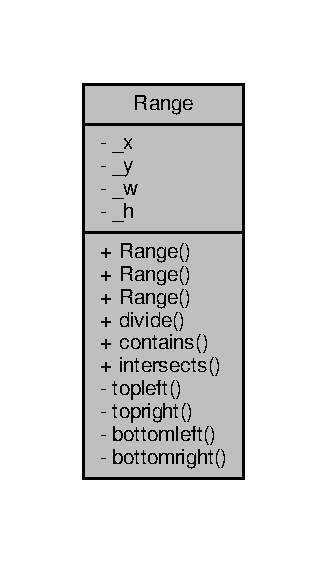
\includegraphics[width=157pt]{classRange__coll__graph}
\end{center}
\end{figure}
\subsection*{Public Member Functions}
\begin{DoxyCompactItemize}
\item 
\hyperlink{classRange_aac818834ebf390ce2b1b8dea544f9123_aac818834ebf390ce2b1b8dea544f9123}{Range} (double w, double h)
\item 
\hyperlink{classRange_a3755a3d0c163bba29d5c7469e15765a0_a3755a3d0c163bba29d5c7469e15765a0}{Range} (double x, double y, double w, double h)
\item 
\hyperlink{classRange_a917b57d9db8d4176bd8963c8cc620d1b_a917b57d9db8d4176bd8963c8cc620d1b}{Range} (const \hyperlink{classRange}{Range} \&)=default
\item 
std\+::tuple$<$ \hyperlink{classRange}{Range}, \hyperlink{classRange}{Range}, \hyperlink{classRange}{Range}, \hyperlink{classRange}{Range} $>$ \hyperlink{classRange_a25a80b49faeb175b80a2028032abbed9_a25a80b49faeb175b80a2028032abbed9}{divide} () const
\item 
bool \hyperlink{classRange_a2d9877708da533077fc2eaeef29b89e4_a2d9877708da533077fc2eaeef29b89e4}{contains} (const \hyperlink{classVect2D}{Vect2D} \&point) const
\item 
bool \hyperlink{classRange_a75debf858d591b0b26ef6215616166a8_a75debf858d591b0b26ef6215616166a8}{intersects} (const \hyperlink{classRange}{Range} \&range) const
\end{DoxyCompactItemize}
\subsection*{Private Member Functions}
\begin{DoxyCompactItemize}
\item 
\hyperlink{classVect2D}{Vect2D} \hyperlink{classRange_ac854e35703f632d845ba8a1ba59f7a4d_ac854e35703f632d845ba8a1ba59f7a4d}{topleft} () const
\item 
\hyperlink{classVect2D}{Vect2D} \hyperlink{classRange_a7b1e4a54c72aa3547b94163a4f74a9b7_a7b1e4a54c72aa3547b94163a4f74a9b7}{topright} () const
\item 
\hyperlink{classVect2D}{Vect2D} \hyperlink{classRange_a60dee0a1d68dd669b2e760d29c7641e7_a60dee0a1d68dd669b2e760d29c7641e7}{bottomleft} () const
\item 
\hyperlink{classVect2D}{Vect2D} \hyperlink{classRange_affd99ce93a18978d79d8c1b4ae8acef9_affd99ce93a18978d79d8c1b4ae8acef9}{bottomright} () const
\end{DoxyCompactItemize}
\subsection*{Private Attributes}
\begin{DoxyCompactItemize}
\item 
double \hyperlink{classRange_a63693ff85463b676ee7451693af5c2c1_a63693ff85463b676ee7451693af5c2c1}{\+\_\+x}
\item 
double \hyperlink{classRange_a5367235978a597b4ff99d50c2e06663c_a5367235978a597b4ff99d50c2e06663c}{\+\_\+y}
\item 
double \hyperlink{classRange_a17489275052a741da3c4f7f287a5bea5_a17489275052a741da3c4f7f287a5bea5}{\+\_\+w}
\item 
double \hyperlink{classRange_aa28af6a934404eae4bc9cb016b48fc60_aa28af6a934404eae4bc9cb016b48fc60}{\+\_\+h}
\end{DoxyCompactItemize}


\subsection{Constructor \& Destructor Documentation}
\mbox{\Hypertarget{classRange_aac818834ebf390ce2b1b8dea544f9123_aac818834ebf390ce2b1b8dea544f9123}\label{classRange_aac818834ebf390ce2b1b8dea544f9123_aac818834ebf390ce2b1b8dea544f9123}} 
\index{Range@{Range}!Range@{Range}}
\index{Range@{Range}!Range@{Range}}
\subsubsection{\texorpdfstring{Range()}{Range()}\hspace{0.1cm}{\footnotesize\ttfamily [1/3]}}
{\footnotesize\ttfamily Range\+::\+Range (\begin{DoxyParamCaption}\item[{double}]{w,  }\item[{double}]{h }\end{DoxyParamCaption})\hspace{0.3cm}{\ttfamily [inline]}}

\mbox{\Hypertarget{classRange_a3755a3d0c163bba29d5c7469e15765a0_a3755a3d0c163bba29d5c7469e15765a0}\label{classRange_a3755a3d0c163bba29d5c7469e15765a0_a3755a3d0c163bba29d5c7469e15765a0}} 
\index{Range@{Range}!Range@{Range}}
\index{Range@{Range}!Range@{Range}}
\subsubsection{\texorpdfstring{Range()}{Range()}\hspace{0.1cm}{\footnotesize\ttfamily [2/3]}}
{\footnotesize\ttfamily Range\+::\+Range (\begin{DoxyParamCaption}\item[{double}]{x,  }\item[{double}]{y,  }\item[{double}]{w,  }\item[{double}]{h }\end{DoxyParamCaption})\hspace{0.3cm}{\ttfamily [inline]}}

\mbox{\Hypertarget{classRange_a917b57d9db8d4176bd8963c8cc620d1b_a917b57d9db8d4176bd8963c8cc620d1b}\label{classRange_a917b57d9db8d4176bd8963c8cc620d1b_a917b57d9db8d4176bd8963c8cc620d1b}} 
\index{Range@{Range}!Range@{Range}}
\index{Range@{Range}!Range@{Range}}
\subsubsection{\texorpdfstring{Range()}{Range()}\hspace{0.1cm}{\footnotesize\ttfamily [3/3]}}
{\footnotesize\ttfamily Range\+::\+Range (\begin{DoxyParamCaption}\item[{const \hyperlink{classRange}{Range} \&}]{ }\end{DoxyParamCaption})\hspace{0.3cm}{\ttfamily [default]}}



\subsection{Member Function Documentation}
\mbox{\Hypertarget{classRange_a60dee0a1d68dd669b2e760d29c7641e7_a60dee0a1d68dd669b2e760d29c7641e7}\label{classRange_a60dee0a1d68dd669b2e760d29c7641e7_a60dee0a1d68dd669b2e760d29c7641e7}} 
\index{Range@{Range}!bottomleft@{bottomleft}}
\index{bottomleft@{bottomleft}!Range@{Range}}
\subsubsection{\texorpdfstring{bottomleft()}{bottomleft()}}
{\footnotesize\ttfamily \hyperlink{classVect2D}{Vect2D} Range\+::bottomleft (\begin{DoxyParamCaption}{ }\end{DoxyParamCaption}) const\hspace{0.3cm}{\ttfamily [inline]}, {\ttfamily [private]}}

\mbox{\Hypertarget{classRange_affd99ce93a18978d79d8c1b4ae8acef9_affd99ce93a18978d79d8c1b4ae8acef9}\label{classRange_affd99ce93a18978d79d8c1b4ae8acef9_affd99ce93a18978d79d8c1b4ae8acef9}} 
\index{Range@{Range}!bottomright@{bottomright}}
\index{bottomright@{bottomright}!Range@{Range}}
\subsubsection{\texorpdfstring{bottomright()}{bottomright()}}
{\footnotesize\ttfamily \hyperlink{classVect2D}{Vect2D} Range\+::bottomright (\begin{DoxyParamCaption}{ }\end{DoxyParamCaption}) const\hspace{0.3cm}{\ttfamily [inline]}, {\ttfamily [private]}}

\mbox{\Hypertarget{classRange_a2d9877708da533077fc2eaeef29b89e4_a2d9877708da533077fc2eaeef29b89e4}\label{classRange_a2d9877708da533077fc2eaeef29b89e4_a2d9877708da533077fc2eaeef29b89e4}} 
\index{Range@{Range}!contains@{contains}}
\index{contains@{contains}!Range@{Range}}
\subsubsection{\texorpdfstring{contains()}{contains()}}
{\footnotesize\ttfamily bool Range\+::contains (\begin{DoxyParamCaption}\item[{const \hyperlink{classVect2D}{Vect2D} \&}]{point }\end{DoxyParamCaption}) const\hspace{0.3cm}{\ttfamily [inline]}}

\mbox{\Hypertarget{classRange_a25a80b49faeb175b80a2028032abbed9_a25a80b49faeb175b80a2028032abbed9}\label{classRange_a25a80b49faeb175b80a2028032abbed9_a25a80b49faeb175b80a2028032abbed9}} 
\index{Range@{Range}!divide@{divide}}
\index{divide@{divide}!Range@{Range}}
\subsubsection{\texorpdfstring{divide()}{divide()}}
{\footnotesize\ttfamily std\+::tuple$<$\hyperlink{classRange}{Range}, \hyperlink{classRange}{Range}, \hyperlink{classRange}{Range}, \hyperlink{classRange}{Range}$>$ Range\+::divide (\begin{DoxyParamCaption}{ }\end{DoxyParamCaption}) const\hspace{0.3cm}{\ttfamily [inline]}}

\mbox{\Hypertarget{classRange_a75debf858d591b0b26ef6215616166a8_a75debf858d591b0b26ef6215616166a8}\label{classRange_a75debf858d591b0b26ef6215616166a8_a75debf858d591b0b26ef6215616166a8}} 
\index{Range@{Range}!intersects@{intersects}}
\index{intersects@{intersects}!Range@{Range}}
\subsubsection{\texorpdfstring{intersects()}{intersects()}}
{\footnotesize\ttfamily bool Range\+::intersects (\begin{DoxyParamCaption}\item[{const \hyperlink{classRange}{Range} \&}]{range }\end{DoxyParamCaption}) const\hspace{0.3cm}{\ttfamily [inline]}}

\mbox{\Hypertarget{classRange_ac854e35703f632d845ba8a1ba59f7a4d_ac854e35703f632d845ba8a1ba59f7a4d}\label{classRange_ac854e35703f632d845ba8a1ba59f7a4d_ac854e35703f632d845ba8a1ba59f7a4d}} 
\index{Range@{Range}!topleft@{topleft}}
\index{topleft@{topleft}!Range@{Range}}
\subsubsection{\texorpdfstring{topleft()}{topleft()}}
{\footnotesize\ttfamily \hyperlink{classVect2D}{Vect2D} Range\+::topleft (\begin{DoxyParamCaption}{ }\end{DoxyParamCaption}) const\hspace{0.3cm}{\ttfamily [inline]}, {\ttfamily [private]}}

\mbox{\Hypertarget{classRange_a7b1e4a54c72aa3547b94163a4f74a9b7_a7b1e4a54c72aa3547b94163a4f74a9b7}\label{classRange_a7b1e4a54c72aa3547b94163a4f74a9b7_a7b1e4a54c72aa3547b94163a4f74a9b7}} 
\index{Range@{Range}!topright@{topright}}
\index{topright@{topright}!Range@{Range}}
\subsubsection{\texorpdfstring{topright()}{topright()}}
{\footnotesize\ttfamily \hyperlink{classVect2D}{Vect2D} Range\+::topright (\begin{DoxyParamCaption}{ }\end{DoxyParamCaption}) const\hspace{0.3cm}{\ttfamily [inline]}, {\ttfamily [private]}}



\subsection{Member Data Documentation}
\mbox{\Hypertarget{classRange_aa28af6a934404eae4bc9cb016b48fc60_aa28af6a934404eae4bc9cb016b48fc60}\label{classRange_aa28af6a934404eae4bc9cb016b48fc60_aa28af6a934404eae4bc9cb016b48fc60}} 
\index{Range@{Range}!\+\_\+h@{\+\_\+h}}
\index{\+\_\+h@{\+\_\+h}!Range@{Range}}
\subsubsection{\texorpdfstring{\+\_\+h}{\_h}}
{\footnotesize\ttfamily double Range\+::\+\_\+h\hspace{0.3cm}{\ttfamily [private]}}

\mbox{\Hypertarget{classRange_a17489275052a741da3c4f7f287a5bea5_a17489275052a741da3c4f7f287a5bea5}\label{classRange_a17489275052a741da3c4f7f287a5bea5_a17489275052a741da3c4f7f287a5bea5}} 
\index{Range@{Range}!\+\_\+w@{\+\_\+w}}
\index{\+\_\+w@{\+\_\+w}!Range@{Range}}
\subsubsection{\texorpdfstring{\+\_\+w}{\_w}}
{\footnotesize\ttfamily double Range\+::\+\_\+w\hspace{0.3cm}{\ttfamily [private]}}

\mbox{\Hypertarget{classRange_a63693ff85463b676ee7451693af5c2c1_a63693ff85463b676ee7451693af5c2c1}\label{classRange_a63693ff85463b676ee7451693af5c2c1_a63693ff85463b676ee7451693af5c2c1}} 
\index{Range@{Range}!\+\_\+x@{\+\_\+x}}
\index{\+\_\+x@{\+\_\+x}!Range@{Range}}
\subsubsection{\texorpdfstring{\+\_\+x}{\_x}}
{\footnotesize\ttfamily double Range\+::\+\_\+x\hspace{0.3cm}{\ttfamily [private]}}

\mbox{\Hypertarget{classRange_a5367235978a597b4ff99d50c2e06663c_a5367235978a597b4ff99d50c2e06663c}\label{classRange_a5367235978a597b4ff99d50c2e06663c_a5367235978a597b4ff99d50c2e06663c}} 
\index{Range@{Range}!\+\_\+y@{\+\_\+y}}
\index{\+\_\+y@{\+\_\+y}!Range@{Range}}
\subsubsection{\texorpdfstring{\+\_\+y}{\_y}}
{\footnotesize\ttfamily double Range\+::\+\_\+y\hspace{0.3cm}{\ttfamily [private]}}



The documentation for this class was generated from the following file\+:\begin{DoxyCompactItemize}
\item 
include/\hyperlink{bsptree_8hpp}{bsptree.\+hpp}\end{DoxyCompactItemize}

\hypertarget{classStamina}{}\section{Stamina Class Reference}
\label{classStamina}\index{Stamina@{Stamina}}


{\ttfamily \#include $<$stamina.\+hpp$>$}



Collaboration diagram for Stamina\+:\nopagebreak
\begin{figure}[H]
\begin{center}
\leavevmode
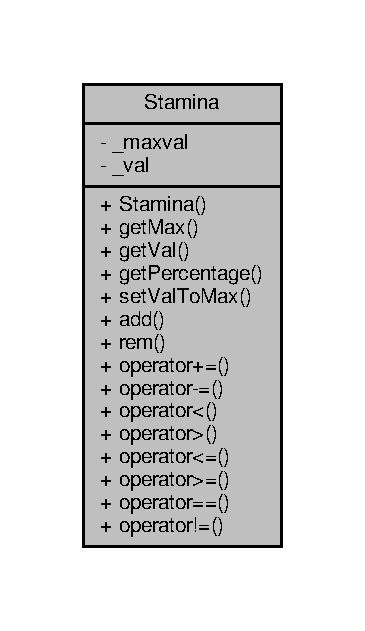
\includegraphics[width=175pt]{classStamina__coll__graph}
\end{center}
\end{figure}
\subsection*{Public Member Functions}
\begin{DoxyCompactItemize}
\item 
\hyperlink{classStamina_a90296cdf856dfd26d661c0bb57b02108_a90296cdf856dfd26d661c0bb57b02108}{Stamina} (double)
\item 
double \hyperlink{classStamina_a2058ea4b530bc666a7ac69fc4549c9fc_a2058ea4b530bc666a7ac69fc4549c9fc}{get\+Max} () const
\item 
double \hyperlink{classStamina_a57bbd8b3071fe52521ddfb084a2c2694_a57bbd8b3071fe52521ddfb084a2c2694}{get\+Val} () const
\item 
double \hyperlink{classStamina_ae828f2e015de23a14150769c0b6c91a6_ae828f2e015de23a14150769c0b6c91a6}{get\+Percentage} () const
\item 
void \hyperlink{classStamina_a8047f55489de6d5101d0c4d1c4ff49b9_a8047f55489de6d5101d0c4d1c4ff49b9}{set\+Val\+To\+Max} ()
\item 
\hyperlink{classStamina}{Stamina} \& \hyperlink{classStamina_afc204ffdbeb2696f031dc68a08c7330c_afc204ffdbeb2696f031dc68a08c7330c}{add} (double)
\item 
\hyperlink{classStamina}{Stamina} \& \hyperlink{classStamina_a54413ab56d9d0782b588eac64ee0bbe0_a54413ab56d9d0782b588eac64ee0bbe0}{rem} (double)
\item 
\hyperlink{classStamina}{Stamina} \& \hyperlink{classStamina_ac6c546b319bdeb9c82f83a0aa87b2894_ac6c546b319bdeb9c82f83a0aa87b2894}{operator+=} (double)
\item 
\hyperlink{classStamina}{Stamina} \& \hyperlink{classStamina_afa57a14ac8fe63c95b9cc1a8ebd66945_afa57a14ac8fe63c95b9cc1a8ebd66945}{operator-\/=} (double)
\item 
bool \hyperlink{classStamina_a4958bdadaf27115a1d458fc94939390a_a4958bdadaf27115a1d458fc94939390a}{operator$<$} (double val) const
\item 
bool \hyperlink{classStamina_aecb929dd6ebe322e92d714fd585413a8_aecb929dd6ebe322e92d714fd585413a8}{operator$>$} (double val) const
\item 
bool \hyperlink{classStamina_a6bdebd03a3310fb1017661c0997484a0_a6bdebd03a3310fb1017661c0997484a0}{operator$<$=} (double val) const
\item 
bool \hyperlink{classStamina_ae0b3f0fe7e80ecaa3e3dcacaa98f79e1_ae0b3f0fe7e80ecaa3e3dcacaa98f79e1}{operator$>$=} (double val) const
\item 
bool \hyperlink{classStamina_aa3067e0326a250c295cfdba2eeb8f8b6_aa3067e0326a250c295cfdba2eeb8f8b6}{operator==} (double val) const
\item 
bool \hyperlink{classStamina_aa8bbeed4d64bf1645b3eeb544bdd2c6a_aa8bbeed4d64bf1645b3eeb544bdd2c6a}{operator!=} (double val) const
\end{DoxyCompactItemize}
\subsection*{Private Attributes}
\begin{DoxyCompactItemize}
\item 
double \hyperlink{classStamina_ada7872b81f23fee639afd0c1ab91ffa8_ada7872b81f23fee639afd0c1ab91ffa8}{\+\_\+maxval}
\item 
double \hyperlink{classStamina_a08f7cc6e531d019ab76269f8fdc1e8a3_a08f7cc6e531d019ab76269f8fdc1e8a3}{\+\_\+val}
\end{DoxyCompactItemize}


\subsection{Constructor \& Destructor Documentation}
\mbox{\Hypertarget{classStamina_a90296cdf856dfd26d661c0bb57b02108_a90296cdf856dfd26d661c0bb57b02108}\label{classStamina_a90296cdf856dfd26d661c0bb57b02108_a90296cdf856dfd26d661c0bb57b02108}} 
\index{Stamina@{Stamina}!Stamina@{Stamina}}
\index{Stamina@{Stamina}!Stamina@{Stamina}}
\subsubsection{\texorpdfstring{Stamina()}{Stamina()}}
{\footnotesize\ttfamily Stamina\+::\+Stamina (\begin{DoxyParamCaption}\item[{double}]{maxval }\end{DoxyParamCaption})\hspace{0.3cm}{\ttfamily [explicit]}}



\subsection{Member Function Documentation}
\mbox{\Hypertarget{classStamina_afc204ffdbeb2696f031dc68a08c7330c_afc204ffdbeb2696f031dc68a08c7330c}\label{classStamina_afc204ffdbeb2696f031dc68a08c7330c_afc204ffdbeb2696f031dc68a08c7330c}} 
\index{Stamina@{Stamina}!add@{add}}
\index{add@{add}!Stamina@{Stamina}}
\subsubsection{\texorpdfstring{add()}{add()}}
{\footnotesize\ttfamily \hyperlink{classStamina}{Stamina} \& Stamina\+::add (\begin{DoxyParamCaption}\item[{double}]{v }\end{DoxyParamCaption})}

\mbox{\Hypertarget{classStamina_a2058ea4b530bc666a7ac69fc4549c9fc_a2058ea4b530bc666a7ac69fc4549c9fc}\label{classStamina_a2058ea4b530bc666a7ac69fc4549c9fc_a2058ea4b530bc666a7ac69fc4549c9fc}} 
\index{Stamina@{Stamina}!get\+Max@{get\+Max}}
\index{get\+Max@{get\+Max}!Stamina@{Stamina}}
\subsubsection{\texorpdfstring{get\+Max()}{getMax()}}
{\footnotesize\ttfamily double Stamina\+::get\+Max (\begin{DoxyParamCaption}{ }\end{DoxyParamCaption}) const}

\mbox{\Hypertarget{classStamina_ae828f2e015de23a14150769c0b6c91a6_ae828f2e015de23a14150769c0b6c91a6}\label{classStamina_ae828f2e015de23a14150769c0b6c91a6_ae828f2e015de23a14150769c0b6c91a6}} 
\index{Stamina@{Stamina}!get\+Percentage@{get\+Percentage}}
\index{get\+Percentage@{get\+Percentage}!Stamina@{Stamina}}
\subsubsection{\texorpdfstring{get\+Percentage()}{getPercentage()}}
{\footnotesize\ttfamily double Stamina\+::get\+Percentage (\begin{DoxyParamCaption}{ }\end{DoxyParamCaption}) const}

\mbox{\Hypertarget{classStamina_a57bbd8b3071fe52521ddfb084a2c2694_a57bbd8b3071fe52521ddfb084a2c2694}\label{classStamina_a57bbd8b3071fe52521ddfb084a2c2694_a57bbd8b3071fe52521ddfb084a2c2694}} 
\index{Stamina@{Stamina}!get\+Val@{get\+Val}}
\index{get\+Val@{get\+Val}!Stamina@{Stamina}}
\subsubsection{\texorpdfstring{get\+Val()}{getVal()}}
{\footnotesize\ttfamily double Stamina\+::get\+Val (\begin{DoxyParamCaption}{ }\end{DoxyParamCaption}) const}

\mbox{\Hypertarget{classStamina_aa8bbeed4d64bf1645b3eeb544bdd2c6a_aa8bbeed4d64bf1645b3eeb544bdd2c6a}\label{classStamina_aa8bbeed4d64bf1645b3eeb544bdd2c6a_aa8bbeed4d64bf1645b3eeb544bdd2c6a}} 
\index{Stamina@{Stamina}!operator"!=@{operator"!=}}
\index{operator"!=@{operator"!=}!Stamina@{Stamina}}
\subsubsection{\texorpdfstring{operator"!=()}{operator!=()}}
{\footnotesize\ttfamily bool Stamina\+::operator!= (\begin{DoxyParamCaption}\item[{double}]{val }\end{DoxyParamCaption}) const}

\mbox{\Hypertarget{classStamina_ac6c546b319bdeb9c82f83a0aa87b2894_ac6c546b319bdeb9c82f83a0aa87b2894}\label{classStamina_ac6c546b319bdeb9c82f83a0aa87b2894_ac6c546b319bdeb9c82f83a0aa87b2894}} 
\index{Stamina@{Stamina}!operator+=@{operator+=}}
\index{operator+=@{operator+=}!Stamina@{Stamina}}
\subsubsection{\texorpdfstring{operator+=()}{operator+=()}}
{\footnotesize\ttfamily \hyperlink{classStamina}{Stamina} \& Stamina\+::operator+= (\begin{DoxyParamCaption}\item[{double}]{v }\end{DoxyParamCaption})}

\mbox{\Hypertarget{classStamina_afa57a14ac8fe63c95b9cc1a8ebd66945_afa57a14ac8fe63c95b9cc1a8ebd66945}\label{classStamina_afa57a14ac8fe63c95b9cc1a8ebd66945_afa57a14ac8fe63c95b9cc1a8ebd66945}} 
\index{Stamina@{Stamina}!operator-\/=@{operator-\/=}}
\index{operator-\/=@{operator-\/=}!Stamina@{Stamina}}
\subsubsection{\texorpdfstring{operator-\/=()}{operator-=()}}
{\footnotesize\ttfamily \hyperlink{classStamina}{Stamina} \& Stamina\+::operator-\/= (\begin{DoxyParamCaption}\item[{double}]{v }\end{DoxyParamCaption})}

\mbox{\Hypertarget{classStamina_a4958bdadaf27115a1d458fc94939390a_a4958bdadaf27115a1d458fc94939390a}\label{classStamina_a4958bdadaf27115a1d458fc94939390a_a4958bdadaf27115a1d458fc94939390a}} 
\index{Stamina@{Stamina}!operator$<$@{operator$<$}}
\index{operator$<$@{operator$<$}!Stamina@{Stamina}}
\subsubsection{\texorpdfstring{operator$<$()}{operator<()}}
{\footnotesize\ttfamily bool Stamina\+::operator$<$ (\begin{DoxyParamCaption}\item[{double}]{val }\end{DoxyParamCaption}) const}

\mbox{\Hypertarget{classStamina_a6bdebd03a3310fb1017661c0997484a0_a6bdebd03a3310fb1017661c0997484a0}\label{classStamina_a6bdebd03a3310fb1017661c0997484a0_a6bdebd03a3310fb1017661c0997484a0}} 
\index{Stamina@{Stamina}!operator$<$=@{operator$<$=}}
\index{operator$<$=@{operator$<$=}!Stamina@{Stamina}}
\subsubsection{\texorpdfstring{operator$<$=()}{operator<=()}}
{\footnotesize\ttfamily bool Stamina\+::operator$<$= (\begin{DoxyParamCaption}\item[{double}]{val }\end{DoxyParamCaption}) const}

\mbox{\Hypertarget{classStamina_aa3067e0326a250c295cfdba2eeb8f8b6_aa3067e0326a250c295cfdba2eeb8f8b6}\label{classStamina_aa3067e0326a250c295cfdba2eeb8f8b6_aa3067e0326a250c295cfdba2eeb8f8b6}} 
\index{Stamina@{Stamina}!operator==@{operator==}}
\index{operator==@{operator==}!Stamina@{Stamina}}
\subsubsection{\texorpdfstring{operator==()}{operator==()}}
{\footnotesize\ttfamily bool Stamina\+::operator== (\begin{DoxyParamCaption}\item[{double}]{val }\end{DoxyParamCaption}) const}

\mbox{\Hypertarget{classStamina_aecb929dd6ebe322e92d714fd585413a8_aecb929dd6ebe322e92d714fd585413a8}\label{classStamina_aecb929dd6ebe322e92d714fd585413a8_aecb929dd6ebe322e92d714fd585413a8}} 
\index{Stamina@{Stamina}!operator$>$@{operator$>$}}
\index{operator$>$@{operator$>$}!Stamina@{Stamina}}
\subsubsection{\texorpdfstring{operator$>$()}{operator>()}}
{\footnotesize\ttfamily bool Stamina\+::operator$>$ (\begin{DoxyParamCaption}\item[{double}]{val }\end{DoxyParamCaption}) const}

\mbox{\Hypertarget{classStamina_ae0b3f0fe7e80ecaa3e3dcacaa98f79e1_ae0b3f0fe7e80ecaa3e3dcacaa98f79e1}\label{classStamina_ae0b3f0fe7e80ecaa3e3dcacaa98f79e1_ae0b3f0fe7e80ecaa3e3dcacaa98f79e1}} 
\index{Stamina@{Stamina}!operator$>$=@{operator$>$=}}
\index{operator$>$=@{operator$>$=}!Stamina@{Stamina}}
\subsubsection{\texorpdfstring{operator$>$=()}{operator>=()}}
{\footnotesize\ttfamily bool Stamina\+::operator$>$= (\begin{DoxyParamCaption}\item[{double}]{val }\end{DoxyParamCaption}) const}

\mbox{\Hypertarget{classStamina_a54413ab56d9d0782b588eac64ee0bbe0_a54413ab56d9d0782b588eac64ee0bbe0}\label{classStamina_a54413ab56d9d0782b588eac64ee0bbe0_a54413ab56d9d0782b588eac64ee0bbe0}} 
\index{Stamina@{Stamina}!rem@{rem}}
\index{rem@{rem}!Stamina@{Stamina}}
\subsubsection{\texorpdfstring{rem()}{rem()}}
{\footnotesize\ttfamily \hyperlink{classStamina}{Stamina} \& Stamina\+::rem (\begin{DoxyParamCaption}\item[{double}]{v }\end{DoxyParamCaption})}

\mbox{\Hypertarget{classStamina_a8047f55489de6d5101d0c4d1c4ff49b9_a8047f55489de6d5101d0c4d1c4ff49b9}\label{classStamina_a8047f55489de6d5101d0c4d1c4ff49b9_a8047f55489de6d5101d0c4d1c4ff49b9}} 
\index{Stamina@{Stamina}!set\+Val\+To\+Max@{set\+Val\+To\+Max}}
\index{set\+Val\+To\+Max@{set\+Val\+To\+Max}!Stamina@{Stamina}}
\subsubsection{\texorpdfstring{set\+Val\+To\+Max()}{setValToMax()}}
{\footnotesize\ttfamily void Stamina\+::set\+Val\+To\+Max (\begin{DoxyParamCaption}{ }\end{DoxyParamCaption})}



\subsection{Member Data Documentation}
\mbox{\Hypertarget{classStamina_ada7872b81f23fee639afd0c1ab91ffa8_ada7872b81f23fee639afd0c1ab91ffa8}\label{classStamina_ada7872b81f23fee639afd0c1ab91ffa8_ada7872b81f23fee639afd0c1ab91ffa8}} 
\index{Stamina@{Stamina}!\+\_\+maxval@{\+\_\+maxval}}
\index{\+\_\+maxval@{\+\_\+maxval}!Stamina@{Stamina}}
\subsubsection{\texorpdfstring{\+\_\+maxval}{\_maxval}}
{\footnotesize\ttfamily double Stamina\+::\+\_\+maxval\hspace{0.3cm}{\ttfamily [private]}}

\mbox{\Hypertarget{classStamina_a08f7cc6e531d019ab76269f8fdc1e8a3_a08f7cc6e531d019ab76269f8fdc1e8a3}\label{classStamina_a08f7cc6e531d019ab76269f8fdc1e8a3_a08f7cc6e531d019ab76269f8fdc1e8a3}} 
\index{Stamina@{Stamina}!\+\_\+val@{\+\_\+val}}
\index{\+\_\+val@{\+\_\+val}!Stamina@{Stamina}}
\subsubsection{\texorpdfstring{\+\_\+val}{\_val}}
{\footnotesize\ttfamily double Stamina\+::\+\_\+val\hspace{0.3cm}{\ttfamily [private]}}



The documentation for this class was generated from the following files\+:\begin{DoxyCompactItemize}
\item 
include/\hyperlink{stamina_8hpp}{stamina.\+hpp}\item 
src/\hyperlink{stamina_8cpp}{stamina.\+cpp}\end{DoxyCompactItemize}

\hypertarget{classVect2D}{}\section{Vect2D Class Reference}
\label{classVect2D}\index{Vect2D@{Vect2D}}


{\ttfamily \#include $<$vect2d.\+hpp$>$}



Collaboration diagram for Vect2D\+:\nopagebreak
\begin{figure}[H]
\begin{center}
\leavevmode
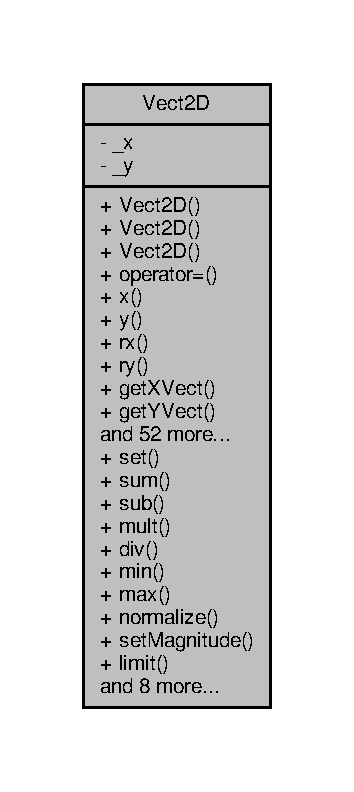
\includegraphics[width=170pt]{classVect2D__coll__graph}
\end{center}
\end{figure}
\subsection*{Public Member Functions}
\begin{DoxyCompactItemize}
\item 
\hyperlink{classVect2D_a6c93f0ad4edc535515d33f8e8f6b7842_a6c93f0ad4edc535515d33f8e8f6b7842}{Vect2D} ()
\item 
\hyperlink{classVect2D_ac977f3d217a9ad80f39fcf28a7b217f3_ac977f3d217a9ad80f39fcf28a7b217f3}{Vect2D} (double \hyperlink{classVect2D_a5ec56ffcb57f5dc61cb24a8672bfa196_a5ec56ffcb57f5dc61cb24a8672bfa196}{x}, double \hyperlink{classVect2D_ad0ca2a82c313cfa471e0339bafc635e9_ad0ca2a82c313cfa471e0339bafc635e9}{y})
\item 
\hyperlink{classVect2D_a2875ad36fed58a50922cda20f0e42afc_a2875ad36fed58a50922cda20f0e42afc}{Vect2D} (const \hyperlink{classVect2D}{Vect2D} \&v)
\item 
\hyperlink{classVect2D}{Vect2D} \& \hyperlink{classVect2D_ac64ef2415eabdf79c587c71a2f727701_ac64ef2415eabdf79c587c71a2f727701}{operator=} (const \hyperlink{classVect2D}{Vect2D} \&)
\item 
double \hyperlink{classVect2D_a5ec56ffcb57f5dc61cb24a8672bfa196_a5ec56ffcb57f5dc61cb24a8672bfa196}{x} () const
\item 
double \hyperlink{classVect2D_ad0ca2a82c313cfa471e0339bafc635e9_ad0ca2a82c313cfa471e0339bafc635e9}{y} () const
\item 
double \& \hyperlink{classVect2D_a157a80045188c626d2a582aa5b42ea09_a157a80045188c626d2a582aa5b42ea09}{rx} ()
\item 
double \& \hyperlink{classVect2D_ab29c733af56363e7b640d53114fdb797_ab29c733af56363e7b640d53114fdb797}{ry} ()
\item 
\hyperlink{classVect2D}{Vect2D} \hyperlink{classVect2D_a1bf72f44ebf9444c5f52a6499dc8dcb3_a1bf72f44ebf9444c5f52a6499dc8dcb3}{get\+X\+Vect} () const
\item 
\hyperlink{classVect2D}{Vect2D} \hyperlink{classVect2D_a13e0a84562e7b1ebef4a530aaacfa060_a13e0a84562e7b1ebef4a530aaacfa060}{get\+Y\+Vect} () const
\item 
std\+::pair$<$ double, double $>$ \hyperlink{classVect2D_a347f48c0f8fb2f05592251f78be33a5c_a347f48c0f8fb2f05592251f78be33a5c}{get\+Pair} () const
\item 
\hyperlink{classVect2D}{Vect2D} \& \hyperlink{classVect2D_a0dd170984a57bb034ccf4f939bedf117_a0dd170984a57bb034ccf4f939bedf117}{set} (double, double)
\item 
\hyperlink{classVect2D}{Vect2D} \& \hyperlink{classVect2D_a24dda506fe6172d30e199e3b9949b9c4_a24dda506fe6172d30e199e3b9949b9c4}{add} (const \hyperlink{classVect2D}{Vect2D} \&)
\item 
\hyperlink{classVect2D}{Vect2D} \& \hyperlink{classVect2D_a14a3e3096417062b3a6e30d2a49e5500_a14a3e3096417062b3a6e30d2a49e5500}{rem} (const \hyperlink{classVect2D}{Vect2D} \&)
\item 
\hyperlink{classVect2D}{Vect2D} \& \hyperlink{classVect2D_aa6c72498622bb2c4796c10c237ba4099_aa6c72498622bb2c4796c10c237ba4099}{mult} (double)
\item 
\hyperlink{classVect2D}{Vect2D} \& \hyperlink{classVect2D_a201bc18b8e38a4b3e16aa02b9b780e81_a201bc18b8e38a4b3e16aa02b9b780e81}{div} (double)
\item 
\hyperlink{classVect2D}{Vect2D} \& \hyperlink{classVect2D_a4c048721a9f0c03cf11adf2d48570c95_a4c048721a9f0c03cf11adf2d48570c95}{min} (\hyperlink{classVect2D}{Vect2D} \&)
\item 
\hyperlink{classVect2D}{Vect2D} \& \hyperlink{classVect2D_ad9b9161966bf86c80adffb02292b43c2_ad9b9161966bf86c80adffb02292b43c2}{max} (\hyperlink{classVect2D}{Vect2D} \&)
\item 
\hyperlink{classVect2D}{Vect2D} \& \hyperlink{classVect2D_a48cac0dc85a710d0437b89c3059a241e_a48cac0dc85a710d0437b89c3059a241e}{normalize} ()
\item 
\hyperlink{classVect2D}{Vect2D} \& \hyperlink{classVect2D_a5e667df64c385e50c1aecc977dc09e27_a5e667df64c385e50c1aecc977dc09e27}{set\+Magnitude} (double)
\item 
\hyperlink{classVect2D}{Vect2D} \& \hyperlink{classVect2D_a9836fb1bf48b847984cf438a6d48f9c2_a9836fb1bf48b847984cf438a6d48f9c2}{limit} (const \hyperlink{classVect2D}{Vect2D} \&)
\item 
\hyperlink{classVect2D}{Vect2D} \& \hyperlink{classVect2D_af466e97d95d8cd0b3240739ca8a351ab_af466e97d95d8cd0b3240739ca8a351ab}{limit} (double)
\item 
\hyperlink{classVect2D}{Vect2D} \& \hyperlink{classVect2D_a8f348f466abb7b7eee560cbb532e0b81_a8f348f466abb7b7eee560cbb532e0b81}{bounds} (const \hyperlink{classVect2D}{Vect2D} \&)
\item 
\hyperlink{classVect2D}{Vect2D} \& \hyperlink{classVect2D_aa0f8430574aeb390f0c625c9aed19f53_aa0f8430574aeb390f0c625c9aed19f53}{rotate} (double)
\item 
\hyperlink{classVect2D}{Vect2D} \& \hyperlink{classVect2D_af5b0305051ba2c3f97cfb2d49035ba97_af5b0305051ba2c3f97cfb2d49035ba97}{rotate\+Deg} (double)
\item 
\hyperlink{classVect2D}{Vect2D} \hyperlink{classVect2D_a8bf790204c1b93b6569cbe8eb5fd1e0f_a8bf790204c1b93b6569cbe8eb5fd1e0f}{set} (double, double) const
\item 
\hyperlink{classVect2D}{Vect2D} \hyperlink{classVect2D_abae2f22236c825a3fb1dfdc434ae1f45_abae2f22236c825a3fb1dfdc434ae1f45}{add} (const \hyperlink{classVect2D}{Vect2D} \&) const
\item 
\hyperlink{classVect2D}{Vect2D} \hyperlink{classVect2D_a7986c5c040e6ba8ad2e44bdbdd6177b6_a7986c5c040e6ba8ad2e44bdbdd6177b6}{rem} (const \hyperlink{classVect2D}{Vect2D} \&) const
\item 
\hyperlink{classVect2D}{Vect2D} \hyperlink{classVect2D_ac7672052c102f5ee2e4f4582af27264e_ac7672052c102f5ee2e4f4582af27264e}{mult} (double) const
\item 
\hyperlink{classVect2D}{Vect2D} \hyperlink{classVect2D_a0abf4b83be014c545a7a90a0ea165632_a0abf4b83be014c545a7a90a0ea165632}{div} (double) const
\item 
\hyperlink{classVect2D}{Vect2D} \hyperlink{classVect2D_a7c7e91d06c0cebad78acf57664ff3207_a7c7e91d06c0cebad78acf57664ff3207}{min} (\hyperlink{classVect2D}{Vect2D} \&) const
\item 
\hyperlink{classVect2D}{Vect2D} \hyperlink{classVect2D_a16316306d609d1e7594f747632ada546_a16316306d609d1e7594f747632ada546}{max} (\hyperlink{classVect2D}{Vect2D} \&) const
\item 
\hyperlink{classVect2D}{Vect2D} \hyperlink{classVect2D_a81341d9ac6fae20c826302a547b0996d_a81341d9ac6fae20c826302a547b0996d}{normalize} () const
\item 
\hyperlink{classVect2D}{Vect2D} \hyperlink{classVect2D_a0144b24b02992650fe84a6f8d6bcbfb5_a0144b24b02992650fe84a6f8d6bcbfb5}{set\+Magnitude} (double) const
\item 
\hyperlink{classVect2D}{Vect2D} \hyperlink{classVect2D_a1a3e45f232ff6e5a4f2894100c5246bf_a1a3e45f232ff6e5a4f2894100c5246bf}{limit} (double) const
\item 
\hyperlink{classVect2D}{Vect2D} \hyperlink{classVect2D_a2c297e74ea6bc349ba3b31793b11404b_a2c297e74ea6bc349ba3b31793b11404b}{bounds} (const \hyperlink{classVect2D}{Vect2D} \&) const
\item 
\hyperlink{classVect2D}{Vect2D} \hyperlink{classVect2D_a436ad92b224172b8bed995bade778126_a436ad92b224172b8bed995bade778126}{rotate} (double) const
\item 
\hyperlink{classVect2D}{Vect2D} \hyperlink{classVect2D_ab02782179e127d49dc292504b498b6b6_ab02782179e127d49dc292504b498b6b6}{rotate\+Deg} (double) const
\item 
double \hyperlink{classVect2D_af4bc907b1b4fbb628ddd126ac82cc49f_af4bc907b1b4fbb628ddd126ac82cc49f}{mag} () const
\item 
double \hyperlink{classVect2D_a059c879cc608a079caf62658693d4a11_a059c879cc608a079caf62658693d4a11}{dot} (const \hyperlink{classVect2D}{Vect2D} \&) const
\item 
double \hyperlink{classVect2D_a8aadc1aa9001b599513a3cddc3da4fec_a8aadc1aa9001b599513a3cddc3da4fec}{distance} (const \hyperlink{classVect2D}{Vect2D} \&) const
\item 
double \hyperlink{classVect2D_ab1be9b2af5abce11bc0cbb73a76aeaa5_ab1be9b2af5abce11bc0cbb73a76aeaa5}{angle\+Rad} () const
\item 
double \hyperlink{classVect2D_a13ca3566f8ff594598bba9e08fcbc88c_a13ca3566f8ff594598bba9e08fcbc88c}{angle\+Deg} () const
\item 
double \hyperlink{classVect2D_ac8a3f1678a112188aefec21320a66b49_ac8a3f1678a112188aefec21320a66b49}{angle\+Between\+Rad} (const \hyperlink{classVect2D}{Vect2D} \&) const
\item 
double \hyperlink{classVect2D_adb36bba502eb3e28e01fea196c2a2387_adb36bba502eb3e28e01fea196c2a2387}{angle\+Between\+Deg} (const \hyperlink{classVect2D}{Vect2D} \&) const
\item 
\hyperlink{classVect2D}{Vect2D} \hyperlink{classVect2D_a1774995c73b39f2cccd5a2307a52e1bd_a1774995c73b39f2cccd5a2307a52e1bd}{scalar\+Projection} (const \hyperlink{classVect2D}{Vect2D} \&) const
\item 
\hyperlink{classVect2D}{Vect2D} \hyperlink{classVect2D_a85276732f66c0ffe964eb3e3b5795a73_a85276732f66c0ffe964eb3e3b5795a73}{operator+} (const \hyperlink{classVect2D}{Vect2D} \&) const
\item 
\hyperlink{classVect2D}{Vect2D} \hyperlink{classVect2D_ab66937f68aab4d05cabb491e532b5359_ab66937f68aab4d05cabb491e532b5359}{operator-\/} (const \hyperlink{classVect2D}{Vect2D} \&) const
\item 
\hyperlink{classVect2D}{Vect2D} \hyperlink{classVect2D_a8813ae819872f90d908968760b2c6730_a8813ae819872f90d908968760b2c6730}{operator$\ast$} (double) const
\item 
\hyperlink{classVect2D}{Vect2D} \hyperlink{classVect2D_a208f651c84afb4e7b655eb8f964efe23_a208f651c84afb4e7b655eb8f964efe23}{operator/} (double) const
\item 
\hyperlink{classVect2D}{Vect2D} \hyperlink{classVect2D_a043d37b85822f15af552c2c08b2436fa_a043d37b85822f15af552c2c08b2436fa}{operator-\/} () const
\item 
\hyperlink{classVect2D}{Vect2D} \& \hyperlink{classVect2D_ac4a0c9f90498d4745557bfd67da88f2d_ac4a0c9f90498d4745557bfd67da88f2d}{operator+=} (const \hyperlink{classVect2D}{Vect2D} \&)
\item 
\hyperlink{classVect2D}{Vect2D} \& \hyperlink{classVect2D_a8513ee56819d5becc5d486acf16f78ed_a8513ee56819d5becc5d486acf16f78ed}{operator-\/=} (const \hyperlink{classVect2D}{Vect2D} \&)
\item 
\hyperlink{classVect2D}{Vect2D} \& \hyperlink{classVect2D_ac5988c6f0333458d3eac708e4d96e378_ac5988c6f0333458d3eac708e4d96e378}{operator$\ast$=} (double)
\item 
\hyperlink{classVect2D}{Vect2D} \& \hyperlink{classVect2D_a3b7548e38f4b0dc4df235cc71b20492b_a3b7548e38f4b0dc4df235cc71b20492b}{operator/=} (double)
\item 
bool \hyperlink{classVect2D_a22aecc87e1f93ef47761421b138c0f21_a22aecc87e1f93ef47761421b138c0f21}{operator$>$} (const \hyperlink{classVect2D}{Vect2D} \&) const
\item 
bool \hyperlink{classVect2D_a244c5937db2e35a99eeed4d3af2e9663_a244c5937db2e35a99eeed4d3af2e9663}{operator$>$=} (const \hyperlink{classVect2D}{Vect2D} \&) const
\item 
bool \hyperlink{classVect2D_acf1966ca9b29afb6ddf7900b6d471e28_acf1966ca9b29afb6ddf7900b6d471e28}{operator$<$} (const \hyperlink{classVect2D}{Vect2D} \&) const
\item 
bool \hyperlink{classVect2D_ae2d571e20a3332e68e8289e7683c8dc7_ae2d571e20a3332e68e8289e7683c8dc7}{operator$<$=} (const \hyperlink{classVect2D}{Vect2D} \&) const
\item 
bool \hyperlink{classVect2D_a90c23632f377ade5b4f59b226bc6d934_a90c23632f377ade5b4f59b226bc6d934}{operator==} (const \hyperlink{classVect2D}{Vect2D} \&) const
\item 
bool \hyperlink{classVect2D_a94963287794e76b9a511fb5f766d9082_a94963287794e76b9a511fb5f766d9082}{operator!=} (const \hyperlink{classVect2D}{Vect2D} \&) const
\item 
\hyperlink{classVect2D_adc9809c2f646699cc2a1b43936b5caf3_adc9809c2f646699cc2a1b43936b5caf3}{operator std\+::pair$<$ double, double $>$} () const
\end{DoxyCompactItemize}
\subsection*{Static Public Member Functions}
\begin{DoxyCompactItemize}
\item 
static \hyperlink{classVect2D}{Vect2D} \hyperlink{classVect2D_a713fc308bd6d3efef5ff9d5b5e9ae426_a713fc308bd6d3efef5ff9d5b5e9ae426}{set} (const \hyperlink{classVect2D}{Vect2D} \&, double, double)
\item 
static \hyperlink{classVect2D}{Vect2D} \hyperlink{classVect2D_a41c1598c79a24bf2d819f2762cb83d58_a41c1598c79a24bf2d819f2762cb83d58}{sum} (const \hyperlink{classVect2D}{Vect2D} \&, const \hyperlink{classVect2D}{Vect2D} \&)
\item 
static \hyperlink{classVect2D}{Vect2D} \hyperlink{classVect2D_a338c5688a1264ece021066dff5c96f32_a338c5688a1264ece021066dff5c96f32}{sub} (const \hyperlink{classVect2D}{Vect2D} \&, const \hyperlink{classVect2D}{Vect2D} \&)
\item 
static \hyperlink{classVect2D}{Vect2D} \hyperlink{classVect2D_a4036230e4f31e21784c268fc02dcd090_a4036230e4f31e21784c268fc02dcd090}{mult} (const \hyperlink{classVect2D}{Vect2D} \&, double)
\item 
static \hyperlink{classVect2D}{Vect2D} \hyperlink{classVect2D_a6e1503bbca56226b6f942ea63c5fbbff_a6e1503bbca56226b6f942ea63c5fbbff}{div} (const \hyperlink{classVect2D}{Vect2D} \&, double)
\item 
static \hyperlink{classVect2D}{Vect2D} \hyperlink{classVect2D_abfce9e126bec3019747932c0fd9ef951_abfce9e126bec3019747932c0fd9ef951}{min} (\hyperlink{classVect2D}{Vect2D} \&, \hyperlink{classVect2D}{Vect2D} \&)
\item 
static \hyperlink{classVect2D}{Vect2D} \hyperlink{classVect2D_a65d0e20a2cc8b7cc7670e830c74f1457_a65d0e20a2cc8b7cc7670e830c74f1457}{max} (\hyperlink{classVect2D}{Vect2D} \&, \hyperlink{classVect2D}{Vect2D} \&)
\item 
static \hyperlink{classVect2D}{Vect2D} \hyperlink{classVect2D_a942fc02dc6fca9d2d9170316300d5d7f_a942fc02dc6fca9d2d9170316300d5d7f}{normalize} (const \hyperlink{classVect2D}{Vect2D} \&)
\item 
static \hyperlink{classVect2D}{Vect2D} \hyperlink{classVect2D_a2d33dc31e186617af5a6919f1e94e39f_a2d33dc31e186617af5a6919f1e94e39f}{set\+Magnitude} (const \hyperlink{classVect2D}{Vect2D} \&, double)
\item 
static \hyperlink{classVect2D}{Vect2D} \hyperlink{classVect2D_a06e0fccb35246c39442b68a675ed1aca_a06e0fccb35246c39442b68a675ed1aca}{limit} (const \hyperlink{classVect2D}{Vect2D} \&, double)
\item 
static \hyperlink{classVect2D}{Vect2D} \hyperlink{classVect2D_ac609c29d60516b1c802be365635a1c4b_ac609c29d60516b1c802be365635a1c4b}{rotate} (const \hyperlink{classVect2D}{Vect2D} \&, double)
\item 
static \hyperlink{classVect2D}{Vect2D} \hyperlink{classVect2D_a9b5ef5a8c654231b3c481f715d4210d5_a9b5ef5a8c654231b3c481f715d4210d5}{rotate\+Deg} (const \hyperlink{classVect2D}{Vect2D} \&, double)
\item 
static double \hyperlink{classVect2D_a376f089a44760de2d73939e5cbd603d0_a376f089a44760de2d73939e5cbd603d0}{mag} (const \hyperlink{classVect2D}{Vect2D} \&)
\item 
static double \hyperlink{classVect2D_a46b44def87620ebfe9991514a544d3a4_a46b44def87620ebfe9991514a544d3a4}{dot} (const \hyperlink{classVect2D}{Vect2D} \&, const \hyperlink{classVect2D}{Vect2D} \&)
\item 
static double \hyperlink{classVect2D_afc6a031b9dd2200be039def103dcd1c8_afc6a031b9dd2200be039def103dcd1c8}{distance} (const \hyperlink{classVect2D}{Vect2D} \&, const \hyperlink{classVect2D}{Vect2D} \&)
\item 
static double \hyperlink{classVect2D_a3f8039dc87affb32f851b1937a1fa2fd_a3f8039dc87affb32f851b1937a1fa2fd}{angle\+Between\+Rad} (const \hyperlink{classVect2D}{Vect2D} \&, const \hyperlink{classVect2D}{Vect2D} \&)
\item 
static double \hyperlink{classVect2D_a29c384be9242c7426b2a5d330fe78a08_a29c384be9242c7426b2a5d330fe78a08}{angle\+Between\+Deg} (const \hyperlink{classVect2D}{Vect2D} \&, const \hyperlink{classVect2D}{Vect2D} \&)
\item 
static \hyperlink{classVect2D}{Vect2D} \hyperlink{classVect2D_aee86f314ed5020f7dada62cf2b29a532_aee86f314ed5020f7dada62cf2b29a532}{scalar\+Projection} (const \hyperlink{classVect2D}{Vect2D} \&, const \hyperlink{classVect2D}{Vect2D} \&)
\end{DoxyCompactItemize}
\subsection*{Private Attributes}
\begin{DoxyCompactItemize}
\item 
double \hyperlink{classVect2D_aa41c2c1afe6d0ac0cf18b5fdc9e98721_aa41c2c1afe6d0ac0cf18b5fdc9e98721}{\+\_\+x}
\item 
double \hyperlink{classVect2D_a0191f309063b9219ea38d5eb24e55e42_a0191f309063b9219ea38d5eb24e55e42}{\+\_\+y}
\end{DoxyCompactItemize}
\subsection*{Friends}
\begin{DoxyCompactItemize}
\item 
\hyperlink{classVect2D}{Vect2D} \hyperlink{classVect2D_a48631d6a1c75eb08d287e3c4c4e3c95e_a48631d6a1c75eb08d287e3c4c4e3c95e}{operator$\ast$} (double, const \hyperlink{classVect2D}{Vect2D} \&)
\item 
\hyperlink{classVect2D}{Vect2D} \hyperlink{classVect2D_a024a271ab52db1ae67332c062797f6f4_a024a271ab52db1ae67332c062797f6f4}{operator/} (double, const \hyperlink{classVect2D}{Vect2D} \&)
\item 
std\+::ostream \& \hyperlink{classVect2D_a7e68af9444ebe81a72ba4eec633f4d65_a7e68af9444ebe81a72ba4eec633f4d65}{operator$<$$<$} (std\+::ostream \&os, const \hyperlink{classVect2D}{Vect2D} \&)
\item 
std\+::istream \& \hyperlink{classVect2D_ad8969df375ebf041a3f9ccdb635357fd_ad8969df375ebf041a3f9ccdb635357fd}{operator$>$$>$} (std\+::istream \&is, const \hyperlink{classVect2D}{Vect2D} \&)
\end{DoxyCompactItemize}


\subsection{Constructor \& Destructor Documentation}
\mbox{\Hypertarget{classVect2D_a6c93f0ad4edc535515d33f8e8f6b7842_a6c93f0ad4edc535515d33f8e8f6b7842}\label{classVect2D_a6c93f0ad4edc535515d33f8e8f6b7842_a6c93f0ad4edc535515d33f8e8f6b7842}} 
\index{Vect2D@{Vect2D}!Vect2D@{Vect2D}}
\index{Vect2D@{Vect2D}!Vect2D@{Vect2D}}
\subsubsection{\texorpdfstring{Vect2\+D()}{Vect2D()}\hspace{0.1cm}{\footnotesize\ttfamily [1/3]}}
{\footnotesize\ttfamily Vect2\+D\+::\+Vect2D (\begin{DoxyParamCaption}{ }\end{DoxyParamCaption})}

\mbox{\Hypertarget{classVect2D_ac977f3d217a9ad80f39fcf28a7b217f3_ac977f3d217a9ad80f39fcf28a7b217f3}\label{classVect2D_ac977f3d217a9ad80f39fcf28a7b217f3_ac977f3d217a9ad80f39fcf28a7b217f3}} 
\index{Vect2D@{Vect2D}!Vect2D@{Vect2D}}
\index{Vect2D@{Vect2D}!Vect2D@{Vect2D}}
\subsubsection{\texorpdfstring{Vect2\+D()}{Vect2D()}\hspace{0.1cm}{\footnotesize\ttfamily [2/3]}}
{\footnotesize\ttfamily Vect2\+D\+::\+Vect2D (\begin{DoxyParamCaption}\item[{double}]{x,  }\item[{double}]{y }\end{DoxyParamCaption})}

\mbox{\Hypertarget{classVect2D_a2875ad36fed58a50922cda20f0e42afc_a2875ad36fed58a50922cda20f0e42afc}\label{classVect2D_a2875ad36fed58a50922cda20f0e42afc_a2875ad36fed58a50922cda20f0e42afc}} 
\index{Vect2D@{Vect2D}!Vect2D@{Vect2D}}
\index{Vect2D@{Vect2D}!Vect2D@{Vect2D}}
\subsubsection{\texorpdfstring{Vect2\+D()}{Vect2D()}\hspace{0.1cm}{\footnotesize\ttfamily [3/3]}}
{\footnotesize\ttfamily Vect2\+D\+::\+Vect2D (\begin{DoxyParamCaption}\item[{const \hyperlink{classVect2D}{Vect2D} \&}]{v }\end{DoxyParamCaption})}



\subsection{Member Function Documentation}
\mbox{\Hypertarget{classVect2D_a24dda506fe6172d30e199e3b9949b9c4_a24dda506fe6172d30e199e3b9949b9c4}\label{classVect2D_a24dda506fe6172d30e199e3b9949b9c4_a24dda506fe6172d30e199e3b9949b9c4}} 
\index{Vect2D@{Vect2D}!add@{add}}
\index{add@{add}!Vect2D@{Vect2D}}
\subsubsection{\texorpdfstring{add()}{add()}\hspace{0.1cm}{\footnotesize\ttfamily [1/2]}}
{\footnotesize\ttfamily \hyperlink{classVect2D}{Vect2D} \& Vect2\+D\+::add (\begin{DoxyParamCaption}\item[{const \hyperlink{classVect2D}{Vect2D} \&}]{v }\end{DoxyParamCaption})}

\mbox{\Hypertarget{classVect2D_abae2f22236c825a3fb1dfdc434ae1f45_abae2f22236c825a3fb1dfdc434ae1f45}\label{classVect2D_abae2f22236c825a3fb1dfdc434ae1f45_abae2f22236c825a3fb1dfdc434ae1f45}} 
\index{Vect2D@{Vect2D}!add@{add}}
\index{add@{add}!Vect2D@{Vect2D}}
\subsubsection{\texorpdfstring{add()}{add()}\hspace{0.1cm}{\footnotesize\ttfamily [2/2]}}
{\footnotesize\ttfamily \hyperlink{classVect2D}{Vect2D} Vect2\+D\+::add (\begin{DoxyParamCaption}\item[{const \hyperlink{classVect2D}{Vect2D} \&}]{v }\end{DoxyParamCaption}) const}

\mbox{\Hypertarget{classVect2D_adb36bba502eb3e28e01fea196c2a2387_adb36bba502eb3e28e01fea196c2a2387}\label{classVect2D_adb36bba502eb3e28e01fea196c2a2387_adb36bba502eb3e28e01fea196c2a2387}} 
\index{Vect2D@{Vect2D}!angle\+Between\+Deg@{angle\+Between\+Deg}}
\index{angle\+Between\+Deg@{angle\+Between\+Deg}!Vect2D@{Vect2D}}
\subsubsection{\texorpdfstring{angle\+Between\+Deg()}{angleBetweenDeg()}\hspace{0.1cm}{\footnotesize\ttfamily [1/2]}}
{\footnotesize\ttfamily double Vect2\+D\+::angle\+Between\+Deg (\begin{DoxyParamCaption}\item[{const \hyperlink{classVect2D}{Vect2D} \&}]{v }\end{DoxyParamCaption}) const}

\mbox{\Hypertarget{classVect2D_a29c384be9242c7426b2a5d330fe78a08_a29c384be9242c7426b2a5d330fe78a08}\label{classVect2D_a29c384be9242c7426b2a5d330fe78a08_a29c384be9242c7426b2a5d330fe78a08}} 
\index{Vect2D@{Vect2D}!angle\+Between\+Deg@{angle\+Between\+Deg}}
\index{angle\+Between\+Deg@{angle\+Between\+Deg}!Vect2D@{Vect2D}}
\subsubsection{\texorpdfstring{angle\+Between\+Deg()}{angleBetweenDeg()}\hspace{0.1cm}{\footnotesize\ttfamily [2/2]}}
{\footnotesize\ttfamily double Vect2\+D\+::angle\+Between\+Deg (\begin{DoxyParamCaption}\item[{const \hyperlink{classVect2D}{Vect2D} \&}]{v1,  }\item[{const \hyperlink{classVect2D}{Vect2D} \&}]{v2 }\end{DoxyParamCaption})\hspace{0.3cm}{\ttfamily [static]}}

\mbox{\Hypertarget{classVect2D_ac8a3f1678a112188aefec21320a66b49_ac8a3f1678a112188aefec21320a66b49}\label{classVect2D_ac8a3f1678a112188aefec21320a66b49_ac8a3f1678a112188aefec21320a66b49}} 
\index{Vect2D@{Vect2D}!angle\+Between\+Rad@{angle\+Between\+Rad}}
\index{angle\+Between\+Rad@{angle\+Between\+Rad}!Vect2D@{Vect2D}}
\subsubsection{\texorpdfstring{angle\+Between\+Rad()}{angleBetweenRad()}\hspace{0.1cm}{\footnotesize\ttfamily [1/2]}}
{\footnotesize\ttfamily double Vect2\+D\+::angle\+Between\+Rad (\begin{DoxyParamCaption}\item[{const \hyperlink{classVect2D}{Vect2D} \&}]{v }\end{DoxyParamCaption}) const}

\mbox{\Hypertarget{classVect2D_a3f8039dc87affb32f851b1937a1fa2fd_a3f8039dc87affb32f851b1937a1fa2fd}\label{classVect2D_a3f8039dc87affb32f851b1937a1fa2fd_a3f8039dc87affb32f851b1937a1fa2fd}} 
\index{Vect2D@{Vect2D}!angle\+Between\+Rad@{angle\+Between\+Rad}}
\index{angle\+Between\+Rad@{angle\+Between\+Rad}!Vect2D@{Vect2D}}
\subsubsection{\texorpdfstring{angle\+Between\+Rad()}{angleBetweenRad()}\hspace{0.1cm}{\footnotesize\ttfamily [2/2]}}
{\footnotesize\ttfamily double Vect2\+D\+::angle\+Between\+Rad (\begin{DoxyParamCaption}\item[{const \hyperlink{classVect2D}{Vect2D} \&}]{v1,  }\item[{const \hyperlink{classVect2D}{Vect2D} \&}]{v2 }\end{DoxyParamCaption})\hspace{0.3cm}{\ttfamily [static]}}

\mbox{\Hypertarget{classVect2D_a13ca3566f8ff594598bba9e08fcbc88c_a13ca3566f8ff594598bba9e08fcbc88c}\label{classVect2D_a13ca3566f8ff594598bba9e08fcbc88c_a13ca3566f8ff594598bba9e08fcbc88c}} 
\index{Vect2D@{Vect2D}!angle\+Deg@{angle\+Deg}}
\index{angle\+Deg@{angle\+Deg}!Vect2D@{Vect2D}}
\subsubsection{\texorpdfstring{angle\+Deg()}{angleDeg()}}
{\footnotesize\ttfamily double Vect2\+D\+::angle\+Deg (\begin{DoxyParamCaption}{ }\end{DoxyParamCaption}) const}

\mbox{\Hypertarget{classVect2D_ab1be9b2af5abce11bc0cbb73a76aeaa5_ab1be9b2af5abce11bc0cbb73a76aeaa5}\label{classVect2D_ab1be9b2af5abce11bc0cbb73a76aeaa5_ab1be9b2af5abce11bc0cbb73a76aeaa5}} 
\index{Vect2D@{Vect2D}!angle\+Rad@{angle\+Rad}}
\index{angle\+Rad@{angle\+Rad}!Vect2D@{Vect2D}}
\subsubsection{\texorpdfstring{angle\+Rad()}{angleRad()}}
{\footnotesize\ttfamily double Vect2\+D\+::angle\+Rad (\begin{DoxyParamCaption}{ }\end{DoxyParamCaption}) const}

\mbox{\Hypertarget{classVect2D_a8f348f466abb7b7eee560cbb532e0b81_a8f348f466abb7b7eee560cbb532e0b81}\label{classVect2D_a8f348f466abb7b7eee560cbb532e0b81_a8f348f466abb7b7eee560cbb532e0b81}} 
\index{Vect2D@{Vect2D}!bounds@{bounds}}
\index{bounds@{bounds}!Vect2D@{Vect2D}}
\subsubsection{\texorpdfstring{bounds()}{bounds()}\hspace{0.1cm}{\footnotesize\ttfamily [1/2]}}
{\footnotesize\ttfamily \hyperlink{classVect2D}{Vect2D} \& Vect2\+D\+::bounds (\begin{DoxyParamCaption}\item[{const \hyperlink{classVect2D}{Vect2D} \&}]{b }\end{DoxyParamCaption})}

\mbox{\Hypertarget{classVect2D_a2c297e74ea6bc349ba3b31793b11404b_a2c297e74ea6bc349ba3b31793b11404b}\label{classVect2D_a2c297e74ea6bc349ba3b31793b11404b_a2c297e74ea6bc349ba3b31793b11404b}} 
\index{Vect2D@{Vect2D}!bounds@{bounds}}
\index{bounds@{bounds}!Vect2D@{Vect2D}}
\subsubsection{\texorpdfstring{bounds()}{bounds()}\hspace{0.1cm}{\footnotesize\ttfamily [2/2]}}
{\footnotesize\ttfamily \hyperlink{classVect2D}{Vect2D} Vect2\+D\+::bounds (\begin{DoxyParamCaption}\item[{const \hyperlink{classVect2D}{Vect2D} \&}]{b }\end{DoxyParamCaption}) const}

\mbox{\Hypertarget{classVect2D_a8aadc1aa9001b599513a3cddc3da4fec_a8aadc1aa9001b599513a3cddc3da4fec}\label{classVect2D_a8aadc1aa9001b599513a3cddc3da4fec_a8aadc1aa9001b599513a3cddc3da4fec}} 
\index{Vect2D@{Vect2D}!distance@{distance}}
\index{distance@{distance}!Vect2D@{Vect2D}}
\subsubsection{\texorpdfstring{distance()}{distance()}\hspace{0.1cm}{\footnotesize\ttfamily [1/2]}}
{\footnotesize\ttfamily double Vect2\+D\+::distance (\begin{DoxyParamCaption}\item[{const \hyperlink{classVect2D}{Vect2D} \&}]{v }\end{DoxyParamCaption}) const}

\mbox{\Hypertarget{classVect2D_afc6a031b9dd2200be039def103dcd1c8_afc6a031b9dd2200be039def103dcd1c8}\label{classVect2D_afc6a031b9dd2200be039def103dcd1c8_afc6a031b9dd2200be039def103dcd1c8}} 
\index{Vect2D@{Vect2D}!distance@{distance}}
\index{distance@{distance}!Vect2D@{Vect2D}}
\subsubsection{\texorpdfstring{distance()}{distance()}\hspace{0.1cm}{\footnotesize\ttfamily [2/2]}}
{\footnotesize\ttfamily double Vect2\+D\+::distance (\begin{DoxyParamCaption}\item[{const \hyperlink{classVect2D}{Vect2D} \&}]{v1,  }\item[{const \hyperlink{classVect2D}{Vect2D} \&}]{v2 }\end{DoxyParamCaption})\hspace{0.3cm}{\ttfamily [static]}}

\mbox{\Hypertarget{classVect2D_a201bc18b8e38a4b3e16aa02b9b780e81_a201bc18b8e38a4b3e16aa02b9b780e81}\label{classVect2D_a201bc18b8e38a4b3e16aa02b9b780e81_a201bc18b8e38a4b3e16aa02b9b780e81}} 
\index{Vect2D@{Vect2D}!div@{div}}
\index{div@{div}!Vect2D@{Vect2D}}
\subsubsection{\texorpdfstring{div()}{div()}\hspace{0.1cm}{\footnotesize\ttfamily [1/3]}}
{\footnotesize\ttfamily \hyperlink{classVect2D}{Vect2D} \& Vect2\+D\+::div (\begin{DoxyParamCaption}\item[{double}]{s }\end{DoxyParamCaption})}

\mbox{\Hypertarget{classVect2D_a0abf4b83be014c545a7a90a0ea165632_a0abf4b83be014c545a7a90a0ea165632}\label{classVect2D_a0abf4b83be014c545a7a90a0ea165632_a0abf4b83be014c545a7a90a0ea165632}} 
\index{Vect2D@{Vect2D}!div@{div}}
\index{div@{div}!Vect2D@{Vect2D}}
\subsubsection{\texorpdfstring{div()}{div()}\hspace{0.1cm}{\footnotesize\ttfamily [2/3]}}
{\footnotesize\ttfamily \hyperlink{classVect2D}{Vect2D} Vect2\+D\+::div (\begin{DoxyParamCaption}\item[{double}]{s }\end{DoxyParamCaption}) const}

\mbox{\Hypertarget{classVect2D_a6e1503bbca56226b6f942ea63c5fbbff_a6e1503bbca56226b6f942ea63c5fbbff}\label{classVect2D_a6e1503bbca56226b6f942ea63c5fbbff_a6e1503bbca56226b6f942ea63c5fbbff}} 
\index{Vect2D@{Vect2D}!div@{div}}
\index{div@{div}!Vect2D@{Vect2D}}
\subsubsection{\texorpdfstring{div()}{div()}\hspace{0.1cm}{\footnotesize\ttfamily [3/3]}}
{\footnotesize\ttfamily \hyperlink{classVect2D}{Vect2D} Vect2\+D\+::div (\begin{DoxyParamCaption}\item[{const \hyperlink{classVect2D}{Vect2D} \&}]{v1,  }\item[{double}]{s }\end{DoxyParamCaption})\hspace{0.3cm}{\ttfamily [static]}}

\mbox{\Hypertarget{classVect2D_a059c879cc608a079caf62658693d4a11_a059c879cc608a079caf62658693d4a11}\label{classVect2D_a059c879cc608a079caf62658693d4a11_a059c879cc608a079caf62658693d4a11}} 
\index{Vect2D@{Vect2D}!dot@{dot}}
\index{dot@{dot}!Vect2D@{Vect2D}}
\subsubsection{\texorpdfstring{dot()}{dot()}\hspace{0.1cm}{\footnotesize\ttfamily [1/2]}}
{\footnotesize\ttfamily double Vect2\+D\+::dot (\begin{DoxyParamCaption}\item[{const \hyperlink{classVect2D}{Vect2D} \&}]{v }\end{DoxyParamCaption}) const}

\mbox{\Hypertarget{classVect2D_a46b44def87620ebfe9991514a544d3a4_a46b44def87620ebfe9991514a544d3a4}\label{classVect2D_a46b44def87620ebfe9991514a544d3a4_a46b44def87620ebfe9991514a544d3a4}} 
\index{Vect2D@{Vect2D}!dot@{dot}}
\index{dot@{dot}!Vect2D@{Vect2D}}
\subsubsection{\texorpdfstring{dot()}{dot()}\hspace{0.1cm}{\footnotesize\ttfamily [2/2]}}
{\footnotesize\ttfamily double Vect2\+D\+::dot (\begin{DoxyParamCaption}\item[{const \hyperlink{classVect2D}{Vect2D} \&}]{v1,  }\item[{const \hyperlink{classVect2D}{Vect2D} \&}]{v2 }\end{DoxyParamCaption})\hspace{0.3cm}{\ttfamily [static]}}

\mbox{\Hypertarget{classVect2D_a347f48c0f8fb2f05592251f78be33a5c_a347f48c0f8fb2f05592251f78be33a5c}\label{classVect2D_a347f48c0f8fb2f05592251f78be33a5c_a347f48c0f8fb2f05592251f78be33a5c}} 
\index{Vect2D@{Vect2D}!get\+Pair@{get\+Pair}}
\index{get\+Pair@{get\+Pair}!Vect2D@{Vect2D}}
\subsubsection{\texorpdfstring{get\+Pair()}{getPair()}}
{\footnotesize\ttfamily std\+::pair$<$ double, double $>$ Vect2\+D\+::get\+Pair (\begin{DoxyParamCaption}{ }\end{DoxyParamCaption}) const}

\mbox{\Hypertarget{classVect2D_a1bf72f44ebf9444c5f52a6499dc8dcb3_a1bf72f44ebf9444c5f52a6499dc8dcb3}\label{classVect2D_a1bf72f44ebf9444c5f52a6499dc8dcb3_a1bf72f44ebf9444c5f52a6499dc8dcb3}} 
\index{Vect2D@{Vect2D}!get\+X\+Vect@{get\+X\+Vect}}
\index{get\+X\+Vect@{get\+X\+Vect}!Vect2D@{Vect2D}}
\subsubsection{\texorpdfstring{get\+X\+Vect()}{getXVect()}}
{\footnotesize\ttfamily \hyperlink{classVect2D}{Vect2D} Vect2\+D\+::get\+X\+Vect (\begin{DoxyParamCaption}{ }\end{DoxyParamCaption}) const}

\mbox{\Hypertarget{classVect2D_a13e0a84562e7b1ebef4a530aaacfa060_a13e0a84562e7b1ebef4a530aaacfa060}\label{classVect2D_a13e0a84562e7b1ebef4a530aaacfa060_a13e0a84562e7b1ebef4a530aaacfa060}} 
\index{Vect2D@{Vect2D}!get\+Y\+Vect@{get\+Y\+Vect}}
\index{get\+Y\+Vect@{get\+Y\+Vect}!Vect2D@{Vect2D}}
\subsubsection{\texorpdfstring{get\+Y\+Vect()}{getYVect()}}
{\footnotesize\ttfamily \hyperlink{classVect2D}{Vect2D} Vect2\+D\+::get\+Y\+Vect (\begin{DoxyParamCaption}{ }\end{DoxyParamCaption}) const}

\mbox{\Hypertarget{classVect2D_a9836fb1bf48b847984cf438a6d48f9c2_a9836fb1bf48b847984cf438a6d48f9c2}\label{classVect2D_a9836fb1bf48b847984cf438a6d48f9c2_a9836fb1bf48b847984cf438a6d48f9c2}} 
\index{Vect2D@{Vect2D}!limit@{limit}}
\index{limit@{limit}!Vect2D@{Vect2D}}
\subsubsection{\texorpdfstring{limit()}{limit()}\hspace{0.1cm}{\footnotesize\ttfamily [1/4]}}
{\footnotesize\ttfamily \hyperlink{classVect2D}{Vect2D}\& Vect2\+D\+::limit (\begin{DoxyParamCaption}\item[{const \hyperlink{classVect2D}{Vect2D} \&}]{ }\end{DoxyParamCaption})}

\mbox{\Hypertarget{classVect2D_af466e97d95d8cd0b3240739ca8a351ab_af466e97d95d8cd0b3240739ca8a351ab}\label{classVect2D_af466e97d95d8cd0b3240739ca8a351ab_af466e97d95d8cd0b3240739ca8a351ab}} 
\index{Vect2D@{Vect2D}!limit@{limit}}
\index{limit@{limit}!Vect2D@{Vect2D}}
\subsubsection{\texorpdfstring{limit()}{limit()}\hspace{0.1cm}{\footnotesize\ttfamily [2/4]}}
{\footnotesize\ttfamily \hyperlink{classVect2D}{Vect2D} \& Vect2\+D\+::limit (\begin{DoxyParamCaption}\item[{double}]{s }\end{DoxyParamCaption})}

\mbox{\Hypertarget{classVect2D_a1a3e45f232ff6e5a4f2894100c5246bf_a1a3e45f232ff6e5a4f2894100c5246bf}\label{classVect2D_a1a3e45f232ff6e5a4f2894100c5246bf_a1a3e45f232ff6e5a4f2894100c5246bf}} 
\index{Vect2D@{Vect2D}!limit@{limit}}
\index{limit@{limit}!Vect2D@{Vect2D}}
\subsubsection{\texorpdfstring{limit()}{limit()}\hspace{0.1cm}{\footnotesize\ttfamily [3/4]}}
{\footnotesize\ttfamily \hyperlink{classVect2D}{Vect2D} Vect2\+D\+::limit (\begin{DoxyParamCaption}\item[{double}]{s }\end{DoxyParamCaption}) const}

\mbox{\Hypertarget{classVect2D_a06e0fccb35246c39442b68a675ed1aca_a06e0fccb35246c39442b68a675ed1aca}\label{classVect2D_a06e0fccb35246c39442b68a675ed1aca_a06e0fccb35246c39442b68a675ed1aca}} 
\index{Vect2D@{Vect2D}!limit@{limit}}
\index{limit@{limit}!Vect2D@{Vect2D}}
\subsubsection{\texorpdfstring{limit()}{limit()}\hspace{0.1cm}{\footnotesize\ttfamily [4/4]}}
{\footnotesize\ttfamily \hyperlink{classVect2D}{Vect2D} Vect2\+D\+::limit (\begin{DoxyParamCaption}\item[{const \hyperlink{classVect2D}{Vect2D} \&}]{v1,  }\item[{double}]{s }\end{DoxyParamCaption})\hspace{0.3cm}{\ttfamily [static]}}

\mbox{\Hypertarget{classVect2D_af4bc907b1b4fbb628ddd126ac82cc49f_af4bc907b1b4fbb628ddd126ac82cc49f}\label{classVect2D_af4bc907b1b4fbb628ddd126ac82cc49f_af4bc907b1b4fbb628ddd126ac82cc49f}} 
\index{Vect2D@{Vect2D}!mag@{mag}}
\index{mag@{mag}!Vect2D@{Vect2D}}
\subsubsection{\texorpdfstring{mag()}{mag()}\hspace{0.1cm}{\footnotesize\ttfamily [1/2]}}
{\footnotesize\ttfamily double Vect2\+D\+::mag (\begin{DoxyParamCaption}{ }\end{DoxyParamCaption}) const}

\mbox{\Hypertarget{classVect2D_a376f089a44760de2d73939e5cbd603d0_a376f089a44760de2d73939e5cbd603d0}\label{classVect2D_a376f089a44760de2d73939e5cbd603d0_a376f089a44760de2d73939e5cbd603d0}} 
\index{Vect2D@{Vect2D}!mag@{mag}}
\index{mag@{mag}!Vect2D@{Vect2D}}
\subsubsection{\texorpdfstring{mag()}{mag()}\hspace{0.1cm}{\footnotesize\ttfamily [2/2]}}
{\footnotesize\ttfamily double Vect2\+D\+::mag (\begin{DoxyParamCaption}\item[{const \hyperlink{classVect2D}{Vect2D} \&}]{v1 }\end{DoxyParamCaption})\hspace{0.3cm}{\ttfamily [static]}}

\mbox{\Hypertarget{classVect2D_ad9b9161966bf86c80adffb02292b43c2_ad9b9161966bf86c80adffb02292b43c2}\label{classVect2D_ad9b9161966bf86c80adffb02292b43c2_ad9b9161966bf86c80adffb02292b43c2}} 
\index{Vect2D@{Vect2D}!max@{max}}
\index{max@{max}!Vect2D@{Vect2D}}
\subsubsection{\texorpdfstring{max()}{max()}\hspace{0.1cm}{\footnotesize\ttfamily [1/3]}}
{\footnotesize\ttfamily \hyperlink{classVect2D}{Vect2D} \& Vect2\+D\+::max (\begin{DoxyParamCaption}\item[{\hyperlink{classVect2D}{Vect2D} \&}]{v }\end{DoxyParamCaption})}

\mbox{\Hypertarget{classVect2D_a16316306d609d1e7594f747632ada546_a16316306d609d1e7594f747632ada546}\label{classVect2D_a16316306d609d1e7594f747632ada546_a16316306d609d1e7594f747632ada546}} 
\index{Vect2D@{Vect2D}!max@{max}}
\index{max@{max}!Vect2D@{Vect2D}}
\subsubsection{\texorpdfstring{max()}{max()}\hspace{0.1cm}{\footnotesize\ttfamily [2/3]}}
{\footnotesize\ttfamily \hyperlink{classVect2D}{Vect2D} Vect2\+D\+::max (\begin{DoxyParamCaption}\item[{\hyperlink{classVect2D}{Vect2D} \&}]{v }\end{DoxyParamCaption}) const}

\mbox{\Hypertarget{classVect2D_a65d0e20a2cc8b7cc7670e830c74f1457_a65d0e20a2cc8b7cc7670e830c74f1457}\label{classVect2D_a65d0e20a2cc8b7cc7670e830c74f1457_a65d0e20a2cc8b7cc7670e830c74f1457}} 
\index{Vect2D@{Vect2D}!max@{max}}
\index{max@{max}!Vect2D@{Vect2D}}
\subsubsection{\texorpdfstring{max()}{max()}\hspace{0.1cm}{\footnotesize\ttfamily [3/3]}}
{\footnotesize\ttfamily \hyperlink{classVect2D}{Vect2D} Vect2\+D\+::max (\begin{DoxyParamCaption}\item[{\hyperlink{classVect2D}{Vect2D} \&}]{v1,  }\item[{\hyperlink{classVect2D}{Vect2D} \&}]{v2 }\end{DoxyParamCaption})\hspace{0.3cm}{\ttfamily [static]}}

\mbox{\Hypertarget{classVect2D_a4c048721a9f0c03cf11adf2d48570c95_a4c048721a9f0c03cf11adf2d48570c95}\label{classVect2D_a4c048721a9f0c03cf11adf2d48570c95_a4c048721a9f0c03cf11adf2d48570c95}} 
\index{Vect2D@{Vect2D}!min@{min}}
\index{min@{min}!Vect2D@{Vect2D}}
\subsubsection{\texorpdfstring{min()}{min()}\hspace{0.1cm}{\footnotesize\ttfamily [1/3]}}
{\footnotesize\ttfamily \hyperlink{classVect2D}{Vect2D} \& Vect2\+D\+::min (\begin{DoxyParamCaption}\item[{\hyperlink{classVect2D}{Vect2D} \&}]{v }\end{DoxyParamCaption})}

\mbox{\Hypertarget{classVect2D_a7c7e91d06c0cebad78acf57664ff3207_a7c7e91d06c0cebad78acf57664ff3207}\label{classVect2D_a7c7e91d06c0cebad78acf57664ff3207_a7c7e91d06c0cebad78acf57664ff3207}} 
\index{Vect2D@{Vect2D}!min@{min}}
\index{min@{min}!Vect2D@{Vect2D}}
\subsubsection{\texorpdfstring{min()}{min()}\hspace{0.1cm}{\footnotesize\ttfamily [2/3]}}
{\footnotesize\ttfamily \hyperlink{classVect2D}{Vect2D} Vect2\+D\+::min (\begin{DoxyParamCaption}\item[{\hyperlink{classVect2D}{Vect2D} \&}]{v }\end{DoxyParamCaption}) const}

\mbox{\Hypertarget{classVect2D_abfce9e126bec3019747932c0fd9ef951_abfce9e126bec3019747932c0fd9ef951}\label{classVect2D_abfce9e126bec3019747932c0fd9ef951_abfce9e126bec3019747932c0fd9ef951}} 
\index{Vect2D@{Vect2D}!min@{min}}
\index{min@{min}!Vect2D@{Vect2D}}
\subsubsection{\texorpdfstring{min()}{min()}\hspace{0.1cm}{\footnotesize\ttfamily [3/3]}}
{\footnotesize\ttfamily \hyperlink{classVect2D}{Vect2D} Vect2\+D\+::min (\begin{DoxyParamCaption}\item[{\hyperlink{classVect2D}{Vect2D} \&}]{v1,  }\item[{\hyperlink{classVect2D}{Vect2D} \&}]{v2 }\end{DoxyParamCaption})\hspace{0.3cm}{\ttfamily [static]}}

\mbox{\Hypertarget{classVect2D_aa6c72498622bb2c4796c10c237ba4099_aa6c72498622bb2c4796c10c237ba4099}\label{classVect2D_aa6c72498622bb2c4796c10c237ba4099_aa6c72498622bb2c4796c10c237ba4099}} 
\index{Vect2D@{Vect2D}!mult@{mult}}
\index{mult@{mult}!Vect2D@{Vect2D}}
\subsubsection{\texorpdfstring{mult()}{mult()}\hspace{0.1cm}{\footnotesize\ttfamily [1/3]}}
{\footnotesize\ttfamily \hyperlink{classVect2D}{Vect2D} \& Vect2\+D\+::mult (\begin{DoxyParamCaption}\item[{double}]{s }\end{DoxyParamCaption})}

\mbox{\Hypertarget{classVect2D_ac7672052c102f5ee2e4f4582af27264e_ac7672052c102f5ee2e4f4582af27264e}\label{classVect2D_ac7672052c102f5ee2e4f4582af27264e_ac7672052c102f5ee2e4f4582af27264e}} 
\index{Vect2D@{Vect2D}!mult@{mult}}
\index{mult@{mult}!Vect2D@{Vect2D}}
\subsubsection{\texorpdfstring{mult()}{mult()}\hspace{0.1cm}{\footnotesize\ttfamily [2/3]}}
{\footnotesize\ttfamily \hyperlink{classVect2D}{Vect2D} Vect2\+D\+::mult (\begin{DoxyParamCaption}\item[{double}]{s }\end{DoxyParamCaption}) const}

\mbox{\Hypertarget{classVect2D_a4036230e4f31e21784c268fc02dcd090_a4036230e4f31e21784c268fc02dcd090}\label{classVect2D_a4036230e4f31e21784c268fc02dcd090_a4036230e4f31e21784c268fc02dcd090}} 
\index{Vect2D@{Vect2D}!mult@{mult}}
\index{mult@{mult}!Vect2D@{Vect2D}}
\subsubsection{\texorpdfstring{mult()}{mult()}\hspace{0.1cm}{\footnotesize\ttfamily [3/3]}}
{\footnotesize\ttfamily \hyperlink{classVect2D}{Vect2D} Vect2\+D\+::mult (\begin{DoxyParamCaption}\item[{const \hyperlink{classVect2D}{Vect2D} \&}]{v1,  }\item[{double}]{s }\end{DoxyParamCaption})\hspace{0.3cm}{\ttfamily [static]}}

\mbox{\Hypertarget{classVect2D_a48cac0dc85a710d0437b89c3059a241e_a48cac0dc85a710d0437b89c3059a241e}\label{classVect2D_a48cac0dc85a710d0437b89c3059a241e_a48cac0dc85a710d0437b89c3059a241e}} 
\index{Vect2D@{Vect2D}!normalize@{normalize}}
\index{normalize@{normalize}!Vect2D@{Vect2D}}
\subsubsection{\texorpdfstring{normalize()}{normalize()}\hspace{0.1cm}{\footnotesize\ttfamily [1/3]}}
{\footnotesize\ttfamily \hyperlink{classVect2D}{Vect2D} \& Vect2\+D\+::normalize (\begin{DoxyParamCaption}{ }\end{DoxyParamCaption})}

\mbox{\Hypertarget{classVect2D_a81341d9ac6fae20c826302a547b0996d_a81341d9ac6fae20c826302a547b0996d}\label{classVect2D_a81341d9ac6fae20c826302a547b0996d_a81341d9ac6fae20c826302a547b0996d}} 
\index{Vect2D@{Vect2D}!normalize@{normalize}}
\index{normalize@{normalize}!Vect2D@{Vect2D}}
\subsubsection{\texorpdfstring{normalize()}{normalize()}\hspace{0.1cm}{\footnotesize\ttfamily [2/3]}}
{\footnotesize\ttfamily \hyperlink{classVect2D}{Vect2D} Vect2\+D\+::normalize (\begin{DoxyParamCaption}{ }\end{DoxyParamCaption}) const}

\mbox{\Hypertarget{classVect2D_a942fc02dc6fca9d2d9170316300d5d7f_a942fc02dc6fca9d2d9170316300d5d7f}\label{classVect2D_a942fc02dc6fca9d2d9170316300d5d7f_a942fc02dc6fca9d2d9170316300d5d7f}} 
\index{Vect2D@{Vect2D}!normalize@{normalize}}
\index{normalize@{normalize}!Vect2D@{Vect2D}}
\subsubsection{\texorpdfstring{normalize()}{normalize()}\hspace{0.1cm}{\footnotesize\ttfamily [3/3]}}
{\footnotesize\ttfamily \hyperlink{classVect2D}{Vect2D} Vect2\+D\+::normalize (\begin{DoxyParamCaption}\item[{const \hyperlink{classVect2D}{Vect2D} \&}]{v1 }\end{DoxyParamCaption})\hspace{0.3cm}{\ttfamily [static]}}

\mbox{\Hypertarget{classVect2D_adc9809c2f646699cc2a1b43936b5caf3_adc9809c2f646699cc2a1b43936b5caf3}\label{classVect2D_adc9809c2f646699cc2a1b43936b5caf3_adc9809c2f646699cc2a1b43936b5caf3}} 
\index{Vect2D@{Vect2D}!operator std\+::pair$<$ double, double $>$@{operator std\+::pair$<$ double, double $>$}}
\index{operator std\+::pair$<$ double, double $>$@{operator std\+::pair$<$ double, double $>$}!Vect2D@{Vect2D}}
\subsubsection{\texorpdfstring{operator std\+::pair$<$ double, double $>$()}{operator std::pair< double, double >()}}
{\footnotesize\ttfamily Vect2\+D\+::operator std\+::pair$<$ double, double $>$ (\begin{DoxyParamCaption}{ }\end{DoxyParamCaption}) const}

\mbox{\Hypertarget{classVect2D_a94963287794e76b9a511fb5f766d9082_a94963287794e76b9a511fb5f766d9082}\label{classVect2D_a94963287794e76b9a511fb5f766d9082_a94963287794e76b9a511fb5f766d9082}} 
\index{Vect2D@{Vect2D}!operator"!=@{operator"!=}}
\index{operator"!=@{operator"!=}!Vect2D@{Vect2D}}
\subsubsection{\texorpdfstring{operator"!=()}{operator!=()}}
{\footnotesize\ttfamily bool Vect2\+D\+::operator!= (\begin{DoxyParamCaption}\item[{const \hyperlink{classVect2D}{Vect2D} \&}]{v2 }\end{DoxyParamCaption}) const}

\mbox{\Hypertarget{classVect2D_a8813ae819872f90d908968760b2c6730_a8813ae819872f90d908968760b2c6730}\label{classVect2D_a8813ae819872f90d908968760b2c6730_a8813ae819872f90d908968760b2c6730}} 
\index{Vect2D@{Vect2D}!operator$\ast$@{operator$\ast$}}
\index{operator$\ast$@{operator$\ast$}!Vect2D@{Vect2D}}
\subsubsection{\texorpdfstring{operator$\ast$()}{operator*()}}
{\footnotesize\ttfamily \hyperlink{classVect2D}{Vect2D} Vect2\+D\+::operator$\ast$ (\begin{DoxyParamCaption}\item[{double}]{s }\end{DoxyParamCaption}) const}

\mbox{\Hypertarget{classVect2D_ac5988c6f0333458d3eac708e4d96e378_ac5988c6f0333458d3eac708e4d96e378}\label{classVect2D_ac5988c6f0333458d3eac708e4d96e378_ac5988c6f0333458d3eac708e4d96e378}} 
\index{Vect2D@{Vect2D}!operator$\ast$=@{operator$\ast$=}}
\index{operator$\ast$=@{operator$\ast$=}!Vect2D@{Vect2D}}
\subsubsection{\texorpdfstring{operator$\ast$=()}{operator*=()}}
{\footnotesize\ttfamily \hyperlink{classVect2D}{Vect2D} \& Vect2\+D\+::operator$\ast$= (\begin{DoxyParamCaption}\item[{double}]{s }\end{DoxyParamCaption})}

\mbox{\Hypertarget{classVect2D_a85276732f66c0ffe964eb3e3b5795a73_a85276732f66c0ffe964eb3e3b5795a73}\label{classVect2D_a85276732f66c0ffe964eb3e3b5795a73_a85276732f66c0ffe964eb3e3b5795a73}} 
\index{Vect2D@{Vect2D}!operator+@{operator+}}
\index{operator+@{operator+}!Vect2D@{Vect2D}}
\subsubsection{\texorpdfstring{operator+()}{operator+()}}
{\footnotesize\ttfamily \hyperlink{classVect2D}{Vect2D} Vect2\+D\+::operator+ (\begin{DoxyParamCaption}\item[{const \hyperlink{classVect2D}{Vect2D} \&}]{v }\end{DoxyParamCaption}) const}

\mbox{\Hypertarget{classVect2D_ac4a0c9f90498d4745557bfd67da88f2d_ac4a0c9f90498d4745557bfd67da88f2d}\label{classVect2D_ac4a0c9f90498d4745557bfd67da88f2d_ac4a0c9f90498d4745557bfd67da88f2d}} 
\index{Vect2D@{Vect2D}!operator+=@{operator+=}}
\index{operator+=@{operator+=}!Vect2D@{Vect2D}}
\subsubsection{\texorpdfstring{operator+=()}{operator+=()}}
{\footnotesize\ttfamily \hyperlink{classVect2D}{Vect2D} \& Vect2\+D\+::operator+= (\begin{DoxyParamCaption}\item[{const \hyperlink{classVect2D}{Vect2D} \&}]{v }\end{DoxyParamCaption})}

\mbox{\Hypertarget{classVect2D_ab66937f68aab4d05cabb491e532b5359_ab66937f68aab4d05cabb491e532b5359}\label{classVect2D_ab66937f68aab4d05cabb491e532b5359_ab66937f68aab4d05cabb491e532b5359}} 
\index{Vect2D@{Vect2D}!operator-\/@{operator-\/}}
\index{operator-\/@{operator-\/}!Vect2D@{Vect2D}}
\subsubsection{\texorpdfstring{operator-\/()}{operator-()}\hspace{0.1cm}{\footnotesize\ttfamily [1/2]}}
{\footnotesize\ttfamily \hyperlink{classVect2D}{Vect2D} Vect2\+D\+::operator-\/ (\begin{DoxyParamCaption}\item[{const \hyperlink{classVect2D}{Vect2D} \&}]{v }\end{DoxyParamCaption}) const}

\mbox{\Hypertarget{classVect2D_a043d37b85822f15af552c2c08b2436fa_a043d37b85822f15af552c2c08b2436fa}\label{classVect2D_a043d37b85822f15af552c2c08b2436fa_a043d37b85822f15af552c2c08b2436fa}} 
\index{Vect2D@{Vect2D}!operator-\/@{operator-\/}}
\index{operator-\/@{operator-\/}!Vect2D@{Vect2D}}
\subsubsection{\texorpdfstring{operator-\/()}{operator-()}\hspace{0.1cm}{\footnotesize\ttfamily [2/2]}}
{\footnotesize\ttfamily \hyperlink{classVect2D}{Vect2D} Vect2\+D\+::operator-\/ (\begin{DoxyParamCaption}{ }\end{DoxyParamCaption}) const}

\mbox{\Hypertarget{classVect2D_a8513ee56819d5becc5d486acf16f78ed_a8513ee56819d5becc5d486acf16f78ed}\label{classVect2D_a8513ee56819d5becc5d486acf16f78ed_a8513ee56819d5becc5d486acf16f78ed}} 
\index{Vect2D@{Vect2D}!operator-\/=@{operator-\/=}}
\index{operator-\/=@{operator-\/=}!Vect2D@{Vect2D}}
\subsubsection{\texorpdfstring{operator-\/=()}{operator-=()}}
{\footnotesize\ttfamily \hyperlink{classVect2D}{Vect2D} \& Vect2\+D\+::operator-\/= (\begin{DoxyParamCaption}\item[{const \hyperlink{classVect2D}{Vect2D} \&}]{v }\end{DoxyParamCaption})}

\mbox{\Hypertarget{classVect2D_a208f651c84afb4e7b655eb8f964efe23_a208f651c84afb4e7b655eb8f964efe23}\label{classVect2D_a208f651c84afb4e7b655eb8f964efe23_a208f651c84afb4e7b655eb8f964efe23}} 
\index{Vect2D@{Vect2D}!operator/@{operator/}}
\index{operator/@{operator/}!Vect2D@{Vect2D}}
\subsubsection{\texorpdfstring{operator/()}{operator/()}}
{\footnotesize\ttfamily \hyperlink{classVect2D}{Vect2D} Vect2\+D\+::operator/ (\begin{DoxyParamCaption}\item[{double}]{s }\end{DoxyParamCaption}) const}

\mbox{\Hypertarget{classVect2D_a3b7548e38f4b0dc4df235cc71b20492b_a3b7548e38f4b0dc4df235cc71b20492b}\label{classVect2D_a3b7548e38f4b0dc4df235cc71b20492b_a3b7548e38f4b0dc4df235cc71b20492b}} 
\index{Vect2D@{Vect2D}!operator/=@{operator/=}}
\index{operator/=@{operator/=}!Vect2D@{Vect2D}}
\subsubsection{\texorpdfstring{operator/=()}{operator/=()}}
{\footnotesize\ttfamily \hyperlink{classVect2D}{Vect2D} \& Vect2\+D\+::operator/= (\begin{DoxyParamCaption}\item[{double}]{s }\end{DoxyParamCaption})}

\mbox{\Hypertarget{classVect2D_acf1966ca9b29afb6ddf7900b6d471e28_acf1966ca9b29afb6ddf7900b6d471e28}\label{classVect2D_acf1966ca9b29afb6ddf7900b6d471e28_acf1966ca9b29afb6ddf7900b6d471e28}} 
\index{Vect2D@{Vect2D}!operator$<$@{operator$<$}}
\index{operator$<$@{operator$<$}!Vect2D@{Vect2D}}
\subsubsection{\texorpdfstring{operator$<$()}{operator<()}}
{\footnotesize\ttfamily bool Vect2\+D\+::operator$<$ (\begin{DoxyParamCaption}\item[{const \hyperlink{classVect2D}{Vect2D} \&}]{v2 }\end{DoxyParamCaption}) const}

\mbox{\Hypertarget{classVect2D_ae2d571e20a3332e68e8289e7683c8dc7_ae2d571e20a3332e68e8289e7683c8dc7}\label{classVect2D_ae2d571e20a3332e68e8289e7683c8dc7_ae2d571e20a3332e68e8289e7683c8dc7}} 
\index{Vect2D@{Vect2D}!operator$<$=@{operator$<$=}}
\index{operator$<$=@{operator$<$=}!Vect2D@{Vect2D}}
\subsubsection{\texorpdfstring{operator$<$=()}{operator<=()}}
{\footnotesize\ttfamily bool Vect2\+D\+::operator$<$= (\begin{DoxyParamCaption}\item[{const \hyperlink{classVect2D}{Vect2D} \&}]{v2 }\end{DoxyParamCaption}) const}

\mbox{\Hypertarget{classVect2D_ac64ef2415eabdf79c587c71a2f727701_ac64ef2415eabdf79c587c71a2f727701}\label{classVect2D_ac64ef2415eabdf79c587c71a2f727701_ac64ef2415eabdf79c587c71a2f727701}} 
\index{Vect2D@{Vect2D}!operator=@{operator=}}
\index{operator=@{operator=}!Vect2D@{Vect2D}}
\subsubsection{\texorpdfstring{operator=()}{operator=()}}
{\footnotesize\ttfamily \hyperlink{classVect2D}{Vect2D} \& Vect2\+D\+::operator= (\begin{DoxyParamCaption}\item[{const \hyperlink{classVect2D}{Vect2D} \&}]{v }\end{DoxyParamCaption})}

\mbox{\Hypertarget{classVect2D_a90c23632f377ade5b4f59b226bc6d934_a90c23632f377ade5b4f59b226bc6d934}\label{classVect2D_a90c23632f377ade5b4f59b226bc6d934_a90c23632f377ade5b4f59b226bc6d934}} 
\index{Vect2D@{Vect2D}!operator==@{operator==}}
\index{operator==@{operator==}!Vect2D@{Vect2D}}
\subsubsection{\texorpdfstring{operator==()}{operator==()}}
{\footnotesize\ttfamily bool Vect2\+D\+::operator== (\begin{DoxyParamCaption}\item[{const \hyperlink{classVect2D}{Vect2D} \&}]{v2 }\end{DoxyParamCaption}) const}

\mbox{\Hypertarget{classVect2D_a22aecc87e1f93ef47761421b138c0f21_a22aecc87e1f93ef47761421b138c0f21}\label{classVect2D_a22aecc87e1f93ef47761421b138c0f21_a22aecc87e1f93ef47761421b138c0f21}} 
\index{Vect2D@{Vect2D}!operator$>$@{operator$>$}}
\index{operator$>$@{operator$>$}!Vect2D@{Vect2D}}
\subsubsection{\texorpdfstring{operator$>$()}{operator>()}}
{\footnotesize\ttfamily bool Vect2\+D\+::operator$>$ (\begin{DoxyParamCaption}\item[{const \hyperlink{classVect2D}{Vect2D} \&}]{v2 }\end{DoxyParamCaption}) const}

\mbox{\Hypertarget{classVect2D_a244c5937db2e35a99eeed4d3af2e9663_a244c5937db2e35a99eeed4d3af2e9663}\label{classVect2D_a244c5937db2e35a99eeed4d3af2e9663_a244c5937db2e35a99eeed4d3af2e9663}} 
\index{Vect2D@{Vect2D}!operator$>$=@{operator$>$=}}
\index{operator$>$=@{operator$>$=}!Vect2D@{Vect2D}}
\subsubsection{\texorpdfstring{operator$>$=()}{operator>=()}}
{\footnotesize\ttfamily bool Vect2\+D\+::operator$>$= (\begin{DoxyParamCaption}\item[{const \hyperlink{classVect2D}{Vect2D} \&}]{v2 }\end{DoxyParamCaption}) const}

\mbox{\Hypertarget{classVect2D_a14a3e3096417062b3a6e30d2a49e5500_a14a3e3096417062b3a6e30d2a49e5500}\label{classVect2D_a14a3e3096417062b3a6e30d2a49e5500_a14a3e3096417062b3a6e30d2a49e5500}} 
\index{Vect2D@{Vect2D}!rem@{rem}}
\index{rem@{rem}!Vect2D@{Vect2D}}
\subsubsection{\texorpdfstring{rem()}{rem()}\hspace{0.1cm}{\footnotesize\ttfamily [1/2]}}
{\footnotesize\ttfamily \hyperlink{classVect2D}{Vect2D} \& Vect2\+D\+::rem (\begin{DoxyParamCaption}\item[{const \hyperlink{classVect2D}{Vect2D} \&}]{v }\end{DoxyParamCaption})}

\mbox{\Hypertarget{classVect2D_a7986c5c040e6ba8ad2e44bdbdd6177b6_a7986c5c040e6ba8ad2e44bdbdd6177b6}\label{classVect2D_a7986c5c040e6ba8ad2e44bdbdd6177b6_a7986c5c040e6ba8ad2e44bdbdd6177b6}} 
\index{Vect2D@{Vect2D}!rem@{rem}}
\index{rem@{rem}!Vect2D@{Vect2D}}
\subsubsection{\texorpdfstring{rem()}{rem()}\hspace{0.1cm}{\footnotesize\ttfamily [2/2]}}
{\footnotesize\ttfamily \hyperlink{classVect2D}{Vect2D} Vect2\+D\+::rem (\begin{DoxyParamCaption}\item[{const \hyperlink{classVect2D}{Vect2D} \&}]{v }\end{DoxyParamCaption}) const}

\mbox{\Hypertarget{classVect2D_aa0f8430574aeb390f0c625c9aed19f53_aa0f8430574aeb390f0c625c9aed19f53}\label{classVect2D_aa0f8430574aeb390f0c625c9aed19f53_aa0f8430574aeb390f0c625c9aed19f53}} 
\index{Vect2D@{Vect2D}!rotate@{rotate}}
\index{rotate@{rotate}!Vect2D@{Vect2D}}
\subsubsection{\texorpdfstring{rotate()}{rotate()}\hspace{0.1cm}{\footnotesize\ttfamily [1/3]}}
{\footnotesize\ttfamily \hyperlink{classVect2D}{Vect2D} \& Vect2\+D\+::rotate (\begin{DoxyParamCaption}\item[{double}]{rad }\end{DoxyParamCaption})}

\mbox{\Hypertarget{classVect2D_a436ad92b224172b8bed995bade778126_a436ad92b224172b8bed995bade778126}\label{classVect2D_a436ad92b224172b8bed995bade778126_a436ad92b224172b8bed995bade778126}} 
\index{Vect2D@{Vect2D}!rotate@{rotate}}
\index{rotate@{rotate}!Vect2D@{Vect2D}}
\subsubsection{\texorpdfstring{rotate()}{rotate()}\hspace{0.1cm}{\footnotesize\ttfamily [2/3]}}
{\footnotesize\ttfamily \hyperlink{classVect2D}{Vect2D} Vect2\+D\+::rotate (\begin{DoxyParamCaption}\item[{double}]{rad }\end{DoxyParamCaption}) const}

\mbox{\Hypertarget{classVect2D_ac609c29d60516b1c802be365635a1c4b_ac609c29d60516b1c802be365635a1c4b}\label{classVect2D_ac609c29d60516b1c802be365635a1c4b_ac609c29d60516b1c802be365635a1c4b}} 
\index{Vect2D@{Vect2D}!rotate@{rotate}}
\index{rotate@{rotate}!Vect2D@{Vect2D}}
\subsubsection{\texorpdfstring{rotate()}{rotate()}\hspace{0.1cm}{\footnotesize\ttfamily [3/3]}}
{\footnotesize\ttfamily \hyperlink{classVect2D}{Vect2D} Vect2\+D\+::rotate (\begin{DoxyParamCaption}\item[{const \hyperlink{classVect2D}{Vect2D} \&}]{v1,  }\item[{double}]{rad }\end{DoxyParamCaption})\hspace{0.3cm}{\ttfamily [static]}}

\mbox{\Hypertarget{classVect2D_af5b0305051ba2c3f97cfb2d49035ba97_af5b0305051ba2c3f97cfb2d49035ba97}\label{classVect2D_af5b0305051ba2c3f97cfb2d49035ba97_af5b0305051ba2c3f97cfb2d49035ba97}} 
\index{Vect2D@{Vect2D}!rotate\+Deg@{rotate\+Deg}}
\index{rotate\+Deg@{rotate\+Deg}!Vect2D@{Vect2D}}
\subsubsection{\texorpdfstring{rotate\+Deg()}{rotateDeg()}\hspace{0.1cm}{\footnotesize\ttfamily [1/3]}}
{\footnotesize\ttfamily \hyperlink{classVect2D}{Vect2D} \& Vect2\+D\+::rotate\+Deg (\begin{DoxyParamCaption}\item[{double}]{deg }\end{DoxyParamCaption})}

\mbox{\Hypertarget{classVect2D_ab02782179e127d49dc292504b498b6b6_ab02782179e127d49dc292504b498b6b6}\label{classVect2D_ab02782179e127d49dc292504b498b6b6_ab02782179e127d49dc292504b498b6b6}} 
\index{Vect2D@{Vect2D}!rotate\+Deg@{rotate\+Deg}}
\index{rotate\+Deg@{rotate\+Deg}!Vect2D@{Vect2D}}
\subsubsection{\texorpdfstring{rotate\+Deg()}{rotateDeg()}\hspace{0.1cm}{\footnotesize\ttfamily [2/3]}}
{\footnotesize\ttfamily \hyperlink{classVect2D}{Vect2D} Vect2\+D\+::rotate\+Deg (\begin{DoxyParamCaption}\item[{double}]{deg }\end{DoxyParamCaption}) const}

\mbox{\Hypertarget{classVect2D_a9b5ef5a8c654231b3c481f715d4210d5_a9b5ef5a8c654231b3c481f715d4210d5}\label{classVect2D_a9b5ef5a8c654231b3c481f715d4210d5_a9b5ef5a8c654231b3c481f715d4210d5}} 
\index{Vect2D@{Vect2D}!rotate\+Deg@{rotate\+Deg}}
\index{rotate\+Deg@{rotate\+Deg}!Vect2D@{Vect2D}}
\subsubsection{\texorpdfstring{rotate\+Deg()}{rotateDeg()}\hspace{0.1cm}{\footnotesize\ttfamily [3/3]}}
{\footnotesize\ttfamily \hyperlink{classVect2D}{Vect2D} Vect2\+D\+::rotate\+Deg (\begin{DoxyParamCaption}\item[{const \hyperlink{classVect2D}{Vect2D} \&}]{v1,  }\item[{double}]{deg }\end{DoxyParamCaption})\hspace{0.3cm}{\ttfamily [static]}}

\mbox{\Hypertarget{classVect2D_a157a80045188c626d2a582aa5b42ea09_a157a80045188c626d2a582aa5b42ea09}\label{classVect2D_a157a80045188c626d2a582aa5b42ea09_a157a80045188c626d2a582aa5b42ea09}} 
\index{Vect2D@{Vect2D}!rx@{rx}}
\index{rx@{rx}!Vect2D@{Vect2D}}
\subsubsection{\texorpdfstring{rx()}{rx()}}
{\footnotesize\ttfamily double \& Vect2\+D\+::rx (\begin{DoxyParamCaption}{ }\end{DoxyParamCaption})}

\mbox{\Hypertarget{classVect2D_ab29c733af56363e7b640d53114fdb797_ab29c733af56363e7b640d53114fdb797}\label{classVect2D_ab29c733af56363e7b640d53114fdb797_ab29c733af56363e7b640d53114fdb797}} 
\index{Vect2D@{Vect2D}!ry@{ry}}
\index{ry@{ry}!Vect2D@{Vect2D}}
\subsubsection{\texorpdfstring{ry()}{ry()}}
{\footnotesize\ttfamily double \& Vect2\+D\+::ry (\begin{DoxyParamCaption}{ }\end{DoxyParamCaption})}

\mbox{\Hypertarget{classVect2D_a1774995c73b39f2cccd5a2307a52e1bd_a1774995c73b39f2cccd5a2307a52e1bd}\label{classVect2D_a1774995c73b39f2cccd5a2307a52e1bd_a1774995c73b39f2cccd5a2307a52e1bd}} 
\index{Vect2D@{Vect2D}!scalar\+Projection@{scalar\+Projection}}
\index{scalar\+Projection@{scalar\+Projection}!Vect2D@{Vect2D}}
\subsubsection{\texorpdfstring{scalar\+Projection()}{scalarProjection()}\hspace{0.1cm}{\footnotesize\ttfamily [1/2]}}
{\footnotesize\ttfamily \hyperlink{classVect2D}{Vect2D} Vect2\+D\+::scalar\+Projection (\begin{DoxyParamCaption}\item[{const \hyperlink{classVect2D}{Vect2D} \&}]{v }\end{DoxyParamCaption}) const}

Projects this vector on the vector passed as parameter \mbox{\Hypertarget{classVect2D_aee86f314ed5020f7dada62cf2b29a532_aee86f314ed5020f7dada62cf2b29a532}\label{classVect2D_aee86f314ed5020f7dada62cf2b29a532_aee86f314ed5020f7dada62cf2b29a532}} 
\index{Vect2D@{Vect2D}!scalar\+Projection@{scalar\+Projection}}
\index{scalar\+Projection@{scalar\+Projection}!Vect2D@{Vect2D}}
\subsubsection{\texorpdfstring{scalar\+Projection()}{scalarProjection()}\hspace{0.1cm}{\footnotesize\ttfamily [2/2]}}
{\footnotesize\ttfamily \hyperlink{classVect2D}{Vect2D} Vect2\+D\+::scalar\+Projection (\begin{DoxyParamCaption}\item[{const \hyperlink{classVect2D}{Vect2D} \&}]{v1,  }\item[{const \hyperlink{classVect2D}{Vect2D} \&}]{v2 }\end{DoxyParamCaption})\hspace{0.3cm}{\ttfamily [static]}}

\mbox{\Hypertarget{classVect2D_a0dd170984a57bb034ccf4f939bedf117_a0dd170984a57bb034ccf4f939bedf117}\label{classVect2D_a0dd170984a57bb034ccf4f939bedf117_a0dd170984a57bb034ccf4f939bedf117}} 
\index{Vect2D@{Vect2D}!set@{set}}
\index{set@{set}!Vect2D@{Vect2D}}
\subsubsection{\texorpdfstring{set()}{set()}\hspace{0.1cm}{\footnotesize\ttfamily [1/3]}}
{\footnotesize\ttfamily \hyperlink{classVect2D}{Vect2D} \& Vect2\+D\+::set (\begin{DoxyParamCaption}\item[{double}]{x,  }\item[{double}]{y }\end{DoxyParamCaption})}

\mbox{\Hypertarget{classVect2D_a8bf790204c1b93b6569cbe8eb5fd1e0f_a8bf790204c1b93b6569cbe8eb5fd1e0f}\label{classVect2D_a8bf790204c1b93b6569cbe8eb5fd1e0f_a8bf790204c1b93b6569cbe8eb5fd1e0f}} 
\index{Vect2D@{Vect2D}!set@{set}}
\index{set@{set}!Vect2D@{Vect2D}}
\subsubsection{\texorpdfstring{set()}{set()}\hspace{0.1cm}{\footnotesize\ttfamily [2/3]}}
{\footnotesize\ttfamily \hyperlink{classVect2D}{Vect2D} Vect2\+D\+::set (\begin{DoxyParamCaption}\item[{double}]{x,  }\item[{double}]{y }\end{DoxyParamCaption}) const}

\mbox{\Hypertarget{classVect2D_a713fc308bd6d3efef5ff9d5b5e9ae426_a713fc308bd6d3efef5ff9d5b5e9ae426}\label{classVect2D_a713fc308bd6d3efef5ff9d5b5e9ae426_a713fc308bd6d3efef5ff9d5b5e9ae426}} 
\index{Vect2D@{Vect2D}!set@{set}}
\index{set@{set}!Vect2D@{Vect2D}}
\subsubsection{\texorpdfstring{set()}{set()}\hspace{0.1cm}{\footnotesize\ttfamily [3/3]}}
{\footnotesize\ttfamily \hyperlink{classVect2D}{Vect2D} Vect2\+D\+::set (\begin{DoxyParamCaption}\item[{const \hyperlink{classVect2D}{Vect2D} \&}]{v,  }\item[{double}]{x,  }\item[{double}]{y }\end{DoxyParamCaption})\hspace{0.3cm}{\ttfamily [static]}}

\mbox{\Hypertarget{classVect2D_a5e667df64c385e50c1aecc977dc09e27_a5e667df64c385e50c1aecc977dc09e27}\label{classVect2D_a5e667df64c385e50c1aecc977dc09e27_a5e667df64c385e50c1aecc977dc09e27}} 
\index{Vect2D@{Vect2D}!set\+Magnitude@{set\+Magnitude}}
\index{set\+Magnitude@{set\+Magnitude}!Vect2D@{Vect2D}}
\subsubsection{\texorpdfstring{set\+Magnitude()}{setMagnitude()}\hspace{0.1cm}{\footnotesize\ttfamily [1/3]}}
{\footnotesize\ttfamily \hyperlink{classVect2D}{Vect2D} \& Vect2\+D\+::set\+Magnitude (\begin{DoxyParamCaption}\item[{double}]{m }\end{DoxyParamCaption})}

\mbox{\Hypertarget{classVect2D_a0144b24b02992650fe84a6f8d6bcbfb5_a0144b24b02992650fe84a6f8d6bcbfb5}\label{classVect2D_a0144b24b02992650fe84a6f8d6bcbfb5_a0144b24b02992650fe84a6f8d6bcbfb5}} 
\index{Vect2D@{Vect2D}!set\+Magnitude@{set\+Magnitude}}
\index{set\+Magnitude@{set\+Magnitude}!Vect2D@{Vect2D}}
\subsubsection{\texorpdfstring{set\+Magnitude()}{setMagnitude()}\hspace{0.1cm}{\footnotesize\ttfamily [2/3]}}
{\footnotesize\ttfamily \hyperlink{classVect2D}{Vect2D} Vect2\+D\+::set\+Magnitude (\begin{DoxyParamCaption}\item[{double}]{s }\end{DoxyParamCaption}) const}

\mbox{\Hypertarget{classVect2D_a2d33dc31e186617af5a6919f1e94e39f_a2d33dc31e186617af5a6919f1e94e39f}\label{classVect2D_a2d33dc31e186617af5a6919f1e94e39f_a2d33dc31e186617af5a6919f1e94e39f}} 
\index{Vect2D@{Vect2D}!set\+Magnitude@{set\+Magnitude}}
\index{set\+Magnitude@{set\+Magnitude}!Vect2D@{Vect2D}}
\subsubsection{\texorpdfstring{set\+Magnitude()}{setMagnitude()}\hspace{0.1cm}{\footnotesize\ttfamily [3/3]}}
{\footnotesize\ttfamily \hyperlink{classVect2D}{Vect2D} Vect2\+D\+::set\+Magnitude (\begin{DoxyParamCaption}\item[{const \hyperlink{classVect2D}{Vect2D} \&}]{v1,  }\item[{double}]{s }\end{DoxyParamCaption})\hspace{0.3cm}{\ttfamily [static]}}

\mbox{\Hypertarget{classVect2D_a338c5688a1264ece021066dff5c96f32_a338c5688a1264ece021066dff5c96f32}\label{classVect2D_a338c5688a1264ece021066dff5c96f32_a338c5688a1264ece021066dff5c96f32}} 
\index{Vect2D@{Vect2D}!sub@{sub}}
\index{sub@{sub}!Vect2D@{Vect2D}}
\subsubsection{\texorpdfstring{sub()}{sub()}}
{\footnotesize\ttfamily \hyperlink{classVect2D}{Vect2D} Vect2\+D\+::sub (\begin{DoxyParamCaption}\item[{const \hyperlink{classVect2D}{Vect2D} \&}]{v1,  }\item[{const \hyperlink{classVect2D}{Vect2D} \&}]{v2 }\end{DoxyParamCaption})\hspace{0.3cm}{\ttfamily [static]}}

\mbox{\Hypertarget{classVect2D_a41c1598c79a24bf2d819f2762cb83d58_a41c1598c79a24bf2d819f2762cb83d58}\label{classVect2D_a41c1598c79a24bf2d819f2762cb83d58_a41c1598c79a24bf2d819f2762cb83d58}} 
\index{Vect2D@{Vect2D}!sum@{sum}}
\index{sum@{sum}!Vect2D@{Vect2D}}
\subsubsection{\texorpdfstring{sum()}{sum()}}
{\footnotesize\ttfamily \hyperlink{classVect2D}{Vect2D} Vect2\+D\+::sum (\begin{DoxyParamCaption}\item[{const \hyperlink{classVect2D}{Vect2D} \&}]{v1,  }\item[{const \hyperlink{classVect2D}{Vect2D} \&}]{v2 }\end{DoxyParamCaption})\hspace{0.3cm}{\ttfamily [static]}}

\mbox{\Hypertarget{classVect2D_a5ec56ffcb57f5dc61cb24a8672bfa196_a5ec56ffcb57f5dc61cb24a8672bfa196}\label{classVect2D_a5ec56ffcb57f5dc61cb24a8672bfa196_a5ec56ffcb57f5dc61cb24a8672bfa196}} 
\index{Vect2D@{Vect2D}!x@{x}}
\index{x@{x}!Vect2D@{Vect2D}}
\subsubsection{\texorpdfstring{x()}{x()}}
{\footnotesize\ttfamily double Vect2\+D\+::x (\begin{DoxyParamCaption}{ }\end{DoxyParamCaption}) const}

\mbox{\Hypertarget{classVect2D_ad0ca2a82c313cfa471e0339bafc635e9_ad0ca2a82c313cfa471e0339bafc635e9}\label{classVect2D_ad0ca2a82c313cfa471e0339bafc635e9_ad0ca2a82c313cfa471e0339bafc635e9}} 
\index{Vect2D@{Vect2D}!y@{y}}
\index{y@{y}!Vect2D@{Vect2D}}
\subsubsection{\texorpdfstring{y()}{y()}}
{\footnotesize\ttfamily double Vect2\+D\+::y (\begin{DoxyParamCaption}{ }\end{DoxyParamCaption}) const}



\subsection{Friends And Related Function Documentation}
\mbox{\Hypertarget{classVect2D_a48631d6a1c75eb08d287e3c4c4e3c95e_a48631d6a1c75eb08d287e3c4c4e3c95e}\label{classVect2D_a48631d6a1c75eb08d287e3c4c4e3c95e_a48631d6a1c75eb08d287e3c4c4e3c95e}} 
\index{Vect2D@{Vect2D}!operator$\ast$@{operator$\ast$}}
\index{operator$\ast$@{operator$\ast$}!Vect2D@{Vect2D}}
\subsubsection{\texorpdfstring{operator$\ast$}{operator*}}
{\footnotesize\ttfamily \hyperlink{classVect2D}{Vect2D} operator$\ast$ (\begin{DoxyParamCaption}\item[{double}]{s,  }\item[{const \hyperlink{classVect2D}{Vect2D} \&}]{v }\end{DoxyParamCaption})\hspace{0.3cm}{\ttfamily [friend]}}

\mbox{\Hypertarget{classVect2D_a024a271ab52db1ae67332c062797f6f4_a024a271ab52db1ae67332c062797f6f4}\label{classVect2D_a024a271ab52db1ae67332c062797f6f4_a024a271ab52db1ae67332c062797f6f4}} 
\index{Vect2D@{Vect2D}!operator/@{operator/}}
\index{operator/@{operator/}!Vect2D@{Vect2D}}
\subsubsection{\texorpdfstring{operator/}{operator/}}
{\footnotesize\ttfamily \hyperlink{classVect2D}{Vect2D} operator/ (\begin{DoxyParamCaption}\item[{double}]{s,  }\item[{const \hyperlink{classVect2D}{Vect2D} \&}]{v }\end{DoxyParamCaption})\hspace{0.3cm}{\ttfamily [friend]}}

\mbox{\Hypertarget{classVect2D_a7e68af9444ebe81a72ba4eec633f4d65_a7e68af9444ebe81a72ba4eec633f4d65}\label{classVect2D_a7e68af9444ebe81a72ba4eec633f4d65_a7e68af9444ebe81a72ba4eec633f4d65}} 
\index{Vect2D@{Vect2D}!operator$<$$<$@{operator$<$$<$}}
\index{operator$<$$<$@{operator$<$$<$}!Vect2D@{Vect2D}}
\subsubsection{\texorpdfstring{operator$<$$<$}{operator<<}}
{\footnotesize\ttfamily std\+::ostream\& operator$<$$<$ (\begin{DoxyParamCaption}\item[{std\+::ostream \&}]{os,  }\item[{const \hyperlink{classVect2D}{Vect2D} \&}]{ }\end{DoxyParamCaption})\hspace{0.3cm}{\ttfamily [friend]}}

\mbox{\Hypertarget{classVect2D_ad8969df375ebf041a3f9ccdb635357fd_ad8969df375ebf041a3f9ccdb635357fd}\label{classVect2D_ad8969df375ebf041a3f9ccdb635357fd_ad8969df375ebf041a3f9ccdb635357fd}} 
\index{Vect2D@{Vect2D}!operator$>$$>$@{operator$>$$>$}}
\index{operator$>$$>$@{operator$>$$>$}!Vect2D@{Vect2D}}
\subsubsection{\texorpdfstring{operator$>$$>$}{operator>>}}
{\footnotesize\ttfamily std\+::istream\& operator$>$$>$ (\begin{DoxyParamCaption}\item[{std\+::istream \&}]{is,  }\item[{const \hyperlink{classVect2D}{Vect2D} \&}]{ }\end{DoxyParamCaption})\hspace{0.3cm}{\ttfamily [friend]}}



\subsection{Member Data Documentation}
\mbox{\Hypertarget{classVect2D_aa41c2c1afe6d0ac0cf18b5fdc9e98721_aa41c2c1afe6d0ac0cf18b5fdc9e98721}\label{classVect2D_aa41c2c1afe6d0ac0cf18b5fdc9e98721_aa41c2c1afe6d0ac0cf18b5fdc9e98721}} 
\index{Vect2D@{Vect2D}!\+\_\+x@{\+\_\+x}}
\index{\+\_\+x@{\+\_\+x}!Vect2D@{Vect2D}}
\subsubsection{\texorpdfstring{\+\_\+x}{\_x}}
{\footnotesize\ttfamily double Vect2\+D\+::\+\_\+x\hspace{0.3cm}{\ttfamily [private]}}

\mbox{\Hypertarget{classVect2D_a0191f309063b9219ea38d5eb24e55e42_a0191f309063b9219ea38d5eb24e55e42}\label{classVect2D_a0191f309063b9219ea38d5eb24e55e42_a0191f309063b9219ea38d5eb24e55e42}} 
\index{Vect2D@{Vect2D}!\+\_\+y@{\+\_\+y}}
\index{\+\_\+y@{\+\_\+y}!Vect2D@{Vect2D}}
\subsubsection{\texorpdfstring{\+\_\+y}{\_y}}
{\footnotesize\ttfamily double Vect2\+D\+::\+\_\+y\hspace{0.3cm}{\ttfamily [private]}}



The documentation for this class was generated from the following files\+:\begin{DoxyCompactItemize}
\item 
include/\hyperlink{vect2d_8hpp}{vect2d.\+hpp}\item 
src/\hyperlink{vect2d_8cpp}{vect2d.\+cpp}\end{DoxyCompactItemize}

\hypertarget{classVector}{}\section{Vector$<$ T $>$ Class Template Reference}
\label{classVector}\index{Vector$<$ T $>$@{Vector$<$ T $>$}}


{\ttfamily \#include $<$vector.\+hpp$>$}



Inheritance diagram for Vector$<$ T $>$\+:\nopagebreak
\begin{figure}[H]
\begin{center}
\leavevmode
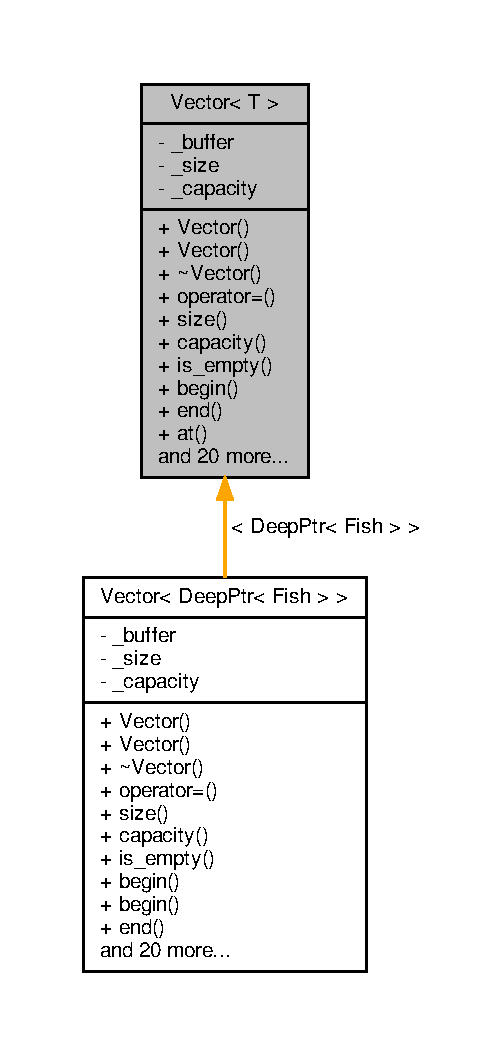
\includegraphics[width=242pt]{classVector__inherit__graph}
\end{center}
\end{figure}


Collaboration diagram for Vector$<$ T $>$\+:\nopagebreak
\begin{figure}[H]
\begin{center}
\leavevmode
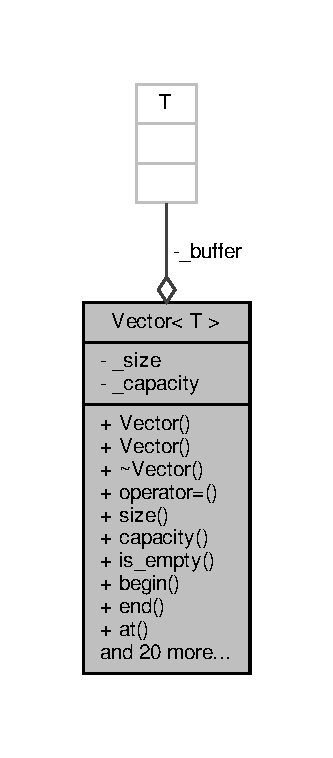
\includegraphics[width=160pt]{classVector__coll__graph}
\end{center}
\end{figure}
\subsection*{Classes}
\begin{DoxyCompactItemize}
\item 
class \hyperlink{classVector_1_1const__iterator}{const\+\_\+iterator}
\item 
class \hyperlink{classVector_1_1iterator}{iterator}
\end{DoxyCompactItemize}
\subsection*{Public Member Functions}
\begin{DoxyCompactItemize}
\item 
\hyperlink{classVector_aed1b9a621d7d2fc968e6e113fcda3f9a_aed1b9a621d7d2fc968e6e113fcda3f9a}{Vector} (unsigned int=0)
\item 
\hyperlink{classVector_a4edc1cac2c4cd6d3791280edabd89029_a4edc1cac2c4cd6d3791280edabd89029}{Vector} (const \hyperlink{classVector}{Vector} \&)
\item 
\hyperlink{classVector_afd524fac19e6d3d69db5198ffe2952b0_afd524fac19e6d3d69db5198ffe2952b0}{$\sim$\+Vector} ()
\item 
\hyperlink{classVector}{Vector} \& \hyperlink{classVector_a8d6906176604f2201919991acf655d13_a8d6906176604f2201919991acf655d13}{operator=} (const \hyperlink{classVector}{Vector} \&)
\item 
unsigned int \hyperlink{classVector_a5214a382564aedc712b609416aa3b7b1_a5214a382564aedc712b609416aa3b7b1}{size} () const
\item 
unsigned int \hyperlink{classVector_a68ecb8dc5e1047cead715396d146ed61_a68ecb8dc5e1047cead715396d146ed61}{capacity} () const
\item 
bool \hyperlink{classVector_a03a683aee83b3e9e0369a9e431a9259b_a03a683aee83b3e9e0369a9e431a9259b}{is\+\_\+empty} () const
\item 
\hyperlink{classVector_1_1iterator}{iterator} \hyperlink{classVector_ad1dc835efbf1859b3bd960c9b4f55ad4_ad1dc835efbf1859b3bd960c9b4f55ad4}{begin} ()
\item 
\hyperlink{classVector_1_1iterator}{iterator} \hyperlink{classVector_ac03563dbb2d417a36096b524a4875674_ac03563dbb2d417a36096b524a4875674}{end} ()
\item 
T \& \hyperlink{classVector_a3ae75814fa1b993c0abfd82aa513b5b3_a3ae75814fa1b993c0abfd82aa513b5b3}{at} (unsigned int)
\item 
T \& \hyperlink{classVector_a8b133b35c069989a02ed3db7e78cae02_a8b133b35c069989a02ed3db7e78cae02}{operator\mbox{[}$\,$\mbox{]}} (unsigned int)
\item 
T \& \hyperlink{classVector_a0061cc9127a9cbf541439121998a1fdd_a0061cc9127a9cbf541439121998a1fdd}{front} ()
\item 
T \& \hyperlink{classVector_a6decf0bdeb6849bfcc151b2c514f639f_a6decf0bdeb6849bfcc151b2c514f639f}{back} ()
\item 
\hyperlink{classVector_1_1const__iterator}{const\+\_\+iterator} \hyperlink{classVector_af8559abeb71f43efc0fc2933b79c3901_af8559abeb71f43efc0fc2933b79c3901}{begin} () const
\item 
\hyperlink{classVector_1_1const__iterator}{const\+\_\+iterator} \hyperlink{classVector_acb239aab833edfd7bb5ccd21c02ab505_acb239aab833edfd7bb5ccd21c02ab505}{end} () const
\item 
const T \& \hyperlink{classVector_a6287b84b91705e9caf0f3f197cc7e041_a6287b84b91705e9caf0f3f197cc7e041}{at} (unsigned int) const
\item 
const T \& \hyperlink{classVector_acf16259cd87643c68adfa44a0ff44eee_acf16259cd87643c68adfa44a0ff44eee}{operator\mbox{[}$\,$\mbox{]}} (unsigned int) const
\item 
const T \& \hyperlink{classVector_ae891494a5654af2db2a00d162c50985a_ae891494a5654af2db2a00d162c50985a}{front} () const
\item 
const T \& \hyperlink{classVector_ae2094e298cbe0394557b9213942a31d1_ae2094e298cbe0394557b9213942a31d1}{back} () const
\item 
void \hyperlink{classVector_a3c2e4666a28b07791817cc9562052732_a3c2e4666a28b07791817cc9562052732}{push\+\_\+back} (const T \&)
\item 
void \hyperlink{classVector_adcba035109febbe55cba2a25f8483ba6_adcba035109febbe55cba2a25f8483ba6}{pop\+\_\+back} ()
\item 
\hyperlink{classVector_1_1iterator}{iterator} \hyperlink{classVector_a423c0d0a3a93438489f596333e43990b_a423c0d0a3a93438489f596333e43990b}{erase} (\hyperlink{classVector_1_1iterator}{iterator})
\item 
void \hyperlink{classVector_a32ad98b135472b0ebc5d6cb3ae5d0085_a32ad98b135472b0ebc5d6cb3ae5d0085}{clear} ()
\item 
void \hyperlink{classVector_af3615fa3557b68d0e65f8c5519d51a8d_af3615fa3557b68d0e65f8c5519d51a8d}{reserve} (unsigned int)
\item 
void \hyperlink{classVector_addc1810308998ea4ecb85157edf8f023_addc1810308998ea4ecb85157edf8f023}{insert} (\hyperlink{classVector_1_1iterator}{iterator} pos, const T \&val)
\item 
void \hyperlink{classVector_ae4295ecbebe91ddef92c0e0d67f5be68_ae4295ecbebe91ddef92c0e0d67f5be68}{insert} (\hyperlink{classVector_1_1iterator}{iterator} pos, unsigned int fill, const T \&val)
\item 
void \hyperlink{classVector_a8000ae0fa6fb99c008b04fa7b07e40a1_a8000ae0fa6fb99c008b04fa7b07e40a1}{swap} (\hyperlink{classVector}{Vector} \&)
\item 
void \hyperlink{classVector_a2a6df7ae78537f9b0fe01ab7fc7cf442_a2a6df7ae78537f9b0fe01ab7fc7cf442}{resize} (unsigned int)
\item 
void \hyperlink{classVector_a76d7357d2ea8d1efc8de81b5e9efb95b_a76d7357d2ea8d1efc8de81b5e9efb95b}{resize} (unsigned int, const T \&)
\item 
void \hyperlink{classVector_ad6454ce193263b8000d4c18cb0c3a0c8_ad6454ce193263b8000d4c18cb0c3a0c8}{shrink\+\_\+to\+\_\+fit} ()
\end{DoxyCompactItemize}
\subsection*{Private Attributes}
\begin{DoxyCompactItemize}
\item 
T $\ast$ \hyperlink{classVector_a558d102b492fda3e325fddd1eb1b0266_a558d102b492fda3e325fddd1eb1b0266}{\+\_\+buffer}
\item 
unsigned int \hyperlink{classVector_acb6320b3ff4bf32733fbf0c279d8f895_acb6320b3ff4bf32733fbf0c279d8f895}{\+\_\+size}
\item 
unsigned int \hyperlink{classVector_a0c81b0e0d635e46bb65f05c6f12e08e8_a0c81b0e0d635e46bb65f05c6f12e08e8}{\+\_\+capacity}
\end{DoxyCompactItemize}


\subsection{Constructor \& Destructor Documentation}
\mbox{\Hypertarget{classVector_aed1b9a621d7d2fc968e6e113fcda3f9a_aed1b9a621d7d2fc968e6e113fcda3f9a}\label{classVector_aed1b9a621d7d2fc968e6e113fcda3f9a_aed1b9a621d7d2fc968e6e113fcda3f9a}} 
\index{Vector@{Vector}!Vector@{Vector}}
\index{Vector@{Vector}!Vector@{Vector}}
\subsubsection{\texorpdfstring{Vector()}{Vector()}\hspace{0.1cm}{\footnotesize\ttfamily [1/2]}}
{\footnotesize\ttfamily template$<$class T $>$ \\
\hyperlink{classVector}{Vector}$<$ T $>$\+::\hyperlink{classVector}{Vector} (\begin{DoxyParamCaption}\item[{unsigned int}]{capacity = {\ttfamily 0} }\end{DoxyParamCaption})}

\mbox{\Hypertarget{classVector_a4edc1cac2c4cd6d3791280edabd89029_a4edc1cac2c4cd6d3791280edabd89029}\label{classVector_a4edc1cac2c4cd6d3791280edabd89029_a4edc1cac2c4cd6d3791280edabd89029}} 
\index{Vector@{Vector}!Vector@{Vector}}
\index{Vector@{Vector}!Vector@{Vector}}
\subsubsection{\texorpdfstring{Vector()}{Vector()}\hspace{0.1cm}{\footnotesize\ttfamily [2/2]}}
{\footnotesize\ttfamily template$<$class T $>$ \\
\hyperlink{classVector}{Vector}$<$ T $>$\+::\hyperlink{classVector}{Vector} (\begin{DoxyParamCaption}\item[{const \hyperlink{classVector}{Vector}$<$ T $>$ \&}]{v }\end{DoxyParamCaption})}

\mbox{\Hypertarget{classVector_afd524fac19e6d3d69db5198ffe2952b0_afd524fac19e6d3d69db5198ffe2952b0}\label{classVector_afd524fac19e6d3d69db5198ffe2952b0_afd524fac19e6d3d69db5198ffe2952b0}} 
\index{Vector@{Vector}!````~Vector@{$\sim$\+Vector}}
\index{````~Vector@{$\sim$\+Vector}!Vector@{Vector}}
\subsubsection{\texorpdfstring{$\sim$\+Vector()}{~Vector()}}
{\footnotesize\ttfamily template$<$class T $>$ \\
\hyperlink{classVector}{Vector}$<$ T $>$\+::$\sim$\hyperlink{classVector}{Vector} (\begin{DoxyParamCaption}{ }\end{DoxyParamCaption})}



\subsection{Member Function Documentation}
\mbox{\Hypertarget{classVector_a3ae75814fa1b993c0abfd82aa513b5b3_a3ae75814fa1b993c0abfd82aa513b5b3}\label{classVector_a3ae75814fa1b993c0abfd82aa513b5b3_a3ae75814fa1b993c0abfd82aa513b5b3}} 
\index{Vector@{Vector}!at@{at}}
\index{at@{at}!Vector@{Vector}}
\subsubsection{\texorpdfstring{at()}{at()}\hspace{0.1cm}{\footnotesize\ttfamily [1/2]}}
{\footnotesize\ttfamily template$<$class T $>$ \\
T \& \hyperlink{classVector}{Vector}$<$ T $>$\+::at (\begin{DoxyParamCaption}\item[{unsigned int}]{index }\end{DoxyParamCaption})}

\mbox{\Hypertarget{classVector_a6287b84b91705e9caf0f3f197cc7e041_a6287b84b91705e9caf0f3f197cc7e041}\label{classVector_a6287b84b91705e9caf0f3f197cc7e041_a6287b84b91705e9caf0f3f197cc7e041}} 
\index{Vector@{Vector}!at@{at}}
\index{at@{at}!Vector@{Vector}}
\subsubsection{\texorpdfstring{at()}{at()}\hspace{0.1cm}{\footnotesize\ttfamily [2/2]}}
{\footnotesize\ttfamily template$<$class T $>$ \\
const T \& \hyperlink{classVector}{Vector}$<$ T $>$\+::at (\begin{DoxyParamCaption}\item[{unsigned int}]{index }\end{DoxyParamCaption}) const}

\mbox{\Hypertarget{classVector_a6decf0bdeb6849bfcc151b2c514f639f_a6decf0bdeb6849bfcc151b2c514f639f}\label{classVector_a6decf0bdeb6849bfcc151b2c514f639f_a6decf0bdeb6849bfcc151b2c514f639f}} 
\index{Vector@{Vector}!back@{back}}
\index{back@{back}!Vector@{Vector}}
\subsubsection{\texorpdfstring{back()}{back()}\hspace{0.1cm}{\footnotesize\ttfamily [1/2]}}
{\footnotesize\ttfamily template$<$class T $>$ \\
T \& \hyperlink{classVector}{Vector}$<$ T $>$\+::back (\begin{DoxyParamCaption}{ }\end{DoxyParamCaption})}

\mbox{\Hypertarget{classVector_ae2094e298cbe0394557b9213942a31d1_ae2094e298cbe0394557b9213942a31d1}\label{classVector_ae2094e298cbe0394557b9213942a31d1_ae2094e298cbe0394557b9213942a31d1}} 
\index{Vector@{Vector}!back@{back}}
\index{back@{back}!Vector@{Vector}}
\subsubsection{\texorpdfstring{back()}{back()}\hspace{0.1cm}{\footnotesize\ttfamily [2/2]}}
{\footnotesize\ttfamily template$<$class T $>$ \\
const T \& \hyperlink{classVector}{Vector}$<$ T $>$\+::back (\begin{DoxyParamCaption}{ }\end{DoxyParamCaption}) const}

\mbox{\Hypertarget{classVector_ad1dc835efbf1859b3bd960c9b4f55ad4_ad1dc835efbf1859b3bd960c9b4f55ad4}\label{classVector_ad1dc835efbf1859b3bd960c9b4f55ad4_ad1dc835efbf1859b3bd960c9b4f55ad4}} 
\index{Vector@{Vector}!begin@{begin}}
\index{begin@{begin}!Vector@{Vector}}
\subsubsection{\texorpdfstring{begin()}{begin()}\hspace{0.1cm}{\footnotesize\ttfamily [1/2]}}
{\footnotesize\ttfamily template$<$class T $>$ \\
\hyperlink{classVector}{Vector}$<$ T $>$\+::\hyperlink{classVector_1_1iterator}{iterator} \hyperlink{classVector}{Vector}$<$ T $>$\+::begin (\begin{DoxyParamCaption}{ }\end{DoxyParamCaption})}

\mbox{\Hypertarget{classVector_af8559abeb71f43efc0fc2933b79c3901_af8559abeb71f43efc0fc2933b79c3901}\label{classVector_af8559abeb71f43efc0fc2933b79c3901_af8559abeb71f43efc0fc2933b79c3901}} 
\index{Vector@{Vector}!begin@{begin}}
\index{begin@{begin}!Vector@{Vector}}
\subsubsection{\texorpdfstring{begin()}{begin()}\hspace{0.1cm}{\footnotesize\ttfamily [2/2]}}
{\footnotesize\ttfamily template$<$class T $>$ \\
\hyperlink{classVector}{Vector}$<$ T $>$\+::\hyperlink{classVector_1_1const__iterator}{const\+\_\+iterator} \hyperlink{classVector}{Vector}$<$ T $>$\+::begin (\begin{DoxyParamCaption}{ }\end{DoxyParamCaption}) const}

\mbox{\Hypertarget{classVector_a68ecb8dc5e1047cead715396d146ed61_a68ecb8dc5e1047cead715396d146ed61}\label{classVector_a68ecb8dc5e1047cead715396d146ed61_a68ecb8dc5e1047cead715396d146ed61}} 
\index{Vector@{Vector}!capacity@{capacity}}
\index{capacity@{capacity}!Vector@{Vector}}
\subsubsection{\texorpdfstring{capacity()}{capacity()}}
{\footnotesize\ttfamily template$<$class T $>$ \\
unsigned int \hyperlink{classVector}{Vector}$<$ T $>$\+::capacity (\begin{DoxyParamCaption}{ }\end{DoxyParamCaption}) const}

\mbox{\Hypertarget{classVector_a32ad98b135472b0ebc5d6cb3ae5d0085_a32ad98b135472b0ebc5d6cb3ae5d0085}\label{classVector_a32ad98b135472b0ebc5d6cb3ae5d0085_a32ad98b135472b0ebc5d6cb3ae5d0085}} 
\index{Vector@{Vector}!clear@{clear}}
\index{clear@{clear}!Vector@{Vector}}
\subsubsection{\texorpdfstring{clear()}{clear()}}
{\footnotesize\ttfamily template$<$class T $>$ \\
void \hyperlink{classVector}{Vector}$<$ T $>$\+::clear (\begin{DoxyParamCaption}{ }\end{DoxyParamCaption})}

\mbox{\Hypertarget{classVector_ac03563dbb2d417a36096b524a4875674_ac03563dbb2d417a36096b524a4875674}\label{classVector_ac03563dbb2d417a36096b524a4875674_ac03563dbb2d417a36096b524a4875674}} 
\index{Vector@{Vector}!end@{end}}
\index{end@{end}!Vector@{Vector}}
\subsubsection{\texorpdfstring{end()}{end()}\hspace{0.1cm}{\footnotesize\ttfamily [1/2]}}
{\footnotesize\ttfamily template$<$class T $>$ \\
\hyperlink{classVector}{Vector}$<$ T $>$\+::\hyperlink{classVector_1_1iterator}{iterator} \hyperlink{classVector}{Vector}$<$ T $>$\+::end (\begin{DoxyParamCaption}{ }\end{DoxyParamCaption})}

\mbox{\Hypertarget{classVector_acb239aab833edfd7bb5ccd21c02ab505_acb239aab833edfd7bb5ccd21c02ab505}\label{classVector_acb239aab833edfd7bb5ccd21c02ab505_acb239aab833edfd7bb5ccd21c02ab505}} 
\index{Vector@{Vector}!end@{end}}
\index{end@{end}!Vector@{Vector}}
\subsubsection{\texorpdfstring{end()}{end()}\hspace{0.1cm}{\footnotesize\ttfamily [2/2]}}
{\footnotesize\ttfamily template$<$class T $>$ \\
\hyperlink{classVector}{Vector}$<$ T $>$\+::\hyperlink{classVector_1_1const__iterator}{const\+\_\+iterator} \hyperlink{classVector}{Vector}$<$ T $>$\+::end (\begin{DoxyParamCaption}{ }\end{DoxyParamCaption}) const}

\mbox{\Hypertarget{classVector_a423c0d0a3a93438489f596333e43990b_a423c0d0a3a93438489f596333e43990b}\label{classVector_a423c0d0a3a93438489f596333e43990b_a423c0d0a3a93438489f596333e43990b}} 
\index{Vector@{Vector}!erase@{erase}}
\index{erase@{erase}!Vector@{Vector}}
\subsubsection{\texorpdfstring{erase()}{erase()}}
{\footnotesize\ttfamily template$<$class T$>$ \\
\hyperlink{classVector}{Vector}$<$ T $>$\+::\hyperlink{classVector_1_1iterator}{iterator} \hyperlink{classVector}{Vector}$<$ T $>$\+::erase (\begin{DoxyParamCaption}\item[{\hyperlink{classVector_1_1iterator}{iterator}}]{ }\end{DoxyParamCaption})}

\mbox{\Hypertarget{classVector_a0061cc9127a9cbf541439121998a1fdd_a0061cc9127a9cbf541439121998a1fdd}\label{classVector_a0061cc9127a9cbf541439121998a1fdd_a0061cc9127a9cbf541439121998a1fdd}} 
\index{Vector@{Vector}!front@{front}}
\index{front@{front}!Vector@{Vector}}
\subsubsection{\texorpdfstring{front()}{front()}\hspace{0.1cm}{\footnotesize\ttfamily [1/2]}}
{\footnotesize\ttfamily template$<$class T $>$ \\
T \& \hyperlink{classVector}{Vector}$<$ T $>$\+::front (\begin{DoxyParamCaption}{ }\end{DoxyParamCaption})}

\mbox{\Hypertarget{classVector_ae891494a5654af2db2a00d162c50985a_ae891494a5654af2db2a00d162c50985a}\label{classVector_ae891494a5654af2db2a00d162c50985a_ae891494a5654af2db2a00d162c50985a}} 
\index{Vector@{Vector}!front@{front}}
\index{front@{front}!Vector@{Vector}}
\subsubsection{\texorpdfstring{front()}{front()}\hspace{0.1cm}{\footnotesize\ttfamily [2/2]}}
{\footnotesize\ttfamily template$<$class T $>$ \\
const T \& \hyperlink{classVector}{Vector}$<$ T $>$\+::front (\begin{DoxyParamCaption}{ }\end{DoxyParamCaption}) const}

\mbox{\Hypertarget{classVector_addc1810308998ea4ecb85157edf8f023_addc1810308998ea4ecb85157edf8f023}\label{classVector_addc1810308998ea4ecb85157edf8f023_addc1810308998ea4ecb85157edf8f023}} 
\index{Vector@{Vector}!insert@{insert}}
\index{insert@{insert}!Vector@{Vector}}
\subsubsection{\texorpdfstring{insert()}{insert()}\hspace{0.1cm}{\footnotesize\ttfamily [1/2]}}
{\footnotesize\ttfamily template$<$class T$>$ \\
void \hyperlink{classVector}{Vector}$<$ T $>$\+::insert (\begin{DoxyParamCaption}\item[{\hyperlink{classVector_1_1iterator}{iterator}}]{pos,  }\item[{const T \&}]{val }\end{DoxyParamCaption})}

\mbox{\Hypertarget{classVector_ae4295ecbebe91ddef92c0e0d67f5be68_ae4295ecbebe91ddef92c0e0d67f5be68}\label{classVector_ae4295ecbebe91ddef92c0e0d67f5be68_ae4295ecbebe91ddef92c0e0d67f5be68}} 
\index{Vector@{Vector}!insert@{insert}}
\index{insert@{insert}!Vector@{Vector}}
\subsubsection{\texorpdfstring{insert()}{insert()}\hspace{0.1cm}{\footnotesize\ttfamily [2/2]}}
{\footnotesize\ttfamily template$<$class T$>$ \\
void \hyperlink{classVector}{Vector}$<$ T $>$\+::insert (\begin{DoxyParamCaption}\item[{\hyperlink{classVector_1_1iterator}{iterator}}]{pos,  }\item[{unsigned int}]{fill,  }\item[{const T \&}]{val }\end{DoxyParamCaption})}

\mbox{\Hypertarget{classVector_a03a683aee83b3e9e0369a9e431a9259b_a03a683aee83b3e9e0369a9e431a9259b}\label{classVector_a03a683aee83b3e9e0369a9e431a9259b_a03a683aee83b3e9e0369a9e431a9259b}} 
\index{Vector@{Vector}!is\+\_\+empty@{is\+\_\+empty}}
\index{is\+\_\+empty@{is\+\_\+empty}!Vector@{Vector}}
\subsubsection{\texorpdfstring{is\+\_\+empty()}{is\_empty()}}
{\footnotesize\ttfamily template$<$class T $>$ \\
bool \hyperlink{classVector}{Vector}$<$ T $>$\+::is\+\_\+empty (\begin{DoxyParamCaption}{ }\end{DoxyParamCaption}) const}

\mbox{\Hypertarget{classVector_a8d6906176604f2201919991acf655d13_a8d6906176604f2201919991acf655d13}\label{classVector_a8d6906176604f2201919991acf655d13_a8d6906176604f2201919991acf655d13}} 
\index{Vector@{Vector}!operator=@{operator=}}
\index{operator=@{operator=}!Vector@{Vector}}
\subsubsection{\texorpdfstring{operator=()}{operator=()}}
{\footnotesize\ttfamily template$<$class T $>$ \\
\hyperlink{classVector}{Vector}$<$ T $>$ \& \hyperlink{classVector}{Vector}$<$ T $>$\+::operator= (\begin{DoxyParamCaption}\item[{const \hyperlink{classVector}{Vector}$<$ T $>$ \&}]{v }\end{DoxyParamCaption})}

\mbox{\Hypertarget{classVector_a8b133b35c069989a02ed3db7e78cae02_a8b133b35c069989a02ed3db7e78cae02}\label{classVector_a8b133b35c069989a02ed3db7e78cae02_a8b133b35c069989a02ed3db7e78cae02}} 
\index{Vector@{Vector}!operator\mbox{[}\mbox{]}@{operator[]}}
\index{operator\mbox{[}\mbox{]}@{operator[]}!Vector@{Vector}}
\subsubsection{\texorpdfstring{operator[]()}{operator[]()}\hspace{0.1cm}{\footnotesize\ttfamily [1/2]}}
{\footnotesize\ttfamily template$<$class T $>$ \\
T \& \hyperlink{classVector}{Vector}$<$ T $>$\+::operator\mbox{[}$\,$\mbox{]} (\begin{DoxyParamCaption}\item[{unsigned int}]{index }\end{DoxyParamCaption})}

\mbox{\Hypertarget{classVector_acf16259cd87643c68adfa44a0ff44eee_acf16259cd87643c68adfa44a0ff44eee}\label{classVector_acf16259cd87643c68adfa44a0ff44eee_acf16259cd87643c68adfa44a0ff44eee}} 
\index{Vector@{Vector}!operator\mbox{[}\mbox{]}@{operator[]}}
\index{operator\mbox{[}\mbox{]}@{operator[]}!Vector@{Vector}}
\subsubsection{\texorpdfstring{operator[]()}{operator[]()}\hspace{0.1cm}{\footnotesize\ttfamily [2/2]}}
{\footnotesize\ttfamily template$<$class T $>$ \\
const T \& \hyperlink{classVector}{Vector}$<$ T $>$\+::operator\mbox{[}$\,$\mbox{]} (\begin{DoxyParamCaption}\item[{unsigned int}]{index }\end{DoxyParamCaption}) const}

\mbox{\Hypertarget{classVector_adcba035109febbe55cba2a25f8483ba6_adcba035109febbe55cba2a25f8483ba6}\label{classVector_adcba035109febbe55cba2a25f8483ba6_adcba035109febbe55cba2a25f8483ba6}} 
\index{Vector@{Vector}!pop\+\_\+back@{pop\+\_\+back}}
\index{pop\+\_\+back@{pop\+\_\+back}!Vector@{Vector}}
\subsubsection{\texorpdfstring{pop\+\_\+back()}{pop\_back()}}
{\footnotesize\ttfamily template$<$class T $>$ \\
void \hyperlink{classVector}{Vector}$<$ T $>$\+::pop\+\_\+back (\begin{DoxyParamCaption}{ }\end{DoxyParamCaption})}

\mbox{\Hypertarget{classVector_a3c2e4666a28b07791817cc9562052732_a3c2e4666a28b07791817cc9562052732}\label{classVector_a3c2e4666a28b07791817cc9562052732_a3c2e4666a28b07791817cc9562052732}} 
\index{Vector@{Vector}!push\+\_\+back@{push\+\_\+back}}
\index{push\+\_\+back@{push\+\_\+back}!Vector@{Vector}}
\subsubsection{\texorpdfstring{push\+\_\+back()}{push\_back()}}
{\footnotesize\ttfamily template$<$class T$>$ \\
void \hyperlink{classVector}{Vector}$<$ T $>$\+::push\+\_\+back (\begin{DoxyParamCaption}\item[{const T \&}]{v }\end{DoxyParamCaption})}

\mbox{\Hypertarget{classVector_af3615fa3557b68d0e65f8c5519d51a8d_af3615fa3557b68d0e65f8c5519d51a8d}\label{classVector_af3615fa3557b68d0e65f8c5519d51a8d_af3615fa3557b68d0e65f8c5519d51a8d}} 
\index{Vector@{Vector}!reserve@{reserve}}
\index{reserve@{reserve}!Vector@{Vector}}
\subsubsection{\texorpdfstring{reserve()}{reserve()}}
{\footnotesize\ttfamily template$<$class T $>$ \\
void \hyperlink{classVector}{Vector}$<$ T $>$\+::reserve (\begin{DoxyParamCaption}\item[{unsigned int}]{n }\end{DoxyParamCaption})}

\mbox{\Hypertarget{classVector_a2a6df7ae78537f9b0fe01ab7fc7cf442_a2a6df7ae78537f9b0fe01ab7fc7cf442}\label{classVector_a2a6df7ae78537f9b0fe01ab7fc7cf442_a2a6df7ae78537f9b0fe01ab7fc7cf442}} 
\index{Vector@{Vector}!resize@{resize}}
\index{resize@{resize}!Vector@{Vector}}
\subsubsection{\texorpdfstring{resize()}{resize()}\hspace{0.1cm}{\footnotesize\ttfamily [1/2]}}
{\footnotesize\ttfamily template$<$class T $>$ \\
void \hyperlink{classVector}{Vector}$<$ T $>$\+::resize (\begin{DoxyParamCaption}\item[{unsigned int}]{newsize }\end{DoxyParamCaption})}

\mbox{\Hypertarget{classVector_a76d7357d2ea8d1efc8de81b5e9efb95b_a76d7357d2ea8d1efc8de81b5e9efb95b}\label{classVector_a76d7357d2ea8d1efc8de81b5e9efb95b_a76d7357d2ea8d1efc8de81b5e9efb95b}} 
\index{Vector@{Vector}!resize@{resize}}
\index{resize@{resize}!Vector@{Vector}}
\subsubsection{\texorpdfstring{resize()}{resize()}\hspace{0.1cm}{\footnotesize\ttfamily [2/2]}}
{\footnotesize\ttfamily template$<$class T$>$ \\
void \hyperlink{classVector}{Vector}$<$ T $>$\+::resize (\begin{DoxyParamCaption}\item[{unsigned int}]{newsize,  }\item[{const T \&}]{v }\end{DoxyParamCaption})}

\mbox{\Hypertarget{classVector_ad6454ce193263b8000d4c18cb0c3a0c8_ad6454ce193263b8000d4c18cb0c3a0c8}\label{classVector_ad6454ce193263b8000d4c18cb0c3a0c8_ad6454ce193263b8000d4c18cb0c3a0c8}} 
\index{Vector@{Vector}!shrink\+\_\+to\+\_\+fit@{shrink\+\_\+to\+\_\+fit}}
\index{shrink\+\_\+to\+\_\+fit@{shrink\+\_\+to\+\_\+fit}!Vector@{Vector}}
\subsubsection{\texorpdfstring{shrink\+\_\+to\+\_\+fit()}{shrink\_to\_fit()}}
{\footnotesize\ttfamily template$<$class T $>$ \\
void \hyperlink{classVector}{Vector}$<$ T $>$\+::shrink\+\_\+to\+\_\+fit (\begin{DoxyParamCaption}{ }\end{DoxyParamCaption})}

\mbox{\Hypertarget{classVector_a5214a382564aedc712b609416aa3b7b1_a5214a382564aedc712b609416aa3b7b1}\label{classVector_a5214a382564aedc712b609416aa3b7b1_a5214a382564aedc712b609416aa3b7b1}} 
\index{Vector@{Vector}!size@{size}}
\index{size@{size}!Vector@{Vector}}
\subsubsection{\texorpdfstring{size()}{size()}}
{\footnotesize\ttfamily template$<$class T $>$ \\
unsigned int \hyperlink{classVector}{Vector}$<$ T $>$\+::size (\begin{DoxyParamCaption}{ }\end{DoxyParamCaption}) const}

\mbox{\Hypertarget{classVector_a8000ae0fa6fb99c008b04fa7b07e40a1_a8000ae0fa6fb99c008b04fa7b07e40a1}\label{classVector_a8000ae0fa6fb99c008b04fa7b07e40a1_a8000ae0fa6fb99c008b04fa7b07e40a1}} 
\index{Vector@{Vector}!swap@{swap}}
\index{swap@{swap}!Vector@{Vector}}
\subsubsection{\texorpdfstring{swap()}{swap()}}
{\footnotesize\ttfamily template$<$class T$>$ \\
void \hyperlink{classVector}{Vector}$<$ T $>$\+::swap (\begin{DoxyParamCaption}\item[{\hyperlink{classVector}{Vector}$<$ T $>$ \&}]{ }\end{DoxyParamCaption})}



\subsection{Member Data Documentation}
\mbox{\Hypertarget{classVector_a558d102b492fda3e325fddd1eb1b0266_a558d102b492fda3e325fddd1eb1b0266}\label{classVector_a558d102b492fda3e325fddd1eb1b0266_a558d102b492fda3e325fddd1eb1b0266}} 
\index{Vector@{Vector}!\+\_\+buffer@{\+\_\+buffer}}
\index{\+\_\+buffer@{\+\_\+buffer}!Vector@{Vector}}
\subsubsection{\texorpdfstring{\+\_\+buffer}{\_buffer}}
{\footnotesize\ttfamily template$<$class T$>$ \\
T$\ast$ \hyperlink{classVector}{Vector}$<$ T $>$\+::\+\_\+buffer\hspace{0.3cm}{\ttfamily [private]}}

\mbox{\Hypertarget{classVector_a0c81b0e0d635e46bb65f05c6f12e08e8_a0c81b0e0d635e46bb65f05c6f12e08e8}\label{classVector_a0c81b0e0d635e46bb65f05c6f12e08e8_a0c81b0e0d635e46bb65f05c6f12e08e8}} 
\index{Vector@{Vector}!\+\_\+capacity@{\+\_\+capacity}}
\index{\+\_\+capacity@{\+\_\+capacity}!Vector@{Vector}}
\subsubsection{\texorpdfstring{\+\_\+capacity}{\_capacity}}
{\footnotesize\ttfamily template$<$class T$>$ \\
unsigned int \hyperlink{classVector}{Vector}$<$ T $>$\+::\+\_\+capacity\hspace{0.3cm}{\ttfamily [private]}}

\mbox{\Hypertarget{classVector_acb6320b3ff4bf32733fbf0c279d8f895_acb6320b3ff4bf32733fbf0c279d8f895}\label{classVector_acb6320b3ff4bf32733fbf0c279d8f895_acb6320b3ff4bf32733fbf0c279d8f895}} 
\index{Vector@{Vector}!\+\_\+size@{\+\_\+size}}
\index{\+\_\+size@{\+\_\+size}!Vector@{Vector}}
\subsubsection{\texorpdfstring{\+\_\+size}{\_size}}
{\footnotesize\ttfamily template$<$class T$>$ \\
unsigned int \hyperlink{classVector}{Vector}$<$ T $>$\+::\+\_\+size\hspace{0.3cm}{\ttfamily [private]}}



The documentation for this class was generated from the following file\+:\begin{DoxyCompactItemize}
\item 
include/\hyperlink{vector_8hpp}{vector.\+hpp}\end{DoxyCompactItemize}

\hypertarget{classVehicle}{}\section{Vehicle Class Reference}
\label{classVehicle}\index{Vehicle@{Vehicle}}


{\ttfamily \#include $<$vehicle.\+hpp$>$}



Inheritance diagram for Vehicle\+:\nopagebreak
\begin{figure}[H]
\begin{center}
\leavevmode
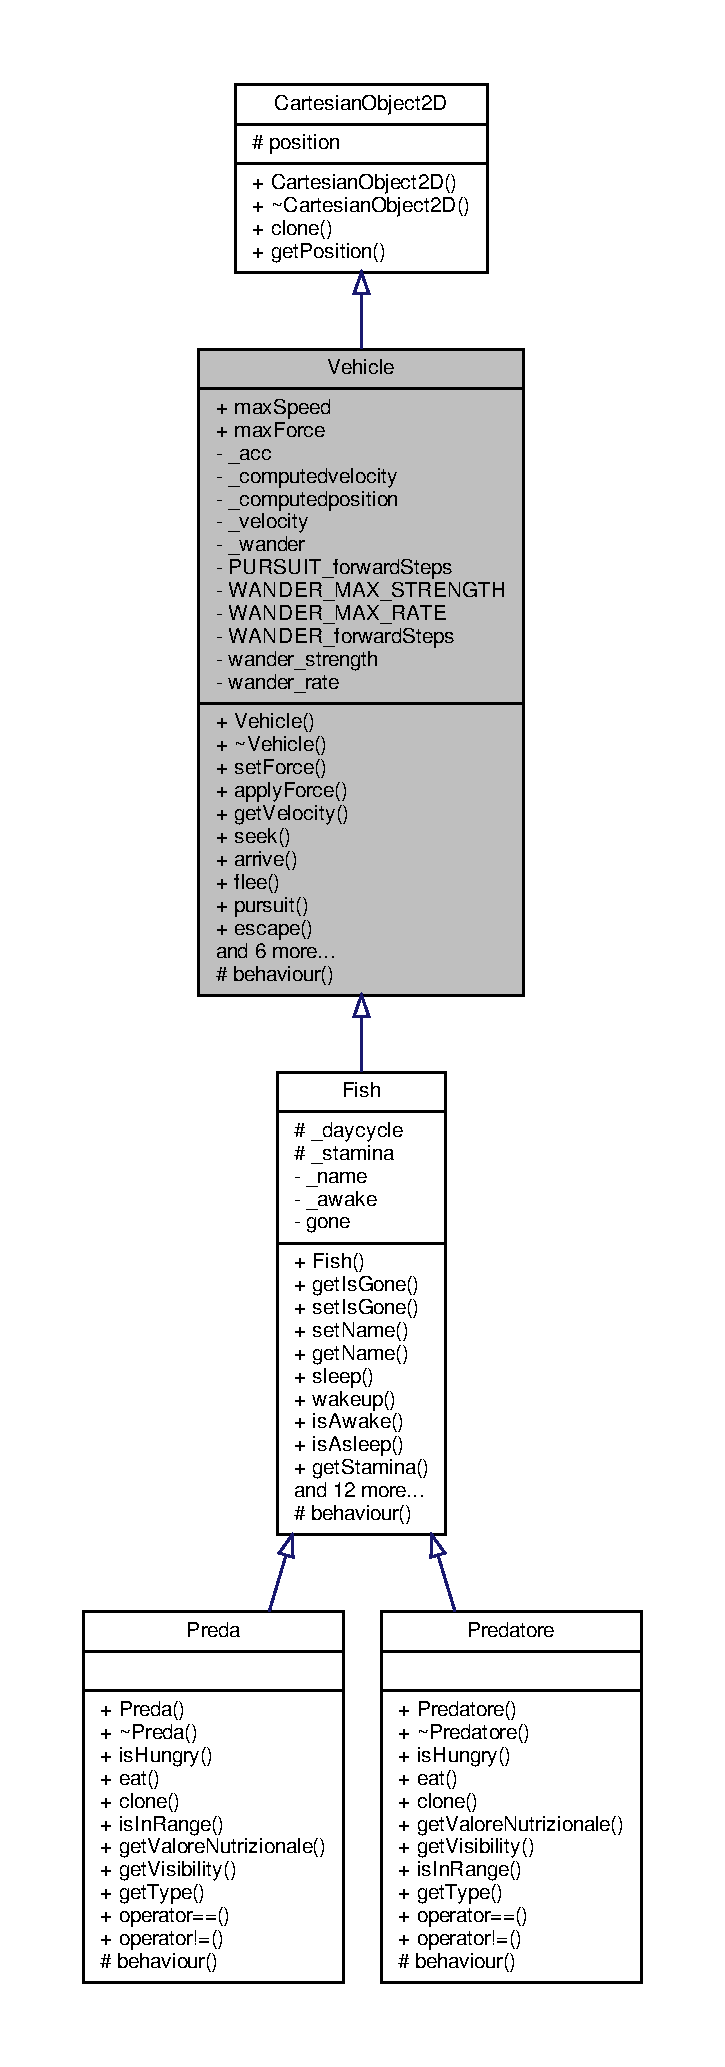
\includegraphics[height=550pt]{classVehicle__inherit__graph}
\end{center}
\end{figure}


Collaboration diagram for Vehicle\+:\nopagebreak
\begin{figure}[H]
\begin{center}
\leavevmode
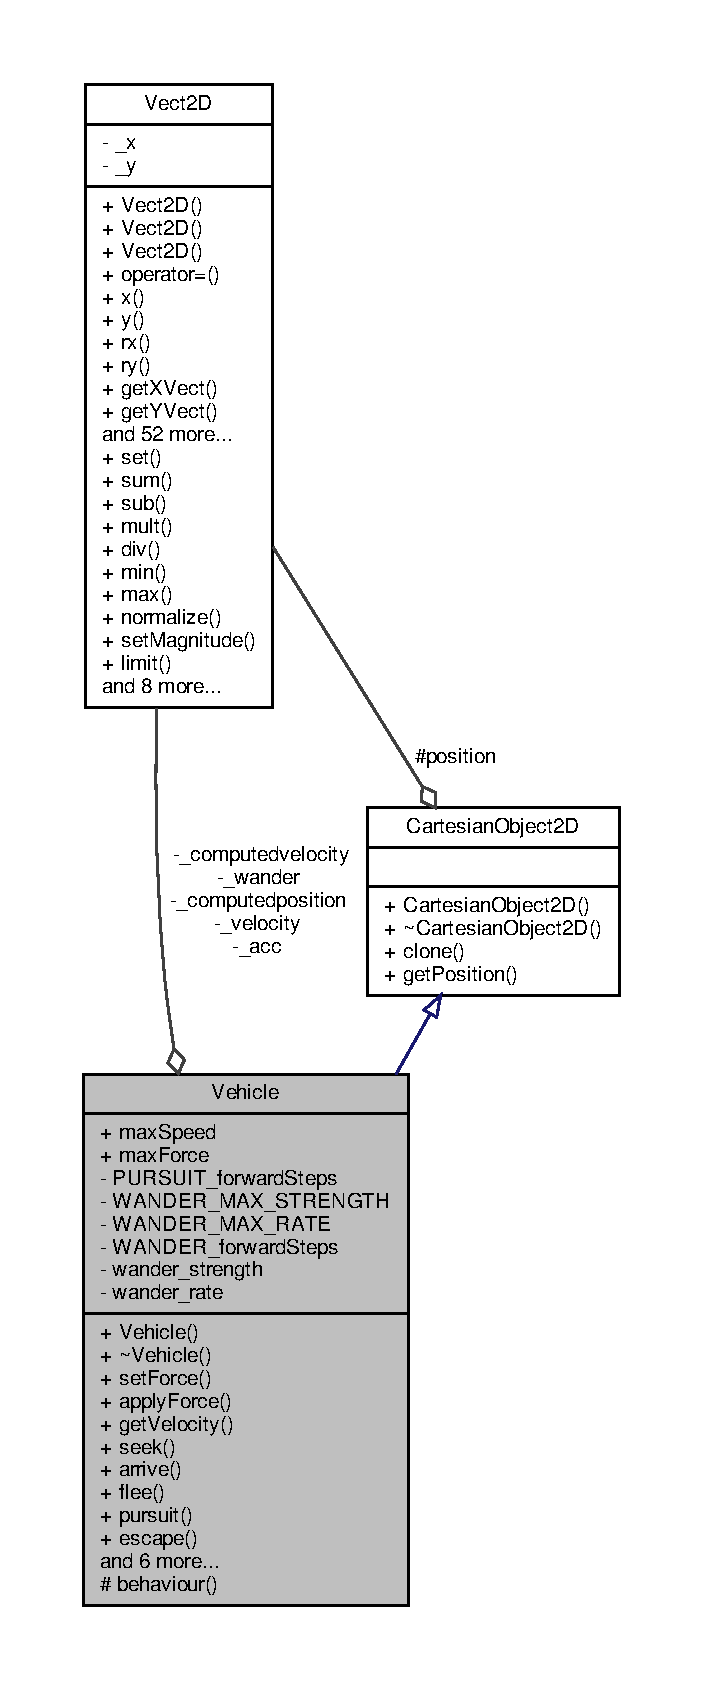
\includegraphics[height=550pt]{classVehicle__coll__graph}
\end{center}
\end{figure}
\subsection*{Public Member Functions}
\begin{DoxyCompactItemize}
\item 
\hyperlink{classVehicle_abaad8187d9f2ede4fb8ea18de0a6764c_abaad8187d9f2ede4fb8ea18de0a6764c}{Vehicle} ()
\item 
virtual \hyperlink{classVehicle_a61ab140c755b8e0e824d54117cf4546f_a61ab140c755b8e0e824d54117cf4546f}{$\sim$\+Vehicle} ()
\item 
void \hyperlink{classVehicle_a03e22c522e6f526f95428c81d0762833_a03e22c522e6f526f95428c81d0762833}{set\+Force} (const \hyperlink{classVect2D}{Vect2D} \&)
\item 
void \hyperlink{classVehicle_a82fbbd5aafc1ba89c3daa4da09989bbe_a82fbbd5aafc1ba89c3daa4da09989bbe}{apply\+Force} (const \hyperlink{classVect2D}{Vect2D} \&, const double \&=1)
\item 
const \hyperlink{classVect2D}{Vect2D} \& \hyperlink{classVehicle_a87b8266cb3495e8444233a0724e1bf07_a87b8266cb3495e8444233a0724e1bf07}{get\+Velocity} () const
\item 
\hyperlink{classVect2D}{Vect2D} \hyperlink{classVehicle_a86c0b5ddcf64443bc090657cd29832bf_a86c0b5ddcf64443bc090657cd29832bf}{seek} (const \hyperlink{classVect2D}{Vect2D} \&) const
\item 
\hyperlink{classVect2D}{Vect2D} \hyperlink{classVehicle_a55f8bb6cfbdd97219c2cea6cf3ad3826_a55f8bb6cfbdd97219c2cea6cf3ad3826}{arrive} (const \hyperlink{classVect2D}{Vect2D} \&) const
\item 
\hyperlink{classVect2D}{Vect2D} \hyperlink{classVehicle_ac7dbbb2942b8d642b2ab071def1c2fdb_ac7dbbb2942b8d642b2ab071def1c2fdb}{flee} (const \hyperlink{classVect2D}{Vect2D} \&) const
\item 
\hyperlink{classVect2D}{Vect2D} \hyperlink{classVehicle_a9dd4f4a06b4abd3324d317c27bb867d2_a9dd4f4a06b4abd3324d317c27bb867d2}{pursuit} (const \hyperlink{classVehicle}{Vehicle} \&) const
\item 
\hyperlink{classVect2D}{Vect2D} \hyperlink{classVehicle_ae5fbf395cbebf51498cbe8b2baaddc16_ae5fbf395cbebf51498cbe8b2baaddc16}{escape} (const \hyperlink{classVehicle}{Vehicle} \&) const
\item 
\hyperlink{classVect2D}{Vect2D} \hyperlink{classVehicle_af9da94116706c94e5f26df42c258dc6e_af9da94116706c94e5f26df42c258dc6e}{wander} ()
\item 
\hyperlink{classVect2D}{Vect2D} \hyperlink{classVehicle_a9a1cb1e5dab4a474fbe0c1c49482d0ee_a9a1cb1e5dab4a474fbe0c1c49482d0ee}{stop} () const
\item 
\hyperlink{classVect2D}{Vect2D} \hyperlink{classVehicle_a6149abf3e3f67df45d950562034d0fae_a6149abf3e3f67df45d950562034d0fae}{stay\+Within\+Borders} (const \hyperlink{classVect2D}{Vect2D} \&, const unsigned int distance) const
\item 
virtual \hyperlink{classVehicle}{Vehicle} $\ast$ \hyperlink{classVehicle_a6c8513134608499d188a2e994accdb7c_a6c8513134608499d188a2e994accdb7c}{clone} () const =0
\item 
virtual bool \hyperlink{classVehicle_a49a29a7ce993a33f78b96e7b368c60fd_a49a29a7ce993a33f78b96e7b368c60fd}{is\+In\+Range} (const \hyperlink{classVect2D}{Vect2D} \&v) const =0
\item 
virtual void \hyperlink{classVehicle_aa4ffd7e5fd11297950347de4e8b5ec93_aa4ffd7e5fd11297950347de4e8b5ec93}{advance} (\hyperlink{classAquarius}{Aquarius} $\ast$a, int phase) final
\item 
\hyperlink{classVect2D}{Vect2D} \hyperlink{classCartesianObject2D_aa3a6b63777852ab9eb9408ed2536abe2_aa3a6b63777852ab9eb9408ed2536abe2}{get\+Position} () const
\end{DoxyCompactItemize}
\subsection*{Static Public Attributes}
\begin{DoxyCompactItemize}
\item 
static const double \hyperlink{classVehicle_aab47c62e89baa5b7e52c2292451fbcb6_aab47c62e89baa5b7e52c2292451fbcb6}{max\+Speed} = 5
\item 
static const double \hyperlink{classVehicle_a95c56790e3dc52ab0fa54c279920be54_a95c56790e3dc52ab0fa54c279920be54}{max\+Force} = .\+15
\end{DoxyCompactItemize}
\subsection*{Protected Member Functions}
\begin{DoxyCompactItemize}
\item 
virtual void \hyperlink{classVehicle_a7b8b7578202a306a4dc08d587dc70f17_a7b8b7578202a306a4dc08d587dc70f17}{behaviour} (\hyperlink{classAquarius}{Aquarius} $\ast$)=0
\end{DoxyCompactItemize}
\subsection*{Protected Attributes}
\begin{DoxyCompactItemize}
\item 
\hyperlink{classVect2D}{Vect2D} \hyperlink{classCartesianObject2D_ae02ec6ed11f9bfc0c748da033d6a32f9_ae02ec6ed11f9bfc0c748da033d6a32f9}{position}
\end{DoxyCompactItemize}
\subsection*{Private Attributes}
\begin{DoxyCompactItemize}
\item 
\hyperlink{classVect2D}{Vect2D} \hyperlink{classVehicle_a6fbb45a38a758844f9a476ca720ba3f1_a6fbb45a38a758844f9a476ca720ba3f1}{\+\_\+acc}
\item 
\hyperlink{classVect2D}{Vect2D} \hyperlink{classVehicle_a6225fb68a1f2529e3f3c2d7bc47ae9e6_a6225fb68a1f2529e3f3c2d7bc47ae9e6}{\+\_\+computedvelocity}
\item 
\hyperlink{classVect2D}{Vect2D} \hyperlink{classVehicle_a81aa6e8ba6d8d1b6c6efa2d7736a5df4_a81aa6e8ba6d8d1b6c6efa2d7736a5df4}{\+\_\+computedposition}
\item 
\hyperlink{classVect2D}{Vect2D} \hyperlink{classVehicle_ac888ee5c6b81670f4cb376183b695b57_ac888ee5c6b81670f4cb376183b695b57}{\+\_\+velocity}
\item 
\hyperlink{classVect2D}{Vect2D} \hyperlink{classVehicle_ade0caf971a0a07f5ca3c50e67af95053_ade0caf971a0a07f5ca3c50e67af95053}{\+\_\+wander}
\end{DoxyCompactItemize}
\subsection*{Static Private Attributes}
\begin{DoxyCompactItemize}
\item 
static const double \hyperlink{classVehicle_a1767dabf75009d56e4f4e19712e27041_a1767dabf75009d56e4f4e19712e27041}{P\+U\+R\+S\+U\+I\+T\+\_\+forward\+Steps} = 5
\item 
static const double \hyperlink{classVehicle_a88e3c18986136f7724381cbb432b4b9e_a88e3c18986136f7724381cbb432b4b9e}{W\+A\+N\+D\+E\+R\+\_\+\+M\+A\+X\+\_\+\+S\+T\+R\+E\+N\+G\+TH} = 5
\item 
static const double \hyperlink{classVehicle_a1b8a65b38d64423f3face242225e32ff_a1b8a65b38d64423f3face242225e32ff}{W\+A\+N\+D\+E\+R\+\_\+\+M\+A\+X\+\_\+\+R\+A\+TE} = 20
\item 
static const double \hyperlink{classVehicle_af0cdca2c471fc2a8b1550901a87b6f33_af0cdca2c471fc2a8b1550901a87b6f33}{W\+A\+N\+D\+E\+R\+\_\+forward\+Steps} = 15
\item 
static const double \hyperlink{classVehicle_aa9821d59ca26c38cf6189695d92320a4_aa9821d59ca26c38cf6189695d92320a4}{wander\+\_\+strength} = 1
\item 
static const double \hyperlink{classVehicle_a2ac138ed3a9f59ccd31c04fa82cd3dfb_a2ac138ed3a9f59ccd31c04fa82cd3dfb}{wander\+\_\+rate} = 1
\end{DoxyCompactItemize}


\subsection{Constructor \& Destructor Documentation}
\mbox{\Hypertarget{classVehicle_abaad8187d9f2ede4fb8ea18de0a6764c_abaad8187d9f2ede4fb8ea18de0a6764c}\label{classVehicle_abaad8187d9f2ede4fb8ea18de0a6764c_abaad8187d9f2ede4fb8ea18de0a6764c}} 
\index{Vehicle@{Vehicle}!Vehicle@{Vehicle}}
\index{Vehicle@{Vehicle}!Vehicle@{Vehicle}}
\subsubsection{\texorpdfstring{Vehicle()}{Vehicle()}}
{\footnotesize\ttfamily Vehicle\+::\+Vehicle (\begin{DoxyParamCaption}{ }\end{DoxyParamCaption})}

\mbox{\Hypertarget{classVehicle_a61ab140c755b8e0e824d54117cf4546f_a61ab140c755b8e0e824d54117cf4546f}\label{classVehicle_a61ab140c755b8e0e824d54117cf4546f_a61ab140c755b8e0e824d54117cf4546f}} 
\index{Vehicle@{Vehicle}!````~Vehicle@{$\sim$\+Vehicle}}
\index{````~Vehicle@{$\sim$\+Vehicle}!Vehicle@{Vehicle}}
\subsubsection{\texorpdfstring{$\sim$\+Vehicle()}{~Vehicle()}}
{\footnotesize\ttfamily Vehicle\+::$\sim$\+Vehicle (\begin{DoxyParamCaption}{ }\end{DoxyParamCaption})\hspace{0.3cm}{\ttfamily [virtual]}, {\ttfamily [default]}}



\subsection{Member Function Documentation}
\mbox{\Hypertarget{classVehicle_aa4ffd7e5fd11297950347de4e8b5ec93_aa4ffd7e5fd11297950347de4e8b5ec93}\label{classVehicle_aa4ffd7e5fd11297950347de4e8b5ec93_aa4ffd7e5fd11297950347de4e8b5ec93}} 
\index{Vehicle@{Vehicle}!advance@{advance}}
\index{advance@{advance}!Vehicle@{Vehicle}}
\subsubsection{\texorpdfstring{advance()}{advance()}}
{\footnotesize\ttfamily void Vehicle\+::advance (\begin{DoxyParamCaption}\item[{\hyperlink{classAquarius}{Aquarius} $\ast$}]{a,  }\item[{int}]{phase }\end{DoxyParamCaption})\hspace{0.3cm}{\ttfamily [final]}, {\ttfamily [virtual]}}

\mbox{\Hypertarget{classVehicle_a82fbbd5aafc1ba89c3daa4da09989bbe_a82fbbd5aafc1ba89c3daa4da09989bbe}\label{classVehicle_a82fbbd5aafc1ba89c3daa4da09989bbe_a82fbbd5aafc1ba89c3daa4da09989bbe}} 
\index{Vehicle@{Vehicle}!apply\+Force@{apply\+Force}}
\index{apply\+Force@{apply\+Force}!Vehicle@{Vehicle}}
\subsubsection{\texorpdfstring{apply\+Force()}{applyForce()}}
{\footnotesize\ttfamily void Vehicle\+::apply\+Force (\begin{DoxyParamCaption}\item[{const \hyperlink{classVect2D}{Vect2D} \&}]{acc,  }\item[{const double \&}]{weight = {\ttfamily 1} }\end{DoxyParamCaption})}

Add the force of acceleration, to the already calculated one 
\begin{DoxyParams}{Parameters}
{\em acc} & \\
\hline
{\em weight} & \\
\hline
\end{DoxyParams}
\mbox{\Hypertarget{classVehicle_a55f8bb6cfbdd97219c2cea6cf3ad3826_a55f8bb6cfbdd97219c2cea6cf3ad3826}\label{classVehicle_a55f8bb6cfbdd97219c2cea6cf3ad3826_a55f8bb6cfbdd97219c2cea6cf3ad3826}} 
\index{Vehicle@{Vehicle}!arrive@{arrive}}
\index{arrive@{arrive}!Vehicle@{Vehicle}}
\subsubsection{\texorpdfstring{arrive()}{arrive()}}
{\footnotesize\ttfamily \hyperlink{classVect2D}{Vect2D} Vehicle\+::arrive (\begin{DoxyParamCaption}\item[{const \hyperlink{classVect2D}{Vect2D} \&}]{target }\end{DoxyParamCaption}) const}

\mbox{\Hypertarget{classVehicle_a7b8b7578202a306a4dc08d587dc70f17_a7b8b7578202a306a4dc08d587dc70f17}\label{classVehicle_a7b8b7578202a306a4dc08d587dc70f17_a7b8b7578202a306a4dc08d587dc70f17}} 
\index{Vehicle@{Vehicle}!behaviour@{behaviour}}
\index{behaviour@{behaviour}!Vehicle@{Vehicle}}
\subsubsection{\texorpdfstring{behaviour()}{behaviour()}}
{\footnotesize\ttfamily virtual void Vehicle\+::behaviour (\begin{DoxyParamCaption}\item[{\hyperlink{classAquarius}{Aquarius} $\ast$}]{ }\end{DoxyParamCaption})\hspace{0.3cm}{\ttfamily [protected]}, {\ttfamily [pure virtual]}}

Calculates the behaviour of the vehicle 
\begin{DoxyParams}{Parameters}
{\em Aquarius$\ast$} & aquarius pointer \\
\hline
\end{DoxyParams}
\begin{DoxyReturn}{Returns}
\hyperlink{classVect2D}{Vect2D} the acceleration 
\end{DoxyReturn}


Implemented in \hyperlink{classFish_abffd423bc7a7730aafa80ec9c0cec9a0_abffd423bc7a7730aafa80ec9c0cec9a0}{Fish}, \hyperlink{classPredatore_adc1dc0f0cdd41923d87dc23b4fc550a7_adc1dc0f0cdd41923d87dc23b4fc550a7}{Predatore}, and \hyperlink{classPreda_a5c0724c3854a2fff92f3c2308514c89e_a5c0724c3854a2fff92f3c2308514c89e}{Preda}.

\mbox{\Hypertarget{classVehicle_a6c8513134608499d188a2e994accdb7c_a6c8513134608499d188a2e994accdb7c}\label{classVehicle_a6c8513134608499d188a2e994accdb7c_a6c8513134608499d188a2e994accdb7c}} 
\index{Vehicle@{Vehicle}!clone@{clone}}
\index{clone@{clone}!Vehicle@{Vehicle}}
\subsubsection{\texorpdfstring{clone()}{clone()}}
{\footnotesize\ttfamily virtual \hyperlink{classVehicle}{Vehicle}$\ast$ Vehicle\+::clone (\begin{DoxyParamCaption}{ }\end{DoxyParamCaption}) const\hspace{0.3cm}{\ttfamily [pure virtual]}}



Implements \hyperlink{classCartesianObject2D_afd883b92328b20defd9ed7af581206ab_afd883b92328b20defd9ed7af581206ab}{Cartesian\+Object2D}.



Implemented in \hyperlink{classFish_a6732945f7373a28b1723e55de8a65e13_a6732945f7373a28b1723e55de8a65e13}{Fish}, \hyperlink{classPredatore_a493b41e7df1542c10cdd646559514917_a493b41e7df1542c10cdd646559514917}{Predatore}, and \hyperlink{classPreda_a12baf94e52873bf3b9a9a9da84c357c5_a12baf94e52873bf3b9a9a9da84c357c5}{Preda}.

\mbox{\Hypertarget{classVehicle_ae5fbf395cbebf51498cbe8b2baaddc16_ae5fbf395cbebf51498cbe8b2baaddc16}\label{classVehicle_ae5fbf395cbebf51498cbe8b2baaddc16_ae5fbf395cbebf51498cbe8b2baaddc16}} 
\index{Vehicle@{Vehicle}!escape@{escape}}
\index{escape@{escape}!Vehicle@{Vehicle}}
\subsubsection{\texorpdfstring{escape()}{escape()}}
{\footnotesize\ttfamily \hyperlink{classVect2D}{Vect2D} Vehicle\+::escape (\begin{DoxyParamCaption}\item[{const \hyperlink{classVehicle}{Vehicle} \&}]{v }\end{DoxyParamCaption}) const}

\mbox{\Hypertarget{classVehicle_ac7dbbb2942b8d642b2ab071def1c2fdb_ac7dbbb2942b8d642b2ab071def1c2fdb}\label{classVehicle_ac7dbbb2942b8d642b2ab071def1c2fdb_ac7dbbb2942b8d642b2ab071def1c2fdb}} 
\index{Vehicle@{Vehicle}!flee@{flee}}
\index{flee@{flee}!Vehicle@{Vehicle}}
\subsubsection{\texorpdfstring{flee()}{flee()}}
{\footnotesize\ttfamily \hyperlink{classVect2D}{Vect2D} Vehicle\+::flee (\begin{DoxyParamCaption}\item[{const \hyperlink{classVect2D}{Vect2D} \&}]{target }\end{DoxyParamCaption}) const}

\mbox{\Hypertarget{classCartesianObject2D_aa3a6b63777852ab9eb9408ed2536abe2_aa3a6b63777852ab9eb9408ed2536abe2}\label{classCartesianObject2D_aa3a6b63777852ab9eb9408ed2536abe2_aa3a6b63777852ab9eb9408ed2536abe2}} 
\index{Vehicle@{Vehicle}!get\+Position@{get\+Position}}
\index{get\+Position@{get\+Position}!Vehicle@{Vehicle}}
\subsubsection{\texorpdfstring{get\+Position()}{getPosition()}}
{\footnotesize\ttfamily \hyperlink{classVect2D}{Vect2D} Cartesian\+Object2\+D\+::get\+Position (\begin{DoxyParamCaption}{ }\end{DoxyParamCaption}) const\hspace{0.3cm}{\ttfamily [inherited]}}

\mbox{\Hypertarget{classVehicle_a87b8266cb3495e8444233a0724e1bf07_a87b8266cb3495e8444233a0724e1bf07}\label{classVehicle_a87b8266cb3495e8444233a0724e1bf07_a87b8266cb3495e8444233a0724e1bf07}} 
\index{Vehicle@{Vehicle}!get\+Velocity@{get\+Velocity}}
\index{get\+Velocity@{get\+Velocity}!Vehicle@{Vehicle}}
\subsubsection{\texorpdfstring{get\+Velocity()}{getVelocity()}}
{\footnotesize\ttfamily const \hyperlink{classVect2D}{Vect2D} \& Vehicle\+::get\+Velocity (\begin{DoxyParamCaption}{ }\end{DoxyParamCaption}) const}

\mbox{\Hypertarget{classVehicle_a49a29a7ce993a33f78b96e7b368c60fd_a49a29a7ce993a33f78b96e7b368c60fd}\label{classVehicle_a49a29a7ce993a33f78b96e7b368c60fd_a49a29a7ce993a33f78b96e7b368c60fd}} 
\index{Vehicle@{Vehicle}!is\+In\+Range@{is\+In\+Range}}
\index{is\+In\+Range@{is\+In\+Range}!Vehicle@{Vehicle}}
\subsubsection{\texorpdfstring{is\+In\+Range()}{isInRange()}}
{\footnotesize\ttfamily virtual bool Vehicle\+::is\+In\+Range (\begin{DoxyParamCaption}\item[{const \hyperlink{classVect2D}{Vect2D} \&}]{v }\end{DoxyParamCaption}) const\hspace{0.3cm}{\ttfamily [pure virtual]}}



Implemented in \hyperlink{classFish_a65e3b0bf5b211be6c4048aa5939331e1_a65e3b0bf5b211be6c4048aa5939331e1}{Fish}, \hyperlink{classPredatore_ab7cd03e843432d25ba88348a9733a186_ab7cd03e843432d25ba88348a9733a186}{Predatore}, and \hyperlink{classPreda_a4014c320e53abbfc7cbfb30f18791db2_a4014c320e53abbfc7cbfb30f18791db2}{Preda}.

\mbox{\Hypertarget{classVehicle_a9dd4f4a06b4abd3324d317c27bb867d2_a9dd4f4a06b4abd3324d317c27bb867d2}\label{classVehicle_a9dd4f4a06b4abd3324d317c27bb867d2_a9dd4f4a06b4abd3324d317c27bb867d2}} 
\index{Vehicle@{Vehicle}!pursuit@{pursuit}}
\index{pursuit@{pursuit}!Vehicle@{Vehicle}}
\subsubsection{\texorpdfstring{pursuit()}{pursuit()}}
{\footnotesize\ttfamily \hyperlink{classVect2D}{Vect2D} Vehicle\+::pursuit (\begin{DoxyParamCaption}\item[{const \hyperlink{classVehicle}{Vehicle} \&}]{v }\end{DoxyParamCaption}) const}

\mbox{\Hypertarget{classVehicle_a86c0b5ddcf64443bc090657cd29832bf_a86c0b5ddcf64443bc090657cd29832bf}\label{classVehicle_a86c0b5ddcf64443bc090657cd29832bf_a86c0b5ddcf64443bc090657cd29832bf}} 
\index{Vehicle@{Vehicle}!seek@{seek}}
\index{seek@{seek}!Vehicle@{Vehicle}}
\subsubsection{\texorpdfstring{seek()}{seek()}}
{\footnotesize\ttfamily \hyperlink{classVect2D}{Vect2D} Vehicle\+::seek (\begin{DoxyParamCaption}\item[{const \hyperlink{classVect2D}{Vect2D} \&}]{target }\end{DoxyParamCaption}) const}

\mbox{\Hypertarget{classVehicle_a03e22c522e6f526f95428c81d0762833_a03e22c522e6f526f95428c81d0762833}\label{classVehicle_a03e22c522e6f526f95428c81d0762833_a03e22c522e6f526f95428c81d0762833}} 
\index{Vehicle@{Vehicle}!set\+Force@{set\+Force}}
\index{set\+Force@{set\+Force}!Vehicle@{Vehicle}}
\subsubsection{\texorpdfstring{set\+Force()}{setForce()}}
{\footnotesize\ttfamily void Vehicle\+::set\+Force (\begin{DoxyParamCaption}\item[{const \hyperlink{classVect2D}{Vect2D} \&}]{acc }\end{DoxyParamCaption})}

Set the force of acceleration 
\begin{DoxyParams}{Parameters}
{\em acc} & \\
\hline
\end{DoxyParams}
\mbox{\Hypertarget{classVehicle_a6149abf3e3f67df45d950562034d0fae_a6149abf3e3f67df45d950562034d0fae}\label{classVehicle_a6149abf3e3f67df45d950562034d0fae_a6149abf3e3f67df45d950562034d0fae}} 
\index{Vehicle@{Vehicle}!stay\+Within\+Borders@{stay\+Within\+Borders}}
\index{stay\+Within\+Borders@{stay\+Within\+Borders}!Vehicle@{Vehicle}}
\subsubsection{\texorpdfstring{stay\+Within\+Borders()}{stayWithinBorders()}}
{\footnotesize\ttfamily \hyperlink{classVect2D}{Vect2D} Vehicle\+::stay\+Within\+Borders (\begin{DoxyParamCaption}\item[{const \hyperlink{classVect2D}{Vect2D} \&}]{size,  }\item[{const unsigned int}]{distance }\end{DoxyParamCaption}) const}

\mbox{\Hypertarget{classVehicle_a9a1cb1e5dab4a474fbe0c1c49482d0ee_a9a1cb1e5dab4a474fbe0c1c49482d0ee}\label{classVehicle_a9a1cb1e5dab4a474fbe0c1c49482d0ee_a9a1cb1e5dab4a474fbe0c1c49482d0ee}} 
\index{Vehicle@{Vehicle}!stop@{stop}}
\index{stop@{stop}!Vehicle@{Vehicle}}
\subsubsection{\texorpdfstring{stop()}{stop()}}
{\footnotesize\ttfamily \hyperlink{classVect2D}{Vect2D} Vehicle\+::stop (\begin{DoxyParamCaption}{ }\end{DoxyParamCaption}) const}

\mbox{\Hypertarget{classVehicle_af9da94116706c94e5f26df42c258dc6e_af9da94116706c94e5f26df42c258dc6e}\label{classVehicle_af9da94116706c94e5f26df42c258dc6e_af9da94116706c94e5f26df42c258dc6e}} 
\index{Vehicle@{Vehicle}!wander@{wander}}
\index{wander@{wander}!Vehicle@{Vehicle}}
\subsubsection{\texorpdfstring{wander()}{wander()}}
{\footnotesize\ttfamily \hyperlink{classVect2D}{Vect2D} Vehicle\+::wander (\begin{DoxyParamCaption}{ }\end{DoxyParamCaption})}



\subsection{Member Data Documentation}
\mbox{\Hypertarget{classVehicle_a6fbb45a38a758844f9a476ca720ba3f1_a6fbb45a38a758844f9a476ca720ba3f1}\label{classVehicle_a6fbb45a38a758844f9a476ca720ba3f1_a6fbb45a38a758844f9a476ca720ba3f1}} 
\index{Vehicle@{Vehicle}!\+\_\+acc@{\+\_\+acc}}
\index{\+\_\+acc@{\+\_\+acc}!Vehicle@{Vehicle}}
\subsubsection{\texorpdfstring{\+\_\+acc}{\_acc}}
{\footnotesize\ttfamily \hyperlink{classVect2D}{Vect2D} Vehicle\+::\+\_\+acc\hspace{0.3cm}{\ttfamily [private]}}

\mbox{\Hypertarget{classVehicle_a81aa6e8ba6d8d1b6c6efa2d7736a5df4_a81aa6e8ba6d8d1b6c6efa2d7736a5df4}\label{classVehicle_a81aa6e8ba6d8d1b6c6efa2d7736a5df4_a81aa6e8ba6d8d1b6c6efa2d7736a5df4}} 
\index{Vehicle@{Vehicle}!\+\_\+computedposition@{\+\_\+computedposition}}
\index{\+\_\+computedposition@{\+\_\+computedposition}!Vehicle@{Vehicle}}
\subsubsection{\texorpdfstring{\+\_\+computedposition}{\_computedposition}}
{\footnotesize\ttfamily \hyperlink{classVect2D}{Vect2D} Vehicle\+::\+\_\+computedposition\hspace{0.3cm}{\ttfamily [private]}}

\mbox{\Hypertarget{classVehicle_a6225fb68a1f2529e3f3c2d7bc47ae9e6_a6225fb68a1f2529e3f3c2d7bc47ae9e6}\label{classVehicle_a6225fb68a1f2529e3f3c2d7bc47ae9e6_a6225fb68a1f2529e3f3c2d7bc47ae9e6}} 
\index{Vehicle@{Vehicle}!\+\_\+computedvelocity@{\+\_\+computedvelocity}}
\index{\+\_\+computedvelocity@{\+\_\+computedvelocity}!Vehicle@{Vehicle}}
\subsubsection{\texorpdfstring{\+\_\+computedvelocity}{\_computedvelocity}}
{\footnotesize\ttfamily \hyperlink{classVect2D}{Vect2D} Vehicle\+::\+\_\+computedvelocity\hspace{0.3cm}{\ttfamily [private]}}

\mbox{\Hypertarget{classVehicle_ac888ee5c6b81670f4cb376183b695b57_ac888ee5c6b81670f4cb376183b695b57}\label{classVehicle_ac888ee5c6b81670f4cb376183b695b57_ac888ee5c6b81670f4cb376183b695b57}} 
\index{Vehicle@{Vehicle}!\+\_\+velocity@{\+\_\+velocity}}
\index{\+\_\+velocity@{\+\_\+velocity}!Vehicle@{Vehicle}}
\subsubsection{\texorpdfstring{\+\_\+velocity}{\_velocity}}
{\footnotesize\ttfamily \hyperlink{classVect2D}{Vect2D} Vehicle\+::\+\_\+velocity\hspace{0.3cm}{\ttfamily [private]}}

\mbox{\Hypertarget{classVehicle_ade0caf971a0a07f5ca3c50e67af95053_ade0caf971a0a07f5ca3c50e67af95053}\label{classVehicle_ade0caf971a0a07f5ca3c50e67af95053_ade0caf971a0a07f5ca3c50e67af95053}} 
\index{Vehicle@{Vehicle}!\+\_\+wander@{\+\_\+wander}}
\index{\+\_\+wander@{\+\_\+wander}!Vehicle@{Vehicle}}
\subsubsection{\texorpdfstring{\+\_\+wander}{\_wander}}
{\footnotesize\ttfamily \hyperlink{classVect2D}{Vect2D} Vehicle\+::\+\_\+wander\hspace{0.3cm}{\ttfamily [private]}}

\mbox{\Hypertarget{classVehicle_a95c56790e3dc52ab0fa54c279920be54_a95c56790e3dc52ab0fa54c279920be54}\label{classVehicle_a95c56790e3dc52ab0fa54c279920be54_a95c56790e3dc52ab0fa54c279920be54}} 
\index{Vehicle@{Vehicle}!max\+Force@{max\+Force}}
\index{max\+Force@{max\+Force}!Vehicle@{Vehicle}}
\subsubsection{\texorpdfstring{max\+Force}{maxForce}}
{\footnotesize\ttfamily const double Vehicle\+::max\+Force = .\+15\hspace{0.3cm}{\ttfamily [static]}}

\mbox{\Hypertarget{classVehicle_aab47c62e89baa5b7e52c2292451fbcb6_aab47c62e89baa5b7e52c2292451fbcb6}\label{classVehicle_aab47c62e89baa5b7e52c2292451fbcb6_aab47c62e89baa5b7e52c2292451fbcb6}} 
\index{Vehicle@{Vehicle}!max\+Speed@{max\+Speed}}
\index{max\+Speed@{max\+Speed}!Vehicle@{Vehicle}}
\subsubsection{\texorpdfstring{max\+Speed}{maxSpeed}}
{\footnotesize\ttfamily const double Vehicle\+::max\+Speed = 5\hspace{0.3cm}{\ttfamily [static]}}

\mbox{\Hypertarget{classCartesianObject2D_ae02ec6ed11f9bfc0c748da033d6a32f9_ae02ec6ed11f9bfc0c748da033d6a32f9}\label{classCartesianObject2D_ae02ec6ed11f9bfc0c748da033d6a32f9_ae02ec6ed11f9bfc0c748da033d6a32f9}} 
\index{Vehicle@{Vehicle}!position@{position}}
\index{position@{position}!Vehicle@{Vehicle}}
\subsubsection{\texorpdfstring{position}{position}}
{\footnotesize\ttfamily \hyperlink{classVect2D}{Vect2D} Cartesian\+Object2\+D\+::position\hspace{0.3cm}{\ttfamily [protected]}, {\ttfamily [inherited]}}

\mbox{\Hypertarget{classVehicle_a1767dabf75009d56e4f4e19712e27041_a1767dabf75009d56e4f4e19712e27041}\label{classVehicle_a1767dabf75009d56e4f4e19712e27041_a1767dabf75009d56e4f4e19712e27041}} 
\index{Vehicle@{Vehicle}!P\+U\+R\+S\+U\+I\+T\+\_\+forward\+Steps@{P\+U\+R\+S\+U\+I\+T\+\_\+forward\+Steps}}
\index{P\+U\+R\+S\+U\+I\+T\+\_\+forward\+Steps@{P\+U\+R\+S\+U\+I\+T\+\_\+forward\+Steps}!Vehicle@{Vehicle}}
\subsubsection{\texorpdfstring{P\+U\+R\+S\+U\+I\+T\+\_\+forward\+Steps}{PURSUIT\_forwardSteps}}
{\footnotesize\ttfamily const double Vehicle\+::\+P\+U\+R\+S\+U\+I\+T\+\_\+forward\+Steps = 5\hspace{0.3cm}{\ttfamily [static]}, {\ttfamily [private]}}

\mbox{\Hypertarget{classVehicle_af0cdca2c471fc2a8b1550901a87b6f33_af0cdca2c471fc2a8b1550901a87b6f33}\label{classVehicle_af0cdca2c471fc2a8b1550901a87b6f33_af0cdca2c471fc2a8b1550901a87b6f33}} 
\index{Vehicle@{Vehicle}!W\+A\+N\+D\+E\+R\+\_\+forward\+Steps@{W\+A\+N\+D\+E\+R\+\_\+forward\+Steps}}
\index{W\+A\+N\+D\+E\+R\+\_\+forward\+Steps@{W\+A\+N\+D\+E\+R\+\_\+forward\+Steps}!Vehicle@{Vehicle}}
\subsubsection{\texorpdfstring{W\+A\+N\+D\+E\+R\+\_\+forward\+Steps}{WANDER\_forwardSteps}}
{\footnotesize\ttfamily const double Vehicle\+::\+W\+A\+N\+D\+E\+R\+\_\+forward\+Steps = 15\hspace{0.3cm}{\ttfamily [static]}, {\ttfamily [private]}}

\mbox{\Hypertarget{classVehicle_a1b8a65b38d64423f3face242225e32ff_a1b8a65b38d64423f3face242225e32ff}\label{classVehicle_a1b8a65b38d64423f3face242225e32ff_a1b8a65b38d64423f3face242225e32ff}} 
\index{Vehicle@{Vehicle}!W\+A\+N\+D\+E\+R\+\_\+\+M\+A\+X\+\_\+\+R\+A\+TE@{W\+A\+N\+D\+E\+R\+\_\+\+M\+A\+X\+\_\+\+R\+A\+TE}}
\index{W\+A\+N\+D\+E\+R\+\_\+\+M\+A\+X\+\_\+\+R\+A\+TE@{W\+A\+N\+D\+E\+R\+\_\+\+M\+A\+X\+\_\+\+R\+A\+TE}!Vehicle@{Vehicle}}
\subsubsection{\texorpdfstring{W\+A\+N\+D\+E\+R\+\_\+\+M\+A\+X\+\_\+\+R\+A\+TE}{WANDER\_MAX\_RATE}}
{\footnotesize\ttfamily const double Vehicle\+::\+W\+A\+N\+D\+E\+R\+\_\+\+M\+A\+X\+\_\+\+R\+A\+TE = 20\hspace{0.3cm}{\ttfamily [static]}, {\ttfamily [private]}}

\mbox{\Hypertarget{classVehicle_a88e3c18986136f7724381cbb432b4b9e_a88e3c18986136f7724381cbb432b4b9e}\label{classVehicle_a88e3c18986136f7724381cbb432b4b9e_a88e3c18986136f7724381cbb432b4b9e}} 
\index{Vehicle@{Vehicle}!W\+A\+N\+D\+E\+R\+\_\+\+M\+A\+X\+\_\+\+S\+T\+R\+E\+N\+G\+TH@{W\+A\+N\+D\+E\+R\+\_\+\+M\+A\+X\+\_\+\+S\+T\+R\+E\+N\+G\+TH}}
\index{W\+A\+N\+D\+E\+R\+\_\+\+M\+A\+X\+\_\+\+S\+T\+R\+E\+N\+G\+TH@{W\+A\+N\+D\+E\+R\+\_\+\+M\+A\+X\+\_\+\+S\+T\+R\+E\+N\+G\+TH}!Vehicle@{Vehicle}}
\subsubsection{\texorpdfstring{W\+A\+N\+D\+E\+R\+\_\+\+M\+A\+X\+\_\+\+S\+T\+R\+E\+N\+G\+TH}{WANDER\_MAX\_STRENGTH}}
{\footnotesize\ttfamily const double Vehicle\+::\+W\+A\+N\+D\+E\+R\+\_\+\+M\+A\+X\+\_\+\+S\+T\+R\+E\+N\+G\+TH = 5\hspace{0.3cm}{\ttfamily [static]}, {\ttfamily [private]}}

\mbox{\Hypertarget{classVehicle_a2ac138ed3a9f59ccd31c04fa82cd3dfb_a2ac138ed3a9f59ccd31c04fa82cd3dfb}\label{classVehicle_a2ac138ed3a9f59ccd31c04fa82cd3dfb_a2ac138ed3a9f59ccd31c04fa82cd3dfb}} 
\index{Vehicle@{Vehicle}!wander\+\_\+rate@{wander\+\_\+rate}}
\index{wander\+\_\+rate@{wander\+\_\+rate}!Vehicle@{Vehicle}}
\subsubsection{\texorpdfstring{wander\+\_\+rate}{wander\_rate}}
{\footnotesize\ttfamily const double Vehicle\+::wander\+\_\+rate = 1\hspace{0.3cm}{\ttfamily [static]}, {\ttfamily [private]}}

\mbox{\Hypertarget{classVehicle_aa9821d59ca26c38cf6189695d92320a4_aa9821d59ca26c38cf6189695d92320a4}\label{classVehicle_aa9821d59ca26c38cf6189695d92320a4_aa9821d59ca26c38cf6189695d92320a4}} 
\index{Vehicle@{Vehicle}!wander\+\_\+strength@{wander\+\_\+strength}}
\index{wander\+\_\+strength@{wander\+\_\+strength}!Vehicle@{Vehicle}}
\subsubsection{\texorpdfstring{wander\+\_\+strength}{wander\_strength}}
{\footnotesize\ttfamily const double Vehicle\+::wander\+\_\+strength = 1\hspace{0.3cm}{\ttfamily [static]}, {\ttfamily [private]}}



The documentation for this class was generated from the following files\+:\begin{DoxyCompactItemize}
\item 
include/\hyperlink{vehicle_8hpp}{vehicle.\+hpp}\item 
src/\hyperlink{vehicle_8cpp}{vehicle.\+cpp}\end{DoxyCompactItemize}

\chapter{File Documentation}
\hypertarget{acquarioview_8hpp}{}\section{include/acquarioview.hpp File Reference}
\label{acquarioview_8hpp}\index{include/acquarioview.\+hpp@{include/acquarioview.\+hpp}}
{\ttfamily \#include $<$Q\+Widget$>$}\newline
{\ttfamily \#include \char`\"{}controller.\+hpp\char`\"{}}\newline
{\ttfamily \#include \char`\"{}fishinfoview.\+hpp\char`\"{}}\newline
Include dependency graph for acquarioview.\+hpp\+:\nopagebreak
\begin{figure}[H]
\begin{center}
\leavevmode
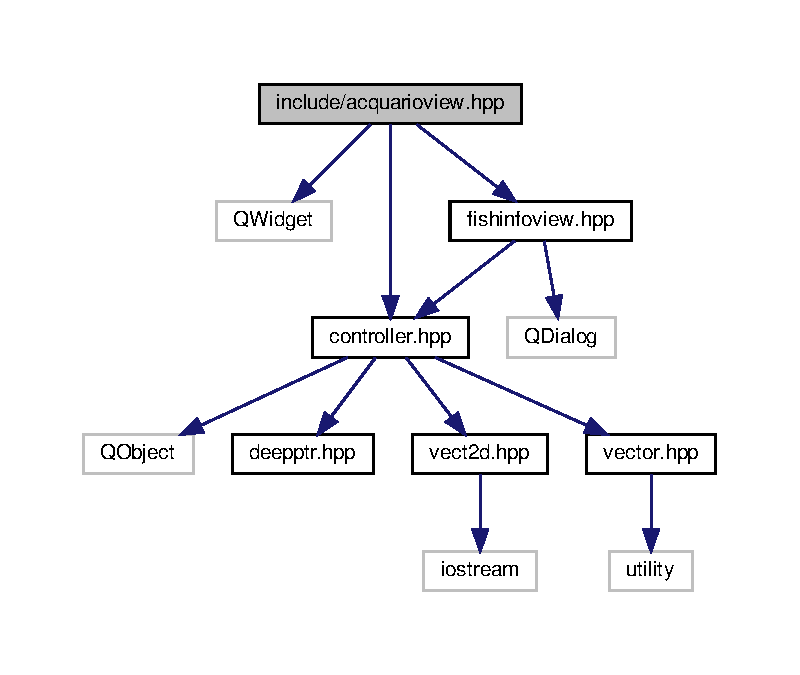
\includegraphics[width=350pt]{acquarioview_8hpp__incl}
\end{center}
\end{figure}
This graph shows which files directly or indirectly include this file\+:\nopagebreak
\begin{figure}[H]
\begin{center}
\leavevmode
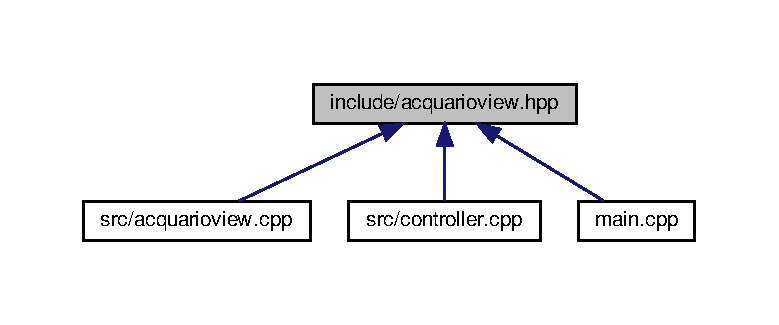
\includegraphics[width=350pt]{acquarioview_8hpp__dep__incl}
\end{center}
\end{figure}
\subsection*{Classes}
\begin{DoxyCompactItemize}
\item 
class \hyperlink{classAcquarioView}{Acquario\+View}
\end{DoxyCompactItemize}
\subsection*{Macros}
\begin{DoxyCompactItemize}
\item 
\#define \hyperlink{acquarioview_8hpp_aa72cbcc00b5bc16eade2d50ac3e48013_aa72cbcc00b5bc16eade2d50ac3e48013}{A\+C\+Q\+U\+A\+R\+I\+O\+V\+I\+E\+W\+\_\+H}
\end{DoxyCompactItemize}


\subsection{Macro Definition Documentation}
\mbox{\Hypertarget{acquarioview_8hpp_aa72cbcc00b5bc16eade2d50ac3e48013_aa72cbcc00b5bc16eade2d50ac3e48013}\label{acquarioview_8hpp_aa72cbcc00b5bc16eade2d50ac3e48013_aa72cbcc00b5bc16eade2d50ac3e48013}} 
\index{acquarioview.\+hpp@{acquarioview.\+hpp}!A\+C\+Q\+U\+A\+R\+I\+O\+V\+I\+E\+W\+\_\+H@{A\+C\+Q\+U\+A\+R\+I\+O\+V\+I\+E\+W\+\_\+H}}
\index{A\+C\+Q\+U\+A\+R\+I\+O\+V\+I\+E\+W\+\_\+H@{A\+C\+Q\+U\+A\+R\+I\+O\+V\+I\+E\+W\+\_\+H}!acquarioview.\+hpp@{acquarioview.\+hpp}}
\subsubsection{\texorpdfstring{A\+C\+Q\+U\+A\+R\+I\+O\+V\+I\+E\+W\+\_\+H}{ACQUARIOVIEW\_H}}
{\footnotesize\ttfamily \#define A\+C\+Q\+U\+A\+R\+I\+O\+V\+I\+E\+W\+\_\+H}


\hypertarget{aquarius_8hpp}{}\section{include/aquarius.hpp File Reference}
\label{aquarius_8hpp}\index{include/aquarius.\+hpp@{include/aquarius.\+hpp}}
{\ttfamily \#include \char`\"{}deepptr.\+hpp\char`\"{}}\newline
{\ttfamily \#include \char`\"{}fish.\+hpp\char`\"{}}\newline
{\ttfamily \#include \char`\"{}vector.\+hpp\char`\"{}}\newline
Include dependency graph for aquarius.\+hpp\+:\nopagebreak
\begin{figure}[H]
\begin{center}
\leavevmode
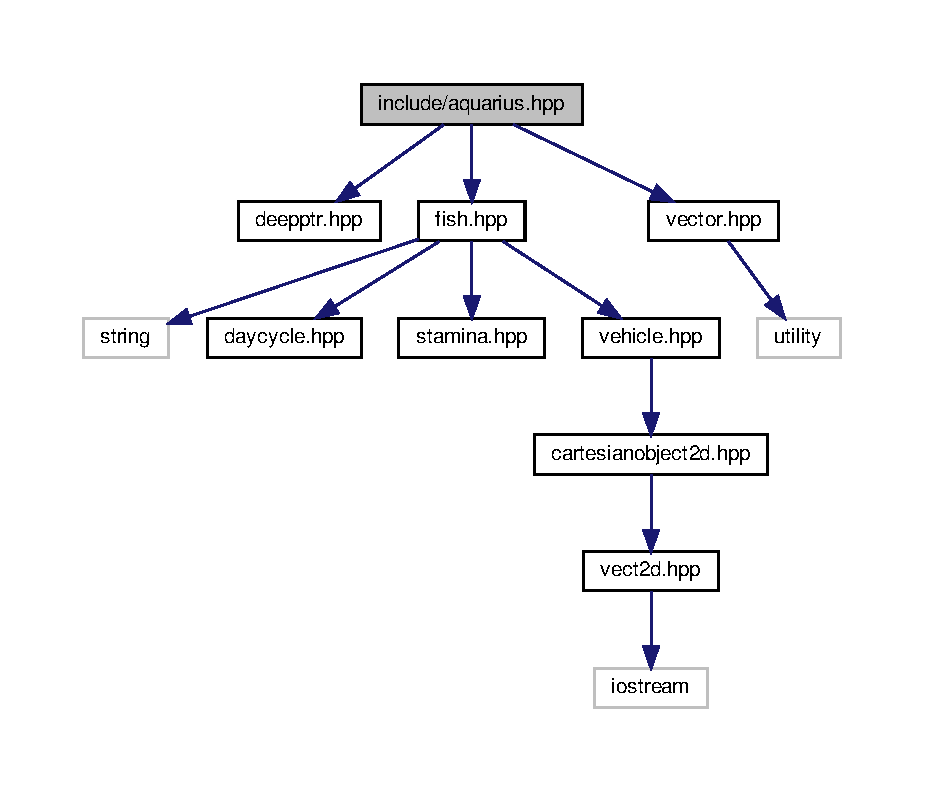
\includegraphics[width=350pt]{aquarius_8hpp__incl}
\end{center}
\end{figure}
This graph shows which files directly or indirectly include this file\+:\nopagebreak
\begin{figure}[H]
\begin{center}
\leavevmode
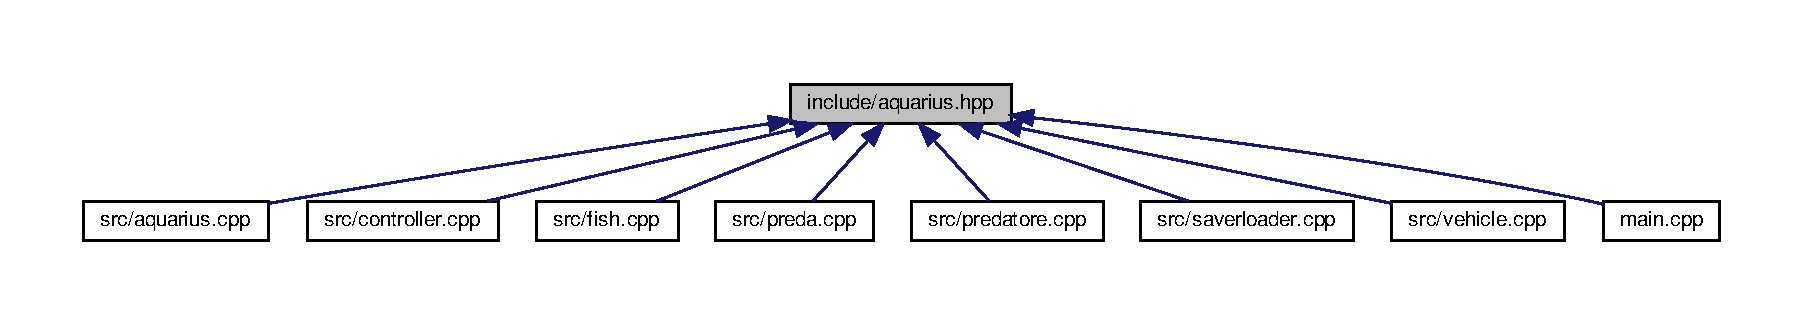
\includegraphics[width=350pt]{aquarius_8hpp__dep__incl}
\end{center}
\end{figure}
\subsection*{Classes}
\begin{DoxyCompactItemize}
\item 
class \hyperlink{classAquarius}{Aquarius}
\end{DoxyCompactItemize}
\subsection*{Macros}
\begin{DoxyCompactItemize}
\item 
\#define \hyperlink{aquarius_8hpp_a097667dfd52a1de88c739e2d800e426f_a097667dfd52a1de88c739e2d800e426f}{A\+Q\+U\+A\+R\+I\+U\+S\+\_\+H}
\end{DoxyCompactItemize}


\subsection{Macro Definition Documentation}
\mbox{\Hypertarget{aquarius_8hpp_a097667dfd52a1de88c739e2d800e426f_a097667dfd52a1de88c739e2d800e426f}\label{aquarius_8hpp_a097667dfd52a1de88c739e2d800e426f_a097667dfd52a1de88c739e2d800e426f}} 
\index{aquarius.\+hpp@{aquarius.\+hpp}!A\+Q\+U\+A\+R\+I\+U\+S\+\_\+H@{A\+Q\+U\+A\+R\+I\+U\+S\+\_\+H}}
\index{A\+Q\+U\+A\+R\+I\+U\+S\+\_\+H@{A\+Q\+U\+A\+R\+I\+U\+S\+\_\+H}!aquarius.\+hpp@{aquarius.\+hpp}}
\subsubsection{\texorpdfstring{A\+Q\+U\+A\+R\+I\+U\+S\+\_\+H}{AQUARIUS\_H}}
{\footnotesize\ttfamily \#define A\+Q\+U\+A\+R\+I\+U\+S\+\_\+H}


\hypertarget{bsptree_8hpp}{}\section{include/bsptree.hpp File Reference}
\label{bsptree_8hpp}\index{include/bsptree.\+hpp@{include/bsptree.\+hpp}}
{\ttfamily \#include $<$map$>$}\newline
{\ttfamily \#include $<$tuple$>$}\newline
{\ttfamily \#include $<$vector$>$}\newline
{\ttfamily \#include \char`\"{}vect2d.\+hpp\char`\"{}}\newline
Include dependency graph for bsptree.\+hpp\+:\nopagebreak
\begin{figure}[H]
\begin{center}
\leavevmode
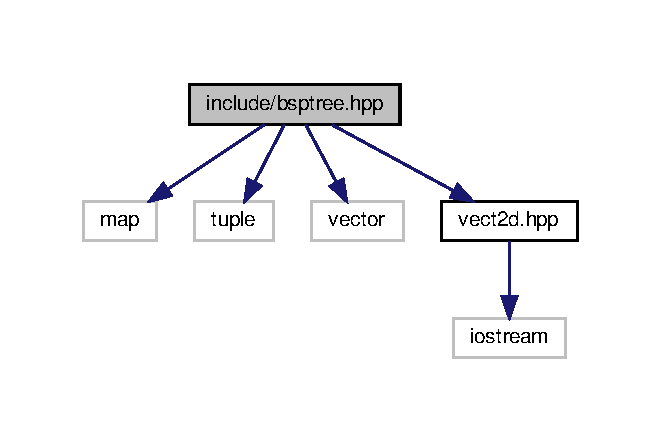
\includegraphics[width=317pt]{bsptree_8hpp__incl}
\end{center}
\end{figure}
\subsection*{Classes}
\begin{DoxyCompactItemize}
\item 
class \hyperlink{classRange}{Range}
\item 
class \hyperlink{classBSPTree}{B\+S\+P\+Tree$<$ T $>$}
\end{DoxyCompactItemize}

\hypertarget{cartesianobject2d_8hpp}{}\section{include/cartesianobject2d.hpp File Reference}
\label{cartesianobject2d_8hpp}\index{include/cartesianobject2d.\+hpp@{include/cartesianobject2d.\+hpp}}
{\ttfamily \#include \char`\"{}vect2d.\+hpp\char`\"{}}\newline
Include dependency graph for cartesianobject2d.\+hpp\+:\nopagebreak
\begin{figure}[H]
\begin{center}
\leavevmode
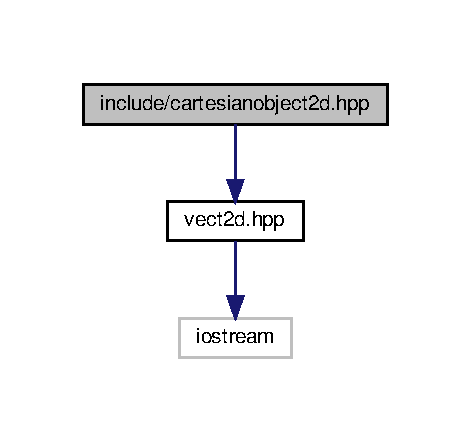
\includegraphics[width=226pt]{cartesianobject2d_8hpp__incl}
\end{center}
\end{figure}
This graph shows which files directly or indirectly include this file\+:\nopagebreak
\begin{figure}[H]
\begin{center}
\leavevmode
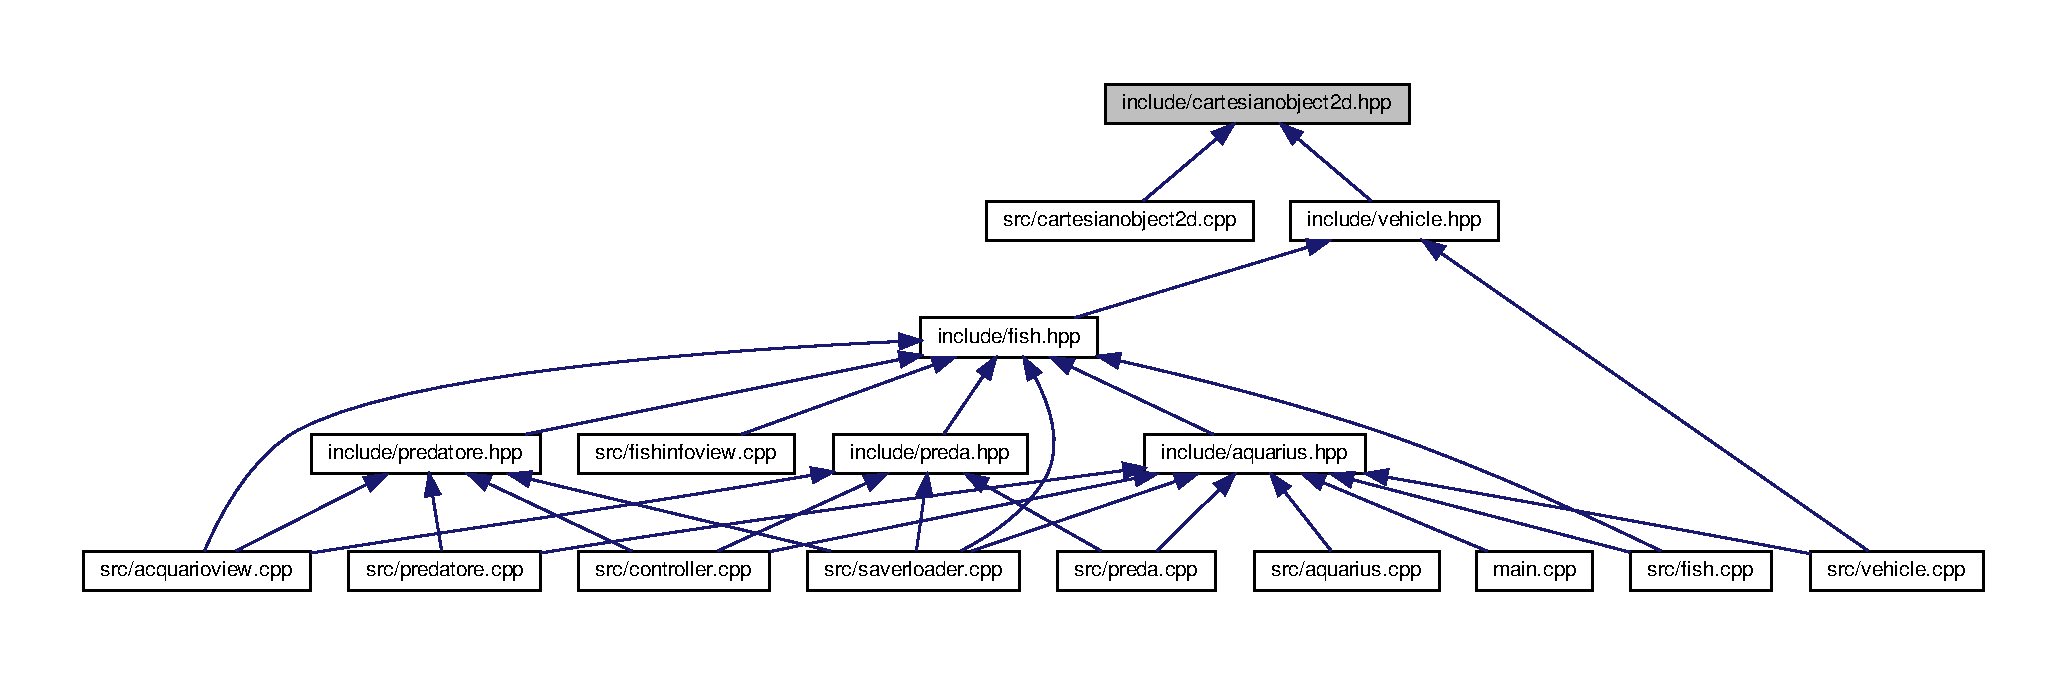
\includegraphics[width=350pt]{cartesianobject2d_8hpp__dep__incl}
\end{center}
\end{figure}
\subsection*{Classes}
\begin{DoxyCompactItemize}
\item 
class \hyperlink{classCartesianObject2D}{Cartesian\+Object2D}
\end{DoxyCompactItemize}

\hypertarget{controller_8hpp}{}\section{include/controller.hpp File Reference}
\label{controller_8hpp}\index{include/controller.\+hpp@{include/controller.\+hpp}}
{\ttfamily \#include $<$Q\+Object$>$}\newline
{\ttfamily \#include \char`\"{}deepptr.\+hpp\char`\"{}}\newline
{\ttfamily \#include \char`\"{}vect2d.\+hpp\char`\"{}}\newline
{\ttfamily \#include \char`\"{}vector.\+hpp\char`\"{}}\newline
Include dependency graph for controller.\+hpp\+:\nopagebreak
\begin{figure}[H]
\begin{center}
\leavevmode
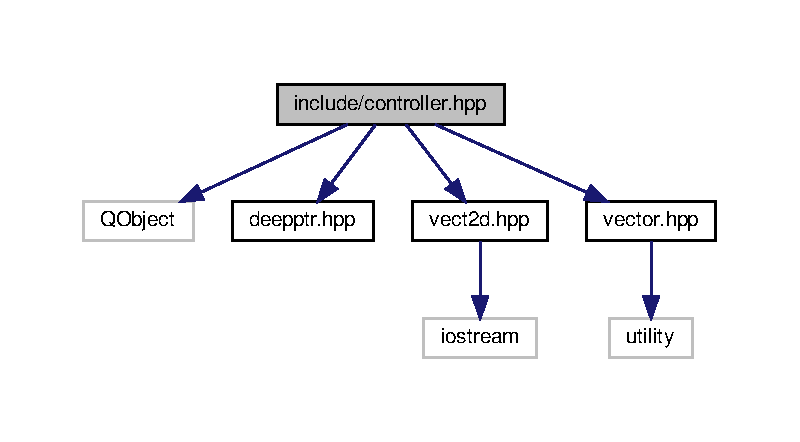
\includegraphics[width=350pt]{controller_8hpp__incl}
\end{center}
\end{figure}
This graph shows which files directly or indirectly include this file\+:\nopagebreak
\begin{figure}[H]
\begin{center}
\leavevmode
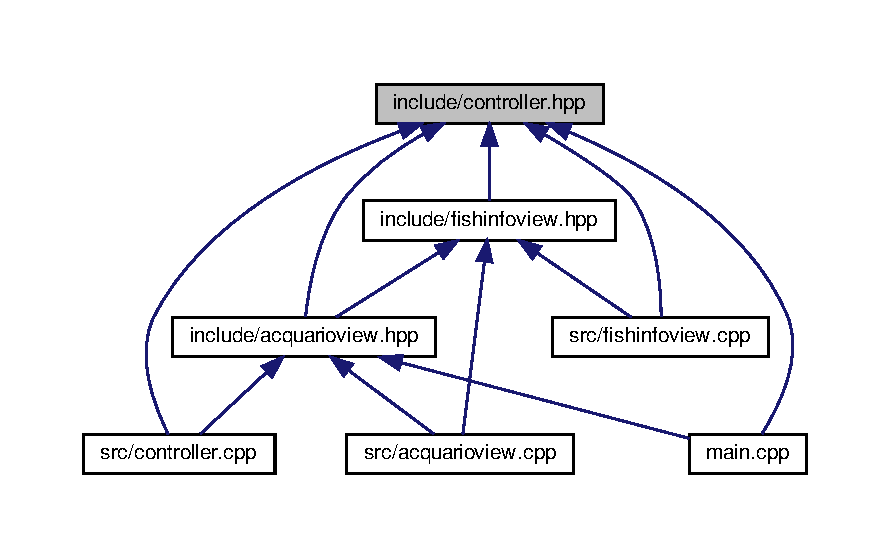
\includegraphics[width=350pt]{controller_8hpp__dep__incl}
\end{center}
\end{figure}
\subsection*{Classes}
\begin{DoxyCompactItemize}
\item 
class \hyperlink{classController}{Controller}
\end{DoxyCompactItemize}

\hypertarget{daycycle_8hpp}{}\section{include/daycycle.hpp File Reference}
\label{daycycle_8hpp}\index{include/daycycle.\+hpp@{include/daycycle.\+hpp}}
This graph shows which files directly or indirectly include this file\+:\nopagebreak
\begin{figure}[H]
\begin{center}
\leavevmode
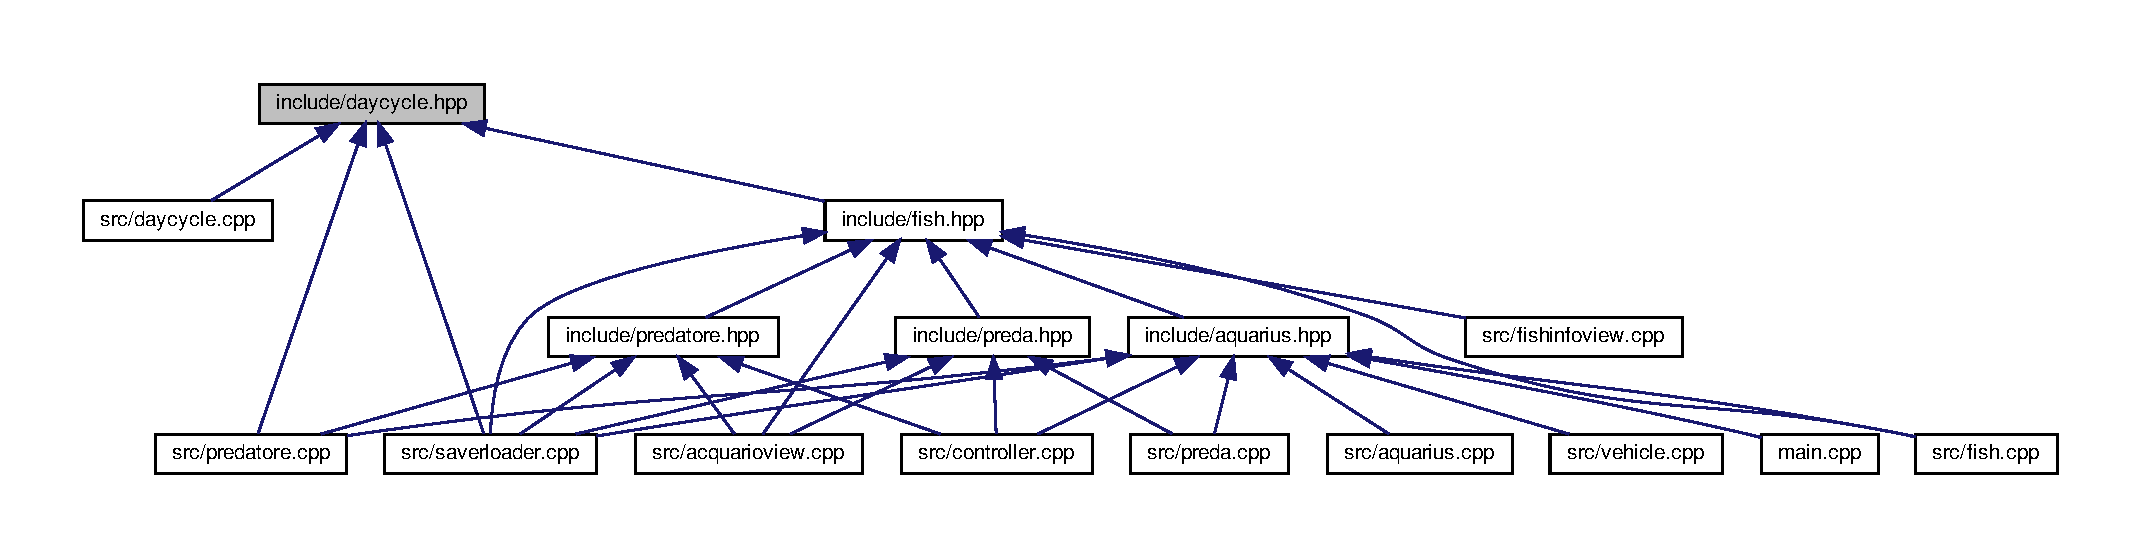
\includegraphics[width=350pt]{daycycle_8hpp__dep__incl}
\end{center}
\end{figure}
\subsection*{Classes}
\begin{DoxyCompactItemize}
\item 
class \hyperlink{classDayCycle}{Day\+Cycle}
\end{DoxyCompactItemize}

\hypertarget{deepptr_8hpp}{}\section{include/deepptr.hpp File Reference}
\label{deepptr_8hpp}\index{include/deepptr.\+hpp@{include/deepptr.\+hpp}}
This graph shows which files directly or indirectly include this file\+:\nopagebreak
\begin{figure}[H]
\begin{center}
\leavevmode
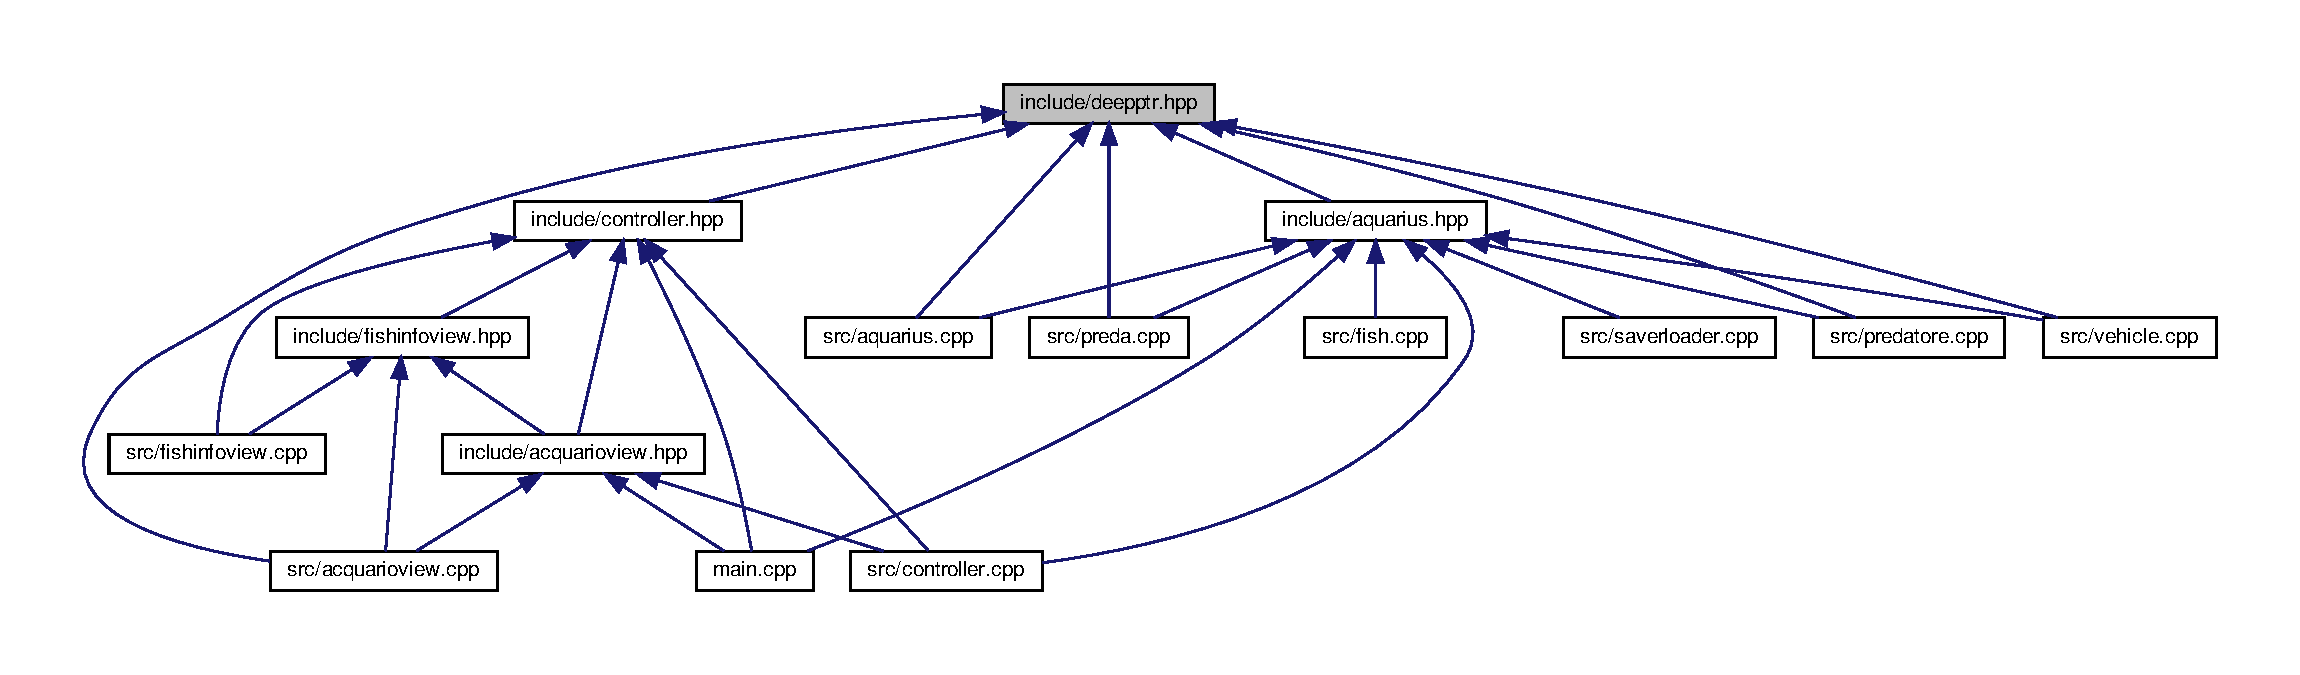
\includegraphics[width=350pt]{deepptr_8hpp__dep__incl}
\end{center}
\end{figure}
\subsection*{Classes}
\begin{DoxyCompactItemize}
\item 
class \hyperlink{classDeepPtr}{Deep\+Ptr$<$ T $>$}
\end{DoxyCompactItemize}

\hypertarget{fish_8hpp}{}\section{include/fish.hpp File Reference}
\label{fish_8hpp}\index{include/fish.\+hpp@{include/fish.\+hpp}}
{\ttfamily \#include $<$string$>$}\newline
{\ttfamily \#include \char`\"{}daycycle.\+hpp\char`\"{}}\newline
{\ttfamily \#include \char`\"{}stamina.\+hpp\char`\"{}}\newline
{\ttfamily \#include \char`\"{}vehicle.\+hpp\char`\"{}}\newline
Include dependency graph for fish.\+hpp\+:\nopagebreak
\begin{figure}[H]
\begin{center}
\leavevmode
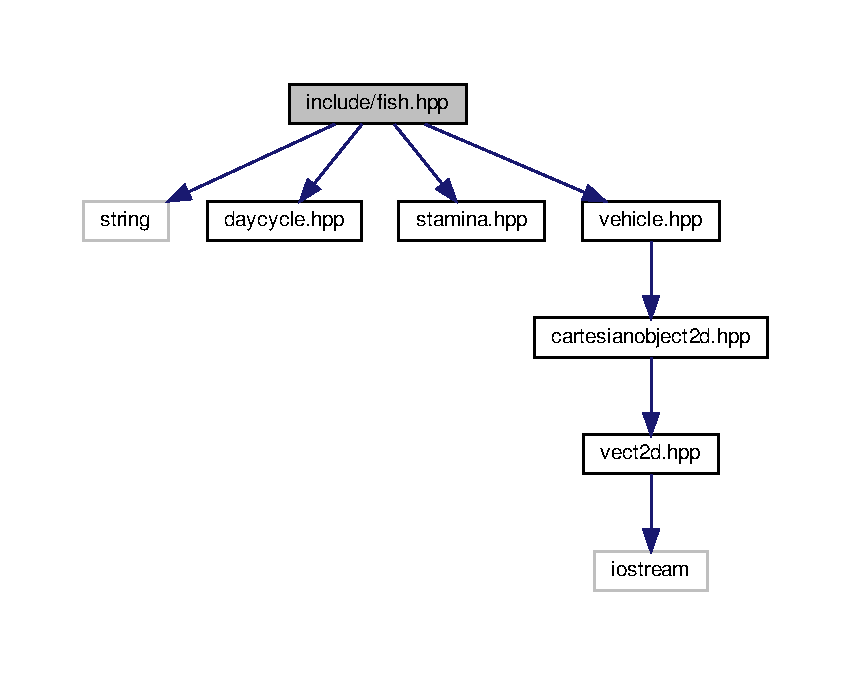
\includegraphics[width=350pt]{fish_8hpp__incl}
\end{center}
\end{figure}
This graph shows which files directly or indirectly include this file\+:\nopagebreak
\begin{figure}[H]
\begin{center}
\leavevmode
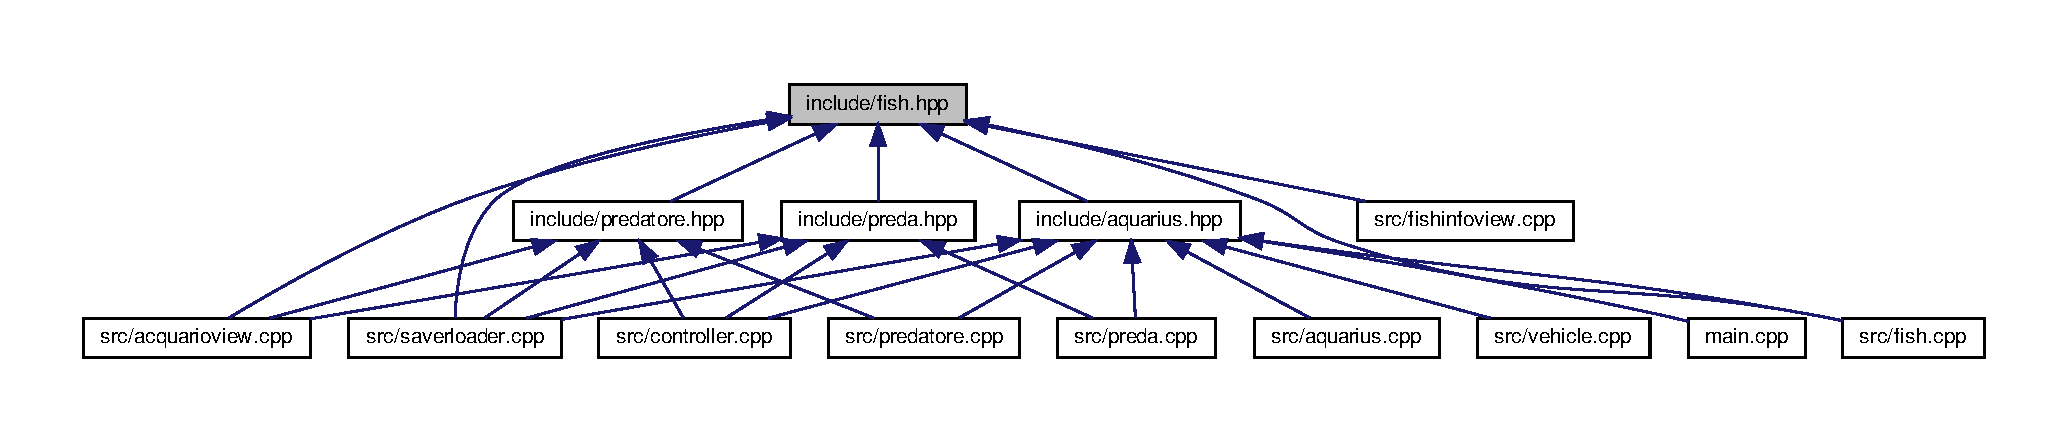
\includegraphics[width=350pt]{fish_8hpp__dep__incl}
\end{center}
\end{figure}
\subsection*{Classes}
\begin{DoxyCompactItemize}
\item 
class \hyperlink{classFish}{Fish}
\end{DoxyCompactItemize}

\hypertarget{fishinfoview_8hpp}{}\section{include/fishinfoview.hpp File Reference}
\label{fishinfoview_8hpp}\index{include/fishinfoview.\+hpp@{include/fishinfoview.\+hpp}}
{\ttfamily \#include $<$Q\+Dialog$>$}\newline
{\ttfamily \#include \char`\"{}controller.\+hpp\char`\"{}}\newline
Include dependency graph for fishinfoview.\+hpp\+:\nopagebreak
\begin{figure}[H]
\begin{center}
\leavevmode
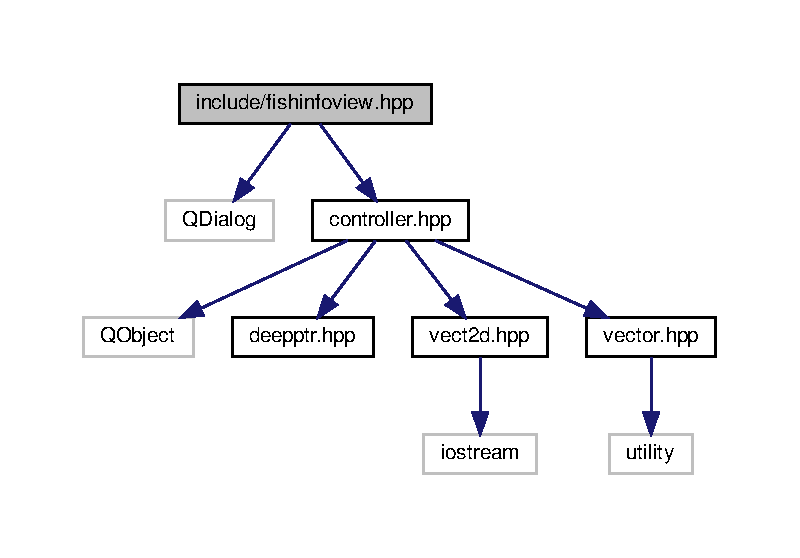
\includegraphics[width=350pt]{fishinfoview_8hpp__incl}
\end{center}
\end{figure}
This graph shows which files directly or indirectly include this file\+:\nopagebreak
\begin{figure}[H]
\begin{center}
\leavevmode
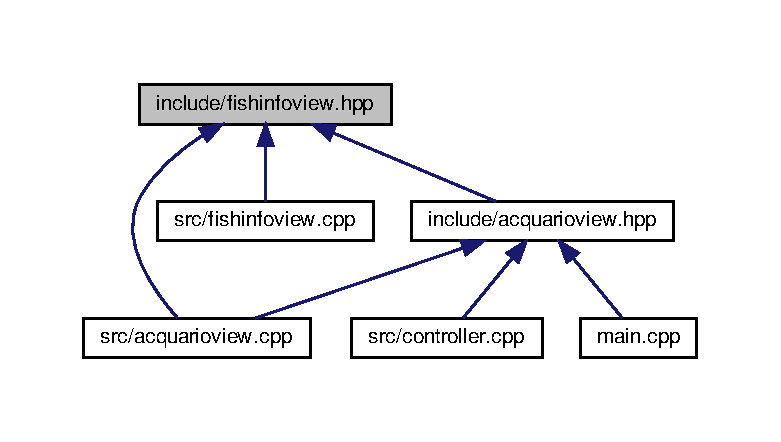
\includegraphics[width=350pt]{fishinfoview_8hpp__dep__incl}
\end{center}
\end{figure}
\subsection*{Classes}
\begin{DoxyCompactItemize}
\item 
class \hyperlink{classFishInfoView}{Fish\+Info\+View}
\end{DoxyCompactItemize}

\hypertarget{preda_8hpp}{}\section{include/preda.hpp File Reference}
\label{preda_8hpp}\index{include/preda.\+hpp@{include/preda.\+hpp}}
{\ttfamily \#include \char`\"{}fish.\+hpp\char`\"{}}\newline
Include dependency graph for preda.\+hpp\+:\nopagebreak
\begin{figure}[H]
\begin{center}
\leavevmode
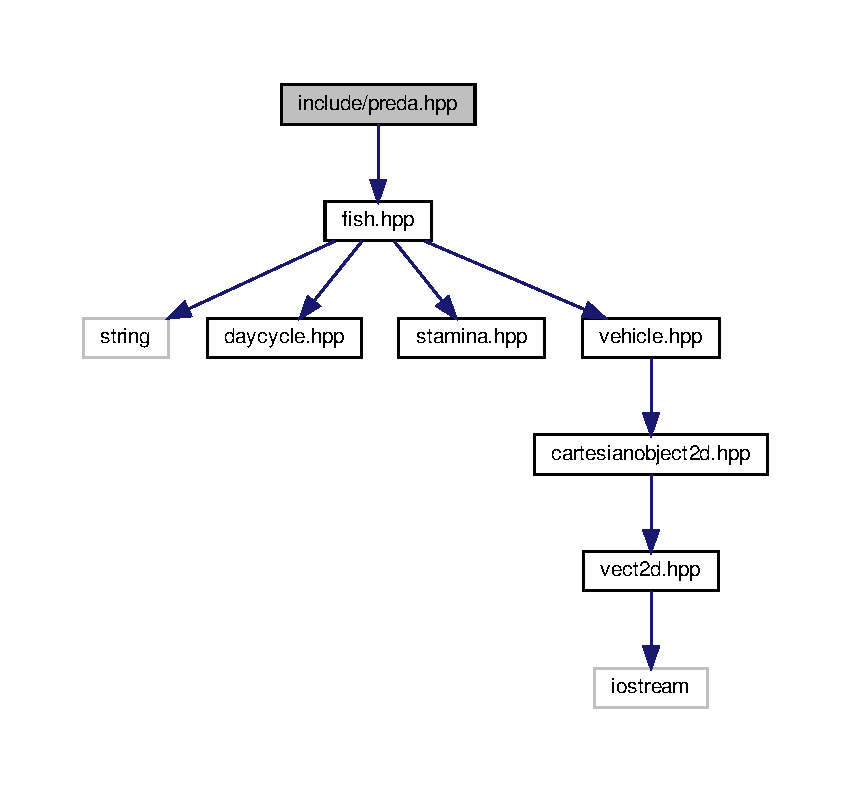
\includegraphics[width=350pt]{preda_8hpp__incl}
\end{center}
\end{figure}
This graph shows which files directly or indirectly include this file\+:\nopagebreak
\begin{figure}[H]
\begin{center}
\leavevmode
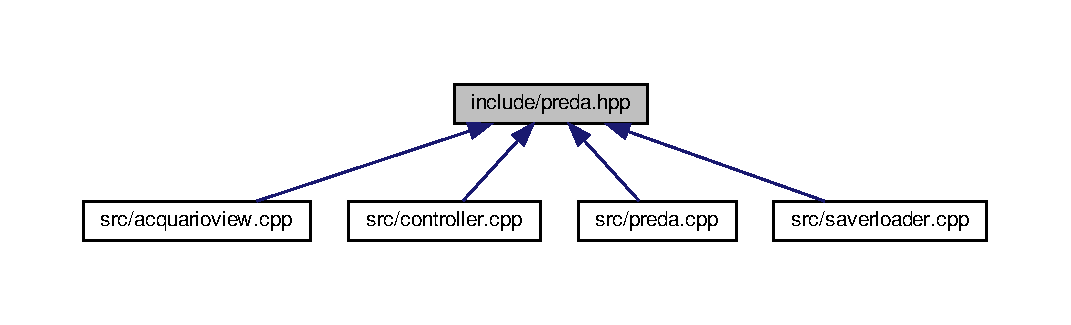
\includegraphics[width=350pt]{preda_8hpp__dep__incl}
\end{center}
\end{figure}
\subsection*{Classes}
\begin{DoxyCompactItemize}
\item 
class \hyperlink{classPreda}{Preda}
\end{DoxyCompactItemize}

\hypertarget{predatore_8hpp}{}\section{include/predatore.hpp File Reference}
\label{predatore_8hpp}\index{include/predatore.\+hpp@{include/predatore.\+hpp}}
{\ttfamily \#include \char`\"{}fish.\+hpp\char`\"{}}\newline
Include dependency graph for predatore.\+hpp\+:\nopagebreak
\begin{figure}[H]
\begin{center}
\leavevmode
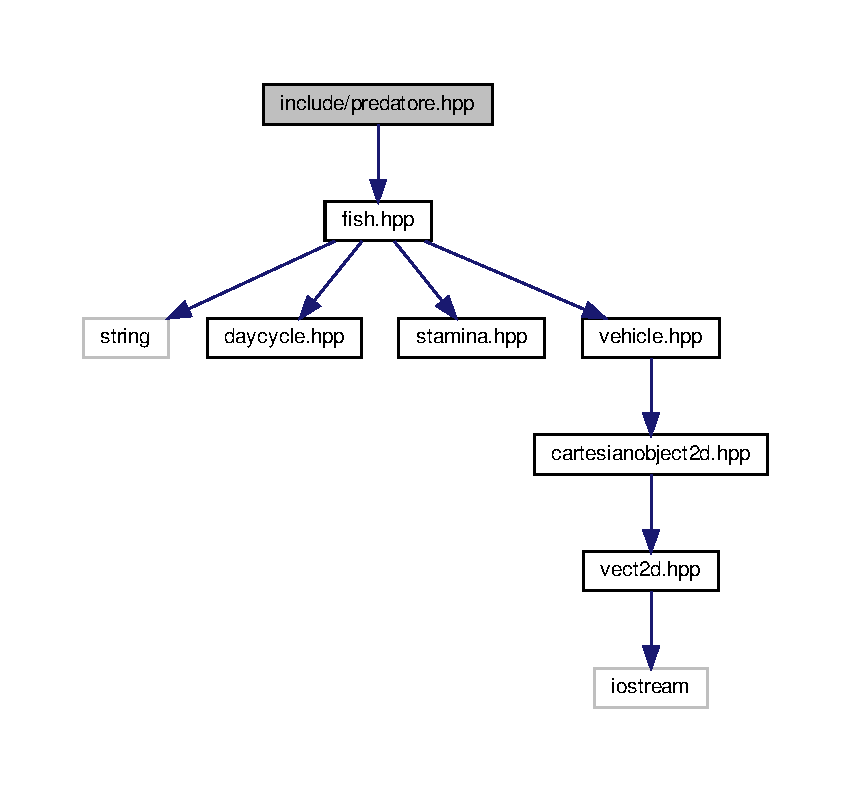
\includegraphics[width=350pt]{predatore_8hpp__incl}
\end{center}
\end{figure}
This graph shows which files directly or indirectly include this file\+:\nopagebreak
\begin{figure}[H]
\begin{center}
\leavevmode
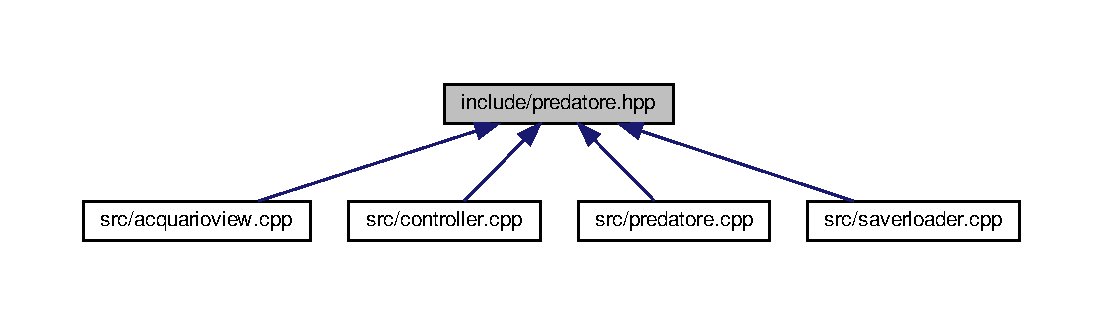
\includegraphics[width=350pt]{predatore_8hpp__dep__incl}
\end{center}
\end{figure}
\subsection*{Classes}
\begin{DoxyCompactItemize}
\item 
class \hyperlink{classPredatore}{Predatore}
\end{DoxyCompactItemize}

\hypertarget{stamina_8hpp}{}\section{include/stamina.hpp File Reference}
\label{stamina_8hpp}\index{include/stamina.\+hpp@{include/stamina.\+hpp}}
This graph shows which files directly or indirectly include this file\+:\nopagebreak
\begin{figure}[H]
\begin{center}
\leavevmode
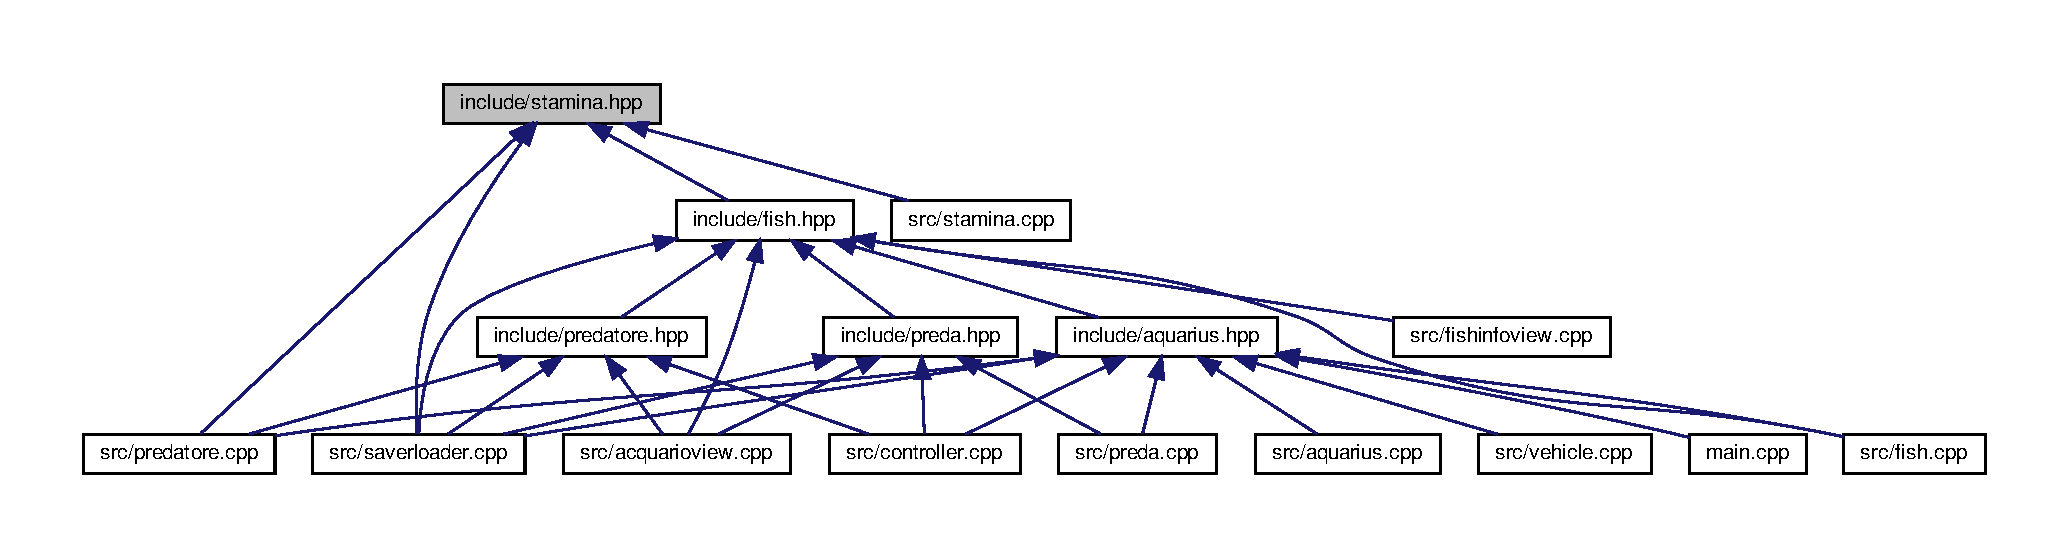
\includegraphics[width=350pt]{stamina_8hpp__dep__incl}
\end{center}
\end{figure}
\subsection*{Classes}
\begin{DoxyCompactItemize}
\item 
class \hyperlink{classStamina}{Stamina}
\end{DoxyCompactItemize}

\hypertarget{vect2d_8hpp}{}\section{include/vect2d.hpp File Reference}
\label{vect2d_8hpp}\index{include/vect2d.\+hpp@{include/vect2d.\+hpp}}
{\ttfamily \#include $<$iostream$>$}\newline
Include dependency graph for vect2d.\+hpp\+:\nopagebreak
\begin{figure}[H]
\begin{center}
\leavevmode
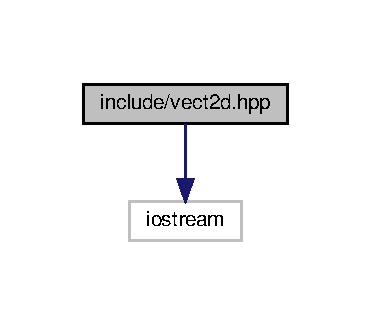
\includegraphics[width=178pt]{vect2d_8hpp__incl}
\end{center}
\end{figure}
This graph shows which files directly or indirectly include this file\+:\nopagebreak
\begin{figure}[H]
\begin{center}
\leavevmode
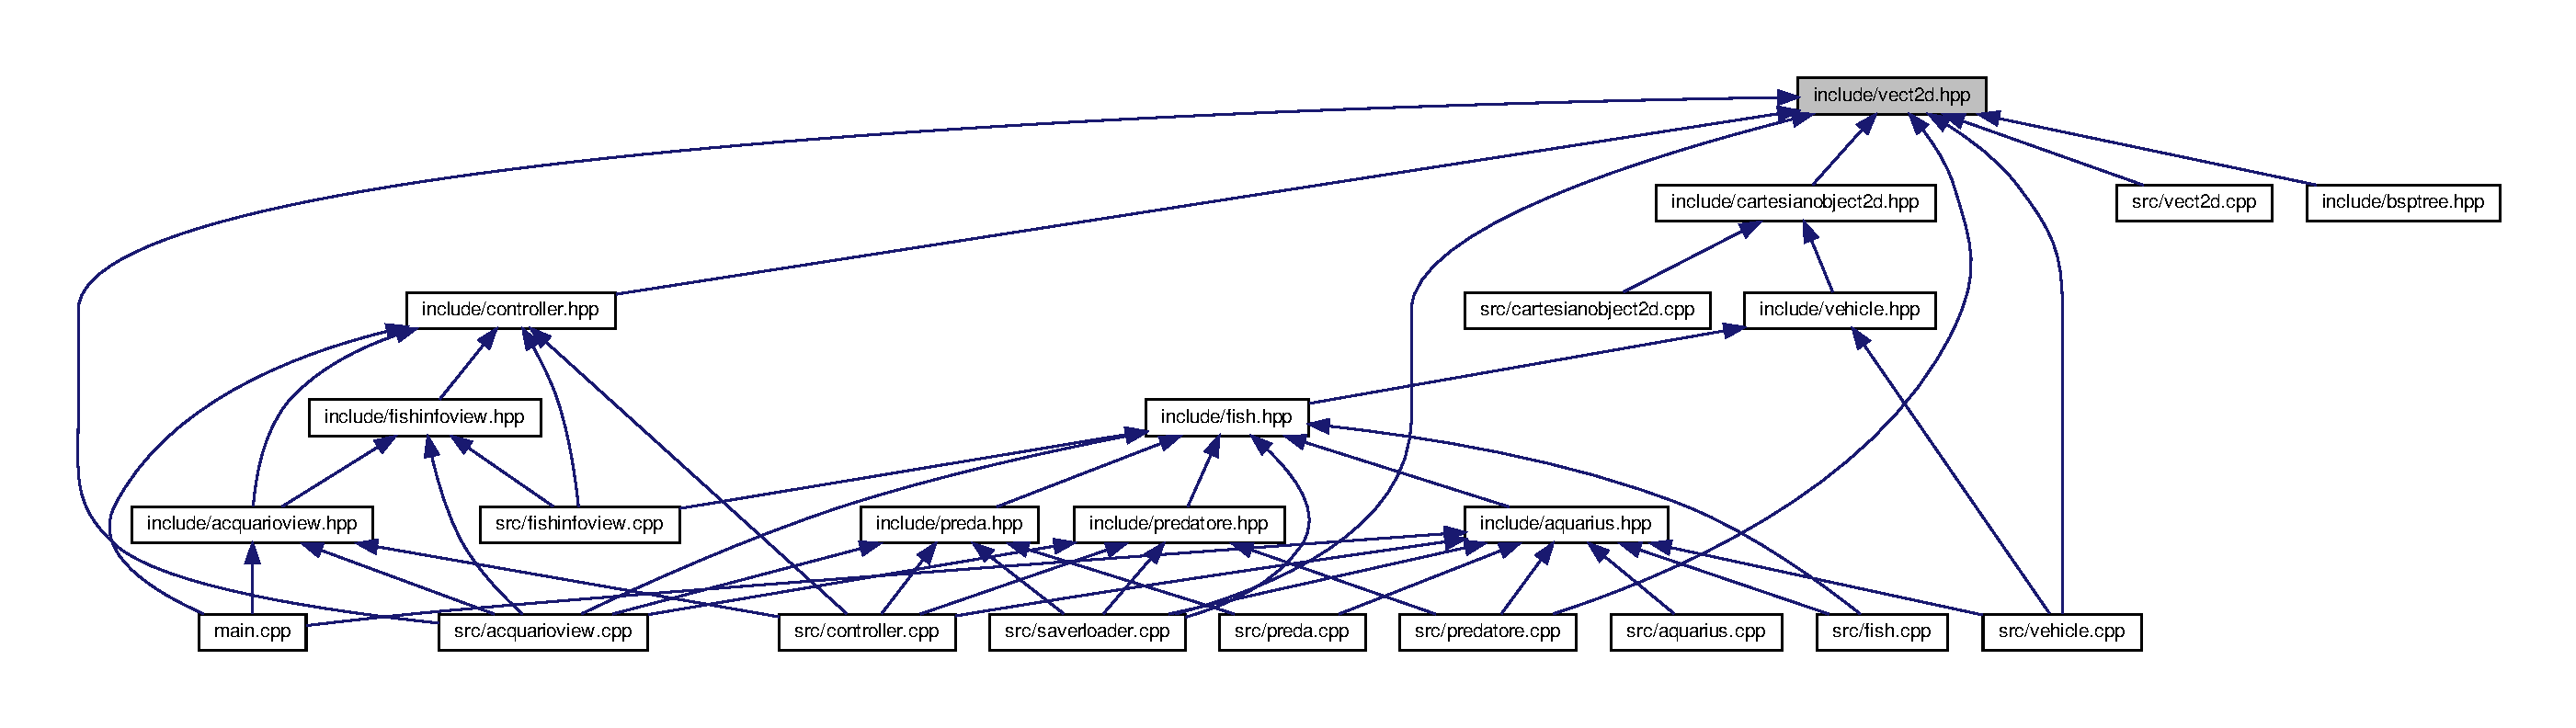
\includegraphics[width=350pt]{vect2d_8hpp__dep__incl}
\end{center}
\end{figure}
\subsection*{Classes}
\begin{DoxyCompactItemize}
\item 
class \hyperlink{classVect2D}{Vect2D}
\end{DoxyCompactItemize}

\hypertarget{vector_8hpp}{}\section{include/vector.hpp File Reference}
\label{vector_8hpp}\index{include/vector.\+hpp@{include/vector.\+hpp}}
{\ttfamily \#include $<$utility$>$}\newline
Include dependency graph for vector.\+hpp\+:\nopagebreak
\begin{figure}[H]
\begin{center}
\leavevmode
\includegraphics[width=176pt]{vector_8hpp__incl}
\end{center}
\end{figure}
This graph shows which files directly or indirectly include this file\+:\nopagebreak
\begin{figure}[H]
\begin{center}
\leavevmode
\includegraphics[width=350pt]{vector_8hpp__dep__incl}
\end{center}
\end{figure}
\subsection*{Classes}
\begin{DoxyCompactItemize}
\item 
class \hyperlink{classVector}{Vector$<$ T $>$}
\item 
class \hyperlink{classVector_1_1iterator}{Vector$<$ T $>$\+::iterator}
\item 
class \hyperlink{classVector_1_1const__iterator}{Vector$<$ T $>$\+::const\+\_\+iterator}
\end{DoxyCompactItemize}

\hypertarget{vehicle_8hpp}{}\section{include/vehicle.hpp File Reference}
\label{vehicle_8hpp}\index{include/vehicle.\+hpp@{include/vehicle.\+hpp}}
{\ttfamily \#include \char`\"{}cartesianobject2d.\+hpp\char`\"{}}\newline
Include dependency graph for vehicle.\+hpp\+:\nopagebreak
\begin{figure}[H]
\begin{center}
\leavevmode
\includegraphics[width=192pt]{vehicle_8hpp__incl}
\end{center}
\end{figure}
This graph shows which files directly or indirectly include this file\+:\nopagebreak
\begin{figure}[H]
\begin{center}
\leavevmode
\includegraphics[width=350pt]{vehicle_8hpp__dep__incl}
\end{center}
\end{figure}
\subsection*{Classes}
\begin{DoxyCompactItemize}
\item 
class \hyperlink{classVehicle}{Vehicle}
\end{DoxyCompactItemize}

\hypertarget{main_8cpp}{}\section{main.\+cpp File Reference}
\label{main_8cpp}\index{main.\+cpp@{main.\+cpp}}
{\ttfamily \#include $<$Q\+Application$>$}\newline
{\ttfamily \#include \char`\"{}acquarioview.\+hpp\char`\"{}}\newline
{\ttfamily \#include \char`\"{}aquarius.\+hpp\char`\"{}}\newline
{\ttfamily \#include \char`\"{}controller.\+hpp\char`\"{}}\newline
Include dependency graph for main.\+cpp\+:\nopagebreak
\begin{figure}[H]
\begin{center}
\leavevmode
\includegraphics[width=350pt]{main_8cpp__incl}
\end{center}
\end{figure}
\subsection*{Functions}
\begin{DoxyCompactItemize}
\item 
int \hyperlink{main_8cpp_a0ddf1224851353fc92bfbff6f499fa97_a0ddf1224851353fc92bfbff6f499fa97}{main} (int argc, char $\ast$argv\mbox{[}$\,$\mbox{]})
\end{DoxyCompactItemize}


\subsection{Function Documentation}
\mbox{\Hypertarget{main_8cpp_a0ddf1224851353fc92bfbff6f499fa97_a0ddf1224851353fc92bfbff6f499fa97}\label{main_8cpp_a0ddf1224851353fc92bfbff6f499fa97_a0ddf1224851353fc92bfbff6f499fa97}} 
\index{main.\+cpp@{main.\+cpp}!main@{main}}
\index{main@{main}!main.\+cpp@{main.\+cpp}}
\subsubsection{\texorpdfstring{main()}{main()}}
{\footnotesize\ttfamily int main (\begin{DoxyParamCaption}\item[{int}]{argc,  }\item[{char $\ast$}]{argv\mbox{[}$\,$\mbox{]} }\end{DoxyParamCaption})}


\hypertarget{acquarioview_8cpp}{}\section{src/acquarioview.cpp File Reference}
\label{acquarioview_8cpp}\index{src/acquarioview.\+cpp@{src/acquarioview.\+cpp}}
{\ttfamily \#include \char`\"{}acquarioview.\+hpp\char`\"{}}\newline
{\ttfamily \#include $<$Q\+Menu\+Bar$>$}\newline
{\ttfamily \#include $<$Q\+Paint\+Event$>$}\newline
{\ttfamily \#include $<$Q\+Painter$>$}\newline
{\ttfamily \#include $<$Q\+V\+Box\+Layout$>$}\newline
{\ttfamily \#include \char`\"{}deepptr.\+hpp\char`\"{}}\newline
{\ttfamily \#include \char`\"{}fish.\+hpp\char`\"{}}\newline
{\ttfamily \#include \char`\"{}fishinfoview.\+hpp\char`\"{}}\newline
{\ttfamily \#include \char`\"{}preda.\+hpp\char`\"{}}\newline
{\ttfamily \#include \char`\"{}predatore.\+hpp\char`\"{}}\newline
{\ttfamily \#include \char`\"{}vect2d.\+hpp\char`\"{}}\newline
Include dependency graph for acquarioview.\+cpp\+:\nopagebreak
\begin{figure}[H]
\begin{center}
\leavevmode
\includegraphics[width=350pt]{acquarioview_8cpp__incl}
\end{center}
\end{figure}

\hypertarget{aquarius_8cpp}{}\section{src/aquarius.cpp File Reference}
\label{aquarius_8cpp}\index{src/aquarius.\+cpp@{src/aquarius.\+cpp}}
{\ttfamily \#include \char`\"{}aquarius.\+hpp\char`\"{}}\newline
{\ttfamily \#include \char`\"{}deepptr.\+hpp\char`\"{}}\newline
{\ttfamily \#include \char`\"{}vector.\+hpp\char`\"{}}\newline
Include dependency graph for aquarius.\+cpp\+:\nopagebreak
\begin{figure}[H]
\begin{center}
\leavevmode
\includegraphics[width=350pt]{aquarius_8cpp__incl}
\end{center}
\end{figure}

\hypertarget{cartesianobject2d_8cpp}{}\section{src/cartesianobject2d.cpp File Reference}
\label{cartesianobject2d_8cpp}\index{src/cartesianobject2d.\+cpp@{src/cartesianobject2d.\+cpp}}
{\ttfamily \#include \char`\"{}cartesianobject2d.\+hpp\char`\"{}}\newline
Include dependency graph for cartesianobject2d.\+cpp\+:\nopagebreak
\begin{figure}[H]
\begin{center}
\leavevmode
\includegraphics[width=208pt]{cartesianobject2d_8cpp__incl}
\end{center}
\end{figure}

\hypertarget{controller_8cpp}{}\section{src/controller.cpp File Reference}
\label{controller_8cpp}\index{src/controller.\+cpp@{src/controller.\+cpp}}
{\ttfamily \#include \char`\"{}controller.\+hpp\char`\"{}}\newline
{\ttfamily \#include $<$Q\+Object$>$}\newline
{\ttfamily \#include $<$Q\+Timer$>$}\newline
{\ttfamily \#include \char`\"{}acquarioview.\+hpp\char`\"{}}\newline
{\ttfamily \#include \char`\"{}aquarius.\+hpp\char`\"{}}\newline
{\ttfamily \#include \char`\"{}preda.\+hpp\char`\"{}}\newline
{\ttfamily \#include \char`\"{}predatore.\+hpp\char`\"{}}\newline
Include dependency graph for controller.\+cpp\+:\nopagebreak
\begin{figure}[H]
\begin{center}
\leavevmode
\includegraphics[width=350pt]{controller_8cpp__incl}
\end{center}
\end{figure}

\hypertarget{daycycle_8cpp}{}\section{src/daycycle.cpp File Reference}
\label{daycycle_8cpp}\index{src/daycycle.\+cpp@{src/daycycle.\+cpp}}
{\ttfamily \#include \char`\"{}daycycle.\+hpp\char`\"{}}\newline
Include dependency graph for daycycle.\+cpp\+:\nopagebreak
\begin{figure}[H]
\begin{center}
\leavevmode
\includegraphics[width=171pt]{daycycle_8cpp__incl}
\end{center}
\end{figure}

\hypertarget{fish_8cpp}{}\section{src/fish.cpp File Reference}
\label{fish_8cpp}\index{src/fish.\+cpp@{src/fish.\+cpp}}
{\ttfamily \#include \char`\"{}fish.\+hpp\char`\"{}}\newline
{\ttfamily \#include \char`\"{}aquarius.\+hpp\char`\"{}}\newline
Include dependency graph for fish.\+cpp\+:\nopagebreak
\begin{figure}[H]
\begin{center}
\leavevmode
\includegraphics[width=350pt]{fish_8cpp__incl}
\end{center}
\end{figure}

\hypertarget{fishinfoview_8cpp}{}\section{src/fishinfoview.cpp File Reference}
\label{fishinfoview_8cpp}\index{src/fishinfoview.\+cpp@{src/fishinfoview.\+cpp}}
{\ttfamily \#include \char`\"{}fishinfoview.\+hpp\char`\"{}}\newline
{\ttfamily \#include \char`\"{}fish.\+hpp\char`\"{}}\newline
{\ttfamily \#include $<$Q\+Grid\+Layout$>$}\newline
{\ttfamily \#include $<$Q\+Label$>$}\newline
{\ttfamily \#include $<$Q\+Line\+Edit$>$}\newline
{\ttfamily \#include $<$Q\+Progress\+Bar$>$}\newline
{\ttfamily \#include $<$Q\+Push\+Button$>$}\newline
{\ttfamily \#include $<$controller.\+hpp$>$}\newline
{\ttfamily \#include $<$sstream$>$}\newline
Include dependency graph for fishinfoview.\+cpp\+:\nopagebreak
\begin{figure}[H]
\begin{center}
\leavevmode
\includegraphics[width=350pt]{fishinfoview_8cpp__incl}
\end{center}
\end{figure}

\hypertarget{fishview_8cpp}{}\section{src/fishview.cpp File Reference}
\label{fishview_8cpp}\index{src/fishview.\+cpp@{src/fishview.\+cpp}}

\hypertarget{preda_8cpp}{}\section{src/preda.cpp File Reference}
\label{preda_8cpp}\index{src/preda.\+cpp@{src/preda.\+cpp}}
{\ttfamily \#include \char`\"{}preda.\+hpp\char`\"{}}\newline
{\ttfamily \#include \char`\"{}aquarius.\+hpp\char`\"{}}\newline
{\ttfamily \#include \char`\"{}deepptr.\+hpp\char`\"{}}\newline
{\ttfamily \#include \char`\"{}vector.\+hpp\char`\"{}}\newline
Include dependency graph for preda.\+cpp\+:\nopagebreak
\begin{figure}[H]
\begin{center}
\leavevmode
\includegraphics[width=350pt]{preda_8cpp__incl}
\end{center}
\end{figure}

\hypertarget{predatore_8cpp}{}\section{src/predatore.cpp File Reference}
\label{predatore_8cpp}\index{src/predatore.\+cpp@{src/predatore.\+cpp}}
{\ttfamily \#include \char`\"{}predatore.\+hpp\char`\"{}}\newline
{\ttfamily \#include $<$iostream$>$}\newline
{\ttfamily \#include \char`\"{}aquarius.\+hpp\char`\"{}}\newline
{\ttfamily \#include \char`\"{}daycycle.\+hpp\char`\"{}}\newline
{\ttfamily \#include \char`\"{}deepptr.\+hpp\char`\"{}}\newline
{\ttfamily \#include \char`\"{}stamina.\+hpp\char`\"{}}\newline
{\ttfamily \#include \char`\"{}vect2d.\+hpp\char`\"{}}\newline
Include dependency graph for predatore.\+cpp\+:\nopagebreak
\begin{figure}[H]
\begin{center}
\leavevmode
\includegraphics[width=350pt]{predatore_8cpp__incl}
\end{center}
\end{figure}

\hypertarget{saverloader_8cpp}{}\section{src/saverloader.cpp File Reference}
\label{saverloader_8cpp}\index{src/saverloader.\+cpp@{src/saverloader.\+cpp}}
{\ttfamily \#include \char`\"{}middlewares/saverloader.\+hpp\char`\"{}}\newline
{\ttfamily \#include $<$Q\+File$>$}\newline
{\ttfamily \#include $<$Q\+Json\+Array$>$}\newline
{\ttfamily \#include $<$Q\+Json\+Document$>$}\newline
{\ttfamily \#include $<$Q\+Json\+Object$>$}\newline
{\ttfamily \#include $<$Q\+String$>$}\newline
{\ttfamily \#include $<$iostream$>$}\newline
{\ttfamily \#include $<$string$>$}\newline
{\ttfamily \#include \char`\"{}aquarius.\+hpp\char`\"{}}\newline
{\ttfamily \#include \char`\"{}daycycle.\+hpp\char`\"{}}\newline
{\ttfamily \#include \char`\"{}fish.\+hpp\char`\"{}}\newline
{\ttfamily \#include \char`\"{}preda.\+hpp\char`\"{}}\newline
{\ttfamily \#include \char`\"{}predatore.\+hpp\char`\"{}}\newline
{\ttfamily \#include \char`\"{}stamina.\+hpp\char`\"{}}\newline
{\ttfamily \#include \char`\"{}vect2d.\+hpp\char`\"{}}\newline
Include dependency graph for saverloader.\+cpp\+:\nopagebreak
\begin{figure}[H]
\begin{center}
\leavevmode
\includegraphics[width=350pt]{saverloader_8cpp__incl}
\end{center}
\end{figure}

\hypertarget{stamina_8cpp}{}\section{src/stamina.cpp File Reference}
\label{stamina_8cpp}\index{src/stamina.\+cpp@{src/stamina.\+cpp}}
{\ttfamily \#include \char`\"{}stamina.\+hpp\char`\"{}}\newline
Include dependency graph for stamina.\+cpp\+:\nopagebreak
\begin{figure}[H]
\begin{center}
\leavevmode
\includegraphics[width=166pt]{stamina_8cpp__incl}
\end{center}
\end{figure}

\hypertarget{vect2d_8cpp}{}\section{src/vect2d.cpp File Reference}
\label{vect2d_8cpp}\index{src/vect2d.\+cpp@{src/vect2d.\+cpp}}
{\ttfamily \#include \char`\"{}vect2d.\+hpp\char`\"{}}\newline
{\ttfamily \#include $<$algorithm$>$}\newline
{\ttfamily \#include $<$cmath$>$}\newline
{\ttfamily \#include $<$utility$>$}\newline
Include dependency graph for vect2d.\+cpp\+:\nopagebreak
\begin{figure}[H]
\begin{center}
\leavevmode
\includegraphics[width=340pt]{vect2d_8cpp__incl}
\end{center}
\end{figure}
\subsection*{Functions}
\begin{DoxyCompactItemize}
\item 
\hyperlink{classVect2D}{Vect2D} \hyperlink{vect2d_8cpp_a5f00dfdf293cdab6720c4acb154c448a_a5f00dfdf293cdab6720c4acb154c448a}{operator$\ast$} (double s, const \hyperlink{classVect2D}{Vect2D} \&v)
\item 
\hyperlink{classVect2D}{Vect2D} \hyperlink{vect2d_8cpp_a17993f9d44518a267e11b1878b70c087_a17993f9d44518a267e11b1878b70c087}{operator/} (double s, const \hyperlink{classVect2D}{Vect2D} \&v)
\end{DoxyCompactItemize}


\subsection{Function Documentation}
\mbox{\Hypertarget{vect2d_8cpp_a5f00dfdf293cdab6720c4acb154c448a_a5f00dfdf293cdab6720c4acb154c448a}\label{vect2d_8cpp_a5f00dfdf293cdab6720c4acb154c448a_a5f00dfdf293cdab6720c4acb154c448a}} 
\index{vect2d.\+cpp@{vect2d.\+cpp}!operator$\ast$@{operator$\ast$}}
\index{operator$\ast$@{operator$\ast$}!vect2d.\+cpp@{vect2d.\+cpp}}
\subsubsection{\texorpdfstring{operator$\ast$()}{operator*()}}
{\footnotesize\ttfamily \hyperlink{classVect2D}{Vect2D} operator$\ast$ (\begin{DoxyParamCaption}\item[{double}]{s,  }\item[{const \hyperlink{classVect2D}{Vect2D} \&}]{v }\end{DoxyParamCaption})}

\mbox{\Hypertarget{vect2d_8cpp_a17993f9d44518a267e11b1878b70c087_a17993f9d44518a267e11b1878b70c087}\label{vect2d_8cpp_a17993f9d44518a267e11b1878b70c087_a17993f9d44518a267e11b1878b70c087}} 
\index{vect2d.\+cpp@{vect2d.\+cpp}!operator/@{operator/}}
\index{operator/@{operator/}!vect2d.\+cpp@{vect2d.\+cpp}}
\subsubsection{\texorpdfstring{operator/()}{operator/()}}
{\footnotesize\ttfamily \hyperlink{classVect2D}{Vect2D} operator/ (\begin{DoxyParamCaption}\item[{double}]{s,  }\item[{const \hyperlink{classVect2D}{Vect2D} \&}]{v }\end{DoxyParamCaption})}


\hypertarget{vehicle_8cpp}{}\section{src/vehicle.cpp File Reference}
\label{vehicle_8cpp}\index{src/vehicle.\+cpp@{src/vehicle.\+cpp}}
{\ttfamily \#include \char`\"{}vehicle.\+hpp\char`\"{}}\newline
{\ttfamily \#include $<$cstdlib$>$}\newline
{\ttfamily \#include \char`\"{}aquarius.\+hpp\char`\"{}}\newline
{\ttfamily \#include \char`\"{}deepptr.\+hpp\char`\"{}}\newline
{\ttfamily \#include \char`\"{}vect2d.\+hpp\char`\"{}}\newline
{\ttfamily \#include $<$iostream$>$}\newline
Include dependency graph for vehicle.\+cpp\+:\nopagebreak
\begin{figure}[H]
\begin{center}
\leavevmode
\includegraphics[width=350pt]{vehicle_8cpp__incl}
\end{center}
\end{figure}
\subsection*{Functions}
\begin{DoxyCompactItemize}
\item 
double \hyperlink{vehicle_8cpp_a0101523b83ffd9d03a5b1729c0908d4a_a0101523b83ffd9d03a5b1729c0908d4a}{map} (double n, double start1, double stop1, double start2, double stop2)
\end{DoxyCompactItemize}


\subsection{Function Documentation}
\mbox{\Hypertarget{vehicle_8cpp_a0101523b83ffd9d03a5b1729c0908d4a_a0101523b83ffd9d03a5b1729c0908d4a}\label{vehicle_8cpp_a0101523b83ffd9d03a5b1729c0908d4a_a0101523b83ffd9d03a5b1729c0908d4a}} 
\index{vehicle.\+cpp@{vehicle.\+cpp}!map@{map}}
\index{map@{map}!vehicle.\+cpp@{vehicle.\+cpp}}
\subsubsection{\texorpdfstring{map()}{map()}}
{\footnotesize\ttfamily double map (\begin{DoxyParamCaption}\item[{double}]{n,  }\item[{double}]{start1,  }\item[{double}]{stop1,  }\item[{double}]{start2,  }\item[{double}]{stop2 }\end{DoxyParamCaption})}


%--- End generated contents ---

% Index
\backmatter
\newpage
\phantomsection
\clearemptydoublepage
\addcontentsline{toc}{chapter}{Index}
\printindex

\end{document}
